\documentclass[10pt]{book}
\usepackage[a5paper, inner=25.4mm,outer=20mm,top=15mm,bottom=15mm,heightrounded]{geometry}
\frenchspacing
\graphicspath{{images}}
\usepackage{pifont}
\usepackage{ebgaramond}
\usepackage{enumerate}
\usepackage[utf8]{inputenc}
\usepackage[greek,latin,british]{babel}
\setcounter{secnumdepth}{0}
\usepackage{sectsty}
\usepackage{quoting}
%Section Formatting
\sectionfont{\Large \normalfont \centering}
\subsectionfont{\normalsize \scshape \centering}
\subsubsectionfont{\normalfont \normalsize \centering \itshape}
%URL
\usepackage{hyperref}
%Page Headers
\usepackage{fancyhdr}
\pagestyle{fancy}
\fancyhf{}
\fancyfoot[C]{\thepage}
\fancypagestyle{plain}{
	\fancyhf{}
	\fancyfoot[C]{}
	\renewcommand{\headrulewidth}{0pt}
}
%Auto Columns
\usepackage{reledmac}
\usepackage[movecolumnspositiononrightpage]{reledpar}
\newcommand{\excol}[2]{
\begin{pairs}
\begin{Leftside}
\beginnumbering
\pstart
\selectlanguage{british}
#1
\pend
\endnumbering
\end{Leftside}
\begin{Rightside}
\beginnumbering
\pstart
\selectlanguage{latin}
#2
\pend
\endnumbering
\end{Rightside}
\end{pairs}
\Columns
}
\usepackage{indentfirst}
\usepackage{paracol}
\newcommand{\elcol}[2]{
\sloppy
\selectlanguage{british}%
\begin{paracol}{2}
#1
\switchcolumn
\selectlanguage{latin}
#2
\switchcolumn*
\end{paracol}
\selectlanguage{british}
\fussy
}
\newcommand{\elcoldent}[2]{%
\sloppy
\selectlanguage{british}%
\begin{paracol}{2}
\noindent
#1
\switchcolumn
\selectlanguage{latin}
\noindent
#2
\switchcolumn*
\end{paracol}
\selectlanguage{british}
\fussy
}
\setlength\columnseprule{0.4pt}
%Balanced Double Columns
\usepackage{multicol}

\newcommand{\englat}[2]{%
\selectlanguage{british}%
\sloppy
\begin{paracol}{2}
\noindent%
#1
\switchcolumn
\selectlanguage{latin}
\noindent%
#2
\switchcolumn*
\end{paracol}
\selectlanguage{british}
\fussy
}
\usepackage{graphicx}
\usepackage{wrapfig}
\usepackage{epsfig}
\newcommand{\sn}[1]{\marginpar{\raggedright{\footnotesize{#1}}}}
\newcommand{\fn}[1]{\footnote{#1}}
\usepackage[dvipsnames]{xcolor}
\newcommand{\inrub}[1]{{\small{\textit{(#1)}}}}
\newcommand{\newrub}[1]{\subsubsection{#1}}
\newcommand{\rub}[1]{
\par\noindent
{
\small
\itshape
\centering
#1\\}
\par\noindent
}

%Propers
\newcommand{\antiphon}[2]{{\centering \textit{#1 Ant.} #2}}

\newcommand{\head}[1]{\begin{center}\textsc{#1}\end{center}}
\newcommand{\subhead}[1]{
	\par
	\noindent
	\textit{#1}}
	%For the Office Sentences Page
	%\usepackage{ragged2e}
	\usepackage{marginnote}
	\newcommand{\vr}[1]{{\footnotesize{ (#1)}}}
	\newcommand{\seas}[1]{%
	\par\noindent
	{\color{BrickRed}\centerline{#1}}%
	\par%
	}
	%Invitatory Page
	\newcommand{\inv}[1]{\textit{#1}}
\usepackage{lettrine}
\newcommand{\lett}[2]{\lettrine{\color{BrickRed}#1}{#2}}
%Psalm Formatting
\newcommand{\psa}[1]{\subsubsection{#1}}
\newcommand{\psasub}[1]{\begin{center}
	{\textit{\small{#1}}}
\end{center}}
\begin{document}
\begin{titlepage}
		\begin{center}
			\includegraphics[scale=.3]{Descent.eps}
			\par
			\vspace{1cm}
			\Huge{\scshape 2025}
			\par
			\Huge{\scshape Book}
			\par
			\Large{\scshape of}
			\par
			\Huge{\scshape Common Prayer}\\
			\par
			\vfill
			\selectlanguage{greek}
			\small{\textit{Κεφάλαιον δὲ ἐπὶ τοῖς λεγομένοις, τοιοῦτον ἔχομεν ἀρχιερέα ὃς ἐκάθισεν ἐν δεξιᾷ τοῦ θρόνου τῆς μεγαλωσύνης ἐν τοῖς οὐρανοῖς, τῶν ἁγίων λειτουργὸς καὶ τῆς σκηνῆς τῆς ἀληθινῆς, ἣν ἔπηξεν ὁ κύριος, οὐκ ἄνθρωπος.}}
		\end{center}
	\end{titlepage}
\newpage
\section{Approbations \& Recommendations}
\fancyhead[RE,LO]{Approbations \& Recommendations}
``This is where an ecclesiastical approval would go...if we had one!'' ---His Grace of Worcester, MA
\newpage
  \begin{center}
   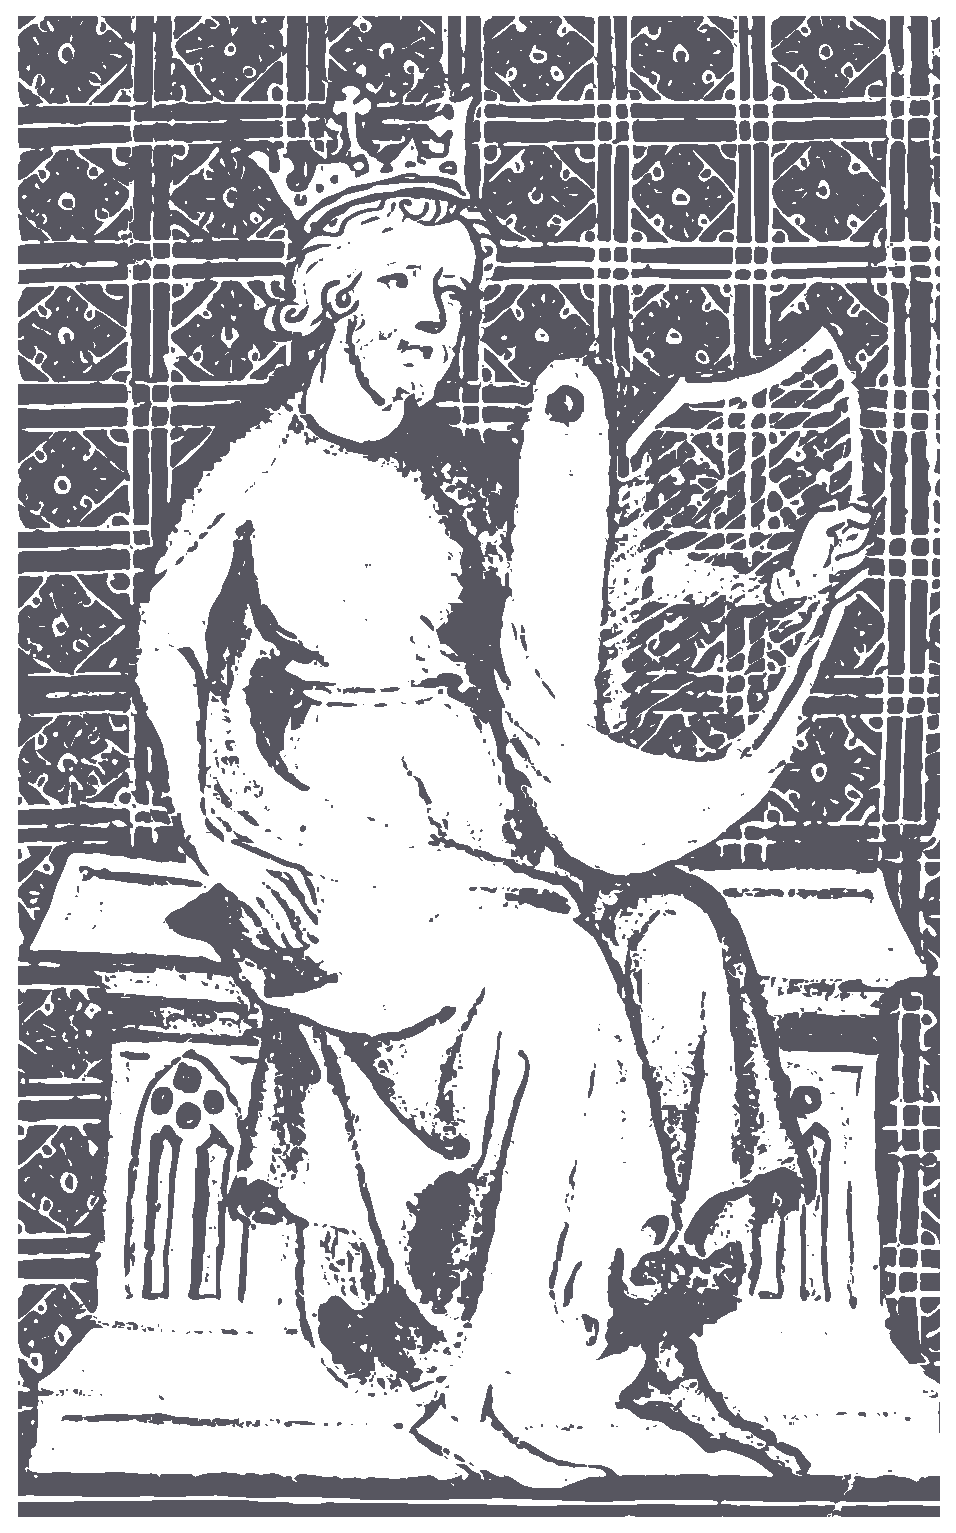
\includegraphics[scale=.6]{david.eps}
   \par
   \vspace{5ex}
   	\textsc{\Huge{The Daily Office}}
   \end{center}
\section{The Fore-Office}
\fancyhead[RE,LO]{The Fore-Office}
\rub{The Minister shall begin the Major Hours by reading of the following Scriptures.}
\begin{multicols}{2}
\seas{Morning}
The \textsc{Lord} is in his holy temple: let all the earth keep silence before him.\vr{Hab. 2:20}
\par
  \vr{Ps. 122:1}I was glad when they said unto me, We will go into the house of the \textsc{Lord}.
    \par
    Let the words of my mouth, and the meditation of my heart, be alway acceptable in thy sight, O \textsc{Lord}, my strength and my redeemer.\vr{Ps. 19:14}
    \par
    O send out thy light and thy truth, that they may lead me, and bring me unto thy holy hill, and to thy dwelling.\vr{Ps. 43:3}
    \par
    Thus saith the high and lofty One that inhabiteth eternity, whose name is Holy; I dwell in the high and holy place, with him also that is of a contrite and humble spirit, to revive the spirit of the humble, and to revive the heart of the contrite ones.\vr{Is. 57:15}
    \seas{Evening}
    Let my prayer be set forth in thy sight as the incense; and let the lifting up of my hands be an evening sacrifice.\vr{Ps. 141:2}
    \par
    The \textsc{Lord} is in his holy temple: let all the earth keep silence before him.\vr{Hab. 2:20}
    \par
    \textsc{Lord}, I have loved the habitation of thy house, and the place where thine honour dwelleth.\vr{Ps.26:8}
    \par
    O worship the \textsc{Lord} in the beauty of holiness; let the whole earth stand in awe of him.\vr{Ps. 96:9}
    \par
    Let the words of my mouth, and the meditation of my heart, be alway acceptable in thy sight, O \textsc{Lord}, my strength and my redeemer.\vr{Ps. 19:14-15}
%    \par
	\seas{Advent}
	Repent ye, for the Kingdom of heaven is at hand.\vr{Matt. 3:2}
	\par
	For, behold, the darkness shall cover the earth, and gross darkness the people: but the Lord shall arise upon thee, and his glory shall be seen upon thee. \vr{Is. 40:2}
	\par
    O Lord, Almighty God of our fathers, whom all men fear, and tremble before thy power; for the majesty of thy glory cannot be borne, and thine angry threatening toward sinners is importable: \vr{Mann. 1,5}
%    \par
	\seas{Christmas}
	Behold, I bring you good tidings of great joy, which shall be to all people. For unto you is born this day in the city of David a Saviour, which is Christ the Lord.\vr{Lk. 2:10-11}
	\par
	Herein was the love of God manifested in us, that God hath sent his only begotten Son into the world, that we might live through him. \vr{1 Jn. 4:9}
	\par
	Thy merciful promise is unmeasurable and unsearchable; for thou art the most high Lord, of great compassion, longsuffering, very merciful, and repentest of the evils of men. \vr{Mann. 6-7}
%	\par
	\seas{Epiphany}
	And the Gentiles shall come to thy light, and kings to the brightness of thy rising.\vr{Is. 60:3}\par
	From the rising of the sun even unto the going down of the same my Name shall be great among the Gentiles; and in every place incense shall be offered unto my Name, and a pure offering: for my Name shall be great among the heathen, saith the \textsc{Lord} of hosts.\vr{Mal. 1:11}
	\par
%    Awake, awake; put on thy strength, O Zion; put on thy beautiful garments, O Jerusalem.\vr{Is. 52:1}
%    \par
    Thou, O Lord, according to thy great goodness hast promised repentance and forgiveness to them that have sinned against thee: and of thine infinite mercies hast appointed repentance unto sinners, that they may be saved. \vr{Mann. 8}
%    \par
	\seas{Lent}
	Rend your heart, and not your garments, and turn unto the \textsc{Lord} your God: for he is gracious and merciful, slow to anger, and of great kindness, and repenteth him of the evil.\vr{Jl. 2:13}\par
    The sacrifices of God are a broken spirit: a broken and a contrite heart, O God, thou wilt not despise.\vr{Psalm 51:17}\par
    I have sinned, O Lord, I have sinned, and I acknowledge mine iniquities: wherefore, I humbly beseech thee, forgive me, O Lord, forgive me, and destroy me not with mine iniquities. \vr{Mann. 12}
%    \par
    \seas{Passiontide}
    Is it nothing to you, all ye that pass by? behold, and see if there be any sorrow like unto my sorrow which is done unto me, wherewith the LORD hath afflicted me.\vr{Lam. 1:12}\par
    Be not angry with me for ever, by reserving evil for me; neither condemn me to the lower parts of the earth. For thou art the God, even the God of them that repent; and in me thou wilt shew all thy goodness: for thou wilt save me, that am unworthy, according to thy great mercy. \vr{Mann. 13}
	\seas{Eastertide}
	He is risen. The Lord is risen indeed.\vr{Mk. 16:6}
	\par
    This is the day which the \textsc{Lord} hath made; we will rejoice and be glad in it.\vr{Psalm 118:24}
    \par
    I will praise thee for ever all the days of my life: for all the powers of the heavens do praise thee, and thine is the glory for ever and ever. Amen. \vr{Mann. 15}
%    \par
	\seas{Ascensiontide}
	Christ is not entered into the holy places made with hands, which are the figures of the true; but into heaven itself, now to appear in the presence of God for us.\vr{Heb. 9:24}
	\par
	Seeing that we have a great High Priest, that is passed into the heavens, Jesus the Son of God, let us come boldly unto the throne of grace, that we may obtain mercy, and find grace to help in time of need.\vr{Heb. 4:14,16}
%	\par
	\seas{Whitsuntide}
	Ye shall receive power, after that the Holy Ghost is come upon you: and ye shall be witnesses unto me both in Jerusalem, and in all Jud{\ae}a, and in Samaria, and unto the uttermost part of the earth.\vr{Acts 1:8}
	\par
    Because ye are sons, God hath sent forth the Spirit of his Son into your hearts, crying, Abba, Father.\vr{Gal. 4:6}
%    \par
	\seas{Trinitytide}
	Holy, holy, holy, Lord God Almighty, which was, and is, and is to come.\vr{Rev. 4:8}
	\par
	Holy, holy, holy, is the LORD of hosts: the whole earth is full of his glory. \vr{Is. 6:3}
	\par
	God is love; and he that abideth in love abideth in God and God in him.\vr{1 Jn. 4:16}
%	\par
%	\seas{The Blessed Sacrament}
%	Whoso eateth my flesh, and drinketh my blood, hath eternal life; and I will raise him up at the last day. \vr{Jn. 6:54}
%	\par
%	The cup of blessing which we bless, is it not the communion of the blood of Christ? The bread which we break, is it not the communion of the body of Christ? \vr{1 Cor. 10:16}
	\seas{Blessed Sacrament}
	I am the living bread which came down from heaven: if any man eat of this bread, he shall live for ever: and the bread that I will give is my flesh, which I will give for the life of the world. \vr{Jn. 6:51}\par
	But when they came to Jesus, and saw that he was dead already, they brake not his legs: but one of the soldiers with a spear pierced his side, and forthwith came there out blood and water.\vr{Jn.19:33-4}\par
%	Take my yoke upon you, and learn of me; for I am meek and lowly in heart: and ye shall find rest unto your souls. \vr{Matt. 11:29}
	For God so loved the world, that he gave his only begotten Son, that whosoever believeth in him should not perish, but have everlasting life. \vr{Jn. 3:16}
	\seas{Transfiguration}
	Arise, shine; for thy light is come, and the glory of the Lord is risen upon thee. \vr{Is. 60:1}
%	\seas{The Holy Name of Jesus}
%	And when eight days were accomplished for the circumcising of the child, his name was called \textsc{Jesus}, which was so named of the angel before he was conceived in the womb. \vr{Lk. 2:21}
%	\seas{Christ the King}
%	I will extol my God, and my soul shall praise the King of Heaven, and shall rejoice in his greatness. \vr{Tob. 13:7}
%	\par
%	For it pleased the Father that in him should all fulness dwell; and, having made peace through the blood of his cross, by him to reconcile all things unto himself; by him, I say, whether they be things in earth, or things in heaven. \vr{Col. 1:19}
%	\seas{The Holy Rood}
%	But God forbid that I should glory, save in the cross of our Lord Jesus Christ, by whom the world is crucified unto me, and I unto the world. \vr{Gal. 6:14}
	\seas{The Blessed Virgin Mary}
	Therefore the Lord himself shall give you a sign; Behold, a virgin shall conceive, and bear a son, and shall call his name Immanuel. \vr{Is. 6:14}
	\par
	Strength and honour are her clothing; and she shall rejoice in time to come. She openeth her mouth with wisdom; and in her tongue is the law of kindness. \vr{Prov. 31:25-6}
%	\seas{The Holy Angels}
%	Bless the Lord, ye his angels, that excel in strength, that do his commandments, hearkening unto the voice of his word. \vr{Ps. 103:20}
%	\par
%	Again, the kingdom of heaven is like unto a net, that was cast into the sea, and gathered of every kind: which, when it was full, they drew to shore, and sat down, and gathered the good into vessels, but cast the bad away. So shall it be at the end of the world: the angels shall come forth, and sever the wicked from among the just. \vr{Matt. 13:47-9}
%	\seas{The Holy Apostles}
%	The righteous shall shine, and run to and fro like sparks among the stubble. They shall judge the nations, and have dominion over the people, and their Lord shall reign for ever. \vr{Wis. 3:7}
%	\seas{The Holy Martyrs}
%	These be they that have put off mortal clothing, and put on the immortal, and have confessed the Name of God: now are they crowned, and receive palms. \vr{2 Esdras 2:45}
%	\par
%	My soul drew near even unto death. They compassed me on every side, and there was no man to help me: I looked for the succour of men, but there was none. Then I thought upon thy mercy, O Lord. My prayer was heard: for thou savedst me from destruction. \vr{Sir. 51:6,8,11-2}
%	\seas{Holy Bishops \& Priests}
%	He blessed him with glory, that he should execute the office of the priesthood, to bless the people in his Name, and to offer sacrifices to the Lord, incense, and a sweet savour. \vr{Sir. 44:15}
%	\seas{Holy Confessors \& Monks}
%	Blessed is the man that is found without blemish: and hath not gone after gold. Who is he? And we will call him blessed: for wonderful things hath he doen among his people. \vr{Sir. 31:8}
%	\seas{Holy Women}
%	Who can find a virtuous woman? For her price is far above rubies. The heart of her husband doth safely trust in her, so that he shall have no need of spoil. \vr{Prov. 31:10-1}
	\seas{Saints}
	But the souls of the righteous are in the hand of God, and there shall no torment touch them.\vr{Wis. 3:1}\par
	Look at the generations of old, and see; did ever any trust in the Lord, and was confounded? \vr{Sir. 2:10}
	\par
	The righteous shall shine, and run to and fro like sparks among the stubble. They shall judge the nations, and have dominion over the people, and their Lord shall reign for ever. \vr{Wis. 3:7}
	\seas{Dedication of a Church}
	And I heard a great voice out of heaven, saying, Behold the tabernacle of God is with men, and he will dwell with them, and they shall be his people, and God himself shall be with them, and be their God.\vr{Rev. 21:3}
	\par
	And the Lord appeared to Solomon by night, and said unto him, I have heard thy prayer, and have chosen this place to myself for an house of sacrifice. For now have I chosen and sanctified this house, that my name may be there for ever: and mine eyes and mine heart shall be there perpetually. \vr{2 Chron. 7:12,16}
	\par
	And the temple of God was opened in heaven, and there was seen in his temple the ark of his testament: and there were lightnings, and voices, and thunderings, and an earthquake, and great hail. And there appeared a great wonder in heaven; a woman clothed with the sun, and the moon under her feet, and upon her head a crown of twelve stars: and she being with child cried, travailing in birth, and pained to be delivered. \vr{Rev. 11:19-12:2}
\end{multicols}
\subsection{The General Confession}
\lett{D}{early} beloved brethren, the Scripture moveth us, in sundry places, to acknowledge and confess our manifold sins and wickedness; and that we should not dissemble nor cloak them before the face of Almighty God our heavenly Father; but confess them with an humble, lowly, penitent, and obedient heart; to the end that we may obtain forgiveness of the same, by his infinite goodness and mercy. And although we ought, at all times, humbly to acknowledge our sins before God; yet ought we chiefly so to do, when we assemble and meet together to render thanks for the great benefits that we have received at his hands, to set forth his most worthy praise, to hear his most holy Word, and to ask those things which are requisite and necessary, as well for the body as the soul. Wherefore I pray and beseech you, as many as are here present, to accompany me with a pure heart, and humble voice, unto the throne of the heavenly grace, saying--
\rub{or}
\lett{L}{et} us humbly confess our sins unto Almighty God.
\rub{To be prayed by all kneeling,}
\lett{A}{lmighty} and most merciful Father; We have erred, and strayed from thy ways like lost sheep. We have followed too much the devices and desires of our own hearts. We have offended against thy holy laws. We have left undone those things which we ought to have done; And we have done those things which we ought not to have done; And there is no health in us. But thou, O Lord, have mercy upon us, miserable offenders. Spare thou those, O God, who confess their faults. Restore thou those who are penitent; According to thy promises declared unto mankind in Christ Jesus our Lord. And grant, O most merciful Father, for his sake; That we may hereafter live a godly, righteous, and sober life, To the glory of thy holy Name. Amen.
\subsection{The Absolution}
\rub{The Priest stands and declares,}
\lett{A}{lmighty} God, the Father of our Lord Jesus Christ, who desireth not the death of a sinner, but rather that he may turn from his wickedness and live, hath given power, and commandment, to his Ministers, to declare and pronounce to his people, being penitent, the Absolution and Remission of their sins. He pardoneth and {\ding{64}} absolveth all those who truly repent, and unfeignedly believe his holy Gospel.
\par
Wherefore let us beseech him to grant us true repentance, and his Holy Spirit, that those things may please him which we do at this present; and that the rest of our life hereafter may be pure and holy; so that at the last we may come to his eternal joy; through Jesus Christ our Lord. Amen.
\rub{When the Minister is not a Priest, he stands and says instead,}
\lett{G}{rant}, we beseech thee, merciful Lord, to thy faithful people pardon and peace, that they may be cleansed from all their sins, and serve thee with a quiet mind; through Jesus Christ our Lord. Amen.
\rub{or}
\lett{G}{od} Almighty have mercy upon us, forgive us our sins, and bring us to everlasting life. Amen.
\lett{T}{he} Almighty and merciful Lord grant unto us pardon, absolution, and remission of our sins. Amen.
\rub{The Minister kneeling, all say,}
\lett{O}{ur} Father, who art in heaven, Hallowed be thy Name. Thy kingdom come. Thy will be done on earth, As it is in heaven. Give us this day our daily bread. And forgive us our trespasses, As we forgive those who trespass against us. And lead us not into temptation; But deliver us from evil: For thine is the kingdom, and the power, and the glory, for ever and ever. Amen.
\par\noindent
\lett{H}{ail} Mary, full of grace; The Lord is with thee; Blessed art thou amongst women, And blessed is the fruit of thy womb, Jesus. Holy Mary, Mother of God, Pray for us sinners, now and at the hour of our death. Amen.
\section{The Order of Mattins}
\fancyhead[RE,LO]{Morning Prayer}
\elcol{℣. O Lord, {\ding{61}} open thou our lips.}{℣. Dómine, {\ding{61}} lábia nostra apéries.}
\elcol{℟. And our mouth shall show forth thy praise.}{℟. Et os nostrum annuntiábit laudem tuam.}
\elcol{℣. O God, {\ding{64}} make speed to save us.}{℣. Deus, {\ding{64}} in adiutórium nostrum inténde.}
\elcol{℟. O Lord, make haste to help us.}{℟. Dómine, ad adiuvándum nos festína.}
\elcol{℣. Glory be to the Father, and to the Son, and to the Holy Ghost.}{℣. Glória Patri, et Fílio, * et Spirítui Sancto:}
\elcol{℟. As it was in the beginning, is now, and ever shall be, world without end. Amen.}{℟. Sicut erat in princípio, et nunc, et semper, * et in sǽcula s{\ae}culórum. Amen.}
\elcol{℣. Praise ye the Lord.}{℣. Laudáte Dominum.}
\elcol{℟. The Lord's Name be praised.}{℟. Sit Nomen Domini Benedictum.}
\subsection{The Invitatory}
\rub{Then shall be said or sung the following Canticle; except on those days for which other Canticles are appointed;\\
On the appointed days, the following antiphons may be sung or said at the indicated places throughout the \textit{Venite}.}
\par
\inv{On the Sundays in Advent:} Our King and Saviour draweth nigh; * O come, let us adore him.
\par
\inv{From Christmas Day until the Epiphany:} Alleluia. Unto us a child is born; * O come, let us adore him. Alleluia.
\par
\inv{On the Epiphany and seven days after, and on the Feast of the Transfiguration:} The Lord hath manifested forth his glory; * O come, let us adore him.
\par
\inv{From Low Sunday until Ascension Day:} Alleluia. The Lord is risen indeed; * O come let us adore him. Alleluia.
\par
\inv{From Ascension Day until Whitsunday:} Alleluia. Christ the Lord ascended into heaven; * O come, let us adore him. Alleluia.
\par
\inv{On Whitsunday and six days after:} Alleluia. The Spirit of the Lord filleth the world; * O come, let us adore him. Alleluia.
\par
\inv{On Sundays in Trinitytide and optionally on ferial days:} Father, Son, and Holy Ghost, One God; * O come, let us adore him.
\par
\inv{On the Purification and the Annunciation:} The Word was made flesh; * O come, let us adore him.
\par
\inv{On other Festivals for which a proper Epistle and Gospel are ordered:} The Lord is glorious in his saints; * O come, let us adore him.
\subsection{Venite, exultemus Domino.}
\elcol{\lett{O}{Come} let us sing unto the \textsc{Lord}; * let us heartily rejoice in the strength of our salvation.
\par
Let us come before his presence with thanksgiving; * and show ourselves glad in him with psalms.
\par
For the \textsc{Lord} is a great God; * and a great King above all gods.
\par
In his hand are all the corners of the earth; * and the strength of the hills is his also.
\par
The sea is his, and he made it; * and his hands prepared the dry land.
\par
O come, let us worship and fall down, * and kneel before the \textsc{Lord} our Maker.
\par
For he is the Lord our God; * and we are the people of his pasture, and the sheep of his hand.
}{\lett{V}{eníte}, exsultémus Dómino, jubilémus Deo, salutári nostro:\par
pr{\ae}occupémus fáciem ejus in confessióne, et in psalmis jubilémus ei.\par
Quóniam Deus magnus Dóminus, et Rex magnus super omnes deos, quóniam non repéllet Dóminus plebem suam:\par
quia in manu ejus sunt omnes fines terr{\ae}, et altitúdines móntium ipse cónspicit.\par
Quóniam ipsíus est mare, et ipse fecit illud, et áridam fundavérunt manus ejus\par
veníte, adorémus, et procidámus ante Deum: plorémus coram Dómino, qui fecit nos,\par
quia ipse est Dóminus, Deus noster; nos autem pópulus ejus, et oves páscu{\ae} ejus.
}
\rub{First Ending}
\elcol{O worship the \textsc{Lord} in the beauty of holiness; * let the whole earth stand in awe of him.\par
For he cometh, for he cometh to judge the earth; * and with righteousness to judge the world, and the peoples with his truth.\par
Glory be to the Father, and to the Son, and to the Holy Ghost.\par
As it was in the beginning, is now, and ever shall be, world without end. Amen.
}{Tóllite hóstias, et introíte in átria ejus: * adoráte Dóminum in átrio sancto ejus.\par
Judicábit orbem terr{\ae} in {\ae}quitáte, * et pópulos in veritáte sua.\par
Glória Patri, et Fílio, * et Spirítui Sancto:\par
Sicut erat in princípio, et nunc, et semper, * et in sǽcula s{\ae}culórum. Amen.
}\par
\rub{Second Ending}
\elcol{To-day if ye will hear his voice, harden not your hearts * as in the provocation, and as in the day of temptation in the wilderness;\par
When your fathers tempted me, * proved me, and saw my works.\par
Forty years long was I grieved with this generation, and said, * It is a people that do err in their hearts, for they have not known my ways:\par
Unto whom I sware in my wrath, * that they should not enter into my rest.
\par
Glory be to the Father, and to the Son, and to the Holy Ghost.\par
As it was in the beginning, is now, and ever shall be, world without end. Amen.
}{Hódie, si vocem ejus audiéritis, nolíte obduráre corda vestra, sicut in exacerbatióne secúndum diem tentatiónis in desérto: ubi tentavérunt me patres vestri, probavérunt et vidérunt ópera mea.
\par
Quadragínta annis próximus fui generatióni huic, et dixi; Semper hi errant corde, ipsi vero non cognovérunt vias meas: quibus jurávi in ira mea; Si introíbunt in réquiem meam.
\par
Glória Patri, et Fílio, * et Spirítui Sancto:\par
Sicut erat in princípio, et nunc, et semper, * et in sǽcula s{\ae}culórum. Amen.
}
\rub{After the Invitatory, a hymn may be sung.\\
Then shall be sung or said a portion of the Psalms according to the use of this Book. After each Psalm (or Psalm portion) and the \textit{Benedictus} shall be prayed the \textit{Gloria Patri.}\\
After which shall be read the First Lesson, according to the Daily Office Lectionary.}
\subsection{The First Canticle}
\subsubsection{Te Deum}
\rub{The Te Deum is prayed on all Sundays (outside Advent \& Lent) and Feast Days.}
\elcol{	
\lett{W}{e} praise thee, O God; we acknowledge thee to be the Lord.\par
All the earth doth worship thee, the Father everlasting.\par
    To thee all Angels cry aloud; the Heavens, and all the Powers therein;\par
    To thee Cherubim and Seraphim continually do cry,\par
    Holy, Holy, Holy, Lord God of Sabaoth;\par
    Heaven and earth are full of the Majesty of thy glory.\par
    The glorious company of the Apostles praise thee.\par
    The goodly fellowship of the Prophets praise thee.\par
    The noble army of Martyrs praise thee.\par
    The holy Church throughout all the world doth acknowledge thee;\par
    The Father of an infinite Majesty;\par
    Thine adorable, true and only Son;\par
    Also the Holy Ghost the Comforter.
\lett{T}{hou} art the King of Glory, O Christ.\par
Thou art the everlasting Son of the Father.\par
    When thou tookest upon thee to deliver man, thou didst humble thyself to be born of a Virgin.\par
    When thou hadst overcome the sharpness of death, thou didst open the Kingdom of Heaven to all believers.\par
    Thou sittest at the right hand of God, in the glory of the Father.\par
    We believe that thou shalt come to be our Judge.\par
    We therefore pray thee, help thy servants, whom thou hast redeemed with thy precious blood.\par
    Make them to be numbered with thy Saints, in glory everlasting.
\lett{O}{Lord}, save thy people, and bless thine heritage.\par
Govern them and lift them up for ever.\par
    Day by day we magnify thee;\par
    And we worship thy Name ever, world without end.\par
    Vouchsafe, O Lord, to keep us this day without sin.\par
    O Lord, have mercy upon us, have mercy upon us.\par
    O Lord, let thy mercy be upon us, as our trust is in thee.\par
    O Lord, in thee have I trusted; let me never be confounded.}
{
\lett{T}{e} Deum laudámus: * te Dóminum confitémur.\par
Te {\ae}térnum Patrem * omnis terra venerátur.\par
Tibi omnes Ángeli, * tibi C{\ae}li, et univérs{\ae} Potestáte\par
Tibi Chérubin et Séraphin * incessábili voce proclámant:\par
Sanctus, Sanctus, Sanctus * Dóminus Deus Sábaoth.\par
Pleni sunt c{\ae}li et terra * majestátis glóri{\ae} tu{\ae}.\par
Te gloriósus * Apostolórum chorus,\par
Te Prophetárum * laudábilis númerus,\par
Te Mártyrum candidátus * laudat exércitus.\par
Te per orbem terrárum * sancta confitétur Ecclésia,\par
Patrem * imméns{\ae} majestátis;\par
Venerándum tuum verum * et únicum Fílium;\par
Sanctum quoque * Paráclitum Spíritum.
\lett{T}{u} Rex glóri{\ae}, * Christe.\par
Tu Patris * sempitérnus es Fílius.\par
Tu, ad liberándum susceptúrus hóminem: * non horruísti Vírginis úterum.\par
Tu, devícto mortis acúleo, * aperuísti credéntibus regna c{\ae}lórum.\par
Tu ad déxteram Dei sedes, * in glória Patris.\par
Judex créderis * esse ventúrus. \par
Te ergo quǽsumus, tuis fámulis súbveni, * quos pr{\ae}cióso sánguine redemísti.\par
{\AE}térna fac cum Sanctis tuis * in glória munerári.
\lett{S}{alvum} fac pópulum tuum, Dómine, * et bénedic hereditáti tu{\ae}.\par
Et rege eos, * et extólle illos usque in {\ae}térnum.\par
Per síngulos dies * benedícimus te.\par
Et laudámus nomen tuum in sǽculum, * et in sǽculum sǽculi.\par
Dignáre, Dómine, die isto * sine peccáto nos custodíre.\par
Miserére nostri, Dómine, * miserére nostri.\par
Fiat misericórdia tua, Dómine, super nos, * quemádmodum sperávimus in te.\par
In te, Dómine, sperávi: * non confúndar in {\ae}térnum.
}
\subsubsection{Benedictus es, Domine}
\rub{The Benedictus es, Domine (or another daily canticle) is prayed on all ferial days.}
\elcol{\lett{B}{lessed} art thou, O Lord God of our fathers; * praised and exalted above all for ever.\par
    Blessed art thou for the Name of thy Majesty; * praised and exalted above all for ever.\par
    Blessed art thou in the temple of thy holiness; * Praised and exalted above all for ever.\par
    Blessed art thou that beholdest the depths, and dwellest between the Cherubim: * praised and exalted above all for ever.\par
    Blessed art thou on the glorious throne of thy Kingdom: * praised and exalted above all for ever.\par
    Blessed art thou in the firmament of heaven: * praised and exalted above all for ever.
}{\lett{B}{enedictus} es, Domine Deus patrum nostrorum: et laudabilis, et gloriosus, et superexaltatus in s{\ae}cula.\par
Et benedictum nomen glori{\ae} tu{\ae} sanctum: et laudabile, et superexaltatum in omnibus s{\ae}culis.\par
Benedictus es in templo sancto glori{\ae} tu{\ae}: et superlaudabilis, et supergloriosus in s{\ae}cula.\par
Benedictus es in throno regni tui: et superlaudabilis, et superexaltatus in s{\ae}cula.\par
Benedictus es, qui intueris abyssos, et sedes super cherubim: et laudabilis, et superexaltatus in s{\ae}cula.\par
Benedictus es in firmamento c{\ae}li: et laudabilis et gloriosus in s{\ae}cula.}
\rub{After the Second Lesson, a hymn may be said or sung followed by the \textit{Benedictus},}
\subsection{The Second Canticle}
\subsubsection{Benedictus}
\englat{	
\lett{B}{lessed} {\ding{64}} be the Lord God of Israel; * for he hath visited and redeemed his people;\\
    And hath raised up a mighty salvation for us, * in the house of his servant David;\\
    As he spake by the mouth of his holy Prophets, * which have been since the world began;\\
    That we should be saved from our enemies, * and from the hand of all that hate us.\par
    To perform the mercy promised to our forefathers, * and to remember his holy covenant;\\
    To perform the oath which he sware to our forefather Abraham, * that he would give us;\\
    That we being delivered out of the hand of our enemies * might serve him without fear;\\
    In holiness and righteousness before him, * all the days of our life.\\
    And thou, child, shalt be called the prophet of the Highest: * for thou shalt go. before the face of the Lord to prepare his ways;\\
    To give knowledge of salvation unto his people * for the remission of their sins,\\
    Through the tender mercy of our God; * whereby the day-spring from on high hath visited us;\\
    To give light to them that sit in darkness, and in the shadow of death, * and to guide our feet into the way of peace.}
{\lett{B}{enedictus} {\ding{64}} Dóminus, Deus Isra{\"e}l: * quia visitávit, et fecit redemptiónem plebi su{\ae}:\\
Et eréxit cornu salútis nobis: * in domo David, púeri sui.\\
Sicut locútus est per os sanctórum, * qui a sǽculo sunt, prophetárum ejus:\\
Salútem ex inimícis nostris, * et de manu ómnium, qui odérunt nos.\\
Ad faciéndam misericórdiam cum pátribus nostris: * et memorári testaménti sui sancti.\\
Jusjurándum, quod jurávit ad Ábraham patrem nostrum, * datúrum se nobis:\\
Ut sine timóre, de manu inimicórum nostrórum liberáti, * serviámus illi.\\
In sanctitáte, et justítia coram ipso, * ómnibus diébus nostris.\\
Et tu, puer, Prophéta Altíssimi vocáberis: * pr{\ae}íbis enim ante fáciem Dómini, paráre vias ejus:\\
Ad dandam sciéntiam salútis plebi ejus: * in remissiónem peccatórum eórum:\\
Per víscera misericórdi{\ae} Dei nostri: * in quibus visitávit nos, óriens ex alto:\\
Illumináre his, qui in ténebris, et in umbra mortis sedent: * ad dirigéndos pedes nostros in viam pacis.
}
\subsection{The Apostles' Creed}
\elcol{
\lett{I}{Believe} in God the Father Almighty, Maker of heaven and earth: And in Jesus Christ his only Son our Lord: Who was conceived by the Holy Ghost, Born of the Virgin Mary: Suffered under Pontius Pilate, Was crucified, dead, and buried: He descended into hell; The third day he rose again from the dead: He ascended into heaven, And sitteth on the right hand of God the Father Almighty: From thence he shall come to judge the quick and the dead.\par
    I believe in the Holy Ghost: The holy Catholic Church; The Communion of Saints: The Forgiveness of sins: The Resurrection of the body: {\ding{64}} And the Life everlasting. Amen.
}{
\lett{C}{redo} in Deum, Patrem omnipoténtem, Creatórem c{\ae}li et terr{\ae}. Et in Jesum Christum, Fílium ejus únicum, Dóminum nostrum: qui concéptus est de Spíritu Sancto, natus ex María Vírgine, passus sub Póntio Piláto, crucifíxus, mórtuus, et sepúltus: descéndit ad ínferos; tértia die resurréxit a mórtuis; ascéndit ad c{\ae}los; sedet ad déxteram Dei Patris omnipoténtis: inde ventúrus est judicáre vivos et mórtuos.\par
     Credo in Spíritum Sanctum, sanctam Ecclésiam cathólicam, Sanctórum communiónem, remissiónem peccatórum, carnis {\ding{64}} resurrectiónem, vitam {\ae}térnam. Amen.
 }
\rub{And after that, these Prayers following, the people devoutly kneeling; the Minister first pronouncing (the words in parentheses if he is not in major orders),}
\elcol{℣. The Lord be with you. (O Lord, hear my prayer.)}{℣. Dóminus vobíscum. (Dómine, exáudi oratiónem meam.)}
\elcol{℟. And with thy spirit. (And let my cry come unto thee.)}{℟. Et cum spiritu tuo. (Et clamor meus ad te véniat.)}
\elcol{℣. Let us pray.}{℣. Orémus.}
\elcol{℣. Lord, have mercy upon us.}{℣. Kýrie, eléison.}
\elcol{℟. Christ, have mercy upon us.}{℟. Christe, eléison.}
\elcol{℣. Lord, have mercy upon us.}{℣. Kýrie, eléison.}
\subsection{Our Father}
\rub{All kneeling shall say the Lord's Prayer.}
\englat{
\lett{O}{ur} Father, who art in heaven, Hallowed be thy Name. Thy kingdom come. Thy will be done on earth, As it is in heaven. Give us this day our daily bread. And forgive us our trespasses, As we forgive those who trespass against us. And lead us not into temptation; But deliver us from evil. Amen.}
{
\lett{P}{ater} noster, qui es in c{\ae}lis, sanctificétur nomen tuum: advéniat regnum tuum: fiat volúntas tua, sicut in c{\ae}lo et in terra. Panem nostrum quotidiánum da nobis hódie: et dimítte nobis débita nostra, sicut et nos dimíttimus debitóribus nostris: et ne nos indúcas in tentatiónem: sed líbera nos a malo. Amen.}
\subsection{The Preces}
\rub{The Minister, standing, shall say:}
\elcol{℣. O Lord, show thy mercy upon us.}{℣. Ostende nobis Domine misericordiam tuam.}
\elcol{℟. And grant us thy salvation.}{℟. Et salutare tuum da nobis.}
\elcol{℣. O God, make clean our hearts within us.}{℣. Cor mundum crea in nobis, O Deus.}
\elcol{℟. And take not thy Holy Spirit from us.}{℟. Et Spiritum Sanctum tuum ne auferas a nobis.}
\subsection{The Collects}
\rub{Then shall follow the Collect for the Day and then the following collects.}
\subsubsection{A Collect for Peace}
\lett{O}{God}, who art the author of peace and lover of concord, in knowledge of whom standeth our eternal life, whose service is perfect freedom; Defend us thy humble servants in all assaults of our enemies; that we, surely trusting in thy defence, may not fear the power of any adversaries, through the might of Jesus Christ our Lord. Amen.
\subsubsection{A Collect for Grace}
\lett{O}{Lord}, our heavenly Father, Almighty and everlasting God, who hast safely brought us to the beginning of this day; Defend us in the same with thy mighty power; and grant that this day we fall into no sin, neither run into any kind of danger; but that all our doings, being ordered by thy governance, may be righteous in thy sight; through Jesus Christ our Lord. Amen.
\subsection{Conclusion}
\elcol{℣. The Lord be with you. (O Lord, hear my prayer.)}{℣. Dóminus vobíscum. (Dómine, exáudi oratiónem meam.)}
\elcol{℟. And with thy spirit. (And let my cry come unto thee.)}{℟. Et cum spiritu tuo. (Et clamor meus ad te véniat.)}
\elcol{℣. Let us bless the Lord. (alleluia, alleluia.)}{℣. Benedicámus Dómino (allelúia, allelúia).}
\elcol{℟. Thanks be to God. (alleluia, alleluia.)}{℟. Deo grátias (allelúia, allelúia).}
\elcol{℣. May the souls {\ding{64}} of the faithful departed, through the mercy of God, rest in peace.}{℣. Fidélium ánim{\ae} {\ding{64}} per misericórdiam Dei requiéscant in pace.}
\elcol{℟. Amen.}{℟. Amen.}
\rub{The appropriate Marian Anthem (p. \pageref{mary}) may be said or sung here.}
\subsection{Third Collects}
\subsubsection{A Prayer for The President of the United States, and all in Civil Authority}
\lett{O}{Lord}, our heavenly Father, the high and mighty Ruler of the universe, who dost from thy throne behold all the dwellers upon earth; Most heartily we beseech thee, with thy favour to behold and bless thy servant THE PRESIDENT OF THE UNITED STATES, and all others in authority; and so replenish them with the grace of thy Holy Spirit, that they may always incline to thy will, and walk in thy way. Endue them plenteously with heavenly gifts; grant them in health and prosperity long to live; and finally, after this life, to attain everlasting joy and felicity; through Jesus Christ our Lord. Amen.
\subsubsection{A Prayer for the Clergy and People}
\lett{A}{lmighty} and everlasting God, from whom cometh every good and perfect gift; Send down upon our Bishops, and other Clergy, and upon the Congregations committed to their charge, the healthful Spirit of thy grace; and, that they may truly please thee, pour upon them the continual dew of thy blessing. Grant this, O Lord, for the honour of our Advocate arid Mediator, Jesus Christ. Amen.
\subsubsection{A Prayer for all Sorts \& Conditions of Men}
\lett{O}{God}, the Creator and Preserver of all mankind, we humbly beseech thee for all sorts and conditions of men; that thou wouldest be pleased to make thy ways known unto them, thy saving health unto all nations. More especially we pray for thy holy Church universal; that it may be so guided and governed by thy good Spirit, that all who profess and call themselves Christians may be led into the way of truth, and hold the faith in unity of spirit, in the bond of peace, and in righteousness of life. Finally, we commend to thy fatherly goodness all those who are any ways afflicted, or distressed, in mind, body, or estate; (especially those for whom our prayers are desired;) that it may please thee to comfort and relieve them, according to. their several necessities; giving them patience under their sufferings, and a happy issue out of all their afflictions. And this we beg for Jesus Christ's sake. Amen.
\subsubsection{A General Thanksgiving}
\rub{The General Thanksgiving may be said by the Congregation with the Minister.}
\lett{A}{lmighty} God, Father of all mercies, we, thine unworthy servants, do give thee most humble and hearty thanks for all thy goodness and loving-kindness to us and to all men; (to those who desire now to offer up their praises and thanksgivings for thy late mercies vouchsafed unto them.) We bless thee for our creation, preservation, and all the blessings of this life; but above all, for thine inestimable love in the redemption of the world by our Lord Jesus Christ; for the means of grace, and for the hope of glory. And, we beseech thee, give us that due sense of all thy mercies, that our hearts may he unfeignedly thankful; and that we show forth thy praise, not only with our lips, but in our lives, by giving up our selves to thy service, and by walking before thee in holiness and righteousness all our days; through Jesus Christ our Lord, to whom, with thee and the Holy Ghost, be all honour and glory, world without end. Amen.
\subsubsection{A Prayer of St. Chrysostom}
\lett{A}{lmighty} God, who hast given us grace at this time with one accord to make our common supplications unto thee; and dost promise that when two or three are gathered together in thy Name thou wilt grant their requests; Fulfil now, O Lord, the desires and petitions of thy servants, as may be most expedient for them; granting us in this world knowledge of thy truth, and in the world to come life everlasting. Amen.
\subsubsection{The Grace}
\lett{T}{he} grace of our Lord Jesus Christ, {\ding{64}} and the love of God, and the fellowship of the Holy Ghost, be with us all evermore. Amen.\par
\begin{center}
	\textsc{Here endeth the Order of Morning Prayer.}
\end{center}
\section{The Athanasian Creed}
\fancyhead[RE,LO]{The Athanasian Creed}
\rub{The Athanasian Creed shall be sung or said, standing, replacing the Apostles' Creed for the Major Hours on Christmas Day, Epiphany Day, Saint Matthias, Easter Day, Ascension Day, Whitsunday, Trinity Sunday, and on the Feasts of St. John Baptist, St. James, St. Matthew, Sts. Simon \& Jude, and St.Andrew.}
\elcol{
\lett{W}{hosoever} will be saved: before all things it is necessary that he hold the Catholick Faith.\par
Which Faith except every one do keep whole and undefiled: without doubt he shall perish everlastingly.
\par
And the Catholick Faith is this: That we worship one God in Trinity, and Trinity in Unity;\par
Neither confounding the Persons: nor dividing the Substance.\par
For there is one Person of the Father, another of the Son: and another of the Holy Ghost.\par
But the Godhead of the Father, of the Son, and of the Holy Ghost, is all one: the Glory equal, the Majesty co-eternal.\par
Such as the Father is, such is the Son: and such is the Holy Ghost.\par
The Father uncreate, the Son uncreate: and the Holy Ghost uncreate.\par
The Father incomprehensible, the Son incomprehensible: and the Holy Ghost incomprehensible.\par
The Father eternal, the Son eternal: and the Holy Ghost eternal.\par
And yet they are not three eternals: but one eternal.\par
As also there are not three incomprehensibles, nor three uncreated: but one uncreated, and one incomprehensible.\par
So likewise the Father is Almighty, the Son Almighty: and the Holy Ghost Almighty.\par
And yet they are not three Almighties: but one Almighty.\par
So the Father is God, the Son is God: and the Holy Ghost is God.\par
And yet they are not three Gods: but one God.\par
So likewise the Father is Lord, the Son Lord: and the Holy Ghost Lord.\par
And yet not three Lords: but one Lord.\par
For like as we are compelled by the Christian verity: to acknowledge every Person by himself to be God and Lord;\par
So are we forbidden by the Catholick Religion: to say there be three Gods, or three Lords.\par
The Father is made of none: neither created, nor begotten.\par
The Son is of the Father alone: not made, nor created, but begotten.\par
The Holy Ghost is of the Father (alone): neither made, nor created, nor begotten, but proceeding.\par
So there is one Father, not three Fathers; one Son, not three Sons: one Holy Ghost, not three Holy Ghosts.\par
And in this Trinity none is afore, or after other: none is greater, or less than another;\par
But the whole three Persons are co-eternal together: and co-equal.\par
So that in all things, as is aforesaid: the Unity in Trinity, and the Trinity in Unity is to be worshipped.\par
He therefore that will be saved: must thus think of the Trinity.
\par
Furthermore it is necessary to everlasting salvation: that he also believe rightly the Incarnation of our Lord Jesus Christ.\par
For the right Faith is that we believe and confess: that our Lord Jesus Christ, the Son of God, is God and Man;\par
God, of the Substance of the Father, begotten before the worlds: and Man, of the Substance of his Mother, born in the world;\par
Perfect God, and Perfect Man: of a reasonable soul and human flesh subsisting;\par
Equal to the Father, as touching his Godhead: and inferior to the Father, as touching his Manhood.\par
Who although he be God and Man: yet he is not two, but one Christ;\
One, not by conversion of the Godhead into flesh: but by taking of the Manhood into God;\par
One altogether, not by confusion of Substance: but by unity of Person.\par
For as the reasonable soul and flesh is one man: so God and Man is one Christ.\par
Who suffered for our salvation: descended into hell, rose again the third day from the dead.\par
He ascended into heaven, he sitteth on the right hand of the Father, God Almighty: from whence he shall come to judge the quick and the dead.\par
At whose coming all men shall rise again with their bodies: and shall give account for their own works.\par
And they that have done good shall go into life everlasting: and they that have done evil into everlasting fire.
\par
This is the Catholick Faith: which except a man believe faithfully, he cannot be saved.\par
\par
Glory be to the Father, and to the Son: and to the Holy Ghost;
As it was in the beginning, is now, and ever shall be: world without end. Amen.
}
{\lett{Q}{uicúmque} vult salvus esse, * ante ómnia opus est, ut téneat cathólicam fidem:\par
Quam nisi quisque íntegram inviolatámque serváverit, * absque dúbio in {\ae}térnum períbit.
\par
Fides autem cathólica h{\ae}c est: * ut unum Deum in Trinitáte, et Trinitátem in unitáte venerémur.\par
Neque confundéntes persónas, * neque substántiam separántes.\par
Alia est enim persóna Patris, ália Fílii, * ália Spíritus Sancti:\par
Sed Patris, et Fílii, et Spíritus Sancti una est divínitas, * {\ae}quális glória, co{\ae}térna majéstas.\par
Qualis Pater, talis Fílius, * talis Spíritus Sanctus.\par
Increátus Pater, increátus Fílius, * increátus Spíritus Sanctus.\par
Imménsus Pater, imménsus Fílius, * imménsus Spíritus Sanctus.\par
{\ae}térnus Pater, {\ae}térnus Fílius, * {\ae}térnus Spíritus Sanctus.\par
Et tamen non tres {\ae}térni, * sed unus {\ae}térnus.\par
Sicut non tres increáti, nec tres imménsi, * sed unus increátus, et unus imménsus.\par
Simíliter omnípotens Pater, omnípotens Fílius, * omnípotens Spíritus Sanctus.\par
Et tamen non tres omnipoténtes, * sed unus omnípotens.\par
Ita Deus Pater, Deus Fílius, * Deus Spíritus Sanctus.\par
Ut tamen non tres Dii, * sed unus est Deus.\par
Ita Dóminus Pater, Dóminus Fílius, * Dóminus Spíritus Sanctus.\par
Et tamen non tres Dómini, * sed unus est Dóminus.\par
Quia, sicut singillátim unamquámque persónam Deum ac Dóminum confitéri christiána veritáte compéllimur: * ita tres Deos aut Dóminos dícere cathólica religióne prohibémur.\par
Pater a nullo est factus: * nec creátus, nec génitus.\par
Fílius a Patre solo est: * non factus, nec creátus, sed génitus.\par
Spíritus Sanctus a Patre (solo): * non factus, nec creátus, nec génitus, sed procédens.\par
Unus ergo Pater, non tres Patres: unus Fílius, non tres Fílii: * unus Spíritus Sanctus, non tres Spíritus Sancti.\par
Et in hac Trinitáte nihil prius aut postérius, nihil majus aut minus: * sed tot{\ae} tres persón{\ae} co{\ae}térn{\ae} sibi sunt et co{\ae}quáles.\par
Ita ut per ómnia, sicut jam supra dictum est, * et únitas in Trinitáte, et Trínitas in unitáte veneránda sit.\par
Qui vult ergo salvus esse, * ita de Trinitáte séntiat.
\par
Sed necessárium est ad {\ae}térnam salútem, * ut Incarnatiónem quoque Dómini nostri Jesu Christi fidéliter credat.\par
Est ergo fides recta ut credámus et confiteámur, * quia Dóminus noster Jesus Christus, Dei Fílius, Deus et homo est.\par
Deus est ex substántia Patris ante sǽcula génitus: * et homo est ex substántia matris in sǽculo natus.\par
Perféctus Deus, perféctus homo: * ex ánima rationáli et humána carne subsístens.\par
{\ae}quális Patri secúndum divinitátem: * minor Patre secúndum humanitátem.\par
Qui licet Deus sit et homo, * non duo tamen, sed unus est Christus.\par
Unus autem non conversióne divinitátis in carnem, * sed assumptióne humanitátis in Deum.\par
Unus omníno, non confusióne substánti{\ae}, * sed unitáte persón{\ae}.\par
Nam sicut ánima rationális et caro unus est homo: * ita Deus et homo unus est Christus.\par
Qui passus est pro salúte nostra: descéndit ad ínferos: * tértia die resurréxit a mórtuis.\par
Ascéndit ad c{\ae}los, sedet ad déxteram Dei Patris omnipoténtis: * inde ventúrus est judicáre vivos et mórtuos.\par
Ad cujus advéntum omnes hómines resúrgere habent cum corpóribus suis; * et redditúri sunt de factis própriis ratiónem.\par
Et qui bona egérunt, ibunt in vitam {\ae}térnam: * qui vero mala, in ignem {\ae}térnum.
\par
H{\ae}c est fides cathólica, * quam nisi quisque fidéliter firmitérque credíderit, salvus esse non póterit.\par
\par
Glória Patri, et Fílio, * et Spirítui Sancto: Sicut erat in princípio, et nunc, et semper, * et in sǽcula s{\ae}culórum. Amen.
}
%\section{The Hour of Prime}
\fancyhead[RE,LO]{The Hour of Prime}
\subsection{Introduction}
\englat
{
\textit{\scshape ℣.} O God, {\ding{64}} make speed to save us.\\
\textit{\scshape ℟.} O Lord, make haste to help us.\\
\textit{\scshape ℣.} Glory be to the Father, and to the Son, and to the Holy Ghost.\\
\textit{\scshape ℟.} As it was in the beginning, is now, and ever shall be, world without end. Amen.\\
\textit{\scshape ℣.} Praise ye the Lord.\\
\textit{\scshape ℟.} The Lord's Name be praised.\\
}
{
\textit{\scshape ℣.} Deus, {\ding{64}} in adjutorium nostrum intende.\\
\textit{\scshape ℟.} Domine, ad adjuvandum nos festina.\\
\textit{\scshape ℣.} Glória Patri, et Fílio, * et Spirítui Sancto:\\
\textit{\scshape ℟.} Sicut erat in princípio, et nunc, et semper, * et in sǽcula s{\ae}culórum. Amen.\\
\textit{\scshape ℣.} Laudate Dominum.\\
\textit{\scshape ℟.} Sit Nomen Domini Benedictum.\\
}
\subsection{Jam Lucis Ordo Sidere}
\englat{
Now that the daylight fills the sky,\\
We lift our hearts to God on high,\\
That he, in all we do or say,\\
Would keep us free from harm today.\\
\par
Would guard our hearts and tongues from strife;\\
From anger's din would hide our life;\\
From all ill sights would turn our eyes;\\
Would close our ears from vanities;\\
\par
Would keep our inmost conscience pure;\\
Our souls from folly would secure;\\
Would bid us check the pride of sense\\
With due and holy abstinence.\\
\par
So we, when this new day is gone,\\
And night in turn is drawing on,\\
With conscience by the world unstained,\\
Shall praise his Name for victory gained.\\
\par
All laud to God the Father be;\\
All praise, eternal Son, to thee;\\
All glory, as is ever meet,\\
To God the Holy Paraclete. Amen.
}{
Jam lucis orto sídere,\\
Deum precémur súpplices,\\
Ut in diúrnis áctibus\\
Nos servet a nocéntibus.\\
\par
Linguam refrénans témperet,\\
Ne litis horror ínsonet:\\
Visum fovéndo cóntegat,\\
Ne vanitátes háuriat.\\
\par
Sint pura cordis íntima,\\
Absístat et vecórdia;\\
Carnis terat supérbiam\\
Potus cibíque párcitas.\\
\par
Ut, cum dies abscésserit,\\
Noctémque sors redúxerit,\\
Mundi per abstinéntiam\\
Ipsi canámus glóriam.\\
\par
Deo Patri sit glória,\\
Ejúsque soli Fílio,\\
Cum Spíritu Paráclito,\\
Nunc et per omne sǽculum.\\
Amen.
}
\subsection{The Psalms}
\inv{Ant. throughout the Year:} Alleluia. *\\
\inv{Ant. in Advent:} Lo, now cometh. *\\
\inv{Ant. from Christmas until Candlemas.} Whom beheld ye. *\\
\inv{Ant. in Pre-Lent and Lent.} They that fear the Lord. *\\
\inv{Ant. in Eastertide.} Alleluia. *
\subsubsection{Psalm 54. \textit{Deus, in Nomine.}}
\rub{Sunday}
\lett{S}{ave} me, O God, for thy Name's sake, * and avenge me in thy strength.\par
2 Hear my prayer, O God, * and hearken unto the words of my mouth.\par
3 For strangers are risen up against me; * and tyrants, which have not God before their eyes, seek after my soul.\par
4 Behold, God is my helper; * the Lord is with them that uphold my soul.\par
5 He shall reward evil unto mine enemies: * destroy thou them in thy truth.\par
6 An offering of a free heart will I give thee, and praise thy Name, O \textsc{Lord}; * because it is so comfortable.\par
7 For he hath delivered me out of all my trouble; * and mine eye hath seen his desire upon mine enemies.
\subsubsection{Psalm 118. \textit{Confitemini Domino.}}
\rub{Sunday}
\lett{O}{Give} thanks unto the \textsc{Lord}, for he is gracious; * because his mercy endureth for ever.
\par
    2 Let Israel now confess that he is gracious, * and that his mercy endureth for ever.
\par
    3 Let the house of Aaron now confess, * that his mercy endureth for ever.
\par
    4 Yea, let them now that fear the \textsc{Lord} confess, * that his mercy endureth for ever.
\par
    5 I called upon the \textsc{Lord} in trouble; * and the \textsc{Lord} heard me at large.
\par
    6 The \textsc{Lord} is on my side; * I will not fear what man doeth unto me.
\par
    7 The \textsc{Lord} taketh my part with them that help me; * therefore shall I see my desire upon mine enemies.
\par
    8 It is better to trust in the \textsc{Lord}, * than to put any confidence in man.
\par
    9 It is better to trust in the \textsc{Lord}, * than to put any confidence in princes.
\par
    10 All nations compassed me round about; * but in the Name of the \textsc{Lord} will I destroy them.
\par
    11 They kept me in on every side, they kept me in, I say, on every side; * but in the Name of the \textsc{Lord} will I destroy them.
\par
    12 They came about me like bees, and are extinct even as the fire among the thorns; * for in the Name of the \textsc{Lord} I will destroy them.
\par
    13 Thou hast thrust sore at me, that I might fall; * but the \textsc{Lord} was my help.
\par
    14 The \textsc{Lord} is my strength, and my song; * and is become my salvation.
\par
    15 The voice of joy and health is in the dwellings of the righteous; * the right hand of the \textsc{Lord} bringeth mighty things to pass.
\par
    16 The right hand of the \textsc{Lord} hath the preeminence; * the right hand of the \textsc{Lord} bringeth mighty things to pass.
\par
    17 I shall not die, but live, * and declare the works of the \textsc{Lord}.
\par
    18 The \textsc{Lord} hath chastened and corrected me; * but he hath not given me over unto death.
\par
    19 Open me the gates of righteousness, * that I may go into them, and give thanks unto the \textsc{Lord}.
\par
    20 This is the gate of the \textsc{Lord}, * the righteous shall enter into it.
\par
    21 I will thank thee; for thou hast heard me, * and art become my salvation.
\par
    22 The same stone which the builders refused, * is become the head-stone in the corner.
\par
    23 This is the \textsc{Lord's} doing, * and it is marvellous in our eyes.
\par
    24 This is the day which the \textsc{Lord} hath made; * we will rejoice and be glad in it.
\par
    25 Help me now, O \textsc{Lord}: * O \textsc{Lord}, send us now prosperity.
\par
    26 Blessed be he that cometh in the Name of the \textsc{Lord}: * we have wished you good luck, we that are of the house of the \textsc{Lord}.
\par
    27 God is the \textsc{Lord}, who hath showed us light: * bind the sacrifice with cords, yea, even unto the horns of the altar.
\par
    28 Thou art my God, and I will thank thee; * thou art my God, and I will praise thee.
\par
    29 O give thanks unto the \textsc{Lord}; for he is gracious, * and his mercy endureth for ever.
\subsubsection{Psalm 119:I-II \textit{Beati immaculati.}}
\rub{Sunday, Monday, Wednesday, Friday}
\lett{B}{lessed} are those that are undefiled in the way, and walk in the law of the \textsc{Lord}.\par
2 Blessed are they that keep his testimonies, * and seek him with their whole heart;\par
3 Even they who do no wickedness, * and walk in his ways.\par
4 Thou hast charged * that we shall diligently keep thy commandments.\par
5 O that my ways were made so direct, * that I might keep thy statutes!\par
6 So shall I not be confounded, * while I have respect unto all thy commandments.\par
7 I will thank thee with an unfeigned heart, * when I shall have learned the judgments of thy righteousness.\par   
8 I will keep thy statutes1; * O forsake me not utterly.
\par
9 Wherewithal shall a young man cleanse his way? * even by ruling himself after thy word.\par
10 With my whole heart have I sought thee; * O let me not go wrong out of thy commandments.\par
11 Thy word have I hid within my heart, * that I should not sin against thee.\par
12 Blessed art thou, O \textsc{Lord}; * O teach me thy statutes.\par
13 With my lips have I been telling * of all the judgments of thy mouth.\par
14 I have had as great delight in the way of thy testimonies, * as in all manner of riches.\par
15 I will talk of thy commandments, * and have respect unto thy ways.\par
16 My delight shall be in thy statutes, * and I will not forget thy word.
\subsubsection{Psalm 119:III-IV \textit{Retribue servo tuo.}}
\rub{Sunday, Monday, Wednesday, Friday}
\lett{O}{Do} well unto thy servant; * that I may live, and keep thy word.\par
18 Open thou mine eyes; * that I may see the wondrous things of thy law.\par
19 I am a stranger upon earth; * O hide not thy commandments from me.\par
20 My soul breaketh out for the very fervent desire * that it hath alway unto thy judgments.\par
21 Thou hast rebuked the proud; * and cursed are they that do err from thy commandments.\par
22 O turn from me shame and rebuke; * for I have kept thy testimonies.\par
23 Princes also did sit and speak against me; * but thy servant is occupied in thy statutes.\par
24 For thy testimonies are my delight, * and my counsellors.
\par
25 My soul cleaveth to the dust; * O quicken thou me, according to thy word.
\par
    26 I have acknowledged my ways, and thou heardest me: * O teach me thy statutes.
\par
    27 Make me to understand the way of thy commandments; * and so shall I talk of thy wondrous works.
\par
    28 My soul melteth away for very heaviness; * comfort thou me according unto thy word.
\par
    29 Take from me the way of lying, * and cause thou me to make much of thy law.
\par
    30 I have chosen the way of truth, * and thy judgments have I laid before me.
\par
    31 I have stuck unto thy testimonies; * O \textsc{Lord}, confound me not.
\par
    32 I will run the way of thy commandments, * when thou hast set my heart at liberty.
\subsubsection{Psalm XIV-XV. \textit{Lucerna pedibus meis.}}
\rub{Tuesday, Thursday, Saturday}
\lett{T}{hy} word is a lantern unto my feet, * and a light unto my paths.
\par
    106 I have sworn, and am stedfastly purposed, * to keep thy righteous judgments.
\par
    107 I am troubled above measure: * quicken me, O \textsc{Lord}, according to thy word.
\par
    108 Let the free-will offerings of my mouth please thee, O \textsc{Lord}; * and teach me thy judgments.
\par
    109 My soul is alway in my hand; * yet do I not forget thy law.
\par
    110 The ungodly have laid a snare for me; * but yet I swerved not from thy commandments.
\par
    111 Thy testimonies have I claimed as mine heritage for ever; * and why? they are the very joy of my heart.
\par
    112 I have applied my heart to fulfil thy statutes alway, * even unto the end.
\par
I hate them that imagine evil things; * but thy law do I love.
\par
    114 Thou art my defence and shield; * and my trust is in thy word.
\par
    115 Away from me, ye wicked; * I will keep the commandments of my God.
\par
    116 O stablish me according to thy word, that I may live; * and let me not be disappointed of my hope.
\par
    117 Hold thou me up, and I shall be safe; * yea, my delight shall be ever in thy statutes.
\par
    118 Thou hast trodden down all them that depart from thy statutes; * for they imagine but deceit.
\par
    119 Thou puttest away all the ungodly of the earth like dross; * therefore I love thy testimonies.
\par
    120 My flesh trembleth for fear of thee; * and I am afraid of thy judgments.
\subsubsection{Psalm 119:XVI-XVII. \textit{Feci judicium.}}
\rub{Tuesday, Thursday, Saturday}
\lett{I}{Deal} with the thing that is lawful and right; * O give me not over unto mine oppressors.
\par
    122 Make thou thy servant to delight in that which is good, * that the proud do me no wrong.
\par
    123 Mine eyes are wasted away with looking for thy health, * and for the word of thy righteousness.
\par
    124 O deal with thy servant according unto thy loving mercy, * and teach me thy statutes.
\par
    125 I am thy servant; O grant me understanding, * that I may know thy testimonies.
\par
    126 It is time for thee, \textsc{Lord}, to lay to thine hand; * for they have destroyed thy law.
\par
    127 For I love thy commandments * above gold and precious stones.
\par
    128 Therefore hold I straight all thy commandments; * and all false ways I utterly abhor.
\par
    129 Thy testimonies are wonderful; * therefore doth my soul keep them.
\par
    130 When thy word goeth forth, * it giveth light and understanding unto the simple.
\par
    131 I opened my mouth, and drew in my breath; * for my delight was in thy commandments.
\par
    132 O look thou upon me, and be merciful unto me, * as thou usest to do unto those that love thy Name.
\par
    133 Order my steps in thy word; * and so shall no wickedness have dominion over me.
\par
    134 O deliver me from the wrongful dealings of men; * and so shall I keep thy commandments.
\par
    135 Show the light of thy countenance upon thy servant, * and teach me thy statutes.
\par
    136 Mine eyes gush out with water, * because men keep not thy law.
\rub{On Sundays in Trinitytide and after Epiphany until Septuagesimma, the Athanasian Creed may be added here.}
\inv{Ant. throughout the Year:} Alleluia. * O Give thanks unto the Lord, because his mercy endureth for ever. Alleluia.\\
\inv{Ant. in Advent:} Lo, now cometh * the fulness of the time, wherein God sent forth his Son into the world.\\
\inv{Ant. from Christmas until Candlemas.} Whom beheld ye, * O shepherds, tell us? Declare to us the tidings; on earth, who hath appeared? We beheld an infant, the new-born Lord and Saviour, amidst a choir of angels, alleluia, alleluia.\\
\inv{Ant. in Pre-Lent and Lent.} They that fear the Lord * confess that his mercy endureth for ever.\\
\inv{Ant. in Eastertide.} Alleluia, * alleluia, alleluia, alleluia.
\subsection{The Chapter}
\subsubsection{Ferias throughout the Year.}
Love ye the truth and peace, saith the Lord God of hosts. \vr{Zech. 8:19}
\subsubsection{Sundays \& Feasts}
Now unto the King eternal, immortal, invisible, the only wise God, be honour and glory for ever and ever. \vr{I Tim. 1:17}
\subsubsection{Easter through Whitsuntide}
O Lord, be gracious unto us; we have waited for thee: be thou our arm every morning, our salvation also in the time of trouble. \vr{Is. 33:8}\\
\textit{\scshape ℟.} Thanks be to God.
\subsection{The Short Respond}
\englat{
\textit{\scshape ℣.} Chris Jesu, Son of the Living God, have mercy upon us (alleluia, alleluia).\\
\textit{\scshape ℟.} Chris Jesu, Son of the Living God, have mercy upon us (alleluia, alleluia).\\
\textit{\scshape ℣.} Thou that sittest at the right hand of the Father.\\
\textit{\scshape ℟.} Have mercy upon us \inrub{Replaced in Eastertide with: alleluia, alleluia}.\\
\textit{\scshape ℣.} Glory be to the Father, and to the Son, and to the Holy Ghost.\\
\textit{\scshape ℟.} Chris Jesu, Son of the Living God, have mercy upon us (alleluia, alleluia).\\
\par\noindent
\textit{\scshape ℣.} O Christ, arise, help us (alleluia).\\
\textit{\scshape ℟.} And deliver us for thy Name's sake (alleluia).
}{\textit{\scshape ℣.} Christe, Fili Dei vivi, Miserére nobis (allelúja, allelúja). \\
\textit{\scshape ℟.} Christe, Fili Dei vivi, Miserére nobis (allelúja, allelúja).\\
\textit{\scshape ℣.} Qui sedes ad déxteram Patris.\\
\textit{\scshape ℟.} Miserére nobis \inrub{Replaced in Eastertide with allelúja, allelúja}.\\
\textit{\scshape ℣.} Glória Patri, et Fílio, et Spirítui Sancto.\\
\textit{\scshape ℟.} Christe, Fili Dei vivi, * miserére nobis (allelúja, allelúja).\\
\par\noindent
\textit{\scshape ℣.} Exsúrge, Christe, ádjuva nos (allelúja).\\
\textit{\scshape ℟.} Et líbera nos propter nomen tuum (allelúja).
}
\rub{All kneeling,}
\englat{
\textit{\scshape ℣.} Lord, have mercy upon us.\\
\textit{\scshape ℟.} Christ, have mercy upon us.\\
\textit{\scshape ℣.} Lord, have mercy upon us.\\
\par\noindent
\lett{O}{ur} Father, who art in heaven, Hallowed be thy Name. Thy kingdom come. Thy will be done on earth, As it is in heaven. Give us this day our daily bread. And forgive us our trespasses, As we forgive those who trespass against us. And lead us not into temptation; But deliver us from evil. Amen.\\
\par\noindent
\textit{\scshape ℣.} O let my mouth be filled with thy praise.\\
\textit{\scshape ℟.} That I may sing of thy glory and honour all the day long.\\
\textit{\scshape ℣.} Turn thy face from my sins, O Lord.\\
\textit{\scshape ℟.} And put out all my misdeeds.\\
\textit{\scshape ℣.} Make me a clean heart, O God.\\
\textit{\scshape ℟.} And renew a right spirit within me.\\
\textit{\scshape ℣.} Cast me not away from thy presence.\\
\textit{\scshape ℟.} And take not thy Holy Spirit from me.\\
\textit{\scshape ℣.} O give me the comfort of thy help again.\\
\textit{\scshape ℟.} And stablish me with thy free Spirit.\\
\par\noindent
I confess to God Almighty, to blessed Mary ever-Virgin, to blessed Michael the Archangel, to blessed John Baptist, to the holy Apostles Peter and Paul, and to all the Saints that I have sinned exceedingly in thought, word, and deed, by my fault, by my own fault, by my own most grievous fault. Therefore I beg blessed Mary ever-Virgin, blessed Michael the Archangel, blessed John Baptist, the holy Apostles Peter and Paul, and all the Saints, to pray for me to the Lord our God.
}
{
\textit{\scshape ℣.} Kýrie, eléison.\\
\textit{\scshape ℟.} Christe, eléison.\\
\textit{\scshape ℣.} Kýrie, eléison.\\
\par\noindent
\lett{P}{ater} noster, qui es in c{\ae}lis, sanctificétur nomen tuum: advéniat regnum tuum: fiat volúntas tua, sicut in c{\ae}lo et in terra. Panem nostrum quotidiánum da nobis hódie: et dimítte nobis débita nostra, sicut et nos dimíttimus debitóribus nostris: et ne nos indúcas in tentatiónem: sed líbera nos a malo. Amen.\\
\par\noindent
\textit{\scshape ℣.} Repleátur os meum laude.\\
\textit{\scshape ℟.} Ut cántem glóriam tuam, tota die magnitúdinem tuam.\\
\textit{\scshape ℣.} Dómine, avérte fáciem tuam a peccátis meis.\\
\textit{\scshape ℟.} Et omnes iniquitátes meas dele.\\
\textit{\scshape ℣.} Cor mundum crea in me, Deus.\\
\textit{\scshape ℟.} Et spíritum rectum ínnova in viscéribus meis.\\
\textit{\scshape ℣.} Ne projícias me a fácie tua.\\
\textit{\scshape ℟.} Et spíritum sanctum tuum ne áuferas a me.\\
\textit{\scshape ℣.} Redde mihi lætítiam salutáris tui.\\
\textit{\scshape ℟.} Et spíritu principáli confírma me.\\
\par\noindent
Confíteor Deo omnipoténti, beátæ Maríæ semper Vírgini, beáto Michaéli Archángelo, beáto Joánni Baptístæ, sanctis Apóstolis Petro et Paulo, et ómnibus Sanctis, quia peccávi nimis, cogitatióne, verbo et ópere: mea culpa, mea culpa, mea máxima culpa. Ídeo precor beátam Maríam semper Vírginem, beátum Michaélem Archángelum, beátum Joánnem Baptístam, sanctos Apóstolos Petrum et Paulum, et omnes Sanctos, oráre pro me ad Dóminum Deum nostrum.
}
\textit{\scshape ℣.} God Almighty have mercy upon us, forgive us all our sins and deliver us from all evil, confirm and strengthen us in all goodness, and bring us to life everlasting. Amen.
\rub{If the Minister is a Priest, he declares,}
\textit{\scshape ℣.} May the Almighty and merciful Lord grant unto you {\ding{64}} pardon and remission of all your sins, time for amendment of life, and the grace and consolation of the Holy Spirit.\\
\textit{\scshape ℟.} Amen.
\englat{
\textit{\scshape ℣.} Wilt thou not turn again and quicken us.\\
\textit{\scshape ℟.} That thy people may rejoice in thee.\\
\textit{\scshape ℣.} O Lord, show thy mercy upon us.\\
\textit{\scshape ℟.} And grant us thy salvation.\\
\textit{\scshape ℣.} Vouchsafe, O Lord, to keep us this day without sin.\\
\textit{\scshape ℟.} O Lord, have mercy upon us, have mercy upon us.\\
\textit{\scshape ℣.} O Lord, hear our prayer.\\
\textit{\scshape ℟.} And let our cry come unto thee.\\
\textit{\scshape ℣.} The Lord be with you.\\
\textit{\scshape ℟.} And with thy spirit.\\
\textit{\scshape ℣.} Let us pray.
}{
\textit{\scshape ℣.} Deus, tu convérsus vivificábis nos.\\
\textit{\scshape ℟.} Et plebs tua l{\ae}tábitur in te.\\
\textit{\scshape ℣.} Osténde nobis, Dómine, misericórdiam tuam.\\
\textit{\scshape ℟.} Et salutáre tuum da nobis.\\
\textit{\scshape ℣.} Dignáre, Dómine, die isto sine peccáto nos custodíre.\\
\textit{\scshape ℟.} Miserére nostri, Dómine. Miserére nostri.\\
\textit{\scshape ℣.} Dómine, exáudi oratiónem meam.\\
\textit{\scshape ℟.} Et clamor meus ad te véniat.\\
\textit{\scshape ℣.} Dóminus vobíscum.\\
\textit{\scshape ℟.} Et cum spiritu tuo.\\
\textit{\scshape ℣.} Orémus.
}
\rub{The Dominus Vobiscum is only said if the Minister is in Major Orders.}
\lett{O}{Almighty} Lord and everlasting God, vouchsafe, we beseech thee, to direct, sanctify, and govern, both our hearts and bodies in the ways of thy laws and in the works of thy commandments: that through thy most mighty protection, both here and ever, we may be preserved in body and soul; through our Lord and Saviour Jesus Christ.\\
\textit{\scshape ℟.} Amen.\\
\englat{
\textit{\scshape ℣.} The Lord be with you. (O Lord, hear my prayer.)\\
\textit{\scshape ℟.} And with thy spirit. (And let my cry come unto thee.)\\
\textit{\scshape ℣.} Let us bless the Lord.\\
\textit{\scshape ℟.} Thanks be to God.
}
{
	\textit{\scshape ℣.} Dóminus vobíscum. (Dómine, exáudi oratiónem meam.)\\
	\textit{\scshape ℟.} Et cum spiritu tuo. (Et clamor meus ad te véniat.)\\
	\textit{\scshape ℣.} Benedicámus Dómino.\\
	\textit{\scshape ℟.} Deo grátias.
}
\par\noindent
\lett{T}{he} Lord {\ding{64}} bless us, preserve us from all evil, and bring us to everlasting life; and may the souls of the faithful departed, throguht he mercy of God, rest in peace.
\textit{\scshape ℟.} Deo grátias.
%\section{The Hour of Terce}
\fancyhead[RE,LO]{The Hour of Terce}
\subsection{Introduction}
\englat
{
\textit{\scshape ℣.} O God, {\ding{64}} make speed to save us.\\
\textit{\scshape ℟.} O Lord, make haste to help us.\\
\textit{\scshape ℣.} Glory be to the Father, and to the Son, and to the Holy Ghost.\\
\textit{\scshape ℟.} As it was in the beginning, is now, and ever shall be, world without end. Amen.\\
\textit{\scshape ℣.} Praise ye the Lord.\\
\textit{\scshape ℟.} The Lord's Name be praised.\\
}
{
\textit{\scshape ℣.} Deus, {\ding{64}} in adjutorium nostrum intende.\\
\textit{\scshape ℟.} Domine, ad adjuvandum nos festina.\\
\textit{\scshape ℣.} Glória Patri, et Fílio, * et Spirítui Sancto:\\
\textit{\scshape ℟.} Sicut erat in princípio, et nunc, et semper, * et in sǽcula s{\ae}culórum. Amen.\\
\textit{\scshape ℣.} Laudate Dominum.\\
\textit{\scshape ℟.} Sit Nomen Domini Benedictum.\\
}
\subsection{Nunc, Sancte, nobis, Spiritus}
\englat{
Come, Holy Ghost, who ever One\\
Art with the Father and the Son;\\
Come, Holy Ghost, our souls possess\\
With thy full flood of holiness.\\
\par
\noindent
By every power, by heart and tongue,\\
By act and deed, thy praise be sung:\\
Inflame with perfect love each sense,\\
That others' souls may kindle thence.\\
\par
\noindent
O Father, that we ask be done\\
Through Jesus Christ, thine only Son,\\
Who, with the Holy Ghost and thee,\\
Shall live and reign eternally. Amen.
}{
Nunc, Sancte, nobis, Spíritus,\\
Unum Patri cum Fílio,\\
Dignáre promptus íngeri\\
Nostro refúsus péctori.\\
\par\noindent
Os, lingua, mens, sensus, vigor\\
Confessiónem pérsonent.\\
Flamméscat igne cáritas,\\
Accéndat ardor próximos.\\
\par\noindent
Jesu, tibi sit glória,\\
Qui natus es de Vírgine,\\
Cum Patre et almo Spíritu,\\
In sempitérna sǽcula.\\
Amen.
}
\subsection{The Psalms}
\inv{Ant. throughout the Year:} Alleluia. *\\
\inv{Ant. in Advent:} Lo, now cometh. *\\
\inv{Ant. from Christmas until Candlemas.} Whom beheld ye. *\\
\inv{Ant. in Pre-Lent and Lent.} They that fear the Lord. *\\
\inv{Ant. in Eastertide.} Alleluia. *
\subsubsection{Psalm 119:V \textit{Legem pone.}}
\rub{Sunday, Monday, Wednesday, Friday}
\lett{T}{each} me, O \textsc{Lord}, the way of thy statutes, * and I shall keep it unto the end.
\par
    34 Give me understanding, and I shall keep thy law; * yea, I shall keep it with my whole heart.
\par
    35 Make me to go in the path of thy commandments; * for therein is my desire.
\par
    36 Incline my heart unto thy testimonies, * and not to covetousness.
\par
    37 O turn away mine eyes, lest they behold vanity; * and quicken thou me in thy way.
\par
    38 O stablish thy word in thy servant, * that I may fear thee.
\par
    39 Take away the rebuke that I am afraid of; * for thy judgments are good.
\par
    40 Behold, my delight is in thy commandments; * O quicken me in thy righteousness.
    \subsubsection{Psalm 119:VI \textit{Et veniat super me.}}
\rub{Sunday, Monday, Wednesday, Friday}
\lett{L}{et} thy loving mercy come also unto me, O \textsc{Lord}, * even thy salvation, according unto thy word.
\par
    42 So shall I make answer unto my blasphemers; * for my trust is in thy word.
\par
    43 O take not the word of thy truth utterly out of my mouth; * for my hope is in thy judgments.
\par
    44 So shall I alway keep thy law; * yea, for ever and ever.
\par
    45 And I will walk at liberty; * for I seek thy commandments.
\par
    46 I will speak of thy testimonies also, even before kings, * and will not be ashamed.
\par
    47 And my delight shall be in thy commandments, * which I have loved.
\par
    48 My hands also will I lift up unto thy commandments, which I have loved; * and my study shall be in thy statutes.
\subsubsection{Psalm VII \textit{Memor esto verbi tui.}}
\rub{Sunday, Monday, Wednesday, Friday}
\lett{O}{Think} upon thy servant, as concerning thy word, * wherein thou hast caused me to put my trust.
\par
    50 The same is my comfort in my trouble; * for thy word hath quickened me.
\par
    51 The proud have had me exceedingly in derision; * yet have I not shrinked from thy law.
\par
    52 For I remembered thine everlasting judgments, O \textsc{Lord}, * and received comfort.
\par
    53 I am horribly afraid, * for the ungodly that forsake thy law.
\par
    54 Thy statutes have been my songs, * in the house of my pilgrimage.
\par
    55 I have thought upon thy Name, O \textsc{Lord}, in the night season, * and have kept thy law.
\par
    56 This I had, * because I kept thy commandments.
\subsubsection{Psalm 119:XVIII \textit{Justus es, Domine.}}
\rub{Tuesday, Thursday, Saturday}
\lett{R}{ighteous} art thou, O \textsc{Lord}; * and true are thy judgments.
\par
    138 The testimonies that thou hast commanded * are exceeding righteous and true.
\par
    139 My zeal hath even consumed me; * because mine enemies have forgotten thy words.
\par
    140 Thy word is tried to the uttermost, * and thy servant loveth it.
\par
    141 I am small and of no reputation; * yet do I not forget thy commandments.
\par
    142 Thy righteousness is an everlasting righteousness, * and thy law is the truth.
\par
    143 Trouble and heaviness have taken hold upon me; * yet is my delight in thy commandments.
\par
    144 The righteousness of thy testimonies is everlasting: * O grant me understanding, and I shall live.
\subsubsection{Psalm 119:XIX \textit{Clamavi in toto corde meo.}}
\rub{Tuesday, Thursday, Saturday}
\lett{I}{Call} with my whole heart; * hear me, O \textsc{Lord}; I will keep thy statutes.
\par
    146 Yea, even unto thee do I call; * help me, and I shall keep thy testimonies.
\par
    147 Early in the morning do I cry unto thee; * for in thy word is my trust.
\par
    148 Mine eyes prevent the night watches; * that I might be occupied in thy word.
\par
    149 Hear my voice, O \textsc{Lord}, according unto thy lovingkindness; * quicken me, according to thy judgments.
\par
    150 They draw nigh that of malice persecute me, * and are far from thy law.
\par
    151 Be thou nigh at hand, O \textsc{Lord}; * for all thy commandments are true.
\par
    152 As concerning thy testimonies, I have known long since, * that thou hast grounded them for ever.
\subsubsection{Psalm 119:XX \textit{Vide humilitatem.}}
\rub{Tuesday, Thursday, Saturday}
\lett{O}{Consider} mine adversity, and deliver me, * for I do not forget thy law.
\par
    154 Avenge thou my cause, and deliver me; * quicken me according to thy word.
\par
    155 Health is far from the ungodly; * for they regard not thy statutes.
\par
    156 Great is thy mercy, O \textsc{Lord}; * quicken me, as thou art wont.
\par
    157 Many there are that trouble me, and persecute me; * yet do I not swerve from thy testimonies.
\par
    158 It grieveth me when I see the transgressors; * because they keep not thy law.
\par
    159 Consider, O \textsc{Lord}, how I love thy commandments; * O quicken me, according to thy loving-kindness.
\par
    160 Thy word is true from everlasting; * all the judgments of thy righteousness endure for evermore.
\par\noindent
\inv{Ant. throughout the Year:} Alleluia. * O Give thanks unto the Lord, because his mercy endureth for ever. Alleluia.
\inv{Ant. in Advent:} Lo, now cometh * the fulness of the time, wherein God sent forth his Son into the world.
\inv{Ant. from Christmas until Candlemas.} Whom beheld ye, * O shepherds, tell us? Declare to us the tidings; on earth, who hath appeared? We beheld an infant, the new-born Lord and Saviour, amidst a choir of angels, alleluia, alleluia.
\inv{Ant. in Pre-Lent and Lent.} They that fear the Lord * confess that his mercy endureth for ever.
\inv{Ant. in Eastertide.} Alleluia, * alleluia, alleluia, alleluia.
\subsection{The Chapter}
\rub{Then the following, or another suitable Chapter, shall be read.}
O the depth of the riches both of the wisdom and knowledge of God! How unsearchable are his judgements, and his ways past finding out. \vr{Rom. 11:33}\\
\textit{\scshape ℟.} Thanks be to God.\\
\par\noindent
\textit{\scshape ℣.} Incline my heart, O God, unto thy testimonies (alleluia, alleluia).\\
\textit{\scshape ℟.} Incline my heart, O God, unto thy testimonies (alleluia, alleluia).\\
\textit{\scshape ℣.} Turn away mine eyes, lest they behold vanity.\\
\textit{\scshape ℟.} Unto thy testimonies (alleluia, alleluia).\\
\textit{\scshape ℣.} Glory be to the Father, and to the Son, and to the Holy Ghost.\\
\textit{\scshape ℟.} Incline my heart, O God, unto thy testimonies (alleluia, alleluia).\\
\par\noindent
\textit{\scshape ℣.} I said, Lord, be merciful unto me (alleluia).\\
\textit{\scshape ℟.} For I have sinned against thee (alleluia).
\rub{All kneeling:}
\englat{
\textit{\scshape ℣.} Lord, have mercy upon us.\\
\textit{\scshape ℟.} Christ, have mercy upon us.\\
\textit{\scshape ℣.} Lord, have mercy upon us.}\\
\lett{O}{ur} Father, who art in heaven, Hallowed be thy Name. Thy kingdom come. Thy will be done on earth, As it is in heaven. Give us this day our daily bread. And forgive us our trespasses, As we forgive those who trespass against us. And lead us not into temptation; But deliver us from evil. Amen.
{
\textit{\scshape ℣.} Kýrie, eléison.\\
\textit{\scshape ℟.} Christe, eléison.\\
\textit{\scshape ℣.} Kýrie, eléison.\\
\lett{P}{ater} noster, qui es in c{\ae}lis, sanctificétur nomen tuum: advéniat regnum tuum: fiat volúntas tua, sicut in c{\ae}lo et in terra. Panem nostrum quotidiánum da nobis hódie: et dimítte nobis débita nostra, sicut et nos dimíttimus debitóribus nostris: et ne nos indúcas in tentatiónem: sed líbera nos a malo. Amen.}
\textit{\scshape ℣.} Send out thy light and thy truth, that they may lead me.\\
\textit{\scshape ℟.} And bring me unto thy holy hill, and to thy dwelling.\\
\textit{\scshape ℣.} O let us live.\\
\textit{\scshape ℟.} And we shall call upon thy name.\\
\textit{\scshape ℣.} O Lord, hear our prayer.\\
\textit{\scshape ℟.} And let our cry come unto thee.\\
\textit{\scshape ℣.} The Lord be with you.\\
\textit{\scshape ℟.} And with thy spirit.\\
\textit{\scshape ℣.} Let us pray.
\rub{The Dominus Vobiscum is only said if the Minister is in Major Orders.}
\subsection{The Collect}
\lett{H}{elp} us this day, O God, to serve thee devoutly, and the world busily. May we do our work wisely, give succour secretly, go to our meat appetitely, sit thereat discreetly, arise temperately, please our friends duly, go to our bread merrily, and sleep surely; for the joy of our Lord, Jesus Christ.\\
\textit{\scshape ℟.} Amen.\\
\englat{
\textit{\scshape ℣.} The Lord be with you. (O Lord, hear my prayer.)\\
\textit{\scshape ℟.} And with thy spirit. (And let my cry come unto thee.)\\
\textit{\scshape ℣.} Let us bless the Lord.\\
\textit{\scshape ℟.} Thanks be to God.\\
\textit{\scshape ℣.} May the souls {\ding{64}} of the faithful departed, through the mercy of God, rest in peace.\\
\textit{\scshape ℟.} Amen.
}
{
	\textit{\scshape ℣.} Dóminus vobíscum. (Dómine, exáudi oratiónem meam.)\\
	\textit{\scshape ℟.} Et cum spiritu tuo. (Et clamor meus ad te véniat.)\\
	\textit{\scshape ℣.} Benedicámus Dómino.\\
	\textit{\scshape ℟.} Deo grátias.\\
	\textit{\scshape ℣.} Fidélium ánim{\ae} {\ding{64}} per misericórdiam Dei requiéscant in pace.\\
	\textit{\scshape ℟.} Amen.
}
%\section{The Hour of Sext}
\fancyhead[RE,LO]{The Hour of Sext}
\subsection{Introduction}
\englat
{%
\textit{\scshape ℣.} O God, {\ding{64}} make speed to save us.\\
\textit{\scshape ℟.} O Lord, make haste to help us.\\
\textit{\scshape ℣.} Glory be to the Father, and to the Son, and to the Holy Ghost.\\
\textit{\scshape ℟.} As it was in the beginning, is now, and ever shall be, world without end. Amen.\\
\textit{\scshape ℣.} Praise ye the Lord.\\
\textit{\scshape ℟.} The Lord's Name be praised.\\
}
{%
\textit{\scshape ℣.} Deus, {\ding{64}} in adjutorium nostrum intende.\\
\textit{\scshape ℟.} Domine, ad adjuvandum nos festina.\\
\textit{\scshape ℣.} Glória Patri, et Fílio, * et Spirítui Sancto:\\
\textit{\scshape ℟.} Sicut erat in princípio, et nunc, et semper, * et in sǽcula s{\ae}culórum. Amen.\\
\textit{\scshape ℣.} Laudate Dominum.\\
\textit{\scshape ℟.} Sit Nomen Domini Benedictum.\\
}
\subsection{Rector potens, verax Deus}
\englat{%
O God of truth, O Lord of might,\\
Who orderest time and change aright,\\
And sendest the early morning ray,\\
And lightest the glow of perfect day;\\
\par
\noindent
Extinguish thou each sinful fire,\\
And banish every ill desire:\\
And while thou keepest the body whole,\\
Shed forth thy peace upon the soul.\\
\par
\noindent
O Father, that we ask be done\\
Through Jesus Christ, thine only Son,\\
Who, with the Holy Ghost and thee,\\
Shall live and reign eternally. Amen.
}{%
Rector potens, verax Deus,\\
Qui témperas rerum vices,\\
Splendóre mane illúminas,\\
Et ígnibus merídiem:\\
\par\noindent
Exstíngue flammas lítium,\\
Aufer calórem nóxium,\\
Confer salútem córporum,\\
Verámque pacem córdium.\\
\par\noindent
Pr{\ae}sta, Pater piíssime,\\
Patríque compar Únice,\\
Cum Spíritu Paráclito\\
Regnans per omne sǽculum.\\
Amen.
}
\subsection{The Psalms}
\inv{Ant. throughout the Year:} Alleluia. *\\
\inv{Ant. in Advent:} Lo, now cometh. *\\
\inv{Ant. from Christmas until Candlemas.} Whom beheld ye. *\\
\inv{Ant. in Pre-Lent and Lent.} They that fear the Lord. *\\
\inv{Ant. in Eastertide.} Alleluia. *
\psa{Psalm 119:VIII \textit{Portio mea, Domine.}}
\rub{Sunday, Monday, Wednesday, Friday}
\lett{T}{hou} art my portion, O \textsc{Lord}; * I have promised to keep thy law.
\par
    58 I made my humble petition in thy presence with my whole heart; * O be merciful unto me, according to thy word.
\par
    59 I called mine own ways to remembrance, * and turned my feet unto thy testimonies.
\par
    60 I made haste, and prolonged not the time, * to keep thy commandments.
\par
    61 The snares of the ungodly have compassed me about; * but I have not forgotten thy law.
\par
    62 At midnight I will rise to give thanks unto thee, * because of thy righteous judgments.
\par
    63 I am a companion of all them that fear thee, * and keep thy commandments.
\par
    64 The earth, O \textsc{Lord}, is full of thy mercy: * O teach me thy statutes.
\psa{Psalm 119:IX \textit{Bonitatem fecisti.}}
\rub{Sunday, Monday, Wednesday, Friday}
\lett{O}{Lord}, thou hast dealt graciously with thy servant, * according unto thy word.
\par
    66 O teach me true understanding and knowledge; * for I have believed thy commandments.
\par
    67 Before I was troubled, I went wrong; * but now have I kept thy word.
\par
    68 Thou art good and gracious; * O teach me thy statutes.
\par
    69 The proud have imagined a lie against me; * but I will keep thy commandments with my whole heart.
\par
    70 Their heart is as fat as brawn; * but my delight hath been in thy law.
\par
    71 It is good for me that I have been in trouble; * that I may learn thy statutes.
\par
    72 The law of thy mouth is dearer unto me * than thousands of gold and silver.
\psa{Psalm 119:X \textit{Manus tuae fecerunt me.}}
\rub{Sunday, Monday, Wednesday, Friday}
\lett{T}{hy} hands have made me and fashioned me: * O give me understanding, that I may learn thy commandments.
\par
    74 They that fear thee will be glad when they see me; * because I have put my trust in thy word.
\par
    75 I know, O \textsc{Lord}, that thy judgments are right, * and that thou of very faithfulness hast caused me to be troubled.
\par
    76 O let thy merciful kindness be my comfort, * according to thy word unto thy servant.
\par
    77 O let thy loving mercies come unto me, that I may live; * for thy law is my delight.
\par
    78 Let the proud be confounded, for they go wickedly about to destroy me; * but I will be occupied in thy commandments.
\par
    79 Let such as fear thee, and have known thy testimonies, * be turned unto me.
\par
    80 O let my heart be sound in thy statutes, * that I be not ashamed.
\psa{Psalm 119:XXI \textit{Principes persecuti sunt.}}
\rub{Tuesday, Thursday, Saturday}
\lett{P}{rinces} have persecuted me without a cause; * but my heart standeth in awe of thy word.
\par
    162 I am as glad of thy word, * as one that findeth great spoils.
\par
    163 As for lies, I hate and abhor them; * but thy law do I love.
\par
    164 Seven times a day do I praise thee; * because of thy righteous judgments.
\par
    165 Great is the peace that they have who love thy law; * and they have none occasion of stumbling.
\par
    166 \textsc{Lord}, I have looked for thy saving health, * and done after thy commandments.
\par
    167 My soul hath kept thy testimonies, * and loved them exceedingly.
\par
    168 I have kept thy commandments and testimonies; * for all my ways are before thee.
\psa{Psalm 119:XXII \textit{Appropinquet deprecatio.}}
\rub{Tuesday, Thursday, Saturday}
\lett{L}{et} my complaint come before thee, O \textsc{Lord}; * give me understanding according to thy word.
\par
    170 Let my supplication come before thee; * deliver me according to thy word.
\par
    171 My lips shall speak of thy praise, * when thou hast taught me thy statutes.
\par
    172 Yea, my tongue shall sing of thy word; * for all thy commandments are righteous.
\par
    173 Let thine hand help me; * for I have chosen thy commandments.
\par
    174 I have longed for thy saving health, O \textsc{Lord}; * and in thy law is my delight.
\par
    175 O let my soul live, and it shall praise thee; * and thy judgments shall help me.
\par
    176 I have gone astray like a sheep that is lost; * O seek thy servant, for I do not forget thy commandments. 
\psa{Psalm 120 \textit{Ad Dominum.}}
\rub{Tuesday, Thursday, Saturday}
\lett{W}{hen} I was in trouble, I called upon the \textsc{Lord}, * and he heard me.
\par
    2 Deliver my soul, O \textsc{Lord}, from lying lips, * and from a deceitful tongue.
\par
    3 What reward shall be given or done unto thee, thou false tongue? * even mighty and sharp arrows, with hot burning coals.
\par
    4 Woe is me, that I am constrained to dwell with Meshech, * and to have my habitation among the tents of Kedar!
\par
    5 My soul hath long dwelt among them * that are enemies unto peace.
\par
    6 I labour for peace; but when I speak unto them thereof, * they make them ready to battle.\\
\par\noindent
\inv{Ant. throughout the Year:} Alleluia. * O Give thanks unto the Lord, because his mercy endureth for ever. Alleluia.\\
\inv{Ant. in Advent:} Lo, now cometh * the fulness of the time, wherein God sent forth his Son into the world.\\
\inv{Ant. from Christmas until Candlemas.} Whom beheld ye, * O shepherds, tell us? Declare to us the tidings; on earth, who hath appeared? We beheld an infant, the new-born Lord and Saviour, amidst a choir of angels, alleluia, alleluia.\\
\inv{Ant. in Pre-Lent and Lent.} They that fear the Lord * confess that his mercy endureth for ever.\\
\inv{Ant. in Eastertide.} Alleluia, * alleluia, alleluia, alleluia.
\subsection{The Chapter}
\rub{Then the following, or another suitable Chapter, shall be read.}
Bear ye one another's burdens, and so fulfil the law of Christ. \vr{Gal. 6:2}\\
\textit{\scshape ℟.} Thanks be to God.\\
\par\noindent
\textit{\scshape ℣.} O Lord, thy Word endureth for ever in heaven (alleluia, alleluia).\\
\textit{\scshape ℟.} O Lord, thy Word endureth for ever in heaven (alleluia, alleluia).\\
\textit{\scshape ℣.} Thy truth also remaineth from one generation to another.\\
\textit{\scshape ℟.} For ever in heaven. \inrub{Replaced in Eastertide with ``alleluia, alleluia.''}\\
\textit{\scshape ℣.} Glory be to the Father, and to the Son, and to the Holy Ghost.\\
\textit{\scshape ℟.} O Lord, thy Word endureth for ever in heaven (alleluia, alleluia).\\
\par\noindent
\textit{\scshape ℣.} The Lord is my Shepherd, therefore can I lack nothing (alleluia).\\
\textit{\scshape ℟.} He shall feed me in a green pasture (alleluia).
\rub{All kneeling:}
\englat{%
\textit{\scshape ℣.} Lord, have mercy upon us.\\
\textit{\scshape ℟.} Christ, have mercy upon us.\\
\textit{\scshape ℣.} Lord, have mercy upon us.\\
\lett{O}{ur} Father, who art in heaven, Hallowed be thy Name. Thy kingdom come. Thy will be done on earth, As it is in heaven. Give us this day our daily bread. And forgive us our trespasses, As we forgive those who trespass against us. And lead us not into temptation; But deliver us from evil. Amen.
}{%
\textit{\scshape ℣.} Kýrie, eléison.\\
\textit{\scshape ℟.} Christe, eléison.\\
\textit{\scshape ℣.} Kýrie, eléison.\\
\lett{P}{ater} noster, qui es in c{\ae}lis, sanctificétur nomen tuum: advéniat regnum tuum: fiat volúntas tua, sicut in c{\ae}lo et in terra. Panem nostrum quotidiánum da nobis hódie: et dimítte nobis débita nostra, sicut et nos dimíttimus debitóribus nostris: et ne nos indúcas in tentatiónem: sed líbera nos a malo. Amen.}
\vspace{1ex}
\textit{\scshape ℣.} Turn us again, O Lord God of Hosts.\\
\textit{\scshape ℟.} Show the light of thy countenance, and we shall be whole.\\
\textit{\scshape ℣.} O Christ, arise, help us.\\
\textit{\scshape ℟.} And deliver us for thy Name's sake.\\
\textit{\scshape ℣.} O Lord, hear our prayer.\\
\textit{\scshape ℟.} And let our cry come unto thee.\\
\textit{\scshape ℣.} The Lord be with you.\\
\textit{\scshape ℟.} And with thy spirit.\\
\textit{\scshape ℣.} Let us pray.
\rub{The Dominus Vobiscum is only said if the Minister is in Major Orders.}
\subsection{The Collect}
\lett{O}{Lord} Jesus Christ, who at the sixth hour of the day didst ascend the Cross for the redemption of the world, and didst shed thy precious Blood for the remission of our sins; grant, we humbly beseech thee, that by the merits of thy Passion and Wounds, we may, after our death, enter into the gates of Paradise with joy. Who liveth and reigneth with the Father and the Holy Ghost, ever one God, world without end.\\
\textit{\scshape ℟.} Amen.\\
\englat{
\textit{\scshape ℣.} The Lord be with you. (O Lord, hear my prayer.)\\
\textit{\scshape ℟.} And with thy spirit. (And let my cry come unto thee.)\\
\textit{\scshape ℣.} Let us bless the Lord.\\
\textit{\scshape ℟.} Thanks be to God.\\
\textit{\scshape ℣.} May the souls {\ding{64}} of the faithful departed, through the mercy of God, rest in peace.\\
\textit{\scshape ℟.} Amen.
}
{
	\textit{\scshape ℣.} Dóminus vobíscum. (Dómine, exáudi oratiónem meam.)\\
	\textit{\scshape ℟.} Et cum spiritu tuo. (Et clamor meus ad te véniat.)\\
	\textit{\scshape ℣.} Benedicámus Dómino.\\
	\textit{\scshape ℟.} Deo grátias.\\
	\textit{\scshape ℣.} Fidélium ánim{\ae} {\ding{64}} per misericórdiam Dei requiéscant in pace.\\
	\textit{\scshape ℟.} Amen.
}
%\section{The Hour of None}
\fancyhead[RE,LO]{The Hour of None}
\subsection{Introduction}
\englat
{
\textit{\scshape ℣.} O God, {\ding{64}} make speed to save us.\\
\textit{\scshape ℟.} O Lord, make haste to help us.\\
\textit{\scshape ℣.} Glory be to the Father, and to the Son, and to the Holy Ghost.\\
\textit{\scshape ℟.} As it was in the beginning, is now, and ever shall be, world without end. Amen.\\
\textit{\scshape ℣.} Praise ye the Lord.\\
\textit{\scshape ℟.} The Lord's Name be praised.\\
}
{
\textit{\scshape ℣.} Deus, {\ding{64}} in adjutorium nostrum intende.\\
\textit{\scshape ℟.} Domine, ad adjuvandum nos festina.\\
\textit{\scshape ℣.} Glória Patri, et Fílio, * et Spirítui Sancto:\\
\textit{\scshape ℟.} Sicut erat in princípio, et nunc, et semper, * et in sǽcula s{\ae}culórum. Amen.\\
\textit{\scshape ℣.} Laudate Dominum.\\
\textit{\scshape ℟.} Sit Nomen Domini Benedictum.\\
}
\subsection{Rerum Deus tenax vigor}
\englat{
O God, the world's sustaining force,\\
Thyself unmoved, all motion's source.\\
Who from the morn till evening's ray\\
Through all its changes guidest the day:\\
\par
\noindent
O grant us light at eventide,\\
That life may unimpaired abide,\\
And that a holy death may be\\
The door of immortality.\\
\par
\noindent
O Father, that we ask be done\\
Through Jesus Christ, thine only Son,\\
Who, with the Holy Ghost and thee,\\
Shall live and reign eternally. Amen.
}{
Rerum, Deus, tenax vigor,\\
Immótus in te pérmanens,\\
Lucis diúrn{\ae} témpora\\
Succéssibus detérminans:\\
\par\noindent
Largíre lumen véspere,\\
Quo vita nusquam décidat,\\
Sed prǽmium mortis sacr{\ae}\\
Perénnis instet glória.\\
\par\noindent
Pr{\ae}sta, Pater piíssime,\\
Patríque compar Únice,\\
Cum Spíritu Paráclito\\
Regnans per omne sǽculum.\\
Amen.
}
\subsection{The Psalms}
\inv{Ant. throughout the Year:} Alleluia. *\\
\inv{Ant. in Advent:} Lo, now cometh. *\\
\inv{Ant. from Christmas until Candlemas.} Whom beheld ye. *\\
\inv{Ant. in Pre-Lent and Lent.} They that fear the Lord. *\\
\inv{Ant. in Eastertide.} Alleluia. *
\subsubsection{Psalm 119:XI \textit{Defecit anima mea.}}
\rub{Sunday, Monday, Wednesday, Friday}
\lett{M}{y} soul hath longed for thy salvation, * and I have a good hope because of thy word.
\par
    82 Mine eyes long sore for thy word; * saying, O when wilt thou comfort me?
\par
    83 For I am become like a bottle in the smoke; * yet do I not forget thy statutes.
\par
    84 How many are the days of thy servant? * when wilt thou be avenged of them that persecute me?
\par
    85 The proud have digged pits for me, * which are not after thy law.
\par
    86 All thy commandments are true: * they persecute me falsely; O be thou my help.
\par
    87 They had almost made an end of me upon earth; * but I forsook not thy commandments.
\par
    88 O quicken me after thy loving-kindness; * and so shall I keep the testimonies of thy mouth.
\subsubsection{Psalm 119:XII \textit{In {\ae}ternum, Domine.}}
\rub{Sunday, Monday, Wednesday, Friday}
\lett{O}{Lord}, thy word * endureth for ever in heaven.
\par
    90 Thy truth also remaineth from one generation to another; * thou hast laid the foundation of the earth, and it abideth.
\par
    91 They continue this day according to thine ordinance; * for all things serve thee.
\par
    92 If my delight had not been in thy law, * I should have perished in my trouble.
\par
    93 I will never forget thy commandments; * for with them thou hast quickened me.
\par
    94 I am thine: O save me, * for I have sought thy commandments.
\par
    95 The ungodly laid wait for me, to destroy me; * but I will consider thy testimonies.
\par
    96 I see that all things come to an end; * but thy commandment is exceeding broad.
\subsubsection{Psalm 119:XIII \textit{Quomodo dilexi!}}
\rub{Sunday, Monday, Wednesday, Friday}
\lett{L}{ord}, what love have I unto thy law! * all the day long is my study in it.
\par
    98 Thou, through thy commandments, hast made me wiser than mine enemies; * for they are ever with me.
\par
    99 I have more understanding than my teachers; * for thy testimonies are my study.
\par
    100 I am wiser than the aged; * because I keep thy commandments.
\par
    101 I have refrained my feet from every evil way, * that I may keep thy word.
\par
    102 I have not shrunk from thy judgments; * for thou teachest me.
\par
    103 O how sweet are thy words unto my throat; * yea, sweeter than honey unto my mouth!
\par
    104 Through thy commandments I get understanding: * therefore I hate all evil ways. 
\subsubsection{Psalm 121 \textit{Levavi oculos.}}
\rub{Tuesday, Thursday, Saturday}
\lett{I}{will} lift up mine eyes unto the hills; * from whence cometh my help?
\par
    2 My help cometh even from the \textsc{Lord}, * who hath made heaven and earth.
\par
    3 He will not suffer thy foot to be moved; * and he that keepeth thee will not sleep.
\par
    4 Behold, he that keepeth Israel * shall neither slumber nor sleep.
\par
    5 The \textsc{Lord} himself is thy keeper; * the \textsc{Lord} is thy defence upon thy right hand;
\par6 So that the sun shall not burn thee by day, * neither the moon by night.
\par
    7 The \textsc{Lord} shall preserve thee from all evil; * yea, it is even he that shall keep thy soul.
\par
    8 The \textsc{Lord} shall preserve thy going out, and thy coming in, * from this time forth for evermore.
\subsubsection{Psalm 122 \textit{L{\ae}tatus sum.}}
\rub{Tuesday, Thursday, Saturday}
\lett{I}{was} glad when they said unto me, * We will go into the house of the \textsc{Lord}.
\par
    2 Our feet shall stand in thy gates, * O Jerusalem.
\par
    3 Jerusalem is built as a city * that is at unity in itself.
\par
    4 For thither the tribes go up, even the tribes of the \textsc{Lord}, * to testify unto Israel, to give thanks unto the Name of the \textsc{Lord}.
\par
    5 For there is the seat of judgment, * even the seat of the house of David.
\par
    6 O pray for the peace of Jerusalem; * they shall prosper that love thee.
\par
    7 Peace be within thy walls, * and plenteousness within thy palaces.
\par
    8 For my brethren and companions' sakes, * I will wish thee prosperity.
\par
    9 Yea, because of the house of the \textsc{Lord} our God, * I will seek to do thee good.
\subsubsection{Psalm 123 \textit{Ad te levavi oculos meos.}}
\rub{Tuesday, Thursday, Saturday}
\lett{U}{nto} thee lift I up mine eyes, * O thou that dwellest in the heavens.
\par
    2 Behold, even as the eyes of servants look unto the hand of their masters, and as the eyes of a maiden unto the hand of her mistress, * even so our eyes wait upon the \textsc{Lord} our God, until he have mercy upon us.
\par
    3 Have mercy upon us, O \textsc{Lord}, have mercy upon us; * for we are utterly despised.
\par
    4 Our soul is filled with the scornful reproof of the wealthy, * and with the despitefulness of the proud.
\par\noindent
\inv{Ant. throughout the Year:} Alleluia. * O Give thanks unto the Lord, because his mercy endureth for ever. Alleluia.
\inv{Ant. in Advent:} Lo, now cometh * the fulness of the time, wherein God sent forth his Son into the world.
\inv{Ant. from Christmas until Candlemas.} Whom beheld ye, * O shepherds, tell us? Declare to us the tidings; on earth, who hath appeared? We beheld an infant, the new-born Lord and Saviour, amidst a choir of angels, alleluia, alleluia.
\inv{Ant. in Pre-Lent and Lent.} They that fear the Lord * confess that his mercy endureth for ever.
\inv{Ant. in Eastertide.} Alleluia, * alleluia, alleluia, alleluia.
\subsection{The Chapter}
\rub{Then the following, or another suitable Chapter, shall be read.}
One Lord, one Faith, one Baptism, one God and Father of all, who is above all, and through all, and in you all. \vr{Eph. 4:5}\\
\textit{\scshape ℟.} Thanks be to God.\\
\par\noindent
\textit{\scshape ℣.} I call with my whole heart; hear me, O Lord (alleluia, alleluia).\\
\textit{\scshape ℟.} I call with my whole heart; hear me, O Lord (alleluia, alleluia).\\
\textit{\scshape ℣.} I will keep thy statutes.\\
\textit{\scshape ℟.} Hear me, O Lord (alleluia, alleluia).\\
\textit{\scshape ℣.} Glory be to the Father, and to the Son, and to the Holy Ghost.\\
\textit{\scshape ℟.} I call with my whole heart; hear me, O Lord (alleluia, alleluia).\\
\par\noindent
\textit{\scshape ℣.} Cleanse me, O Lord, from my secret faults (alleluia).\\
\textit{\scshape ℟.} Keep thy servant also from presumptuous sins (alleluia).
\rub{All kneeling:}
\englat{
\textit{\scshape ℣.} Lord, have mercy upon us.\\
\textit{\scshape ℟.} Christ, have mercy upon us.\\
\textit{\scshape ℣.} Lord, have mercy upon us.}\\
\lett{O}{ur} Father, who art in heaven, Hallowed be thy Name. Thy kingdom come. Thy will be done on earth, As it is in heaven. Give us this day our daily bread. And forgive us our trespasses, As we forgive those who trespass against us. And lead us not into temptation; But deliver us from evil. Amen.
{
\textit{\scshape ℣.} Kýrie, eléison.\\
\textit{\scshape ℟.} Christe, eléison.\\
\textit{\scshape ℣.} Kýrie, eléison.\\
\lett{P}{ater} noster, qui es in c{\ae}lis, sanctificétur nomen tuum: advéniat regnum tuum: fiat volúntas tua, sicut in c{\ae}lo et in terra. Panem nostrum quotidiánum da nobis hódie: et dimítte nobis débita nostra, sicut et nos dimíttimus debitóribus nostris: et ne nos indúcas in tentatiónem: sed líbera nos a malo. Amen.}
\textit{\scshape ℣.} Cast me not away in the time of grace.\\
\textit{\scshape ℟.} Forsake me not when my strength faileth me.\\
\textit{\scshape ℣.} Hide not thy face from me.\\
\textit{\scshape ℟.} Lest I be like unto them that go down into the pit.\\
\par
\textit{\scshape ℣.} O Lord, hear our prayer.\\
\textit{\scshape ℟.} And let our cry come unto thee.\\
\textit{\scshape ℣.} The Lord be with you.\\
\textit{\scshape ℟.} And with thy spirit.\\
\textit{\scshape ℣.} Let us pray.
\rub{The Dominus Vobiscum is only said if the Minister is in Major Orders.}
\subsection{The Collect}
\lett{O}{Lord} Jesus Christ, who for our sakes didst tread the paths of death; make known to us the way of life; that as thou wast reckoned with the transgressors in thy death, and with the rich in thy burial, so we, who are dead in trespasses and sins, may be raised up by thee to the land of true riches. Who livest and reignest with the Father and the Holy Ghost, ever one God, world without end.\\
\textit{\scshape ℟.} Amen.\\
\textit{\scshape ℣.} The Lord be with you (O Lord, hear my prayer).\\
\textit{\scshape ℟.} And with thy spirit (And let my cry come unto thee).\\
\textit{\scshape ℣.} Let us bless the Lord.\\
\textit{\scshape ℟.} Thanks be to God.\\
\textit{\scshape ℣.} May the souls {\ding{64}} of the faithful departed, through the mercy of God, rest in peace.\\
\textit{\scshape ℟.} Amen.
\section{The Order of Evensong}
\fancyhead[RE,LO]{Evening Prayer}
\elcol{℣. O Lord, {\ding{61}} open thou our lips.}{℣. Dómine, {\ding{61}} lábia nostra apéries.}
\elcol{℟. And our mouth shall show forth thy praise.}{℟. Et os nostrum annuntiábit laudem tuam.}
\elcol{℣. O God, {\ding{64}} make speed to save us.}{℣. Deus, {\ding{64}} in adiutórium nostrum inténde.}
\elcol{℟. O Lord, make haste to help us.}{℟. Dómine, ad adiuvándum nos festína.}
\elcol{℣. Glory be to the Father, and to the Son, and to the Holy Ghost.}{℣. Glória Patri, et Fílio, * et Spirítui Sancto:}
\elcol{℟. As it was in the beginning, is now, and ever shall be, world without end. Amen.}{℟. Sicut erat in princípio, et nunc, et semper, * et in sǽcula s{\ae}culórum. Amen.}
\elcol{℣. Praise ye the Lord.}{℣. Laudáte Dominum.}
\elcol{℟. The Lord's Name be praised.}{℟. Sit Nomen Domini Benedictum.}
\rub{Then shall be sung or said a portion of the Psalms according to the use of this Book. After each Psalm (or Psalm portion) and the \textit{Magnificat} and the \textit{Nunc Dimittis} shall be prayed the \textit{Gloria Patri.}\\
After which shall be read the First Lesson, according to the Daily Office Lectionary.}
\subsection{The Magnificat}
\elcol{\lett{M}{y} soul {\ding{64}} doth magnify the Lord, * and my spirit hath rejoiced in God my Saviour.\par
    For he hath regarded * the lowliness of his handmaiden.\par
    For behold, from henceforth * all generations shall call me blessed.\par
    For he that is mighty hath magnified me; * and holy is his Name.\par
    And his mercy is on them that fear him * throughout all generations.\par
    He hath showed strength with his arm; * he hath scattered the proud in the imagination of their hearts.\par
    He hath put down the mighty from their seat, * and hath exalted the humble and meek.\par
    He hath filled the hungry with good things; * and the rich he hath sent empty away.\par
    He remembering his mercy hath holpen his servant Israel; * as he promised to our forefathers, Abraham and his seed, for ever.}{\lett{M}{agníficat} {\ding{64}} ánima mea Dóminum.\par
Et exsultávit spíritus meus: * in Deo, salutári meo.\par
Quia respéxit humilitátem ancíll{\ae} su{\ae}: * ecce enim ex hoc beátam me dicent omnes generatiónes.\par
Quia fecit mihi magna qui potens est: * et sanctum nomen ejus.\par
Et misericórdia ejus, a progénie in progénies: * timéntibus eum.\par
Fecit poténtiam in brácchio suo: * dispérsit supérbos mente cordis sui.\par
Depósuit poténtes de sede: * et exaltávit húmiles.\par
Esuriéntes implévit bonis: * et dívites dimísit inánes.\par
Suscépit Israël púerum suum: * recordátus misericórdi{\ae} su{\ae}.\par
Sicut locútus est ad patres nostros: * Ábraham, et sémini ejus in s{\ae}cula.
}
\rub{Then Second Lesson shall then be read followed by the \textit{Nunc Dimittis}.}
\subsection{The Nunc Dimittis}
\elcol{\lett{L}{ord,} {\ding{64}} now lettest thou thy servant depart in peace, * according to thy word.\par
    For mine eyes have seen * thy salvation,\par
    Which thou hast prepared * before the face of all people;\par
    To be a light to lighten the Gentiles, * and to be the glory of thy people Israel.
}{\lett{N}{unc} dimíttis {\ding{64}} servum tuum, Dómine, * secúndum verbum tuum in pace:\par
Quia vidérunt óculi mei * salutáre tuum,\par
Quod parásti * ante fáciem ómnium populórum,\par
Lumen ad revelatiónem géntium, * et glóriam plebis tu{\ae} Isra{\"e}l.}
\subsection{The Apostles' Creed}
\elcol{\lett{I}{Believe} in God the Father Almighty, Maker of heaven and earth:
    And in Jesus Christ his only Son our Lord: Who was conceived by the Holy Ghost, Born of the Virgin Mary: Suffered under Pontius Pilate, Was crucified, dead, and buried: He descended into hell; The third day he rose again from the dead: He ascended into heaven, And sitteth on the right hand of God the Father Almighty: From thence he shall come to judge the quick and the dead.\par
    I believe in the Holy Ghost: The holy Catholic Church; The Communion of Saints: The Forgiveness of sins: The Resurrection of the body: {\ding{64}} And the Life everlasting. Amen.
}{\lett{C}{redo} in Deum, Patrem omnipoténtem, Creatórem c{\ae}li et terr{\ae}.
     Et in Jesum Christum, Fílium ejus únicum, Dóminum nostrum: qui concéptus est de Spíritu Sancto, natus ex María Vírgine, passus sub Póntio Piláto, crucifíxus, mórtuus, et sepúltus: descéndit ad ínferos; tértia die resurréxit a mórtuis; ascéndit ad c{\ae}los; sedet ad déxteram Dei Patris omnipoténtis: inde ventúrus est judicáre vivos et mórtuos.\par
     Credo in Spíritum Sanctum, sanctam Ecclésiam cathólicam, Sanctórum communiónem, remissiónem peccatórum, carnis {\ding{64}} resurrectiónem, vitam {\ae}térnam. Amen.}
\rub{And after that, these Prayers following, the people devoutly kneeling; the Minister first pronouncing (the words in parentheses if he is not in major orders),}
\elcol{℣. The Lord be with you. (O Lord, hear my prayer.)}{℣. Dóminus vobíscum. (Dómine, exáudi oratiónem meam.)}
\elcol{℟. And with thy spirit. (And let my cry come unto thee.)}{℟. Et cum spiritu tuo. (Et clamor meus ad te véniat.)}
\elcol{℣. Let us pray.}{℣. Orémus.}
\elcol{℣. Lord, have mercy upon us.}{℣. Kýrie, eléison.}
\elcol{℟. Christ, have mercy upon us.}{℟. Christe, eléison.}
\elcol{℣. Lord, have mercy upon us.}{℣. Kýrie, eléison.}
\subsection{Our Father}
\rub{All kneeling shall say the Lord's Prayer.}
\elcol{
\lett{O}{ur} Father, who art in heaven, Hallowed be thy Name. Thy kingdom come. Thy will be done on earth, As it is in heaven. Give us this day our daily bread. And forgive us our trespasses, As we forgive those who trespass against us. And lead us not into temptation; But deliver us from evil. Amen.}
{
\lett{P}{ater} noster, qui es in c{\ae}lis, sanctificétur nomen tuum: advéniat regnum tuum: fiat volúntas tua, sicut in c{\ae}lo et in terra. Panem nostrum quotidiánum da nobis hódie: et dimítte nobis débita nostra, sicut et nos dimíttimus debitóribus nostris: et ne nos indúcas in tentatiónem: sed líbera nos a malo. Amen.}
\subsection{The Preces}
\rub{The Minister, standing, shall say:}
\elcol{℣. O Lord, show thy mercy upon us.}{℣. Ostende nobis Domine misericordiam tuam.}
\elcol{℟. And grant us thy salvation.}{℟. Et salutare tuum da nobis.}
\elcol{℣. O Lord, save the State.}{℣. Domine salvam fac Civitatem.}
\elcol{℟. And mercifully hear us when we call upon thee.}{℟. Et exaudi nos cum invocamus te.}
\elcol{℣. Endue thy Ministers with righteousness.}{℣. Sacerdotes tui induantur Justitia.}
\elcol{℟. And make thy chosen people joyful.}{℟. Et sancti tui exultent.}
\elcol{℣. O Lord, save thy people.}{℣. Salvum fac Populum tuum Domine.}
\elcol{℟. And bless thine inheritance.}{℟. Et benedic H{\ae}reditati tu{\ae}.}
\elcol{℣. Give peace in our time, O Lord.}{℣. Da pacem Domine in diebus nostris.}
\elcol{℟. For it is thou, Lord, only, that makest us dwell in safety.}{℟. Quia non est alius qui pugnet pro nobis, nisi tu Deus noster.}
\elcol{℣. O God, make clean our hearts within us.}{℣. Cor mundum crea in nobis, O Deus.}
\elcol{℟. And take not thy Holy Spirit from us.}{℟. Et Spiritum Sanctum tuum ne auferas a nobis.}
\subsection{The Collects}
\rub{Then shall follow the Collect for the Day and then the following collects.}
\subsubsection{A Collect for Peace}
\lett{O}{God,} from whom all holy desires, all good counsels, and all just works do proceed; Give unto thy servants that peace which the world cannot give; that our hearts may be set to obey thy commandments, and also that by thee, we, being defended from the fear of our enemies, may pass our time in rest and quietness; through the merits of Jesus Christ our Saviour. Amen.
\subsubsection{A Collect for Aid against Perils}
\lett{L}{ighten} our darkness, we beseech thee, O Lord; and by thy great mercy defend us from all perils and dangers of this night; for the love of thy only Son, our Saviour, Jesus Christ. Amen.
\subsection{Conclusion}
\elcol{℣. The Lord be with you. (O Lord, hear my prayer.)}{℣. Dóminus vobíscum. (Dómine, exáudi oratiónem meam.)}
\elcol{℟. And with thy spirit. (And let my cry come unto thee.)}{℟. Et cum spiritu tuo. (Et clamor meus ad te véniat.)}
\elcol{℣. Let us bless the Lord. (alleluia, alleluia.)}{℣. Benedicámus Dómino (allelúia, allelúia).}
\elcol{℟. Thanks be to God. (alleluia, alleluia.)}{℟. Deo grátias (allelúia, allelúia).}
\elcol{℣. May the souls {\ding{64}} of the faithful departed, through the mercy of God, rest in peace.}{℣. Fidélium ánim{\ae} {\ding{64}} per misericórdiam Dei requiéscant in pace.}
\elcol{℟. Amen.}{℟. Amen.}
\rub{The appropriate Marian Anthem (p. \pageref{mary}) may be said or sung here.}
\subsection{Third Collects}
\subsubsection{A Prayer for The President of the United States, and all in Civil Authority}
\lett{O}{Lord}, our heavenly Father, the high and mighty Ruler of the universe, who dost from thy throne behold all the dwellers upon earth; Most heartily we beseech thee, with thy favour to behold and bless thy servant THE PRESIDENT OF THE UNITED STATES, and all others in authority; and so replenish them with the grace of thy Holy Spirit, that they may always incline to thy will, and walk in thy way. Endue them plenteously with heavenly gifts; grant them in health and prosperity long to live; and finally, after this life, to attain everlasting joy and felicity; through Jesus Christ our Lord. Amen.
\subsubsection{A Prayer for the Clergy and People}
\lett{A}{lmighty} and everlasting God, from whom cometh every good and perfect gift; Send down upon our Bishops, and other Clergy, and upon the Congregations committed to their charge, the healthful Spirit of thy grace; and, that they may truly please thee, pour upon them the continual dew of thy blessing. Grant this, O Lord, for the honour of our Advocate arid Mediator, Jesus Christ. Amen.
\subsubsection{A Prayer for all Sorts \& Conditions of Men}
\lett{O}{God}, the Creator and Preserver of all mankind, we humbly beseech thee for all sorts and conditions of men; that thou wouldest be pleased to make thy ways known unto them, thy saving health unto all nations. More especially we pray for thy holy Church universal; that it may be so guided and governed by thy good Spirit, that all who profess and call themselves Christians may be led into the way of truth, and hold the faith in unity of spirit, in the bond of peace, and in righteousness of life. Finally, we commend to thy fatherly goodness all those who are any ways afflicted, or distressed, in mind, body, or estate; (especially those for whom our prayers are desired;) that it may please thee to comfort and relieve them, according to. their several necessities; giving them patience under their sufferings, and a happy issue out of all their afflictions. And this we beg for Jesus Christ's sake. Amen.
\subsubsection{A General Thanksgiving}
\rub{The General Thanksgiving may be said by the Congregation with the Minister.}
\lett{A}{lmighty} God, Father of all mercies, we, thine unworthy servants, do give thee most humble and hearty thanks for all thy goodness and loving-kindness to us and to all men; (to those who desire now to offer up their praises and thanksgivings for thy late mercies vouchsafed unto them.) We bless thee for our creation, preservation, and all the blessings of this life; but above all, for thine inestimable love in the redemption of the world by our Lord Jesus Christ; for the means of grace, and for the hope of glory. And, we beseech thee, give us that due sense of all thy mercies, that our hearts may he unfeignedly thankful; and that we show forth thy praise, not only with our lips, but in our lives, by giving up our selves to thy service, and by walking before thee in holiness and righteousness all our days; through Jesus Christ our Lord, to whom, with thee and the Holy Ghost, be all honour and glory, world without end. Amen.
\subsubsection{A Prayer of St. Chrysostom}
\lett{A}{lmighty} God, who hast given us grace at this time with one accord to make our common supplications unto thee; and dost promise that when two or three are gathered together in thy Name thou wilt grant their requests; Fulfil now, O Lord, the desires and petitions of thy servants, as may be most expedient for them; granting us in this world knowledge of thy truth, and in the world to come life everlasting. Amen.
\subsubsection{The Grace}
\lett{T}{he} grace of our Lord Jesus Christ, {\ding{64}} and the love of God, and the fellowship of the Holy Ghost, be with us all evermore. Amen.\par
\begin{center}
	\textsc{Here endeth the Order of Evening Prayer.}
\end{center}
\section{Benediction of the Blessed Sacrament}
\fancyhead[RE,LO]{Benediction of the Blessed Sacrament}
\rub{When the priest brings the Sacrament out of the tabernacle, all kneeling, singing the following hymn:}
\subsection{O Salutaris Hostia}
\elcol{\lett{O}{} Saving Victim op'ning wide * The Gate of heav'n to man below,}{\lett{O}{} salutáris Hóstia, * Qu{\ae} caeli pandis óstium:}
\elcol{Our foes press on from ev'ry side, * Thine aid supply, thy strength bestow.}{Bella premunt hostília, * Da robur, fer auxílium.}
\elcol{All praise and thanks to thee ascend * For evermore, blest One in Three;}{Uni trinóque Dómino * Sit sempitérna glória,}
\elcol{O grant us life that shall not end, * In our true native land with thee. Amen.}
{Qui vitam sine término * Nobis donet in pátria. Amen.}
\subsection{Tantum Ergo Sacramentum}
\rub{There may be a time for silence. Then, the following hymn, or another suitable devotion, is sung:}
\elcol{\lett{T}{herefore} we, before Him bending, * This great Sacrament revere;}{\lett{T}{ántum} ergo Sacraméntum * Venerémur cérnui}
\elcol{Types and shadows have their ending, * For the newer rite is here;}{Et antíquum documéntum, * Nóvo cédat rítui,}
\elcol{Faith, our outward sense befriending, * Makes our inward vision clear.}{Prǽstet fídes suppleméntum * Sénsuum deféctui.}
\elcol{Glory let us give and blessing * To the Father and the Son,}{Genitóri, Genitóque, * Laus et jubilátio;}
\elcol{Honour, thanks, and praise addressing, * While eternal ages run;}{Sálus, hónor, vírtus quoque * Sit et benedíctio.}
\elcol{Ever too His love confessing * Who from One with Both is One. Amen.\\}{Procedénti ab unóque * Cómpar sit laudátio. Amen.\\}
\elcol{\textit{\scshape ℣.} Thou gavest them bread from heaven. (Alleluia)}{℣. Panem de c{\ae}lis pr{\ae}stitísti eis. (Allelúia)}
\elcol{\textit{\scshape ℟.} Containing in itself all sweetness. (Alleluia)\\}{℟. Omne delectaméntum in se habéntem. (Allelúia)\\}
\elcol{Let us pray:}{Orémus:}
\elcol{O God, who in this wonderful Sacrament hast left us a perpetual Memorial of Thy Passion: Grant us, we beseech thee, so to venerate the Sacred Mysteries of thy Body and Blood, that we may ever perceive within ourselves the fruit of thy redemption; who livest and reignest, world without end. \textit{Amen.}}{Deus, qui nobis sub sacraménto mirábili, passiónis tu{\ae} memóriam reliquísti: tríbue, quǽsumus, ita nos córporis et sánguinis tui sacra mystéria venerári, ut redemptiónis tu{\ae} fructum in nobis iúgiter sentiámus. Qui vivis et regnas in s{\ae}cula s{\ae}culorum. \textit{Amen.}}
\rub{While the Priest blesses the congregation with the monstrance, it is pious to pray during the benediction:}
\begin{center}
	Blessed, praised, hallowed, and adored be Jesus in the most Holy Sacrament.
\end{center}
\subsection{Divine Praises}
\rub{After placing the monstrance on the altar, the priest says the Divine Praises, all kneeling.}
\elcoldent{Blessed be God.}{Benedíctus Deus.}
\elcoldent{Blessed be His Holy Name.}{Benedíctum Nomen Sanctum eius.}
\elcoldent{Blessed be Jesus Christ, true God and true Man.}{Benedíctus Iesus Christus, verus Deus et verus homo.}
\elcoldent{Blessed be the Name of Jesus.}{Benedíctum Nomen Iesu.}
\elcoldent{Blessed be His Most Sacred Heart.}{Benedíctum Cor eius sacratíssimum.}
\elcoldent{Blessed be Jesus in the Most Holy Sacrament of the Altar.}{Benedíctus Iesus in sanctíssimo altáris Sacraménto.}
\elcoldent{Blessed be God the Holy Ghost, the Comforter.}{Benedíctus Sanctus Spíritus, Paraclítus.}
\elcoldent{Blessed be the Great Mother of God, Mary most Holy.}{Benedícta magna Mater Dei, María sanctíssima.}
\elcoldent{Blessed be the name of Mary, Virgin and Mother.}{Benedíctum nomen Marí{\ae}, Vírginis et Matris.}
\elcoldent{Blessed be Saint Joseph, her most chaste spouse.}{Benedíctus sanctus Ioseph, eius castíssimus Sponsus.}
\elcoldent{Blessed be God in His Angels and in His Saints.}{Benedíctus Deus in Angelis suis, et in Sanctis suis.}
\rub{The Blessed Sacrament is replaced in the Tabernacle. All stand and pray:}
\elcol{\textit{Ant.} Let us forever adore the Most Holy Sacrament. (Alleluia.)}{\textit{Ant.} Adorémus in {\ae}térnum Sanctissimum Sacramentum. (Allelúia.)}
\elcol{\lett{O}{} praise the \textsc{Lord}, all ye nations; * praise him, all ye peoples.}{\lett{L}{audáte} Dóminum, omnes gentes: * laudáte eum, omnes pópuli:}
\elcol{For his merciful kindness is ever more and more toward us; * 
and the truth of the \textsc{Lord} endureth for ever. Praise the \textsc{Lord}.}{Quóniam confirmáta est super nos misericórdia ejus: * et véritas Dómini manet in {\ae}térnum.}
\elcol{Glory be to the Father, and to the Son, *
    and to the Holy Ghost:}{Glória Patri, et Fílio, * et Spirítui Sancto.}
\elcol{As it was in the beginning, is now, and ever shall be, *
    world without end. Amen.}{Sicut erat in princípio, et nunc, et semper, * et in sǽcula sæculórum. Amen.}
\elcol{\textit{Ant.} Let us forever adore the Most Holy Sacrament. (Alleluia.)}{\textit{Ant.} Adorémus in {\ae}térnum Sanctíssimum Sacraméntum. (Allelúia.)}
\section{The Order of Compline}
\fancyhead[RE,LO]{Compline}
\englat{
℣. Sir, ask a blessing.\\
\textit{Blessing.} The Lord Almighty grant us a quiet night and a perfect end.\\
℟. Amen.\\
\par
\noindent
Brethren: Be sober, be vigilant; because your adversary the devil, as a roaring lion, walketh about, seeking whom he may devour: whom resist, steadfast in the faith.\\
But thou, O Lord, have mercy upon us.\\
℟. Thanks be to God.\\
\textit{\scshape ℣.} Our help {\ding{64}} is in the Name of the Lord.\\
\textit{\scshape ℟.} Who hath made heaven and earth.
}{
℣. Iube, domne, benedícere.\\
\textit{Benedictio.} Noctem quiétam et finem perféctum concédat nobis Dóminus omnípotens.\\
℟. Amen.\\
\par
\noindent
Fratres: Sóbrii estóte, et vigiláte: quia adversárius vester diábolus tamquam leo rúgiens círcuit, qu{\ae}rens quem dévoret: cui resístite fortes in fide.\\
Tu autem, Dómine, miserére nobis.\\
℟. Deo grátias.\\
\textit{\scshape ℣.} Adjutórium nóstrum {\ding{64}} in nómine Dómini.\\
\textit{\scshape ℟.} Qui fecit c{\ae}lum et terram.
}
\rub{The Our Father is said in secret.}
\subsection{Confession}
\rub{The Minister and the People then say the following Confession.}
\englat{%
I confess to God Almighty, to blessed Mary ever-Virgin, to blessed Michael the Archangel, to blessed John Baptist, to the holy Apostles Peter and Paul, and to all the Saints that I have sinned exceedingly in thought, word, and deed, by my fault, by my own fault, by my own most grievous fault. Wherefore I beg blessed Mary ever-Virgin, blessed Michael the Archangel, blessed John Baptist, the holy Apostles Peter and Paul, and all the Saints, to pray for me to the Lord our God.\\
\par\noindent
℣. God Almighty have mercy on us, forgive us our sins, and bring us to everlasting life. Amen.\\
℣. The Almighty {\ding{64}} and merciful Lord grant us pardon, absolution, and remission of our sins. Amen.\\
}{%
Confíteor Deo omnipoténti, beátæ Maríæ semper Vírgini, beáto Michaéli Archángelo, beáto Joánni Baptístæ, sanctis Apóstolis Petro et Paulo, et ómnibus Sanctis, quia peccávi nimis, cogitatióne, verbo et ópere: mea culpa, mea culpa, mea máxima culpa. Ídeo precor beátam Maríam semper Vírginem, beátum Michaélem Archángelum, beátum Joánnem Baptístam, sanctos Apóstolos Petrum et Paulum, et omnes Sanctos, oráre pro me ad Dóminum Deum nostrum.\\
\par\noindent
℣. Misereátur nostri omnípotens Deus, et dimíssis peccátis nostris, perdúcat nos ad vitam {\ae}térnam. Amen.\\
℣. Indulgéntiam, {\ding{64}} absolutiónem et remissiónem peccatórum nostrórum tríbuat nobis omnípotens et miséricors Dóminus. Amen.
}
\englat{
\textit{\scshape ℣.} Turn {\ding{61}} us then, O God our Saviour.\\
\textit{\scshape ℟.} And let thine anger cease from us.\\
\textit{\scshape ℣.} O God, {\ding{64}} make speed to save me.\\
\textit{\scshape ℟.} O Lord, make haste to help me.\\
\textit{\scshape ℣.} Glory be to the Father, and to the Son, and to the Holy Ghost;\\
\textit{\scshape ℟.} As it was in the beginning, is now, and ever shall be, world without end. Amen. (Alleluia)
}{
\textit{\scshape ℣.} Convérte nos {\ding{64}} Deus, salutáris noster.\\
\textit{\scshape ℟.} Et avérte iram tuam a nobis.\\
\textit{\scshape ℣.} Deus {\ding{64}} in adjutórium meum inténde.\\
\textit{\scshape ℟.} Dómine, ad adjuvándum me festína.\\
\textit{\scshape ℣.} Glória Patri, et Fílio, et Spirítui Sancto.\\
\textit{\scshape ℟.} Sicut erat in princípio, et nunc, et semper, et in sǽcula s{\ae}culórum. Amen. (Allelúia)
}
\subsection{The Psalms}
\psa{Psalm 4: \textit{Cum invocarem.}}
\lett{H}{ear} me when I call, O God of my righteousness: thou hast set me at liberty when I was in trouble; have mercy upon me, and hearken unto my prayer.
\par
O ye sons of men, how long will ye blaspheme mine honour: and have such pleasure in vanity, and seek after leasing?
\par
Know this also, that the Lord hath chosen to himself the man that is godly: when I call upon the Lord, he will hear me.
\par
Stand in awe, and sin not: commune with your own heart, and in your chamber, and be still.
\par
Offer the sacrifice of righteousness: and put your trust in the Lord.
\par
There be many that say: Who will shew us any good?
\par
Lord, lift thou up: the light of thy countenance upon us.
\par
Thou hast put gladness in my heart: since the time that their corn and wine and oil increased.
\par
I will lay me down in peace, and take my rest: for it is thou, Lord, only, that makest me dwell in safety.
\psa{Psalm 90: \textit{Qui habitat.}}
\lett{W}{hoso} dwelleth under the defence of the most High: shall abide under the shadow of the Almighty.
\par
I will say unto the Lord, Thou art my hope, and my strong hold: my God, in him will I trust.
\par
For he shall deliver thee from the snare of the hunter: and from the noisome pestilence.
\par
He shall defend thee under his wings, and thou shalt be safe under his feathers: his faithfulness and truth shall be thy shield and buckler.
\par
Thou shalt not be afraid for any terror by night: nor for the arrow that flieth by day;
\par
For the pestilence that walketh in darkness: nor for the sickness that destroyeth in the noon-day.
\par
A thousand shall fall beside thee, and ten thousand at thy right hand: but it shall not come nigh thee.
\par
Yea, with thine eyes shalt thou behold: and see the reward of the ungodly.
\par
For thou, Lord, art my hope: thou hast set thine house of defence very high.
\par
There shall no evil happen unto thee: neither shall any plague come nigh thy dwelling.
\par
For he shall give his angels charge over thee: to keep thee in all thy ways.
\par
They shall bear thee in their hands: that thou hurt not thy foot against a stone.
\par
Thou shalt go upon the lion and adder: the young lion and the dragon shalt thou tread under thy feet.
\par
Because he hath set his love upon me, therefore will I deliver him: I will set him up, because he hath known my Name.
\par
He shall call upon me, and I will hear him: yea, I am with him in trouble; I will deliver him, and bring him to honour.
\par
With long life will I satisfy him: and shew him my salvation.
\psa{Psalm 134: \textit{Ecce nunc.}}
\lett{B}{ehold} now, praise the Lord: all ye servants of the Lord;
\par
Ye that by night stand in the house of the Lord: even in the courts of the house of our God.
\par
Lift up your hands in the sanctuary: and praise the Lord.
\par
The Lord that made heaven and earth: give thee blessing out of Sion.
\subsection{Hymn. \textit{Te lucis ante terminum.}}
\englat{%
To thee, before the close of day\\
Creator of the world, we pray\\
That with thy wonted favour thou\\
Wouldst be our Guard and Keeper now.\\
\par
\noindent
From all ill dreams defend our sight\\
From nightly fears and fantasies\\
Tread under foot our ghostly foe\\
That no pollution we may know.\\
\par
\noindent
O Father, that we ask be done\\
Through Jesus Christ, thine only Son\\
Who with the Holy Ghost and thee\\
Shall live and reign eternally. Amen.\\
}{%
Te lucis ante términum,\\
Rerum Creátor, póscimus,\\
Ut pro tua cleméntia\\
Sis pr{\ae}sul et custódia.\\
\par
\noindent
Procul recédant sómnia,\\
Et nóctium phantásmata;\\
Hostémque nóstrum cómprime,\\
Ne polluántur córpora.\\
\par
\noindent
Jesu, tibi sit glória,\\
Qui apparuísti Géntibus,\\
Cum Patre et almo Spíritu,\\
In sempitérna sǽcula. Amen.
}
\subsection{Chapter Verse}
\englat{
Thou, O Lord, art in the midst of us, and we are called by thy Name; leave us not, O Lord our God. \vr{Jer. 14:9}\\
\textit{\scshape ℟.} Thanks be to God.\\
\textit{\scshape ℣.} Keep us, O Lord, as the apple of an eye (alleluia).\\
\textit{\scshape ℟.} Hide us under the shadow of thy wings (alleluia).\\
Lord, have mercy upon us.\\
Christ, have mercy upon us.\\
Lord, have mercy upon us.
}{
Tu autem in nobis es, Dómine, et nomen sanctum tuum invocátum est super nos: ne derelínquas nos, Dómine, Deus noster. \vr{Jer. 14:9}\\
\textit{\scshape ℟.} Deo grátias.\\
\textit{\scshape ℣.} Custódi nos, Dómine, ut pupíllam óculi (allelúia).\\
\textit{\scshape ℟.} Sub umbra alárum tuárum prótege nos (allelúia).\\
Kýrie, eléison.\\
Christe, eléison.\\
Kýrie, eléison.
}
\rub{Our Father is said secretly until:}
\englat{
℣. And lead us not into temptation:
℟. But deliver us from evil. 
}{
℣. Et ne nos indúcas in tentatiónem:\\
℟. Sed líbera nos a malo.
}
\subsection{Preces}
\englat{
\lett{I}{Believe} in God the Father Almighty, Maker of heaven and earth:
    And in Jesus Christ his only Son our Lord: Who was conceived by the Holy Ghost, Born of the Virgin Mary: Suffered under Pontius Pilate, Was crucified, dead, and buried: He descended into hell; The third day he rose again from the dead: He ascended into heaven, And sitteth on the right hand of God the Father Almighty: From thence he shall come to judge the quick and the dead.\par
    I believe in the Holy Ghost: The holy Catholic Church; The Communion of Saints: The Forgiveness of sins:\\
    \par\noindent
℣. The Resurrection {\ding{64}} of the body:\\
℟. And the Life everlasting. Amen.\\
℣. Vouchsafe, O Lord, this night.\\
℟. To keep us without sin.\\
℣. O Lord, hear my prayer.\\
℟. And let my cry come unto thee.\\
℣. The Lord be with you.\\
℟. And with thy spirit.\\
℣. Let us pray.
}
{
\lett{C}{redo} in Deum, Patrem omnipoténtem, Creatórem c{\ae}li et terr{\ae}.
     Et in Jesum Christum, Fílium ejus únicum, Dóminum nostrum: qui concéptus est de Spíritu Sancto, natus ex María Vírgine, passus sub Póntio Piláto, crucifíxus, mórtuus, et sepúltus: descéndit ad ínferos; tértia die resurréxit a mórtuis; ascéndit ad c{\ae}los; sedet ad déxteram Dei Patris omnipoténtis: inde ventúrus est judicáre vivos et mórtuos.\par
     Credo in Spíritum Sanctum, sanctam Ecclésiam cathólicam, Sanctórum communiónem, remissiónem peccatórum,\\
     \par\noindent
℣. carnis {\ding{64}} resurrectiónem:\\
℟. vitam {\ae}térnam. Amen.\\
℣. Dignáre, Dómine, nocta ista.\\
℟. Sine peccáto nos custodíre.\\
℣. Dómine, exáudi oratiónem meam.\\
℟. Et clamor meus ad te véniat.\\
℣. Dóminus vobíscum.\\
℟. Et cum spíritu tuo.\\
℣. Orémus.
 }
\subsection{The Collect}
Visit, we beseech thee, O Lord, this habitation, and drive far from it the snares of the enemy. Let thy holy angels dwell herein to preserve us in peace, and let thy blessing be upon us evermore, through Jesus Christ our Lord.\\
\textit{\scshape ℟.} Amen.
\englat{
\textit{\scshape ℣.} The Lord be with you. (O Lord, hear my prayer.)\\
\textit{\scshape ℟.} And with thy spirit. (And let my cry come unto thee.)\\
\textit{\scshape ℣.} Let us bless the Lord.\\
\textit{\scshape ℟.} Thanks be to God.\\
\textit{\scshape ℣.} The Almighty and merciful Lord, {\ding{64}} the Father, the Son and the Holy Ghost, bless and preserve us.\\
\textit{\scshape ℟.} Amen.
}	
{
	\textit{\scshape ℣.} Dóminus vobíscum. (Dómine, exáudi oratiónem meam.)\\
	\textit{\scshape ℟.} Et cum spiritu tuo. (Et clamor meus ad te véniat.)\\
	\textit{\scshape ℣.} Benedicámus Dómino.\\
	\textit{\scshape ℟.} Deo grátias.\\
	\textit{\scshape ℣.} Benedícat et custódiat nos omnípotens et miséricors Dóminus, {\ding{64}} Pater, et Fílius, et Spíritus Sanctus.\\
	\textit{\scshape ℟.} Amen.
}
\rub{The appropriate Marian Anthem (p. \pageref{mary}) is said or sung.}
\englat{
℣. May the divine help {\ding{64}} remain with us always.\\
℟. And with our absent brethren. Amen.
}{
℣. Divínum auxílium {\ding{64}} máneat semper nobíscum.\\
℟. Et cum frátribus nostris abséntibus. Amen.
}
\section{Marian Anthems}\label{mary}
\subsection{Alma Redemptoris Mater}
\rub{From Advent through Purification}
\englat{
\lett{G}{racious} Mother of our Redeemer, for ever abiding Heaven’s gateway, and star of ocean, O succour the people, who, though falling, strive to rise again. Thou Maiden who barest thy holy Creator, to the wonder of all nature; ever Virgin, after, as before thou receivedst that ``Ave'' from the mouth of Gabriel; have compassion on us sinners.
\begin{center}
	\textit{In Advent}
\end{center}
\par\noindent
	\textit{\scshape ℣.} The Angel of the Lord announced unto Mary.\\
	\textit{\scshape ℟.} And she conceived by the Holy Ghost.\\
	\textit{\scshape ℣.} Let us pray.\\
We beseech thee, O Lord, pour thy grace into our hearts: that, as we have known the incarnation of thy Son Jesus Christ by the message of an angel, so by his cross Cross and Passion we may be brought unto the glory of his Resurrection. Through the same Christ our Lord. Amen.
\begin{center}
	\textit{From Christmas}
\end{center}
\par\noindent
	\textit{\scshape ℣.} After Childbearing, O Virgin, thou didst remain inviolate.\\
	\textit{\scshape ℟.} Intercede for us, O Mother of God.\\
	\textit{\scshape ℣.} Let us pray.\\
O God, who by the fruitful virginity of Blessed Mary hast bestowed upon mankind the reward of eternal salvation: Grant, we beseech thee, that we may know the help of her intercession through whom we have been accounted worthy to receive the Author of our life, Jesus Christ thy Son our Lord. Amen.
}{
\lett{A}{lma} Redemptóris Mater, qu{\ae} pérvia c{\ae}li porta manes, 
et stella maris, succúrre cadénti,
Súrgere qui curat, pópulo: tu qu{\ae} genuísti,
Natúra miránte, tuum sanctum Genitórem,
Virgo prius ac postérius, Gabriélis ab ore
Sumens illud Ave, peccatórum miserére.
\begin{center}
	\textit{In Adventu}
\end{center}
\par\noindent
	\textit{\scshape ℣.} Ángelus Dómini nuntiávit Marí{\ae}.\\
	\textit{\scshape ℟.} Et concépit de Spíritu Sancto.\\
Orémus.\\
Grátiam tuam, quǽsumus, Dómine, méntibus nostris infúnde: ut, qui, Ángelo nuntiánte, Christi Fílii tui incarnatiónem cognóvimus; per passiónem ejus et crucem, ad resurrectiónis glóriam perducámur. Per eúmdem Christum Dóminum nóstrum. Amen.
\begin{center}
	\textit{De Nativitate}
\end{center}
\par\noindent
	\textit{\scshape ℣.} Post partum, Virgo, invioláta permansísti.\\
	\textit{\scshape ℟.} Dei Génitrix, intercéde pro nobis.\\
Orémus.\\
Deus, qui salútis {\ae}térn{\ae}, beát{\ae} Marí{\ae} virginitáte fecúnda, humáno géneri prǽmia pr{\ae}stitísti: tríbue, quǽsumus; ut ipsam pro nobis intercédere sentiámus, per quam merúimus auctórem vit{\ae} suscípere, Dóminum nóstrum Jesum Christum Fílium tuum. Amen.
}
\subsection{Ave, Regina C{\ae}lorum}
\rub{From Purification through Holy Wednesday}
\englat{
\lett{Q}{ueen} of the heavens, we hail thee,\\
Hail thee, Lady of all the Angels;\\
Thou the dawn, the door of morning\\
Whence the world’s true light is risen:\par
Joy to thee, O Virgin glorious,\\
Beautiful beyond all other;\\
Hail and farewell, O most gracious,\\
Intercede for us alway to Jesus.\par\noindent
	\textit{\scshape ℣.} Vouchsafe that I may praise thee, O holy Virgin.\\
	\textit{\scshape ℟.} Give me strength against thine enemies.\par
Let us pray.\\
Grant us, O merciful God, protection in our weakness: that we who celebrate the memory of the holy Mother of God may, through the aid of her intercession, rise again from our sins. Through the same Christ our Lord. Amen.
}{
\lett{A}{ve}, Regína c{\ae}lórum,\\
Ave, Dómina Angelórum:\\
Salve radix, salve porta,\\
Ex qua mundo lux est orta:\par
Gaude, Virgo gloriósa,\\
Super omnes speciósa,\\
Vale, o valde decóra,\\
Et pro nobis Christum exóra.\par\noindent
	\textit{\scshape ℣.} Dignáre me laudáre te, Virgo sacráta.\\
	\textit{\scshape ℟.} Da mihi virtútem contra hostes tuos.\par
Orémus.\\
Concéde, miséricors Deus, fragilitáti nostr{\ae} pr{\ae}sídium; ut, qui sanct{\ae} Dei Genetrícis memóriam ágimus; intercessiónis ejus auxílio, a nostris iniquitátibus resurgámus. Per eúmdem Christum Dóminum nóstrum. Amen.
}
\subsection{Regina C{\ae}li}
\rub{From Easter Sunday until Trinity Sunday}
\englat{
\lett{O}{Queen} of heaven, be joyful, alleluia;\\
Because he whom so meetly thou barest, alleluia,\\
Hath arisen, as he promised, alleluia:\\
Pray for us to the Father, alleluia.\par\noindent
	\textit{\scshape ℣.} Rejoice and be glad, O Virgin Mary, alleluia.\\
	\textit{\scshape ℟.} For the Lord is risen indeed, alleluia.\par
Let us pray.\\
O God, who, by the resurrection of thy Son Jesus Christ didst vouchsafe to give gladness unto the world: Grant, we beseech thee, that we, being holpen by the Virgin Mary, his Mother, may attain unto the joys of everlasting life. Through the same Christ our Lord. Amen.
}	
{
\lett{R}{egína} c{\ae}li, l{\ae}táre, allelúja;\\
Quia quem meruísti portáre, allelúja,\\
Resurréxit, sicut dixit, allelúja:\\
Ora pro nobis Deum, allelúja.\par\noindent
	\textit{\scshape ℣.} Gaude et l{\ae}táre, Virgo María, allelúja.\\
	\textit{\scshape ℟.} Quia surréxit Dóminus vere, allelúja.\par
Orémus.\\
Deus, qui per resurrectiónem Fílii tui, Dómini nostri Jesu Christi, mundum l{\ae}tificáre dignátus es: pr{\ae}sta, quǽsumus; ut, per eíus Genetrícem Vírginem Maríam, perpétu{\ae} capiámus gáudia vit{\ae}. Per eúmdem Christum Dóminum nóstrum. Amen.
}
\subsection{Salve Regina}
\rub{From Trinity Sunday until Advent Sunday}
\englat{
\lett{M}{ary}, we hail thee, Mother and Queen compassionate; Mary, our comfort, life and hope, we hail thee. To thee we exiles, children of Eve, lift our crying. To thee we are sighing, as mournful and weeping, we pass through this vale of sorrow. Turn thou therefore, O our intercessor, those thine eyes of pity and loving-kindness upon us sinners. Hereafter, when our earthly exile shall be ended, show us Jesus, the blessed fruit of thy womb. O gentle, O tender, O gracious Virgin Mary.\par\noindent
	\textit{\scshape ℣.} Pray for us, O holy Mother of God.\\
	\textit{\scshape ℟.} That we may be made worthy of the promises of Christ.\par
Let us pray.\\
Almighty and everlasting God, who by the cooperation of the Holy Ghost, didst prepare the body and soul of the glorious Virgin Mother Mary to become a habitation meet for thy Son: Grant that as we rejoice in her commemoration, we may be delivered by her loving intercession from our present evils and from eternal death. Through the same Christ our Lord. Amen.
}
{
\lett{S}{alve}, Regína, mater misericórdi{\ae};
vita, dulcédo et spes nóstra, salve.\\
Ad te clamámus éxsules fílii Hev{\ae}.\\
Ad te suspirámus geméntes et flentes\\
In hac lacrimárum valle.\\
Eja ergo, advocáta nostra,\\
illos tuos misericórdes óculos ad nos convérte.\\
Et Jesum, benedíctum fructum ventris tui,\\
nobis post hoc exsílium osténde.\\
O clemens, o pia, o dulcis Virgo María.\par\noindent
	\textit{\scshape ℣.} Ora pro nobis, sancta Dei Génitrix.\\
	\textit{\scshape ℟.} Ut digni efficiámur promissiónibus Christi.\par
Orémus.\\
Omnípotens sempitérne Deus, qui gloriós{\ae} Vírginis Matris Marí{\ae} corpus et ánimam, ut dignum Fílii tui habitáculum éffici mererétur, Spíritu Sancto cooperánte, pr{\ae}parásti: da, ut, cujus commemoratióne l{\ae}támur, ejus pia intercessióne, ab instántibus malis et a morte perpétua liberémur. Per eúmdem Christum Dóminum nóstrum. Amen.
}
\section{Evensong for the Dead}
\fancyhead[RE,LO]{Evensong for the Dead}
\textit{Ant.} I will walk *
\psa{Psalm 114. \textit{Dilexi, quoniam.}}\par
\lett{I}{am} well pleased * that the Lord hath heard the voice of my prayer.
\par
That he hath inclined his ear unto me * therefore will I call upon him as long as I live.
\par
The snares of death compassed me round about * and the pains of hell gat hold upon me.
\par
I shall find trouble and heaviness, and I will call upon the Name of the Lord * O Lord, I beseech thee, deliver my soul.
\par
Gracious is the Lord, and righteous * yea, our God is merciful
\par
The Lord preserveth the simple * I was in misery, and he helped me.
\par
Turn again then unto thy rest, O my soul * for the Lord hath rewarded thee.
\par
And why? thou hast delivered my soul from death * mine eyes from tears, and my feet from falling.
\par
I will walk before the Lord * in the land of the living.\\
\par\noindent
℣. Rest eternal * grant unto them, O Lord.\\
℟. And let light perpetual * shine upon them.\\
\par\noindent
\textit{Ant.} I will walk before the Lord in the land of the living.\\
\textit{Ant.} Woe is me *
\psa{Psalm 119. \textit{Ad Dominum.}}
\lett{W}{hen} I was in trouble I called upon the Lord * and he heard me.
\par
Deliver my soul, O Lord, from lying lips * and from a deceitful tongue.
\par
What reward shall be given or done unto thee, thou false tongue * even mighty and sharp arrows, with hot burning coals.
\par
Woe is me, that I am constrained to dwell with Mesech * and to have my habitation among the tents of Kedar.
\par
My soul hath long dwelt among them * that are enemies unto peace.
\par
I labour for peace, but when I speak unto them thereof * they make them ready to battle.\\
\par\noindent
℣. Rest eternal * grant unto them, O Lord.\\
℟. And let light perpetual * shine upon them.\\
\textit{Ant.} Woe is me that I am constrained to dwell with Mesech.\\
\textit{Ant.} The Lord *
\psa{Psalm 120. \textit{Levavi oculos.}}
\lett{I}{will} lift up mine eyes unto the hills * from whence cometh my help.
\par
My help cometh even from the Lord * who hath made heaven and earth.
\par
He will not suffer thy foot to be moved * and he that keepeth thee will not sleep.
\par
Behold, he that keepeth Israel * shall neither slumber nor sleep.
\par
The Lord himself is thy keeper * the Lord is thy defence upon thy right hand.
\par
So that the sun shall not burn thee by day * neither the moon by night.
\par
The Lord shall preserve thee from all evil * yea, it is even he that shall keep thy soul.
\par
The Lord shall preserve thy going out, and thy coming in * from this time forth for evermore.\\
\par\noindent
℣. Rest eternal * grant unto them, O Lord.\\
℟. And let light perpetual * shine upon them.\\
\textit{Ant.} The Lord shall preserve thee from all evil * yea, it is even he that shall keep thy soul.\\
\textit{Ant.} If thou, Lord, wilt be extreme *
\psa{Psalm 129. \textit{De profundis.}}
\lett{O}{ut} of the deep have I called unto thee, O Lord * Lord, hear my voice.
\par
O let thine ears consider well * the voice of my complaint.
\par
If thou, Lord, wilt be extreme to mark what is done amiss * O Lord, who may abide it?
\par
For there is mercy with thee * therefore shalt thou be feared.
\par
I look for the Lord; my soul doth wait for him * in his word is my trust.
\par
My soul fleeth unto the Lord * before the morning watch, I say, before the morning watch.
\par
O Israel, trust in the Lord, for with the Lord there is mercy * and with him is plenteous redemption.
\par
And he shall redeem Israel * from all his sins.\\
\par\noindent
℣. Rest eternal * grant unto them, O Lord.\\
℟. And let light perpetual * shine upon them.\\
\textit{Ant.} If thou, Lord, wilt be extreme to mark what is done amiss, O Lord, who may abide it?\\
\textit{Ant.} Despise not then, *
\psa{Psalm 137. \textit{Confitebor tibi.}}
\lett{I}{will} give thanks unto thee, O Lord, with my whole heart * even before the gods will I sing praise unto thee.
\par
I will worship toward thy holy temple, and praise thy Name, because of thy loving-kindness and truth * for thou hast magnified thy Name and thy word above all things.
\par
When I called upon thee, thou heardest me * and enduedst my soul with much strength.
\par
All the kings of the earth shall praise thee, O Lord * for they have heard the words of thy mouth.
\par
Yea, they shall sing in the ways of the Lord * that great is the glory of the Lord.
\par
For though the Lord be high, yet hath he respect unto the lowly * as for the proud, he beholdeth them afar off.
\par
Though I walk in the midst of trouble, yet shalt thou refresh me * thou shalt stretch forth thy hand upon the furiousness of mine enemies, and thy right hand shall save me.
\par
The lord shall make good his loving-kindness toward me * yea, thy mercy, O Lord, endureth for ever; despise not then the works of thine own hands.\\
\par\noindent
℣. Rest eternal * grant unto them, O Lord.\\
℟. And let light perpetual * shine upon them.\\
\textit{Ant.} Despise not then, O Lord, the works of thine own hands.\\
\par\noindent
℣. I heard a voice from heaven, saying unto me.\\
℟. Blessed are the dead which die in the Lord.\\
\textit{Ant.} All that the Father *
\subsection{The Magnificat}
\englat{%
\lett{M}{y} soul {\ding{64}} doth magnify the Lord, * and my spirit hath rejoiced in God my Saviour.\\
    For he hath regarded * the lowliness of his handmaiden.\\
    For behold, from henceforth * all generations shall call me blessed.\\
    For he that is mighty hath magnified me; * and holy is his Name.\\
    And his mercy is on them that fear him * throughout all generations.\\
    He hath showed strength with his arm; * he hath scattered the proud in the imagination of their hearts.\\
    He hath put down the mighty from their seat, * and hath exalted the humble and meek.\\
    He hath filled the hungry with good things; * and the rich he hath sent empty away.\\
    He remembering his mercy hath holpen his servant Israel; * as he promised to our forefathers, Abraham and his seed, for ever.\\
℣. Rest eternal * grant unto them, O Lord.\\
℟. And let light perpetual * shine upon them.
}
{%
\lett{M}{agníficat} {\ding{64}} ánima mea Dóminum.\\
Et exsultávit spíritus meus: * in Deo, salutári meo.\\
Quia respéxit humilitátem ancíll{\ae} su{\ae}: * ecce enim ex hoc beátam me dicent omnes generatiónes.\\
Quia fecit mihi magna qui potens est: * et sanctum nomen ejus.\\
Et misericórdia ejus, a progénie in progénies: * timéntibus eum.\\
Fecit poténtiam in brácchio suo: * dispérsit supérbos mente cordis sui.\\
Depósuit poténtes de sede: * et exaltávit húmiles.\\
Esuriéntes implévit bonis: * et dívites dimísit inánes.\\
Suscépit Israël púerum suum: * recordátus misericórdi{\ae} su{\ae}.\\
Sicut locútus est ad patres nostros: * Ábraham, et sémini ejus in s{\ae}cula.\\
℣. Réquiem ætérnam * dona eis, Dómine.\\
℟. Et lux perpétua * lúceat eis.
}

\textit{Ant.} All that the Father giveth me shall come to me; and him that cometh to me, I will in no wise cast out.
\rub{The Our Father is here said, in secret, kneeling.}
℣. And lead us not into temptation.\\
℟. But deliver us from evil.\\
\rub{Psalm 145 is not said on All Souls Day, on All the Departed of the Order, on the day of death or burial, nor at any time when the Office is recited with Double rite.}
\psa{Psalm 145}
\lett{P}{raise} the Lord, O my soul; while I live will I praise the Lord * yea, as long as I have any being, I will sing praises unto my God.
\par
O put not your trust in princes, nor in any child of man * for there is no help in them.
\par
For when the breath of man goeth forth he shall turn again to his earth * and then all his thoughts perish.
\par
Blessed is he that hath the God of Jacob for his help * and whose hope is in the Lord his God;
\par
Who made heaven and earth, the sea, and all that therein is * who keepeth his promise for ever;
\par
Who helpeth them to right that suffer wrong * who feedeth the hungry.
\par
The Lord looseth men out of prison * the Lord giveth sight to the blind.
\par
The Lord helpeth them that are fallen * the Lord careth for the righteous.
\par
The Lord careth for the strangers, he defendeth the fatherless and widow * as for the way of the ungodly, he turneth it upside down.
\par
The Lord thy God, O Sion, shall be King for evermore * and throughout all generations.\\
\par\noindent
℣. Rest eternal * grant unto them, O Lord.\\
℟. And let light perpetual * shine upon them.\\
℣. From the gate of hell.\\
℟. Deliver \textit{his soul}, O Lord.\\
℣. May \textit{he} rest in peace.\\
℟. Amen.\\
℣. O Lord, hear my prayer.\\
℟. And let my cry come unto thee.\\
℣. The Lord be with you.\\
℟. And with thy spirit.\\
℣. Let us pray.
\rub{The appropriate collect is here said.}
℣. Rest eternal * grant unto them, O Lord.\\
℟. And let light perpetual * shine upon them.\\
℣. May they rest in peace.\\
℟. Amen.
\section{Prayers \& Thanksgiving}
\fancyhead[RE,LO]{Prayers \& Thanksgiving}
\rub{To be used before the Prayer for all Conditions of Men, or, when that is not said, before the final Prayer of Thanksgiving or of Blessing, or before the Grace.}
\subsection{A Prayer for Congress}
\rub{To be used during their Session.}
\lett{M}{ost} gracious God, we humbly beseech thee, as for the people of these United States in general, so especially for their Senate and Representatives in Congress assembled; that thou wouldest be pleased to direct and prosper all their consultations, to the advancement of thy glory, the good of thy Church, the safety, honour, and welfare of thy people; that all things may be so ordered and settled by their endeavours, upon the best and surest foundations, that peace and happiness, truth and justice, religion and piety, may be establish among us for all generations. These and all other necessaries, for them, for us, and thy whole Church, we humbly beg in the Name and mediation of Jesus Christ, our most blessed Lord and Saviour. Amen.
\subsection{For a State Legislature}
\lett{O}{God}, the fountain of wisdom, whose statutes are good and gracious and whose law is truth; We beseech thee so to guide and bless the Legislature of this State, that it may ordain for our governance only such things as please thee, to the glory of thy Name and the welfare of the people; through Jesus Christ, thy Son, our Lord. Amen.

\subsection{For Courts of Justice}
\lett{A}{lmighty} God, who sittest in the throne judging right; We humbly beseech thee to bless the courts of justice and the magistrates in all this land; and give unto them the spirit of wisdom and understanding, that they may discern the truth and impartially administer the law in the fear of thee alone; through him who shall come to be our judge, thy Son, our Saviour, Jesus Christ. Amen.

For Our Country.

ALMIGHTY God, who hast given us this good land for our heritage; We humbly beseech thee that we may always prove ourselves a people mindful of thy favour and glad to do thy will. Bless our land with honourable industry, sound learning, and pure manners. Save us from violence, discord, and confusion; from pride and arrogancy, and from every evil way. Defend our liberties, and fashion into one united people the multitudes brought hither out of many kindreds and tongues. Endue with the spirit of wisdom those to whom in thy Name we entrust the authority of government, that there may be justice and peace at home, and that, through obedience to thy law, we may show forth thy praise among the nations of the earth. In the time of prosperity, fill our hearts with thankfulness, and in the day of trouble, suffer not our trust in thee to fail; all which we ask through Jesus Christ our Lord. Amen.

A Prayer to be used at the Meetings of Convention.

ALMIGHTY and everlasting God, who by thy Holy Spirit didst preside in the Council of the blessed Apostles, and hast promised, through thy Son Jesus Christ, to be with thy Church to the end of the world; We beseech thee to be with the Council of thy Church here assembled in thy Name and Presence. Save us from all error, ignorance, pride, and prejudice; and of thy great mercy vouchsafe, we beseech thee, so to direct, sanctify, and govern us in our work, by the mighty power of the Holy Ghost, that the comfortable Gospel of Christ may be truly preached, truly received, and truly followed, in all places, to the breaking down the kingdom of sin, Satan, and death; till at length the whole of thy dispersed sheep, being gathered into one fold, shall become partakers of everlasting life; through the merits and death of Jesus Christ our Saviour. Amen.

¶ During, or before, the session of any General or Diocesan Convention, the above Prayer may be used by all Congregations of this Church. or of the Diocese concerned; the clause, here assembled in thy Name, being changed to now assembled [or about to assemble] in thy Name and Presence; and the clause, govern us in our work, to govern them in their work.

For the Church.

O GRACIOUS Father, we humbly beseech thee for thy holy Catholic Church; that thou wouldst be pleased to fill it with all truth, in all peace. Where it is corrupt, purify it; where it is in error, direct it; where in anything it is amiss, reform it. Where it is right, establish it; where it is in want, provide for it; where it is divided, reunite it; for the sake of him who died and rose again, and ever liveth to make intercession for us, Jesus Christ, thy Son, our Lord. Amen.

For the Unity of God’s People.

O GOD, the Father of our Lord Jesus Christ, our only Saviour, the Prince of Peace; Give us grace seriously to lay to heart the great dangers we are in by our unhappy divisions. Take away all hatred and prejudice, and whatsoever else may hinder us from godly, union and concord: that as there is but one Body and one Spirit, and one hope of our calling, one Lord, one Faith, one Baptism, one God and Father of us all, so we may be all of one heart and of one soul, united in one holy bond of truth and peace, of faith and charity, and may with one mind and one mouth glorify thee; through Jesus Christ our Lord. Amen.
 

 
For Missions.
O GOD, who hast made of one blood all nations of men for to dwell on the face of the whole earth, and didst send thy blessed Son to preach peace to them that are far off and to them that are nigh; Grant that all men everywhere may seek after thee and find thee. Bring the nations into thy fold, pour out thy Spirit upon all flesh, and hasten thy kingdom; through the same thy Son Jesus Christ our Lord. Amen.  

¶ Or this

ALMIGHTY God, whose compassions fail not, and whose loving-kindness reacheth unto the world’s end; We give thee humble thanks for opening heathen lands to the light of thy truth; for making paths in the deep waters and highways in the desert; and for planting thy Church in all the earth. Grant, we beseech thee, unto us thy servants, that with lively faith we may labour abundantly to make known to all men thy blessed gift of eternal life; through Jesus Christ our Lord. Amen.

For those who are to be admitted into Holy Orders.

¶ To be used in the Weeks preceding the stated Times of Ordination.

ALMIGHTY God, our heavenly Father, who hast purchased to thyself an universal Church by the precious blood of thy dear Son; Mercifully look upon the same, and at this time so guide and govern the minds of thy servants the Bishops and Pastors of thy flock, that they may lay hands suddenly on no man, but faithfully and wisely make choice of fit persons, to serve in the sacred Ministry of thy Church, And to those who shall be ordained to any holy function, give thy grace and heavenly benediction; that both by their life and doctrine they may show forth thy glory, and set forward the salvation of all men; through Jesus Christ our Lord. Amen.

¶ Or this.

ALMIGHTY God, the giver of all good gifts, who of thy divine providence hast appointed divers Orders in thy Church; Give thy grace, we humbly beseech thee, to all those who are to be called to any office and administration in the same; and so replenish them with the truth of thy doctrine, and endue them with innocency of life, that they may faithfully serve before thee, to the glory of thy great Name, and the benefit of thy holy Church; through Jesus Christ our Lord. Amen.

For the Increase of the Ministry.

O ALMIGHTY God, look mercifully upon the world which thou hast redeemed by the blood of thy dear Son, and incline the hearts of many to dedicate themselves to the sacred ministry of thy Church; through the same thy Son Jesus Christ our Lord. Amen.

For Fruitful Seasons.

¶ To be used on Rogation-Sunday and the Rogation-days.

ALMIGHTY God, who hast blessed the earth that it should be fruitful and bring forth whatsoever is needful for the life of man, and hast commanded us to work with quietness, and eat our own bread; Bless the labours of the husbandman, and grant such seasonable weather that we may gather in the fruits of the earth, and ever rejoice in thy goodness, to the praise of thy holy Name; through Jesus Christ our Lord. Amen.

¶ Or this.

O GRACIOUS Father, who openest thine hand and fillest all things living with plenteousness; We beseech thee of thine infinite goodness to hear us, who now make our prayers and supplications unto thee. Remember not our sins, but thy promises of mercy. Vouchsafe to bless the lands and multiply the harvests of the world. Let thy breath go forth that it may renew the face of the earth. Show thy loving-kindness, that our land may give her increase; and so fill us with good things that the poor and needy may give thanks unto thy Name; through Christ our Lord. Amen.

For Rain.

O GOD, heavenly Father, who by thy Son Jesus Christ hast promised to all those who seek thy kingdom, and the righteousness thereof, all things necessary to their bodily sustenance; Send us, we beseech thee, in this our necessity, such moderate rain and showers, that we may receive the fruits of the earth to our comfort, and to thy honour; through Jesus Christ our Lord. Amen.

For Fair Weather.

ALMIGHTY and most merciful Father, we humbly beseech thee, of thy great goodness, to restrain those immoderate rains, wherewith thou hast afflicted us. And we pray thee to send us such seasonable weather, that the earth may, in due time, yield her increase for our use and benefit; through Jesus Christ our Lord. Amen.

In Time of Dearth and Famine.

O GOD, heavenly Father, whose gift it is that the rain doth fall, and the earth bring forth her increase; Behold, we beseech thee, the afflictions of thy people; increase the fruits of the earth by thy heavenly benediction; and grant that the scarcity and dearth, which we now most justly suffer for our sins, may, through thy goodness, be mercifully turned into plenty; for the love of Jesus Christ our Lord, to whom, with thee and the Holy Ghost, be all honour and glory, now and for ever. Amen.

In Time of War and Tumults.

ALMIGHTY God, the supreme Governor of all things, whose power no creature is able to resist, to whom it belongeth justly to punish sinners, and to be merciful to those who truly repent; Save and deliver us, we humbly beseech thee, from the hands of our enemies; that we, being armed with thy defence, may be preserved evermore from all perils, to glorify thee, who art the only giver of all victory; through the merits of thy Son, Jesus Christ our Lord. Amen.

In Time of Calamity.

O GOD, merciful and compassionate, who art ever ready to hear the prayers of those who put their trust in thee; Graciously hearken to us who call upon thee, and grant us thy help in this our need; through Jesus Christ our Lord. Amen.

For the Army.

O LORD God of Hosts, stretch forth, we pray thee, thine almighty arm to strengthen and protect the soldiers of our country; Support them in the day of battle, and in the time of peace keep them safe from all evil; endue them with courage and loyalty; and grant that in all things they may serve without reproach; through Jesus Christ our Lord. Amen.

For the Navy.

O ETERNAL Lord God, who alone spreadest out the heavens, and rulest the raging of the sea; Vouchsafe to take into thy almighty and most gracious protection our country’s Navy, and all who serve therein. Preserve them from the dangers of the sea, and from the violence of the enemy; that they may be a safeguard unto the United States of America, and a security for such as pass on the seas upon their lawful occasions; that the inhabitants of our land may in peace and quietness serve thee our God, to the glory of thy Name; through Jesus Christ our Lord. Amen.
  
 
 
Memorial Days.
ALMIGHTY God, our heavenly Father, in whose hands are the living and the dead; We give thee thanks for all those thy servants who have laid down their lives in the service of our country. Grant to them thy mercy and the light of thy presence, that the good work which thou hast begun in them may be perfected; through Jesus Christ thy Son our Lord. Amen.

For Schools, Colleges. and Universities.

ALMIGHTY God, we beseech thee, with thy gracious favour, to behold our universities, colleges, and schools, that knowledge may be increased among us, and all good learning flourish and abound; bless all who teach and all who learn; and grant that in humility of heart they may ever look unto thee, who art the fountain of all wisdom; through Jesus Christ our Lord. Amen.

For Religious Education.

ALMIGHTY God, our Heavenly Father, who hast committed to thy Holy Church the care and nurture of thy children; Enlighten with thy wisdom those who teach and those who learn; that, rejoicing in the knowledge of thy truth, they may worship thee and serve thee from generation to generation; through Jesus Christ our Lord. Amen.

For Children.

O LORD Jesus Christ, who dost embrace children with the arms of thy mercy, and dost make them living members of thy Church; Give them grace, we pray thee, to stand fast in thy faith, to obey thy word, and to abide in thy love; that being made strong by thy Holy Spirit they may resist temptation and overcome evil; and may rejoice in the life that now is, and dwell with thee in the life that is to come; through thy merits, O merciful Saviour, who with the Father and the Holy Ghost livest and reignest one God, world without end. Amen.

For Those About to be Confirmed.

O GOD, who through the teaching of thy Son Jesus Christ didst prepare the disciples for the coming of the Comforter; Make ready, we beseech thee, the hearts and minds of thy servants who at this time are seeking to be strengthened by the gift of the Holy Spirit through the laying on of hands, that, drawing near with penitent and faithful hearts, they may evermore be filled with the power of his divine indwelling; through the same Jesus Christ our Lord. Amen.

For Christian Service.

O LORD our heavenly Father, whose blessed Son came not to be ministered unto, but to minister; We beseech thee to bless all who, following in his steps, give themselves to the service of their fellow men. Endue them with wisdom, patience, and courage, that they may strengthen the weak and raise up those who fall; and, being inspired by thy love, may worthily minister in thy Name to the suffering, the friendless, and the needy; for the sake of him who laid down his life for us, the same thy Son, our Saviour, Jesus Christ. Amen.

For Social Justice.

ALMIGHTY God, who hast created man in thine own image; Grant us grace fearlessly to contend against evil, and to make no peace with oppression; and, that we may reverently use our freedom, help us to employ it in the maintenance of justice among men and nations, to the glory of thy holy Name; through Jesus Christ our Lord. Amen.

For Every Man in his Work.

ALMIGHTY God, our heavenly Father, who declarest thy glory and showest forth thy handiwork in the heavens and in the earth; Deliver us, we beseech thee, in our several callings, from the service of mammon, that we may do the work which thou givest us to do, in truth, in beauty, and in righteousness, with singleness of heart as thy servants, and to the benefit of our fellow men; for the sake of him who came among us as one that serveth, thy Son, Jesus Christ our Lord. Amen.

For the Family of Nations.

ALMIGHTY God, our heavenly Father, guide, we beseech thee, the Nations of the world into the way of justice and truth, and establish among them that peace which is the fruit of righteousness, that they may become the Kingdom of our Lord and Saviour Jesus Christ. Amen.
 

 
In Time of Great Sickness and Mortality.
O MOST mighty and merciful God, in this time of grievous sickness, we flee unto thee for succour. Deliver us, we beseech thee, from our peril; give strength and skill to all those who minister to the sick; prosper the means made use of for their cure; and grant that, perceiving how frail and uncertain our life is, we may apply our hearts unto that heavenly wisdom which leadeth to eternal life; through Jesus Christ our Lord. Amen.

For a Sick Person.
O FATHER of mercies and God of all comfort, our only help in time of need; We humbly beseech thee to behold, visit, and relieve thy sick servant [N.] for whom our prayers are desired. Look upon him with the eyes of thy mercy; comfort him with a sense of thy goodness; preserve him from the temptations of the enemy; and give him patience under his affliction. In thy good time, restore him to health, and enable him to lead the residue of his life in thy fear, and to thy glory; and grant that finally he may dwell with thee in life everlasting; through Jesus Christ our Lord. Amen.

For a Sick Child.
O HEAVENLY Father, watch with us, we pray thee, over the sick child for whom our prayers are offered, and grant that he may be restored to that perfect health which it is thine alone to give; through Jesus Christ our Lord. Amen.

For a Person under Affliction.

O MERCIFUL God, and heavenly Father, who hast taught us in thy holy Word that thou dost not willingly afflict or grieve the children of men; Look with pity, we beseech thee, upon the sorrows of thy servant for whom our prayers are offered. Remember him, O Lord, in mercy; endue his soul with patience; comfort him with a sense of thy goodness; lift up thy countenance upon him, and give him peace; through Jesus Christ our Lord. Amen.

For a Person, or Persons, going to Sea.

O ETERNAL God, who alone spreadest out the heavens, and rulest the raging of the sea; We commend to thy almighty protection, thy servant, for whose preservation on the great deep our prayers are desired. Guard him, we beseech thee, from the dangers of the sea, from sickness, from the violence of enemies, and from every evil to which he may be exposed. Conduct him in safety to the haven where he would be, with a grateful sense of thy mercies; through Jesus Christ our Lord. Amen.

For Prisoners.
O GOD, who sparest when we deserve punishment, and in thy wrath rememberest mercy; We humbly beseech thee, of thy goodness, to comfort and succour all prisoners [especially those who are condemned to die]. Give them a right understanding of themselves, and of thy promises; that, trusting wholly in thy mercy, they may not place their confidence anywhere but in thee. Relieve the distressed, protect the innocent, awaken the guilty; and forasmuch as thou alone bringest light out of darkness, and good out of evil, grant to these thy servants, that by the power of thy Holy Spirit they may be set free from the chains of sin, and may be brought to newness of life; through Jesus Christ our Lord. Amen.

 
 
A Bidding Prayer
 
¶ To be used before Sermons, or on Special Occasions.
¶ And NOTE, That the Minister, in his discretion, may omit any of the clauses in this Prayer, or may add others, as occasion may require.
   

GOOD Christian People, I bid your prayers for Christ’s holy Catholic Church, the blessed company of all faithful people; that it may please God to confirm and strengthen it in purity of faith, in holiness of life, and in perfectness of love, and to restore to it the witness of visible unity; and more especially for that branch of the same planted by God in this land, whereof we are members; that in all things it may work according to God’s will, serve him faithfully, and worship him acceptably.
    Ye shall pray for the President of these United States, and for the Governor of this State, and for all that are in authority; that all, and every one of them, may serve truly in their several callings to the glory of God, and the edifying and well-governing of the people, remembering the account they shall be called upon to give at the last great day.
    Ye shall also pray for the ministers of God’s Holy Word and Sacraments; for Bishops (and herein more especially for the Bishop of this Diocese), that they may minister faithfully and wisely the discipline of Christ; likewise for all Priests and Deacons (and herein more especially for the Clergy here residing), that they may shine as lights in the world, and in all things may adorn the doctrine of God our Saviour.
    And ye shall pray for a due supply of persons fitted to serve God in the Ministry and in the State; and to that end, as well as for the good education of all the youth of this land, ye shall pray for all schools, colleges, and seminaries of sound and godly learning, and for all whose hands are open for their maintenance; that whatsoever tends to the advancement of true religion and useful learning may for ever flourish and abound.
    Ye shall pray for all the people of these United States, that they may live in the true faith and fear of God, and in brotherly charity one towards another.
    Ye shall pray also for all who travel by land or sea; for all prisoners and captives; for all who are in sickness or in sorrow; for all who have fallen into grievous sin; for all who, through temptation, ignorance, helplessness, grief, trouble, dread, or the near approach of death, especially need our prayers.
    Ye shall also praise God for rain and sunshine; for the fruits of the earth; for the products of all honest industry; and for all his good gifts, temporal and spiritual, to us and to all men.
    Finally, ye shall yield unto God most high praise and hearty thanks for the wonderful grace and virtue declared in all his saints, who have been the choice vessels of his grace and the lights of the world in their several generations; and pray unto God, that we may have grace to direct our lives after their good examples; that, this life ended, we may be made partakers with them of the glorious resurrection, and the life everlasting.
    And now, brethren, summing up all our petitions, and all our thanksgivings, in the words which Christ hath taught us, we make bold to say,

OUR Father, who art in heaven, Hallowed be thy Name. Thy kingdom come. Thy will be done on earth, As it is in heaven. Give us this day our daily bread. And forgive us our trespasses, As we forgive those who trespass against us. And lead us not into temptation; But deliver us from evil: For thine is the kingdom, and the power, and the glory, for ever and ever. Amen.
 

 

 
COLLECTS.

¶ To be used after the Collects of Morning or Evening Prayer, or Communion, at the discretion of the Minister.
 

O LORD Jesus Christ, who saidst unto thine Apostles, Peace I leave with you, my peace I give unto you; Regard not our sins, but the faith of thy Church; and grant to it that peace and unity which is according to thy will, who livest and reignest with the Father and the Holy Ghost, one God, world without end. Amen.

ASSIST us mercifully, O Lord, in these our supplications and prayers, and dispose the way of thy servants towards the attainment of everlasting salvation; that, among all the changes and chances of this mortal life, they may ever be defended by thy most gracious and ready help; through Jesus Christ our Lord. Amen.

GRANT, we beseech thee, Almighty God, that the words which we have heard this day with our outward ears, may, through thy grace, be so grafted inwardly in our hearts, that they may bring forth in us the fruit of good living, to the honour and praise of thy Name; through Jesus Christ our Lord. Amen.

DIRECT us, O Lord, in all our doings, with thy most gracious favour, and further us with thy continual help; that in all our works begun, continued, and ended in thee, we may glorify thy holy Name, and finally, by thy mercy, obtain everlasting life; through Jesus Christ our Lord. Amen.

ALMIGHTY God, the fountain of all wisdom, who knowest our necessities before we ask, and our ignorance in asking; We beseech thee to have compassion upon our infirmities; and those things which for our unworthiness we dare not, and for our blindness we cannot ask, vouchsafe to give us, for the worthiness of thy Son Jesus Christ our Lord. Amen.

ALMIGHTY God, who hast promised to hear the petitions of those who ask in thy Son’s Name; We beseech thee mercifully to incline thine ears to us who have now made our prayers and supplications unto thee; and grant that those things which we have faithfully asked according to thy will, may effectually be obtained, to the relief of our necessity, and to the setting forth of thy glory; through Jesus Christ our Lord. Amen.

 

 
THANKSGIVINGS.

¶ To be used after the General Thanksgiving, or, when that is not said, before the final Prayer of Blessing or the Benediction.

A Thanksgiving to Almighty God for the Fruits of the Earth and all the other Blessings of his merciful Providence.
 

MOST gracious God, by whose knowledge the depths are broken up, and the clouds drop down the dew; We yield thee unfeigned thanks and praise for the return of seed-time and harvest, for the increase of the ground and the gathering in of the fruits thereof, and for all the other blessings of thy merciful providence bestowed upon this nation and people. And, we beseech thee, give us a just sense of these great mercies; such as may appear in our lives by an humble, holy, and obedient walking before thee all our days; through Jesus Christ our Lord, to whom, with thee and the Holy Ghost, be all glory and honour, world without end. Amen.

The Thanksgiving of Women after Child-birth

¶ To be said when any, Woman, being present in Church, shall have desired to return thanks to Almighty God for her safe deliverance.

O ALMIGHTY God, we give thee humble thanks for that thou hast been graciously pleased to preserve, through the great pain and peril of childbirth, this woman, thy servant, who desireth now to offer her praises and thanksgivings unto thee. Grant, we beseech thee, most merciful Father, that she, through thy help, may both faithfully live and walk according to thy will in this life present, and also may be partaker of everlasting glory in the life to come; through Jesus Christ our Lord. Amen.
 

For Rain.
O GOD, our heavenly Father, by whose gracious providence the former and the latter rain descend upon the earth, that it may bring forth fruit for the use of man; We give thee humble thanks that it hath pleased thee to send us rain to our great comfort, and to the glory of thy holy Name; through Jesus Christ our Lord. Amen.
 

 
 
For Fair Weather.

O LORD God, who hast justly humbled us by thy late visitation of us with immoderate rain and waters, and in thy mercy hast relieved and comforted our souls by this seasonable and blessed change of weather; We praise and glorify thy holy Name for this thy mercy, and will always declare thy loving-kindness from generation to generation; through Jesus Christ our Lord. Amen.

For Plenty.

O MOST merciful Father, who of thy gracious goodness hast heard the devout prayers of. thy Church, and turned our dearth and scarcity into plenty; We give thee humble thanks for this thy special bounty; beseeching thee to continue thy loving-kindness unto us, that our land may yield us her fruits of increase, to thy glory and our comfort; through Jesus Christ our Lord. Amen.

For Peace, and Deliverance from our Enemies.

O ALMIGHTY God, who art a strong tower of defence unto thy servants against the face of their enemies; We yield thee praise and thanksgiving for our deliverance from those great and apparent dangers wherewith we were compassed. We acknowledge it thy goodness that we were not delivered over as a prey unto them; beseeching thee still to continue such thy mercies towards us, that all the world may know that thou art our Saviour and mighty Deliverer; through Jesus Christ our Lord. Amen.

For Restoring Public Peace at Home.

O ETERNAL God, our heavenly Father, who alone makest men to be of one mind in a house, and stillest the outrage of a violent and unruly people; We bless thy holy Name, that it hath pleased thee to appease the seditious tumults which have been lately raised up amongst us; most humbly beseeching thee to grant to all of us grace, that we may henceforth obediently walk in thy holy commandments; and, leading a quiet and peaceable life in all godliness and honesty, may continually offer unto thee our sacrifice of praise and thanksgiving for these thy mercies towards us; through Jesus Christ our Lord. Amen.

For Recovery from Sickness.

O GOD, who art the giver of life, of health, and of safety; We bless thy Name, that thou hast been pleased to deliver from his bodily sickness this thy servant, who now desireth to return thanks unto thee, in the presence of all thy people. Gracious art thou, O Lord, and full of compassion to the children of men. May his heart be duly impressed with a sense of thy merciful goodness, and may he devote the residue of his days to an humble, holy, and obedient walking before thee; through Jesus Christ our Lord. Amen.

For a Child’s Recovery from Sickness.

ALMIGHTY God and heavenly Father, we give thee humble thanks for that thou hast been graciously pleased to deliver from his bodily sickness the child in whose behalf we bless and praise thy Name, in the presence of all thy people. Grant, we beseech thee, O gracious Father, that. he, through thy help, may both faithfully live in this world according to thy will, and also may be partaker of everlasting glory in the life to come; through Jesus Christ our Lord. Amen.

For a Safe Return from a Journey.

MOST gracious Lord, whose mercy is over all thy works; We praise thy holy Name that thou hast been pleased to conduct in safety, through the perils of the great deep, [his way,] this thy servant, who now desireth to return his thanks unto thee in thy holy Church. May he be duly sensible of thy merciful providence towards him, and ever express his thankfulness by a holy trust in thee, and obedience to thy laws; through Jesus Christ our Lord. Amen.
  \begin{center}
   \includegraphics[scale=.1]{eucharist.eps}
   \par
   \vspace{5ex}
   	\textsc{\Huge{The Holy Mass}}
   \end{center}
\section{Prayers at the Foot of the Altar}
\fancyhead[RE,LO]{Prayers at the Foot of the Altar}
\elcol{℣. In the Name of the Father, {\ding{64}} and of the Son, and of the Holy Ghost.}{℣. In nómine Patris, {\ding{64}} et Fílii, et Spíritus Sancti.}
\elcol{℟. Amen.}{℟. Amen.}
\elcol{℣. I will go unto the altar of God.}{℣. Introíbo ad altáre Dei.}
\elcol{℟. Even unto the God of my joy and gladness.}{℟. Ad Deum, qui l{\ae}tíficat juventútem meam.}
\elcol{℣. Give sentence with me, O God, and defend my cause against the ungodly people: O deliver me from the deceitful and wicked man.}{℣. Júdica me, Deus, et discérne causam meam de gente non sancta: ab hómine iníquo et dolóso érue me.}
\elcol{℟. For thou art the God of my strength; why hast thou put me from thee: and why go I so heavily, while the enemy oppresseth me?}{℟. Quia tu es, Deus, fortitúdo mea: quare me repulísti, et quare tristis incédo, dum afflígit me inimícus?}
\elcol{℣. O send out thy light and thy truth, that they may lead me: and bring me unto thy holy hill, and to thy dwelling.}{℣. Emítte lucem tuam et veritátem tuam: ipsa me deduxérunt, et adduxérunt in montem sanctum tuum et in tabernácula tua.}
\elcol{℟. And that I may go unto the altar of God, even the God of my joy and gladness: and upon the harp will I give thanks unto thee, O God, my God.}{℟. Et introíbo ad altáre Dei: ad Deum, qui l{\ae}tíficat juventútem meam.}
\elcol{℣. Why art thou so heavy, O my soul: and why art thou so disquieted within me?}{℣. Confitébor tibi in cíthara, Deus, Deus meus: quare tristis es, ánima mea, et quare contúrbas me?}
\elcol{℟. O put thy trust in God: for I will yet give him thanks, which is the help of my countenance, and my God.}{℟. Spera in Deo, quóniam adhuc confitébor illi: salutáre vultus mei, et Deus meus.}
\elcol{℣. Glory be to the Father, and to the Son: and to the Holy Ghost.}{℣. Glória Patri, et Fílio, et Spirítui Sancto.}
\elcol{℟. As it was in the beginning, is now, and ever shall be: world without end. Amen.}{℟. Sicut erat in princípio, et nunc, et semper: et in sǽcula s{\ae}culórum. Amen.}
\elcol{℣. I will go unto the altar of God:}{℣. Introíbo ad altáre Dei.}
\elcol{℟. Even unto the God of my joy and gladness.}{℟. Ad Deum, qui l{\ae}tíficat juventútem meam.}
\elcol{℣. Our help is in the Name {\ding{64}} of the Lord:}{℣. Adjutórium nostrum {\ding{64}} in nómine Dómini.}
\elcol{℟. Who hath made heaven and earth.}{℟. Qui fecit c{\ae}lum et terram.}
\elcol{℣. I confess to God Almighty, to Blessed Mary Ever-Virgin, to blessed Michael the Archangel, to blessed John Baptist, to the holy Apostles Peter and Paul, to all the Saints, and to you, brethren, that I have sinned exceedingly in thought, word and deed, by my fault, by my own fault, by my own most grievous fault. Wherefore I beg blessed Mary Ever-Virgin, blessed Michael the Archangel, blessed John the Baptist, the holy Apostles Peter and Paul, all the Saints, and you, brethren, to pray for me to the Lord our God.}{℣. Confíteor Deo omnipoténti, beát{\ae} Marí{\ae} semper Vírgini, beáto Michaéli Archángelo, beáto Joánni Baptíst{\ae}, sanctis Apóstolis Petro et Paulo, ómnibus Sanctis, et vobis, fratres: quia peccávi nimis cogitatióne, verbo et ópere: mea culpa, mea culpa, mea máxima culpa. Ideo precor beátam Maríam semper Vírginem, beátum Michaélem Archángelum, beátum Joánnem Baptístam, sanctos Apóstolos Petrum et Paulum, omnes Sanctos, et vos, fratres, oráre pro me ad Dóminum, Deum nostrum.}
\elcol{℟. God Almighty have mercy upon thee, forgive thee thy sins, and bring thee to everlasting life.}{℟. Misereátur tui omnípotens Deus, et, dimíssis peccátis tuis, perdúcat te ad vitam {\ae}térnam.}
\elcol{℣. Amen.}{℣. Amen.}
\elcol{℟. I confess to God Almighty, to Blessed Mary Ever-Virgin, to blessed Michael the Archangel, to blessed John Baptist, to the holy Apostles Peter and Paul, to all the Saints, and to thee, father, that I have sinned exceedingly in thought, word and deed, by my fault, by my own fault, by my own most grievous fault. Wherefore I beg blessed Mary Ever-Virgin, blessed Michael the Archangel, blessed John the Baptist, the holy Apostles Peter and Paul, all the Saints, and thee, father, to pray for me to the Lord our God.}{℟. Confíteor Deo omnipoténti, beát{\ae} Marí{\ae} semper Vírgini, beáto Michaéli Archángelo, beáto Joánni Baptíst{\ae}, sanctis Apóstolis Petro et Paulo, ómnibus Sanctis, et tibi, pater: quia peccávi nimis cogitatióne, verbo et ópere: mea culpa, mea culpa, mea máxima culpa. Ideo precor beátam Maríam semper Vírginem, beátum Michaélem Archángelum, beátum Joánnem Baptístam, sanctos Apóstolos Petrum et Paulum, omnes Sanctos, et te, pater, oráre pro me ad Dóminum, Deum nostrum.}
\elcol{℣. God Almighty have mercy upon you, forgive you your sins, and bring you to everlasting life.}{℣. Misereátur vestri omnípotens Deus, et, dimíssis peccátis vestris, perdúcat vos ad vitam {\ae}térnam.}
\elcol{℟. Amen.}{℟. Amen.}
\elcol{℣. The Almighty and merciful Lord grant unto us pardon, {\ding{64}} absolution, and remission of our sins.}{℣. Indulgéntiam, {\ding{64}} absolutiónem et remissiónem peccatórum nostrórum tríbuat nobis omnípotens et miséricors Dóminus.}
\elcol{℟. Amen.}{℟. Amen.}
\elcol{℣. Wilt thou not turn again and quicken us, O God?}{℣. Deus, tu convérsus vivificábis nos?}
\elcol{℟. That thy people may rejoice in thee.}{℟. Et plebs tua l{\ae}tábitur in te.}
\elcol{℣. O Lord, show thy mercy upon us.}{℣. Osténde nobis, Dómine, misericórdiam tuam.}
\elcol{℟. And grant us thy salvation.}{℟. Et salutáre tuum da nobis.}
\elcol{℣. O Lord, hear my prayer.}{℣. Dómine, exáudi oratiónem meam.}
\elcol{℟. And let my cry come unto thee.}{℟. Et clamor meus ad te véniat.}
\elcol{℣. The Lord be with you.}{℣. Dóminus vobíscum.}
\elcol{℟. And with thy spirit.}{℟. Et cum spíritu tuo.}
\elcol{℣. Let us pray.}{℣. Orémus.}
\section{Aspersion of the People}
\fancyhead[RE,LO]{Aspersion of the People}
\subsection{Asperges, Me}
\rub{Outside Eastertide}
\englat{
\textit{Ant.} Thou shalt sprinkle me, O \textsc{Lord}, * with hyssop, and I shall be made clean: * thou shalt wash me, * and I shall become whiter than snow.\\
\textsc{Have} mercy upon me, O God, * after thy great goodness.
\textsc{Glory} be to the Father, and to the Son, and to the Holy Ghost: * as it was in the beginning, is now and ever shall be, world without end. Amen.\par
\textit{Ant.} Thou shalt sprinkle me, O \textsc{Lord}, * with hyssop, and I shall be made clean: * thou shalt wash me, * and I shall become whiter than snow.
}{
\textit{Ant.} Asperges me, Domine, hyssopo et mundabor, * Lavabis me, et super nivem dealbabor.\\
\textsc{Miserere} mei, Deus, * secundum magnam misericordiam tuam.
\textsc{Glória} Patri, et Fílio, et Spirítui Sancto. Sicut erat in princípio, et nunc, et semper: et in sǽcula s{\ae}culórum. Amen.\par
\textit{Ant.} Asperges me, Domine, hyssopo et mundabor, * Lavabis me, et super nivem dealbabor.
}
\subsection{Vidi Aquam}
\rub{During Eastertide}
\englat{
\textit{Ant.} I beheld water: * which proceeded from the temple, * on the right side thereof, * alleluia: * and all they to whom that water came * were healed every one, * and they say, alleluia, alleluia.
\par
\textsc{O Give} thanks unto the Lord, for he is good: * for his mercy endureth for ever.\\
\textsc{Glory} be to the Father, and to the Son, and to the Holy Ghost: * as it was in the beginning, is now and ever shall be, world without end. Amen.\par
\textit{Ant.} I beheld water: * which proceeded from the temple, * on the right side thereof, * alleluia: * and all they to whom that water came * were healed every one, * and they say, alleluia, alleluia.
}{
\textit{Ant.} Vidi aquam egredientem de templo, * a latere dextro, allelúia: * Et omnes, ad quos pervenit aqua ista, * salvi facti sunt et dicent, allelúia, allelúia.
\par
Confitemini Domino, quoniam bonus: * quoniam in saeculum misericordia ejus.\\
\textsc{Glória} Patri, et Fílio, et Spirítui Sancto. Sicut erat in princípio, et nunc, et semper: et in sǽcula s{\ae}culórum. Amen.\par
\textit{Ant.} Vidi aquam egredientem de templo, * a latere dextro, allelúia: * Et omnes, ad quos pervenit aqua ista, * salvi facti sunt et dicent, allelúia, allelúia.
}
\section{The Liturgy of St. Tikhon}
\fancyhead[RE,LO]{The Liturgy of St. Tikhon}
\rub{It is a laudable custom to begin the liturgy with the Lord's Prayer.}
\subsection{The Collect for Purity}
\lett{A}{lmighty} God, unto whom all hearts be open, all desires known, and from whom no secrets are hid; Cleanse the thoughts of our hearts by the inspiration of thy Holy Spirit, that we may perfectly love thee, and worthily magnify thy holy name; through Christ our Lord. Amen.
\subsection{The Summary of the Law}
\rub{Instead of the Summary of the Law may be said the Decalogue (p. \ref{decalogue})}%
\noindent%
Hear what our Lord Jesus Christ saith.\\
\textsc{Thou} shalt love the Lord thy God with all thy heart, and with all thy soul, and with all thy mind. This is the first and great commandment. And the second is like unto it; Thou shalt love thy neighbour as thyself. On these two commandments hang all the Law and the Prophets.
\subsection{The Kyrie}
\elcoldent{℣. Lord, have mercy upon us.}{℣. Kyrie, eléison.}
\elcoldent{℟. Lord, have mercy upon us.}{℟. Kyrie, eléison.}
\elcoldent{℣. Lord, have mercy upon us.}{℣. Kyrie, eléison.}
\elcoldent{℟. Christ, have mercy upon us.}{℟. Christe, eléison.}
\elcoldent{℣. Christ, have mercy upon us.}{℣. Christe, eléison.}
\elcoldent{℟. Christ, have mercy upon us.}{℟. Christe, eléison.}
\elcoldent{℣. Lord, have mercy upon us.}{℣. Kyrie, eléison.}
\elcoldent{℟. Lord, have mercy upon us.}{℟. Kyrie, eléison.}
\elcoldent{℣. Lord, have mercy upon us.}{℣. Kyrie, eléison.}
\subsection{Gloria in Excelsis}
\elcol{\lett{G}{lory} be to God on high, and on earth peace, good will towards men. We praise thee, we bless thee, we worship thee, we glorify thee, we give thanks to thee for thy great glory, O Lord God, heavenly King, God the Father Almighty.\\
    O Lord, the only-begotten Son, Jesus Christ; O Lord God, Lamb of God, Son of the Father, that takest away the sins of the world, have mercy upon us. Thou that takest away the sins of the world, receive our prayer. Thou that sittest at the right hand of God the Father, have mercy upon us.\\
    For thou only art holy; thou only art the Lord; thou only, O Christ, with the Holy Ghost, {\ding{64}} art most high in the glory {\ding{64}} of God the Father. Amen.\\
    }
    {\lett{G}{lória} in excélsis Deo. Et in terra pax homínibus bon{\ae} voluntátis. Laudámus te. Benedícimus te. Adorámus te. Glorificámus te. Grátias ágimus tibi propter magnam glóriam tuam. Dómine Deus, Rex c{\ae}léstis, Deus Pater omnípotens. \\
    Dómine Fili unigénite, Jesu Christe. Dómine Deus, Agnus Dei, Fílius Patris. Qui tollis peccáta mundi, miserére nobis. Qui tollis peccáta mundi, súscipe deprecatiónem nostram. Qui sedes ad déxteram Patris, miserére nobis. Quóniam tu solus Sanctus. Tu solus Dóminus. Tu solus Altíssimus, Jesu Christe. Cum Sancto Spíritu {\ding{64}} in glória Dei Patris. Amen.\\
    }
\elcol{℣.The Lord be with you.}{℣. Dóminus vobíscum.}
\elcol{℟. And with thy spirit.}{℟. Et cum spiritu tuo.}
\elcol{℣. Let us pray.}{℣. Orémus.}
\subsection{The Collect}
\rub{The Priest prays the collect(s) for the day.}
\subsection{The Epistle}
\rub{The proper epistle for the day shall be read by the Subdeacon.\\At the end of the Epistle the People respond,}
\elcol{℟. Thanks be to God.}{℟. Deo grátias.}
\subsection{The Gospel}
\rub{The Gospel shall be read by the Deacon.\\At the end of the Gospel the People respond,}
\elcol{℟. Praise be to thee, O Christ.}{℟. Laus tibi, Christe.}
\subsection{The Nicene Creed}
\elcol{
\lett{I}{Believe} in one God the Father Almighty, Maker of heaven and earth, And of all things visible and invisible:\par
    And in one Lord Jesus Christ, the only-begotten Son of God; Begotten of his Father before all worlds, God of God, Light of Light, Very God of very God; Begotten, not made; Being of one substance with the Father; By whom all things were made: Who for us men and for our salvation came down from heaven, \inrub{Everyone genuflects.} And was incarnate by the Holy Ghost of the Virgin Mary, And was made man: \inrub{Everyone rises.} And was crucified also for us under Pontius Pilate; He suffered and was buried: And the third day he rose again according to the Scriptures: And ascended into heaven, And sitteth on the right hand of the Father: And he shall come again, with glory, to judge both the quick and the dead; Whose kingdom shall have no end.\par
    And I believe in the Holy Ghost, The Lord, and Giver of Life, Who proceedeth from the Father; Who with the Father and the Son together is worshiped and glorified; Who spake by the Prophets: And I believe one, holy, catholic, and apostolic Church: I acknowledge one Baptism for the remission of sins: And I look for the Resurrection of the dead: {\ding{64}} And the Life of the world to come. Amen.}
    {
    \lett{C}{redo} in unum Deum, Patrem omnipoténtem, factórem c{\ae}li et terr{\ae}, visibílium ómnium et invisibílium.\par
    Et in unum Dóminum Jesum Christum, Fílium Dei unigénitum. Et ex Patre natum ante ómnia sǽcula. Deum de Deo, lumen de lúmine, Deum verum de Deo vero. Génitum, non factum, consubstantiálem Patri: per quem ómnia facta sunt. Qui propter nos hómines et propter nostram salútem descéndit de c{\ae}lis. \inrub{Everyone genuflects.} Et incarnátus est de Spíritu Sancto ex María Vírgine: Et homo factus est. \inrub{Everyone rises.} Crucifíxus étiam pro nobis: sub Póntio Piláto passus, et sepúltus est. Et resurréxit tértia die, secúndum Scriptúras. Et ascéndit in c{\ae}lum: sedet ad déxteram Patris. Et íterum ventúrus est cum glória judicáre vivos et mórtuos: cujus regni non erit finis.\par
    Et in Spíritum Sanctum, Dóminum et vivificántem: qui ex Patre procédit. Qui cum Patre et Fílio simul adorátur et conglorificátur: qui locútus est per Prophétas. Et unam sanctam cathólicam et apostólicam Ecclésiam. Confíteor unum baptísma in remissiónem peccatórum. Et exspécto resurrectiónem mortuórum. {\ding{64}} Et vitam ventúri s{\ae}culi. Amen.
    }
\rub{After the Creed, a sermon may be given.}
\subsection{The Offertory}
\elcol{
    ℣. The Lord be with you.\par
	℟. And with thy spirit.\par
	℣. Let us pray.
	}{
    ℣. Dóminus vobíscum.\par
	℟. Et cum spiritu tuo.\par
	℣. Orémus.
}
\rub{The priest shall here offer the bread and the wine to God and pray the several secret prayers.}
\elcol{℣. Pray brethren, that this my sacrifice and yours may be acceptable unto God the Father Almighty.}{℣. Oráte, fratres: ut meum ac vestrum sacrifícium acceptábile fiat apud Deum Patrem omnipoténtem.}
\elcol{℟. May the Lord receive this sacrifice at thy hands, to the praise and glory of his name, both to our benefit, and that of all his holy Church.}{℟. Suscípiat Dóminus sacrifícium de mánibus tuis ad laudem et glóriam nominis sui, ad utilitátem quoque nostram, totiúsque Ecclési{\ae} su{\ae} sanct{\ae}.}
\textsc{Let} us pray for the whole state of Christ’s Church.\\
\lett{A}{lmighty} and ever living God, who by thy holy Apostle hast taught us to make prayers, and supplications, and to give thanks for all men: We humbly beseech thee most mercifully to accept (these) our Oblations, and to receive these our prayers, which we offer unto thy Divine Majesty: beseeching thee to inspire continually the Universal Church with the spirit of truth, unity, and concord: And grant that all those who do confess thy holy name may agree in the truth of thy holy Word, and live in unity and godly love. We beseech thee also, so to direct and dispose the hearts of all Christian Rulers, that they may truly and impartially administer justice, to the punishment of wickedness and vice, and to the maintenance of thy true religion and virtue. Give grace, O heavenly Father, to all Bishops and other Ministers, especially \textit{N.} our Patriarch, \textit{N.} our Metropolitan, and to the Holy Synod of \textit{N.}, that they may, both by their life and doctrine, set forth thy true and lively Word, and rightly and duly administer thy holy Sacraments. And to all thy people give thy heavenly grace; and especially to this congregation here present; that, with meek heart and due reverence, they may hear, and receive thy holy Word; truly serving thee in holiness and righteousness all the days of their life. And we most humbly beseech thee, of thy goodness, O Lord, to comfort and succor all those who, in this transitory life, are in trouble, sorrow, need, sickness, or any other adversity (the priest may commemorate specific names). And we also bless thy holy name for all thy servants departed this life in thy faith and fear; beseeching thee to grant them continual growth in thy love and service. And give us grace so to follow the good examples of blessed Mary and all thy Saints, that, through their intercessions, we (with them) may be partakers of thy heavenly kingdom. Grant this, O Father, for Jesus Christ's sake, our only Mediator and Advocate. Amen.
\subsection{The Sursum Corda}
\elcol{℣. The Lord be with you.}{℣. Dóminus vobíscum.}
\elcol{℟. And with thy spirit.}{℟. Et cum spiritu tuo.}
\elcol{℣. Lift up your hearts.}{℣. Sursum corda.}
\elcol{℟. We lift them up unto the Lord.}{℟. Habémus ad Dóminum.}
\elcol{℣. Let us give thanks unto our Lord God.}{℣. Grátias agámus Dómino, Deo nostro.}
\elcol{℟. It is meet and right so to do.}{℟. Dignum et justum est.}
\subsection{Proper Prefaces}\label{prefaces}
\rub{Then shall the Priest turn to the Altar, and say,}
\noindent
\textsc{It} is very meet, right, and our bounden duty, that we should at all times, and in all places, give thanks unto thee, O Lord, Holy Father, Almighty, Everlasting God.
\subsubsection{The Most Holy Trinity}
\rub{On Trinity Sunday, at Votive Masses of the Blessed Trinity, and on all Sundays throughout the year, except in Paschaltide and on Feasts having a proper Preface.}
\textsc{Who,} with thine only-begotten Son, and the Holy Ghost, art one God, one Lord, in Trinity of Persons and in Unity of Substance. For that which we believe of thy glory, O Father, the same we believe of the Son, and of the Holy Ghost, without any difference of inequality.
    Therefore with Angels, etc.
\subsubsection{Advent}
\rub{To be said in Masses of the season of Advent, except on Feasts which have a proper preface.}
\textsc{Through} Jesus Christ our Lord: Whom thou, merciful and faithful, didst promise as the Saviour to the lost race of man; a Saviour whose truth would instruct the ignorant, whose holiness would justify the wicked, and whose power would strengthen the infirm. Now that the time draweth night for the coming of he whom thou shalt send, and the day of our deliverance shineth forth, with faith in thy promises, we rejoice in holy exultation. Therefore with Angels, etc.
\subsubsection{Christmas}
\rub{From the Feast of the Nativity until the Epiphany, exclusive.}
\textsc{Because} thou didst give Jesus Christ, thine only Son, to be born as at this time for us; who, by the operation of the Holy Ghost, was made very man, of the substance of the Virgin Mary his mother; and that without spot of sin, to make us clean from all sin. Therefore with Angels, etc.
\subsubsection{Epiphany}
\rub{On the Feast of the Epiphany and during the Octave.}
\textsc{Through} Jesus Christ our Lord, who, in substance of our mortal flesh, manifested forth his glory; that he might bring us out of darkness into his own glorious light. 
    Therefore with Angels, etc.
\subsubsection{Feasts of Our Lord \& Our Lady}
\rub{On the Purification, Annunciation, Transfiguration, \& Corpus Christi (and during its Octave).}
\textsc{Because} in the Mystery of the Word made flesh, thou hast caused a new light to shine in our hearts, to give the knowledge of thy glory in the face of thy Son, Jesus Christ our Lord.
    Therefore with Angels, etc.
\subsubsection{Lent}
\rub{From Ash Wednesday until Passion Sunday exclusive, except on Feasts which have a proper Preface.}
\textsc{Because} that by our bodily fasting thou dost curb our sinfulness, dost raise our minds from things of earth, dost renew our strength and reward us with manifold blessings, through Jesus Christ our Lord. Therefore, etc.
\subsubsection{Holy Rood}
\rub{In Passiontide, except on Feasts having a proper Preface; on the Feasts of the Holy Rood and of the Precious Blood.}
\textsc{Because} by the Tree of the Cross thou hast wrought the salvation of the race of man; that whence death arose, thence also Life might rise again; and that he who by. a tree was once vanquisher, might also by a Tree be vanquished, through Jesus Christ our Lord. Therefore, etc.
\subsubsection{Easter}
\rub{Upon Easter-day, and seven days after.}
\textsc{But} chiefly are we bound to praise thee for the glorious Resurrection of thy Son Jesus Christ our Lord: for he is the very Paschal Lamb, which was offered for us, and hath taken away the sin of the world; who by his death hath destroyed death, and by his rising to life again hath restored to us everlasting life. 
    Therefore with Angels, etc.
\subsubsection{Ascension}
\rub{Upon Ascension-day, and seven days after.}
\textsc{Through} thy most dearly beloved Son Jesus Christ our Lord; who, after his most glorious Resurrection, manifestly appeared to all his Apostles, and in their sight ascended up into heaven, to prepare a place for us; that where he is, thither we might also ascend, and reign with him in glory. 
    Therefore with Angels, etc.
\subsubsection{Whitsuntide}
\rub{On Pentecost, its Octave, \& Votive Masses of the Holy Ghost}
\textsc{Through} Jesus Christ our Lord; according to whose most true promise, the Holy Ghost came down (as at this time) from heaven, lighting upon the Apostles, to teach them, and to lead them into all truth; giving them boldness with fervent zeal constantly to preach the Gospel unto all nations; whereby we have been brought out of darkness and error into the clear light and true knowledge of thee, and of thy Son Jesus Christ. 
    Therefore with Angels, etc.
\subsubsection{Blessed Sacrament}
\rub{For Votive Masses of the Blessed Sacrament \& Optionally on Corpus Christi}
\textsc{Through} Jesus Christ our Lord: Who, having abolished the empty shadows of fleshly victims, committed his own Body and Blood as a Sacrifice for us: that in every place may be offered to thy Name that clean Oblation, which alone hath been pleasing unto thee. Wherefore, in this mystery of thine inscrutable wisdom and boundless charity, that very thing which he accomplished upon the Cross ceaseth not its wonderful operation, he himself offering, he himself the Victim. Who inviteth us, made one Victim with him, to that sacred Banquet, in which he is received as our Food, the mind wiht grace is filled, and a pledge of future glory is bestowed upon us. Therefore, etc.
\subsubsection{Sacred Heart of Jesus}
\rub{On the Feast \& Octave of the Sacred Heart, except on feasts which have a proper Preface; also in Votive Masses of the Sacred Heart.}
\textsc{Who} didst will that thine only-begotten Son, as he hung upon the Cross, should be pierced by the soldier's spear: that his Heart thus opened, the shrine of heavenly bounty, might pour forth upon us streams of mercy and of grace; and, burning with unceasing love for us, might likewise be a place of rest for the godly, and an abiding refuge of salvation for the penitent. Therefore, etc.
\subsubsection{All Saints}
\rub{Upon All Saints’ Day, and seven days after.}
\textsc{Who,} in the multitude of thy saints, hast compassed us about with so great a cloud of witnesses that we, rejoicing in their fellowship, may run with patience the race that is set before us, and together with them may receive the crown of glory that fadeth not away.
    Therefore with Angels, etc.
\subsubsection{Requiem}
\rub{On All Souls' Day \& in Requiem Masses}
\textsc{Through} Jesus Christ our Lord, in whom hath been manifested forth unto us the hope of a glorious resurrection; giving unto them that bewail the certain condition of their mortality the comfort of thy promise of immortality to come; for thou, O Lord, takest not away but changest the life of thy faithful people, granting unto them at the dissolution of the tabernacle of their earthly pilgrimage a dwelling-place in the heavens. Therefore, etc.
\subsection{The Sanctus}
\lett{T}{herefore} with Angels and Archangels, and with all the company of heaven, we laud and magnify thy glorious Name; evermore praising thee, and saying:
\par
\noindent
\elcol{
\lett{H}{oly, Holy, Holy,} Lord God of hosts, Heaven and earth are full of thy glory: Glory be to thee, O Lord Most High. Blessed {\ding{64}} is he that cometh in the Name of the Lord. Hosanna in the Highest.
}
{
\lett{S}{anctus, Sanctus, Sanctus,} Dóminus, Deus Sábaoth. Pleni sunt c{\ae}li et terra glória tua. Hosánna in excélsis. Benedíctus, {\ding{64}} qui venit in nómine Dómini. Hosánna in excélsis.
}
\subsection{Consecration}
\lett{A}{ll} glory be to thee, Almighty God, our heavenly Father, for that thou, of thy tender mercy, didst give thine only Son Jesus Christ to suffer death upon the Cross for our redemption; who, by his own oblation of himself once offered, made a full, perfect, and sufficient sacrifice, oblation, and satisfaction, for the sins of the whole world; and did institute, and in his holy Gospel command us to continue, a perpetual memory of that his precious death and sacrifice, until his coming again:\\
\par
\noindent
For in the night in which he was betrayed, he took Bread; and when he had given thanks, he brake it, and gave it to his disciples, saying, Take, eat,
\begin{center}
\large{this is my Body, which is given for you; Do this in remembrance of me.}
\end{center}
Likewise, after supper, he took the Cup; and when he had given thanks, he gave it to them, saying, Drink ye all of this;
\begin{center}
\large{for this is my Blood of the New Testament, which is shed for you, and for many, for the remission of sins;}
\end{center}
Do this, as oft as ye shall drink it, in remembrance of me.\\
\par
\lett{W}{herefore} O Lord and heavenly Father, according to the institution of thy dearly beloved Son our Saviour Jesus Christ, we, thy humble servants, do celebrate and make here before thy Divine Majesty, with these thy holy gifts, which we now offer unto thee, the memorial thy Son hath commanded us to make; having in remembrance his blessed passion and precious death, his mighty resurrection and glorious ascension; rendering unto thee most hearty thanks for the innumerable benefits procured unto us by the same.
\subsection{The Epiklesis}
\lett{A}{nd} we most humbly beseech thee, O merciful Father, to hear us: and, of thy almighty goodness, vouchsafe to send down thy Holy Spirit upon these thy gifts and creatures of Bread and Wine, that they may be changed into the Body and Blood of thy most dearly beloved Son. Grant that we, receiving them according to thy Son our Saviour Jesus Christ's holy institution, in remembrance of his Death and Passion, may be partakers of his most blessed Body and Blood.
\par
\lett{A}{nd} we earnestly desire thy fatherly goodness, mercifully to accept this our Sacrifice of Praise and Thanksgiving; most humbly beseeching thee to grant that, by the merits and death of thy Son Jesus Christ, and through faith in his Blood, we, and all thy whole Church, may obtain remission of our sins, and all other benefits of his Passion.
\par
\lett{A}{nd} here we offer and present unto thee, O Lord, our selves, our souls and bodies, to be a reasonable, holy, and living sacrifice unto thee; humbly beseeching thee, that we, and all others who shall be partakers of this Holy Communion, may worthily receive the most precious Body and Blood of thy Son Jesus Christ, be filled with thy grace and heavenly benediction, and made one body with him, that he may dwell in us, and we in him. 
\par
\lett{R}{emember} Lord, also the souls of thy servants and handmaidens, which are gone before us with the mark of faith, and rest in the sleep of peace. \inrub{The Priest now prays for the souls of the dead.} We beseech thee, O Lord, that unto them, and unto all such as rest in Christ, thou wilt grant a place of refreshing, of light, and of peace. And vouchsafe to give unto us some portion and fellowship with thy holy Apostles and Martyrs; with John, Stephen, Matthias, Barnabas, Ignatius, Alexander, Marcellinus, Peter, Felicitas, Perpetua, Agatha, Lucia, Agnes, Cecilia, Anastasia, and with all thy Saints; within whose fellowship we beseech thee to admit us.
\par
\lett{A}{nd} although we are unworthy, through our manifold sins, to offer unto thee any sacrifice; yet we beseech thee to accept this our bounden duty and service; not weighing our merits, but pardoning our offences.
\par
\lett{T}{hrough} Jesus Christ our Lord; By whom, and with whom, in the unity of the Holy Ghost, all honour and glory be unto thee, O Father Almighty, world without end. ℟. Amen.
\subsection{Pater Noster}
\noindent
    Let us pray.\\
    And now, as our Saviour Christ hath taught us, we are bold to say,\par
\lett{O}{ur} Father, who art in heaven, Hallowed be thy Name. Thy kingdom come. Thy will be done, on earth, As it is in heaven. Give us this day our daily bread. And forgive us our trespasses, As we forgive those who trespass against us. And lead us not into temptation, But deliver us from evil. For thine is the kingdom, and the power, and the glory, for ever and ever. Amen.
\subsection{Agnus Dei}
\elcol{\lett{O}{Lamb} of God, that takest away the sins of the world, have mercy upon us.}{\lett{A}{gnus} Dei, qui tollis peccáta mundi: miserére nobis.}
\elcol{O Lamb of God, that takest away the sins of the world, have mercy upon us.}{Agnus Dei, qui tollis peccáta mundi: miserére nobis.}
\elcol{O Lamb of God, that takest away the sins of the world, grant us thy peace.}{Agnus Dei, qui tollis peccáta mundi: dona nobis pacem.}
\rub{In Requiem Masses, ``Have mercy upon us'' is replaced by ``grant them rest'' and ``grant us thy peace'' by ``grant them rest eternal.''}
\subsection{The Confession}
\rub{The Confession may be omitted or said immediately after the Offertory Prayer at the discretion of the Priest, who says,}
\lett{Y}{e} who do truly and earnestly repent you of your sins, and are in love and charity with your neighbours, and intend to lead a new life, following the commandments of God, and walking from henceforth in his holy ways; Draw near with faith, and take this holy Sacrament to your comfort; and make your humble confession to Almighty God, devoutly kneeling.
\rub{Then shall this General Confession be made, by the Priest and all those who are minded to receive the Holy Communion, humbly kneeling.}
\lett{A}{lmighty} God, Father of our Lord Jesus Christ, Maker of all things, Judge of all men; We acknowledge and bewail our manifold sins and wickedness, Which we, from time to time, most grievously have committed, By thought, word, and deed, Against thy Divine Majesty, Provoking most justly thy wrath and indignation against us. We do earnestly repent, And are heartily sorry for these our misdoings; The remembrance of them is grievous unto us; The burden of them is intolerable. Have mercy upon us, Have mercy upon us, most merciful Father; For thy Son our Lord Jesus Christ’s sake, Forgive us all that is past; And grant that we may ever hereafter Serve and please thee In newness of life, To the honour and glory of thy Name; Through Jesus Christ our Lord. Amen.
\rub{Then shall the Priest (the Bishop if he be present) stand up, and turning to the People, say,}
\lett{A}{lmighty} God, our heavenly Father, who of his great mercy hath promised forgiveness of sins to all those who with hearty repentance and true faith turn unto him; Have mercy upon you; pardon {\ding{64}} and deliver you from all your sins; confirm and strengthen you in all goodness; and bring you to everlasting life; through Jesus Christ our Lord. Amen.
\subsection{The Comfortable Words}
\rub{Then shall the Priest say,}
    Hear what comfortable words our Saviour Christ saith unto all who truly turn to him.\\
\par
\noindent
\textsc{Come} unto me, all ye that travail and are heavy laden, and I will refresh you.\vr{Matt. 11:28}\par
    So God loved the world, that he gave his only-begotten Son, to the end that all that believe in him should not perish, but have everlasting life.\vr{John 3:16}\\
    \par
    Hear also what Saint Paul saith.\\
    This is a true saying, and worthy of all men to be received, That Christ Jesus came into the world to save sinners.  \inrub{1 Tim. 1:15}\\
\par
    Hear also what Saint John saith.\\
    If any man sin, we have an Advocate with the Father, Jesus Christ the righteous; and he is the Propitiation for our sins.  \inrub{1 John 2:1-2}
\subsection{Prayer of Humble Access}
\lett{W}{e} do not presume to come to this thy Table, O merciful Lord, trusting in our own righteousness, but in thy manifold and great mercies. We are not worthy so much as to gather up the crumbs under thy Table. But thou art the same Lord, whose property is always to have mercy: Grant us therefore, gracious Lord, so to eat the flesh of thy dear Son Jesus Christ, and to drink his blood, that our sinful bodies may be made clean by his Body, and our souls washed through his most precious Blood, and that we may evermore dwell in him, and he in us. Amen.
\rub{The Priest first receives the Holy Communion himself while saying silent prayers. he then turns to the People, holding the Blessed Sacrament, saying,}
\elcol{℣. Behold the Lamb of God. Behold Him who taketh away the sins of the world.}{℣. Ecce Agnus Dei, ecce, qui tollit peccáta mundi.}
\elcol{℟. Lord, I am not worthy that thou shouldst come under my roof, but speak the word only, and my soul shall be healed.}{℟. Dómine, non sum dignus, ut intres sub tectum meum, sed tantum dic verbo, et sanábitur ánima mea.}
\elcol{℟. Lord, I am not worthy that thou shouldst come under my roof, but speak the word only, and my soul shall be healed.}{℟. Dómine, non sum dignus, ut intres sub tectum meum, sed tantum dic verbo, et sanábitur ánima mea.}
\elcol{℟. Lord, I am not worthy that thou shouldst come under my roof, but speak the word only, and my soul shall be healed.}{℟. Dómine, non sum dignus, ut intres sub tectum meum, sed tantum dic verbo, et sanábitur ánima mea.}
\subsection{Devotion before Communion}
\rub{Then shall the People sing or say these prayers before receiving Holy Communion,}
\lett{I}{Believe}, O Lord, and I confess that thou art truly the Christ, the Son of the Living God, who didst come into the world to save sinners, of whom I am first. And I believe that this is truly thine own immaculate Body, and that this is truly thine own precious Blood. Wherefore I pray thee: have mercy upon me and forgive my transgressions both voluntary and involuntary, of word and of deed, of knowledge and of ignorance. And make me worthy to partake without condemnation of thine immaculate Mysteries, unto the remission of my sins and unto life everlasting. Amen.
\par
Of Thy Mystical Supper, O Son of God, accept me today as a communicant; for I will not speak of Thy Mystery to thine enemies, neither will I give thee a kiss as did Judas; but like the thief will I confess Thee: Remember me, O Lord in thy Kingdom.
\par
Not unto judgement, nor unto condemnation, be my partaking of thy holy Mysteries, O Lord, but unto the healing of soul and body.
\rub{The Priest shall then say the Communion Antiphon. A hymn may then be sung.}
\subsection{The Thanksgiving Prayer}
\rub{When all have communicated, the Priest shall return to the Altar and cleanse the vessels and his hands, after which the Priest alone says,}
Let us pray.
\par
\lett{A}{lmighty} and everliving God, we most heartily thank thee, for that thou dost vouchsafe to feed us who have duly received these holy mysteries with the spiritual food of the most precious Body and Blood of thy Son our Saviour Jesus Christ; and dost assure us thereby of thy favour and goodness towards us; and that we are very members incorporate in the mystical body of thy Son, which is the blessed company of all faithful people; and are also heirs through hope of thy everlasting kingdom, by the merits of his most precious death and passion. And we humbly beseech thee, O heavenly Father, so to assist us with thy grace, that we may continue in that holy fellowship, and do all such good works as thou hast prepared for us to walk in; through Jesus Christ our Lord, to whom, with thee and the Holy Ghost, be all honour and glory, world without end. Amen.
\subsection{The Dismissal}
\elcol{℣. The Lord be with you.}{℣. Dóminus vobíscum.}
\elcol{℟. And with thy spirit.}{℟. Et cum spíritu tuo.}
\elcol{℣. Let us pray.\\}{℣. Orémus.\\}

\rub{The Priest then prays the Postcommunion Prayers.}
\elcol{℣. The Lord be with you.}{℣. Dóminus vobíscum.}
\elcol{℟. And with thy spirit.}{℟. Et cum spíritu tuo.}
	\rub{On days when the \textit{Gloria in exclesis} is said,}
	\elcol{℣. Depart in peace.}{℣. Ite, Missa est.}
	\elcol{℟. Thanks be to God.}{℟. Deo grátias.}
	\rub{On days when the \textit{Gloria in exclesis} is not said,}
	\elcol{℣. Let us bless the Lord.}{℣. Benedicámus Dómino.}
	\elcol{℟. Thanks be to God.}{℟. Deo grátias.}
	\rub{In Requiem Masses,}
	\elcol{℣. May they rest in peace.}{℣. Requiéscant in pace.}
	\elcol{℟. Amen.\\}{℟. Amen.\\}
	
	\rub{Then, the people kneeling, the Priest (the Bishop if he be present) shall let them depart with this Blessing, unless it be a Requiem Mass.}
\lett{T}{he} Peace of God, which passeth all understanding, keep your hearts and minds in the knowledge and love of God, and of his Son Jesus Christ our Lord: And the Blessing of God Almighty, the Father, {\ding{64}} the Son, and the Holy Ghost, be amongst you, and remain with you always. Amen.
\subsection{The Last Gospel}
\elcol{℣. The Lord be with you.}{℣. Dóminus vobíscum.}
\elcol{℟. And with thy spirit.}{℟. Et cum spíritu tuo.}
\elcol{℣. The beginning of the Holy Gospel according to John.}{℣. Inítium sancti Evangélii secúndum Joánnem}
\elcol{℟. Glory be to thee, O Lord.}{℟. Glória tibi, Dómine.}
\elcol{In the beginning was the Word, and the Word was with God, and the Word was God. The same was in the beginning with God. All things were made by him; and without him was not any thing made that was made. In him was life; and the life was the light of men. And the light shineth in darkness; and the darkness comprehended it not. There was a man sent from God, whose name was John. The same came for a witness, to bear witness of the Light, that all men through him might believe. He was not that Light, but was sent to bear witness of that Light. That was the true Light, which lighteth every man that cometh into the world. He was in the world, and the world was made by him, and the world knew him not. He came unto his own, and his own received him not. But as many as received him, to them gave he power to become the sons of God, even to them that believe on his name: Which were born, not of blood, nor of the will of the flesh, nor of the will of man, but of God. \inrub{All genuflect.} And the Word was made flesh, and dwelt among us, \inrub{All rise.} (and we beheld his glory, the glory as of the only begotten of the Father,) full of grace and truth.}{In princípio erat Verbum, et Verbum erat apud Deum, et Deus erat Verbum. Hoc erat in princípio apud Deum. Omnia per ipsum facta sunt: et sine ipso factum est nihil, quod factum est: in ipso vita erat, et vita erat lux hóminum: et lux in ténebris lucet, et ténebræ eam non comprehendérunt.
Fuit homo missus a Deo, cui nomen erat Joánnes. Hic venit in testimónium, ut testimónium perhibéret de lúmine, ut omnes créderent per illum. Non erat ille lux, sed ut testimónium perhibéret de lúmine.
Erat lux vera, quæ illúminat omnem hóminem veniéntem in hunc mundum. In mundo erat, et mundus per ipsum factus est, et mundus eum non cognóvit. In própria venit, et sui eum non recepérunt. Quotquot autem recepérunt eum, dedit eis potestátem fílios Dei fíeri, his, qui credunt in nómine ejus: qui non ex sanguínibus, neque ex voluntáte carnis, neque ex voluntáte viri, sed ex Deo nati sunt. \inrub{Genuflectit dicens:} Et Verbum caro factum est, \inrub{Et surgens prosequitur:} et habitávit in nobis: et vídimus glóriam ejus, glóriam quasi Unigéniti a Patre, plenum grátiæ et veritátis. 
}
\elcol{℟. Thanks be to God.}{℟. Deo grátias.}
\section{The Decalogue}
\fancyhead[RE,LO]{The Decalogue}
\label{decalogue}
\noindent%
GOD spake these words, and said:\\
\par\noindent
    I am the LORD thy God; Thou shalt have none other gods but me.\par
    ℟. Lord, have mercy upon us, and incline our hearts to keep this law.\\
    \par\noindent
    Thou shalt not make to thyself any graven image, nor the likeness of any thing that is in heaven above, or in the earth beneath, or in the water under the earth; thou shalt not bow down to them, nor worship them:\\
    \par\noindent
    \hfill\begin{minipage}{\dimexpr\textwidth-2cm}
    \noindent
	\texttt{\footnotesize{for I the Lord thy God am a jealous God, and visit the sins of the fathers upon the children, unto the third and fourth generation of them that hate me; and show mercy unto thousands in them that love me and keep my commandments.}}
	\end{minipage}\\
	\par
    ℟. Lord, have mercy upon us, and incline our hearts to keep this law.\\
    \par\noindent
    Thou shalt not take the Name of the Lord thy God in vain;\\
    \par\noindent
    \hfill\begin{minipage}{\dimexpr\textwidth-2cm}
    \noindent
	\texttt{{\footnotesize for the Lord will not hold him guiltless, that taketh his Name in vain.}}
	\end{minipage}\\
	\par
    ℟. Lord, have mercy upon us, and incline our hearts to keep this law.\\
    \par\noindent
    Remember that thou keep holy the Sabbath-day.\\
    \par\noindent
    \hfill\begin{minipage}{\dimexpr\textwidth-2cm}
    \noindent
	\texttt{{\footnotesize Six days shalt thou labour, and do all that thou hast to do; but the seventh day is the Sabbath of the Lord thy God. In it thou shalt do no manner of work; thou, and thy son, and thy daughter, thy man-servant, and thy maid-servant, thy cattle, and the stranger that is within thy gates. For in six days the Lord made heaven and earth, the sea, and all that in them is, and rested the seventh day: wherefore the Lord blessed the seventh day, and hallowed it.}}
	\end{minipage}\\
	\par
    ℟. Lord, have mercy upon us, and incline our hearts to keep this law.\\
    \par\noindent
    Honour thy father and thy mother;\\
    \par\noindent
    \hfill\begin{minipage}{\dimexpr\textwidth-2cm}
    \noindent
	\texttt{{\footnotesize that thy days may be long in the land which the Lord thy God giveth thee.}}
	\end{minipage}\\
	\par
    ℟. Lord, have mercy upon us, and incline our’ hearts to keep this law.\\
    \par\noindent
    Thou shalt do no murder.\par
    ℟. Lord, have mercy upon us, and incline our hearts to keep this law.\\
    \par\noindent
    Thou shalt not commit adultery.\par
    ℟. Lord, have mercy upon us, and incline our hearts to keep this law.\\
\par\noindent
    Thou shalt not steal.\par
    ℟. Lord, have mercy upon us, and incline our hearts to keep this law.\\
\par\noindent
    Thou shalt not bear false witness against thy neighbour.\par
    ℟. Lord, have mercy upon us, and incline our hearts to keep this law.\\
    \par\noindent
    Thou shalt not covet\\
    \par\noindent
    \hfill\begin{minipage}{\dimexpr\textwidth-2cm}
    \noindent
	\texttt{{\footnotesize thy neighbour's house, thou shalt not covet thy neighbour's wife, nor his servant, nor his maid, nor his ox, nor his ass, nor any thing that is his.}}
	\end{minipage}\\
	\par
	℟. Lord, have mercy upon us, and write all these thy laws in our hearts, we beseech thee.
\section{The Liturgy of St. Gregory}
\fancyhead[RE,LO]{The Liturgy of St. Gregory}
\rub{The Introit is then said or sung followed by the Kyrie.}
\subsection{The Kyrie}
\elcoldent{℣. Lord, have mercy upon us.}{℣. Kyrie, eléison.}
\elcoldent{℟. Lord, have mercy upon us.}{℟. Kyrie, eléison.}
\elcoldent{℣. Lord, have mercy upon us.}{℣. Kyrie, eléison.}
\elcoldent{℟. Christ, have mercy upon us.}{℟. Christe, eléison.}
\elcoldent{℣. Christ, have mercy upon us.}{℣. Christe, eléison.}
\elcoldent{℟. Christ, have mercy upon us.}{℟. Christe, eléison.}
\elcoldent{℣. Lord, have mercy upon us.}{℣. Kyrie, eléison.}
\elcoldent{℟. Lord, have mercy upon us.}{℟. Kyrie, eléison.}
\elcoldent{℣. Lord, have mercy upon us.}{℣. Kyrie, eléison.}
\subsection{Gloria in Excelsis}
\elcol{
\lett{G}{lory} be to God on high, and on earth peace, towards men of good will. We praise thee. We bless thee. (He bows his head:) We worship thee. We glorify thee. We give thanks to thee for thy great glory. O Lord God, heavenly king, God the Father almighty. O Lord, the only-begotten Son, Jesus Christ. O Lord God, Lamb of God, Son of the Father. That takest away the sins of the world, have mercy upon us. Thou that takest away the sins of the world, receive our prayer. Thou that sittest at the right hand of the Father, have mercy upon us. For thou only art holy. Thou only art the Lord. Thou only, O Jesus Christ, with the Holy Ghost, art most high in the glory {\ding{64}} of God the Father. Amen.\\
}{
\lett{G}{lória} in excélsis Deo. Et in terra pax homínibus bon{\ae} voluntátis. Laudámus te. Benedícimus te. Adorámus te. Glorificámus te. Grátias ágimus tibi propter magnam glóriam tuam. Dómine Deus, Rex c{\ae}léstis, Deus Pater omnípotens. 
    Dómine Fili unigénite, Jesu Christe. Dómine Deus, Agnus Dei, Fílius Patris. Qui tollis peccáta mundi, miserére nobis. Qui tollis peccáta mundi, súscipe deprecatiónem nostram. Qui sedes ad déxteram Patris, miserére nobis. Quóniam tu solus Sanctus. Tu solus Dóminus. Tu solus Altíssimus, Jesu Christe. Cum Sancto Spíritu {\ding{64}} in glória Dei Patris. Amen.\\
}
\elcol{℣.The Lord be with you.}{℣. Dóminus vobíscum.}
\elcol{℟. And with thy spirit.}{℟. Et cum spiritu tuo.}
\elcol{℣. Let us pray.}{℣. Orémus.}
\subsection{The Collect}
\rub{The Priest prays the collect(s) for the day.}
\subsection{The Epistle}
\rub{The proper epistle for the day shall be read by the Subdeacon.\\At the end of the Epistle the People respond,}
\elcol{℟. Thanks be to God.}{℟. Deo grátias.}
\subsection{The Gospel}
\rub{The Gospel shall be read by the Deacon.\\At the end of the Gospel the People respond,}
\elcol{℟. Praise be to thee, O Christ.}{℟. Laus tibi, Christe.}
\rub{A sermon may be given.}
\subsection{The Nicene Creed}
\elcol{
\lett{I}{Believe} in one God the Father Almighty, Maker of heaven and earth, And of all things visible and invisible:\par
    And in one Lord Jesus Christ, the only-begotten Son of God; Begotten of his Father before all worlds, God of God, Light of Light, Very God of very God; Begotten, not made; Being of one substance with the Father; By whom all things were made: Who for us men and for our salvation came down from heaven, \inrub{Everyone genuflects.} And was incarnate by the Holy Ghost of the Virgin Mary, And was made man: \inrub{Everyone rises.} And was crucified also for us under Pontius Pilate; He suffered and was buried: And the third day he rose again according to the Scriptures: And ascended into heaven, And sitteth on the right hand of the Father: And he shall come again, with glory, to judge both the quick and the dead; Whose kingdom shall have no end.\par
    And I believe in the Holy Ghost, The Lord, and Giver of Life, Who proceedeth from the Father; Who with the Father and the Son together is worshiped and glorified; Who spake by the Prophets: And I believe one, holy, catholic, and apostolic Church: I acknowledge one Baptism for the remission of sins: And I look for the Resurrection of the dead: {\ding{64}} And the Life of the world to come. Amen.}
    {
    \lett{C}{redo} in unum Deum, Patrem omnipoténtem, factórem c{\ae}li et terr{\ae}, visibílium ómnium et invisibílium.\par
    Et in unum Dóminum Jesum Christum, Fílium Dei unigénitum. Et ex Patre natum ante ómnia sǽcula. Deum de Deo, lumen de lúmine, Deum verum de Deo vero. Génitum, non factum, consubstantiálem Patri: per quem ómnia facta sunt. Qui propter nos hómines et propter nostram salútem descéndit de c{\ae}lis. \inrub{Everyone genuflects.} Et incarnátus est de Spíritu Sancto ex María Vírgine: Et homo factus est. \inrub{Everyone rises.} Crucifíxus étiam pro nobis: sub Póntio Piláto passus, et sepúltus est. Et resurréxit tértia die, secúndum Scriptúras. Et ascéndit in c{\ae}lum: sedet ad déxteram Patris. Et íterum ventúrus est cum glória judicáre vivos et mórtuos: cujus regni non erit finis.\par
    Et in Spíritum Sanctum, Dóminum et vivificántem: qui ex Patre procédit. Qui cum Patre et Fílio simul adorátur et conglorificátur: qui locútus est per Prophétas. Et unam sanctam cathólicam et apostólicam Ecclésiam. Confíteor unum baptísma in remissiónem peccatórum. Et exspécto resurrectiónem mortuórum. {\ding{64}} Et vitam ventúri s{\ae}culi. Amen.
    }
\subsection{The Offertory}
\rub{The Priest here offers the bread and the wine and the secret prayers.}
\elcol{℣. Pray brethren, that this my sacrifice and yours may be acceptable unto God the Father Almighty.}{℣. Oráte, fratres: ut meum ac vestrum sacrifícium acceptábile fiat apud Deum Patrem omnipoténtem.}
\elcol{℟. May the Lord receive this sacrifice at thy hands, to the praise and glory of his name, both to our benefit, and that of all his holy Church.}{℟. Suscípiat Dóminus sacrifícium de mánibus tuis ad laudem et glóriam nominis sui, ad utilitátem quoque nostram, totiúsque Ecclési{\ae} su{\ae} sanct{\ae}.}
\subsection{The Sursum Corda}
\elcol{℣. The Lord be with you.}{℣. Dóminus vobíscum.}
\elcol{℟. And with thy spirit.}{℟. Et cum spiritu tuo.}
\elcol{℣. Lift up your hearts.}{℣. Sursum corda.}
\elcol{℟. We lift them up unto the Lord.}{℟. Habémus ad Dóminum.}
\elcol{℣. Let us give thanks unto our Lord God.}{℣. Grátias agámus Dómino, Deo nostro.}
\elcol{℟. It is meet and right so to do.}{℟. Dignum et justum est.}
\rub{The proper preface is then said (p. \pageref{prefaces}).}
\subsection{The Sanctus}
\elcol{
\lett{H}{oly, Holy, Holy,} Lord God of Sabaoth! Heaven and earth are full of thy glory! Hosanna in the highest! Blessed is he that cometh in the Name of the Lord! Hosanna in the highest!
}
{
\lett{S}{anctus, Sanctus, Sanctus,} Dóminus, Deus Sábaoth. Pleni sunt c{\ae}li et terra glória tua. Hosánna in excélsis. Benedíctus, qui venit in nómine Dómini. Hosánna in excélsis.
}
\subsection{The Canon of the Mass}
\elcol{\lett{T}{herefore}, most merciful Father, we humbly pray and beseech thee through Jesus Christ thy Son our Lord, that thou accept and bless these {\ding{64}} gifts, these {\ding{64}} offerings, these {\ding{64}} holy spotless sacrifices, which we offer thee in the first place for thy holy Catholic Church, that thou wouldst vouchsafe to keep her in peace, to guard, unite, and govern her throughout the whole world: together with thy servant \textit{N.} our Metropolitan, and \textit{N.}, our Bishop, and all the Orthodox who uphold the Catholic and Apostolic Faith.
}{\lett{T}{e} ígitur, clementíssime Pater, per Jesum Christum, Fílium tuum, Dóminum nostrum, súpplices rogámus, ac pétimus, uti accépta hábeas et benedícas, h{\ae}c {\ding{64}} dona, h{\ae}c {\ding{64}} múnera, h{\ae}c {\ding{64}} sancta sacrifícia illibáta, in primis, qu{\ae} tibi offérimus pro Ecclésia tua sancta cathólica: quam pacificáre, custodíre, adunáre et régere dignéris toto orbe terrárum: una cum fámulo tuo Metropolitáno nostro \textit{N.} et Antístite nostro \textit{N.} et ómnibus orthodóxis, atque cathólic{\ae} et apostólic{\ae} fídei cultóribus.
}
\elcol{\lett{R}{emember}, O Lord, thy servants and handmaids \textit{N.} and \textit{N.} and all here present whose faith and devotion are known and manifest unto thee: for whom we offer, or who themselves offer to thee, this sacrifice of praise, for themselves and those belonging to them: for the redemption of their souls, for the hope of their health and welfare, and who pay their vows to thee, the eternal, living, and true God.
}{\lett{M}{eménto}, Dómine, famulórum famularúmque tuarum \textit{N.} et \textit{N.} et ómnium circumstántium, quorum tibi fides cógnita est et nota devótio, pro quibus tibi offérimus: vel qui tibi ófferunt hoc sacrifícium laudis, pro se suísque ómnibus: pro redemptióne animárum suárum, pro spe salútis et incolumitátis su{\ae}: tibíque reddunt vota sua {\ae}térno Deo, vivo et vero.
}
\rub{Here specific intentions may be made.}
\elcol{
\lett{I}{n} communion with, and venerating first, the memory of the glorious and ever-Virgin Mary, Mother of our Lord and God Jesus Christ. And also of thy blessed Apostles and Martyrs Peter and Paul, Andrew, James, John, Thomas, James, Philip, Bartholomew, Matthew, Simon and Jude: Linus, Cletus, Clement, Xystus, Cornelius, Cyprian, Laurence, Chrysogonus, John and Paul, Cosmas and Damian and of all thy saints: through whose merits and prayers grant that in all things we may be guarded by the help of thy protection. Through the same Christ our Lord. Amen.
}{
\lett{C}{ommunicántes}, et memóriam venerántes, in primis gloriós{\ae} semper Vírginis Marí{\ae}, Genetrícis Dei et Dómini nostri Jesu Christi: sed et beatórum Apostolórum ac Mártyrum tuórum, Petri et Pauli, André{\ae}, Jacóbi, Joánnis, Thom{\ae}, Jacóbi, Philíppi, Bartholomǽi, Matthǽi, Simónis et Thaddǽi: Lini, Cleti, Cleméntis, Xysti, Cornélii, Cypriáni, Lauréntii, Chrysógoni, Joánnis et Pauli, Cosm{\ae} et Damiáni: et ómnium Sanctórum tuórum; quorum méritis precibúsque concédas, ut in ómnibus protectiónis tu{\ae} muniámur auxílio. Per eúndem Christum, Dóminum nostrum. Amen.
}
\subsection{Hanc Igitur}
\elcol{\lett{W}{e} therefore pray thee, O Lord, mercifully to accept this offering of our service and that of all thy family: order our days in thy peace, and bid us to be delivered from eternal damnation, and to be numbered in the flock of thine elect. Through Christ our Lord. Amen.}{\lett{H}{anc} ígitur oblatiónem servitútis nostr{\ae}, sed et cunct{\ae} famíli{\ae} tu{\ae}, quǽsumus, Dómine, ut placátus accípias: diésque nostros in tua pace dispónas, atque ab {\ae}térna damnatióne nos éripi, et in electórum tuórum júbeas grege numerári. Per Christum, Dóminum nostrum. Amen.}
\elcol{\lett{W}{hich} offering, we beseech thee, O God, to ble {\ding{64}}  ss, ap {\ding{64}} prove, ra {\ding{64}} tify, make reasonable and acceptable in every way, that it may become for us the Bo {\ding{64}} dy and Bl {\ding{64}} ood of thy most beloved Son, our Lord Jesus Christ.
}{\lett{Q}{uam} oblatiónem tu, Deus, in ómnibus, quǽsumus, bene {\ding{64}} díctam, adscríp {\ding{64}} tam, ra {\ding{64}} tam, rationábilem, acceptabilémque fácere dignéris: ut nobis Cor {\ding{64}} pus, et San {\ding{64}} guis fiat dilectíssimi Fílii tui, Dómini nostri Jesu Christi. 
}
\subsection{Consecration}
\elcol{\lett{W}{ho}, the day before he suffered, took bread into his holy and venerable hands and, with his eyes lifted up to heaven unto thee, God his almighty Father, giving thanks unto thee, he bles {\ding{64}} sed, brake and gave it to his disciples, saying: Take and eat, ye all, of this,
}{\lett{Q}{ui} prídie quam paterétur, accépit panem in sanctas ac venerábiles manus suas, elevátis óculis in c{\ae}lum ad te Deum, Patrem suum omnipoténtem, tibi grátias agens, bene {\ding{64}} díxit, fregit, dedítque discípulis suis, dicens: Accípite, et manducáte ex hoc omnes.
}
\elcol{
\begin{center}
	{\large{For this is my Body.}}
\end{center}
}{
\begin{center}
	{\large{Hoc est enim Corpus Meum.}}
\end{center}
}
\elcoldent{In like manner after he had supped, taking also this excellent chalice into his holy and venerable hands, again giving thanks unto thee, he ble {\ding{64}} ssed it, and gave it to his disciples saying: Take and drink, ye all, of this,
}{Símili modo postquam cenátum est, accípiens et hunc pr{\ae}clárum Cálicem in sanctas ac venerábiles manus suas: item tibi grátias agens, bene {\ding{64}} díxit, dedítque discípulis suis, dicens: Accípite, et bíbite ex eo omnes.
}
\elcol{
\begin{center}
{\large{For this is the Cup of my Blood of the New and Eternal Testament:}}
\end{center}
}{
\begin{center}
{\large{Hic est enim Calix Sanguinis Mei, Novi et {\AE}terni Testamenti:}}
\end{center}
}
\elcol{
{
\large
\centerline{The Mystery of Faith:}
}
}
{
{
\large
\centerline{Mysterium Fidei:}
}
}
\elcol{
\begin{center}
	{\large{which shall be shed for you and for many unto the remission of sins.}}
\end{center}
}{
\begin{center}
	{\large{qui pro vobis et pro multis effundetur in remissionem peccatorum.}}
\end{center}
}
\elcoldent{As oft as ye shall do these things, ye shall do them in remembrance of me.}{H{\ae}c quotiescúmque fecéritis, in mei memóriam faciétis.}
\elcol{\lett{W}{herefore}, O Lord, we thy servants, as also thy holy people, calling to mind the blessed Passion of the same Christ, thy Son our Lord, his Resurrection from the dead and glorious Ascension into heaven, offer unto thy most excellent majesty of thy gifts bestowed upon us a pure {\ding{64}} host, a holy {\ding{64}} host, a spotless {\ding{64}} host, the holy {\ding{64}} bread of eternal life, and the chalice {\ding{64}} of everlasting salvation.
}{\lett{U}{nde} et mémores, Dómine, nos servi tui, sed et plebs tua sancta, ejúsdem Christi Fílii tui, Dómini nostri, tam beát{\ae} passiónis, nec non et ab ínferis resurrectiónis, sed et in c{\ae}los gloriós{\ae} ascensiónis: offérimus pr{\ae}clár{\ae} majestáti tu{\ae} de tuis donis ac datis, hóstiam {\ding{64}} puram, hóstiam {\ding{64}} sanctam, hóstiam {\ding{64}} immaculátam, Panem {\ding{64}} sanctum vit{\ae} {\ae}térn{\ae}, et Cálicem {\ding{64}} salútis perpétu{\ae}.}
\elcol{\lett{U}{pon} which vouchsafe to look with a favourable and serene countenance, and to accept them as thou wert graciously pleased to accept the gifts of thy just servant Abel, and the sacrifice of our patriarch Abraham, and that which thy high priest Melchisedech offered unto thee, a holy sacrifice, a spotless victim.
}{\lett{S}{upra} qu{\ae} propítio ac seréno vultu respícere dignéris: et accépta habére, sicúti accépta habére dignátus es múnera púeri tui justi Abel, et sacrifícium Patriárch{\ae} nostri Abrah{\ae}: et quod tibi óbtulit summus sacérdos tuus Melchísedech, sanctum sacrifícium, immaculátam hóstiam.}
\subsection{Epikleses}%
\elcol{\lett{A}{nd} we beseech thee, O Lord, to send down thy Holy Spirit upon us and upon these offerings: that he would make this Bread the precious Bo {\ding{64}} dy of thy Christ, and that which is in this Cup the precious Bl {\ding{64}} ood of thy Son, our Lord Jesus Christ, changing them by thy Holy Spirit.
}{\selectlanguage{greek}%
\lett{Π}{αρακαλοῦμέν} σε καὶ δεόμεθα καὶ ἱκετεύομεν· κατάπεμψον τὸ Πνεῦμά σου τὸ Ἅγιον ἐφ’ ἡμᾶς, καὶ ἐπὶ τὰ προκείμενα δῶρα ταῦτα. Καὶ ποίησον τὸν μὲν Ἄρτον τοῦτον τίμιον σῶμα τοῦ Χριστοῦ σου. Τὸ δὲ ἐν τῷ Ποτηρίῳ τούτῳ, τίμιον αἷμα τοῦ Χριστοῦ σου. Μεταβαλὼν τῷ Πνεύματί σου τῷ Ἁγίῳ.
}
\elcol{\lett{W}{e} humbly beseech thee, almighty God, to command that these things be borne by the hands of thy holy angel to thine altar on high, into the presence of thy divine majesty, that so many of us as shall partake at this altar of the most sacred Body {\ding{64}} and Blood {\ding{64}} of thy Son, may be filled with all heavenly benediction. Through the same Christ our Lord. Amen.
}{\lett{S}{úpplices} te rogámus, omnípotens Deus: jube h{\ae}c perférri per manus sancti Angeli tui in sublíme altáre tuum, in conspéctu divín{\ae} majestátis tu{\ae}: ut, quotquot ex hac altáris participatióne sacrosánctum Fílii tui Cor {\ding{64}} pus, et Sán {\ding{64}} guinem sumpsérimus, omni benedictióne c{\ae}lésti et grátia repleámur. Per eúndem Christum, Dóminum nostrum. Amen.
}
\subsection{Commemorations}
\elcol{\lett{B}{e} mindful also, O Lord, of thy servants who are gone before us with the sign of faith, and who rest in the sleep of peace. \inrub{Here the departed are commemorated.} To them, O Lord, and to all who rest in Christ, grant we pray thee a place of refreshment, light and peace, through the same Christ our Lord. Amen.
}{\lett{M}{eménto} étiam, Dómine, famulórum famularúmque tuárum \textit{N.} et \textit{N.}, qui nos pr{\ae}cessérunt cum signo fídei, et dórmiunt in somno pacis. Ipsis, Dómine, et ómnibus in Christo quiescéntibus locum refrigérii, lucis, et pacis, ut indúlgeas, deprecámur. Per eúndem Christum, Dóminum nostrum. Amen.
}
\elcol{\lett{T}{o} us sinners also, thy servants, confiding in the multitude of thy mercies, grant some lot and partnership with thy holy apostles and martyrs John, Stephen, Matthias, Barnabas, Ignatius, Alexander, Marcellinus, Peter, Felicitas, Perpetua, Agatha, Lucia, Agnes, Cecilia, Anastasia and with all thy saints, into whose company we pray thee of thy mercy to admit us, not weighing our merits, but pardoning our offences. Through Christ our Lord, by whom O Lord, thou dost ever create, sanctify, {\ding{64}} quicken, {\ding{64}} bless {\ding{64}} and bestow upon us all these good things.
}{\lett{N}{obis} quoque peccatóribus fámulis tuis, de multitúdine miseratiónum tuárum sperántibus, partem áliquam et societátem donáre dignéris, cum tuis sanctis Apóstolis et Martýribus: cum Joánne, Stéphano, Matthía, Bárnaba, Ignátio, Alexándro, Marcellíno, Petro, Felicitáte, Perpétua, Agatha, Lúcia, Agnéte, C{\ae}cília, Anastásia, et ómnibus Sanctis tuis: intra quorum nos consórtium, non {\ae}stimátor mériti, sed véni{\ae}, quǽsumus, largítor admítte. Per Christum, Dóminum nostrum. Per quem h{\ae}c ómnia, Dómine, semper bona creas, sanctí {\ding{64}} ficas, viví {\ding{64}} ficas, bene {\ding{64}} dícis et pr{\ae}stas nobis.
}
\elcol{\lett{F}{or} by {\ding{64}} him, and with {\ding{64}} him, and in {\ding{64}} him is to thee, God the Father {\ding{64}} Almighty, in the unity of the Holy {\ding{64}} Spirit, all honour and glory,\\
throughout all ages of ages.\\
℟. Amen.
}{\lett{P}{er} ip {\ding{64}} sum, et cum ip {\ding{64}} so, et in ip {\ding{64}} so, est tibi Deo Patri {\ding{64}} omnipoténti, in unitáte Spíritus {\ding{64}} Sancti, omnis honor, et glória.\\
Per ómnia sǽcula s{\ae}culórum.\\
\textit{\scshape ℟.} Amen.
}
\subsection{Lord's Prayer}
\elcoldent{Let us pray.\\
Instructed by saving precepts and following thy divine institution, we presume to say:}{Orémus.\\
Pr{\ae}céptis salutáribus móniti, et divína institutióne formáti audémus dícere:}
\elcol{\lett{O}{ur} Father, who art in heaven, hallowed be thy Name, thy kingdom come, thy will be done, on earth as it is in heaven. Give us this day our daily bread. And forgive us our trespasses, as we forgive those who trespass against us. And lead us not into temptation,
}{\lett{P}{ater} noster, qui es in c{\ae}lis. Sanctificétur nomen tuum. Advéniat regnum tuum. Fiat volúntas tua, sicut in c{\ae}lo et in terra. Panem nostrum quotidiánum da nobis hódie. Et dimítte nobis débita nostra, sicut et nos dimíttimus debitóribus nostris. Et ne nos indúcas in tentatiónem:}
\elcol{℟. but deliver us from evil.}{℟. Sed líbera nos a malo.}
\elcol{℣. Amen.}{℣. Amen.}
\elcoldent{Deliver us, we beseech thee, O Lord, from all evils, past, present, and to come; and at the intercession of the blessed and glorious Mary, Ever-Virgin Mother of God, of thy blessed Apostles Peter and Paul, Andrew, and all thy Saints, graciously give peace in our time, that aided by the help of thy loving kindness, we may both be ever free from sin and secure from all disquietude. Through the same our Lord Jesus Christ, who liveth and reigneth with thee in the unity of the Holy Spirit, ever one God.
}{Líbera nos, quǽsumus, Dómine, ab ómnibus malis, pr{\ae}téritis, pr{\ae}séntibus et futúris: et intercedénte beáta et gloriósa semper Vírgine Dei Genetríce María, cum beátis Apóstolis tuis Petro et Paulo, atque Andréa, et ómnibus Sanctis, da propítius pacem in diébus nostris: ut, ope misericórdi{\ae} tu{\ae} adjúti, et a peccáto simus semper líberi et ab omni perturbatióne secúri. Per eúndem Dóminum nostrum Jesum Christum, Fílium tuum.  Qui tecum vivit et regnat in unitáte Spíritus Sancti Deus.}
\elcol{℣. Throughout all ages, world without end.}{℣. Per ómnia sǽcula s{\ae}culórum.}
\elcol{℟. Amen.}{℟. Amen.}
\elcol{℣. The peace of the Lord be always with you.}{℣. Pax Dómini sit semper vobíscum.}
\elcol{℟. And with thy spirit.}{℟. Et cum spíritu tuo.}
\subsection{Agnus Dei}
\elcol{\lett{O}{Lamb} of God, that takest away the sins of the world, have mercy upon us.}{\lett{A}{gnus} Dei, qui tollis peccáta mundi: miserére nobis.}
\elcol{O Lamb of God, that takest away the sins of the world, have mercy upon us.}{Agnus Dei, qui tollis peccáta mundi: miserére nobis.}
\elcol{O Lamb of God, that takest away the sins of the world, grant us thy peace.}{Agnus Dei, qui tollis peccáta mundi: dona nobis pacem.}
\rub{In Masses for the Dead, in place of ``have mercy upon us'' is said ``grant them rest'', and in place of ``grant us thy peace'', is said: ``grant them rest eternal.''\\The Priest first receives the Holy Communion himself while saying secret prayers. The Acolyte says the Confiteor,}
\subsection{The Second Confiteor}
\elcol{℟. I confess to God Almighty, to Blessed Mary Ever-Virgin, to blessed Michael the Archangel, to blessed John Baptist, to the holy Apostles Peter and Paul, to all the Saints, and to thee, father, that I have sinned exceedingly in thought, word and deed, by my fault, by my own fault, by my own most grievous fault. Wherefore I beg blessed Mary Ever-Virgin, blessed Michael the Archangel, blessed John the Baptist, the holy Apostles Peter and Paul, all the Saints, and thee, father, to pray for me to the Lord our God.}{℟. Confíteor Deo omnipoténti, beát{\ae} Marí{\ae} semper Vírgini, beáto Michaéli Archángelo, beáto Joánni Baptíst{\ae}, sanctis Apóstolis Petro et Paulo, ómnibus Sanctis, et tibi, pater: quia peccávi nimis cogitatióne, verbo et ópere: mea culpa, mea culpa, mea máxima culpa. Ideo precor beátam Maríam semper Vírginem, beátum Michaélem Archángelum, beátum Joánnem Baptístam, sanctos Apóstolos Petrum et Paulum, omnes Sanctos, et te, pater, oráre pro me ad Dóminum, Deum nostrum.}
\elcol{℣. God Almighty have mercy upon you, forgive you your sins, and bring you to everlasting life.}{℣. Misereátur vestri omnípotens Deus, et, dimíssis peccátis vestris, perdúcat vos ad vitam {\ae}térnam.}
\elcol{℟. Amen.}{℟. Amen.}
\elcol{℣. The Almighty and merciful Lord grant you pardon, {\ding{64}} absolution, and remission of your sins.}{℣. Indulgéntiam, {\ding{64}} absolutiónem et remissiónem peccatórum vestrórum tríbuat vobis omnípotens et miséricors Dóminus.}
\elcol{℟. Amen.}{℟. Amen.}
\rub{He then turns to the People, holding the Blessed Sacrament, saying,}
\elcol{℣. Behold the Lamb of God. Behold Him who taketh away the sins of the world.}{℣. Ecce Agnus Dei, ecce, qui tollit peccáta mundi.}
\elcol{℟. Lord, I am not worthy that thou shouldst come under my roof, but speak the word only, and my soul shall be healed.}{℟. Dómine, non sum dignus, ut intres sub tectum meum, sed tantum dic verbo, et sanábitur ánima mea.}
\elcol{℟. Lord, I am not worthy that thou shouldst come under my roof, but speak the word only, and my soul shall be healed.}{℟. Dómine, non sum dignus, ut intres sub tectum meum, sed tantum dic verbo, et sanábitur ánima mea.}
\elcol{℟. Lord, I am not worthy that thou shouldst come under my roof, but speak the word only, and my soul shall be healed.}{℟. Dómine, non sum dignus, ut intres sub tectum meum, sed tantum dic verbo, et sanábitur ánima mea.}
\rub{The Priest shall then say the Communion Antiphon. A hymn may be sung.}
\subsection{The Dismissal}
\rub{After the People have communicated and the Priest cleanses the vessels, he says,}
\elcol{℣. The Lord be with you.}{℣. Dóminus vobíscum.}
\elcol{℟. And with thy spirit.}{℟. Et cum spíritu tuo.}
\elcol{℣. Let us pray.\\}{℣. Orémus.\\}

\rub{The Priest then prays the Postcommunion Prayers.}
\elcol{℣. The Lord be with you.}{℣. Dóminus vobíscum.}
\elcol{℟. And with thy spirit.\\}{℟. Et cum spíritu tuo.\\}

	\rub{On days when the \textit{Gloria in exclesis} is said,}
	\elcol{℣. Depart in peace.}{℣. Ite, Missa est.}
	\elcol{℟. Thanks be to God.}{℟. Deo grátias.}
	\rub{On days when the \textit{Gloria in exclesis} is not said,}
	\elcol{℣. Let us bless the Lord.}{℣. Benedicámus Dómino.}
	\elcol{℟. Thanks be to God.}{℟. Deo grátias.}
	\rub{In Requiem Masses,}
	\elcol{℣. May they rest in peace.}{℣. Requiéscant in pace.}
	\elcol{℟. Amen.\\}{℟. Amen.\\}
	
	\rub{Then, the people kneeling, the Priest (the Bishop if he be present) shall let them depart with this Blessing, unless it be a Requiem Mass.}
\elcol{\lett{T}{he} blessing of God Almighty, the Father, {\ding{64}} the Son, and the Holy Spirit descend upon you, and remain with you always.}{\lett{B}{enedícat} vos omnípotens Deus, Pater, {\ding{64}} et Fílius, et Spíritus Sanctus.}
	\elcol{℟. Amen.}{℟. Amen.}
\subsection{The Last Gospel}
\elcol{℣. The Lord be with you.}{℣. Dóminus vobíscum.}
\elcol{℟. And with thy spirit.}{℟. Et cum spíritu tuo.}
\elcol{℣. The beginning of the Holy Gospel according to John.}{℣. Inítium sancti Evangélii secúndum Joánnem}
\elcol{℟. Glory be to thee, O Lord.}{℟. Glória tibi, Dómine.}
\elcol{\lett{I}{n} the beginning was the Word, and the Word was with God, and the Word was God. The same was in the beginning with God. All things were made by him; and without him was not any thing made that was made. In him was life; and the life was the light of men. And the light shineth in darkness; and the darkness comprehended it not. There was a man sent from God, whose name was John. The same came for a witness, to bear witness of the Light, that all men through him might believe. He was not that Light, but was sent to bear witness of that Light. That was the true Light, which lighteth every man that cometh into the world. He was in the world, and the world was made by him, and the world knew him not. He came unto his own, and his own received him not. But as many as received him, to them gave he power to become the sons of God, even to them that believe on his name: Which were born, not of blood, nor of the will of the flesh, nor of the will of man, but of God. \inrub{All genuflect.} And the Word was made flesh, and dwelt among us, \inrub{All rise.} (and we beheld his glory, the glory as of the only begotten of the Father,) full of grace and truth.}{\lett{I}{n} princípio erat Verbum, et Verbum erat apud Deum, et Deus erat Verbum. Hoc erat in princípio apud Deum. Omnia per ipsum facta sunt: et sine ipso factum est nihil, quod factum est: in ipso vita erat, et vita erat lux hóminum: et lux in ténebris lucet, et ténebr{\ae} eam non comprehendérunt.
Fuit homo missus a Deo, cui nomen erat Joánnes. Hic venit in testimónium, ut testimónium perhibéret de lúmine, ut omnes créderent per illum. Non erat ille lux, sed ut testimónium perhibéret de lúmine.
Erat lux vera, qu{\ae} illúminat omnem hóminem veniéntem in hunc mundum. In mundo erat, et mundus per ipsum factus est, et mundus eum non cognóvit. In própria venit, et sui eum non recepérunt. Quotquot autem recepérunt eum, dedit eis potestátem fílios Dei fíeri, his, qui credunt in nómine ejus: qui non ex sanguínibus, neque ex voluntáte carnis, neque ex voluntáte viri, sed ex Deo nati sunt. \inrub{Genuflectit dicens:} Et Verbum caro factum est, \inrub{Et surgens prosequitur:} et habitávit in nobis: et vídimus glóriam ejus, glóriam quasi Unigéniti a Patre, plenum gráti{\ae} et veritátis. 
}
\elcol{℟. Thanks be to God.}{℟. Deo grátias.}
\section{The Great Litany}
\fancyhead[RE,LO]{The Great Litany}
\rub{To be used after the Third Collect at Morning or Evening Prayer; or before the Holy Communion; or separately.}
\lett{O}{God} the Father, Creator of heaven and earth;\\
  \textit{Have mercy upon us.}
  \par
O God the Son, Redeemer of the world;\\
  \textit{Have mercy upon us.}
  \par
O God the Holy Ghost, Sanctifier of the faithful;\\
  \textit{Have mercy upon us.}
  \par
O holy, blessed, and glorious Trinity, one God;\\
  \textit{Have mercy upon us.}\\
  \par\noindent
  \lett{O}{Holy} Mary, Mother of God our Saviour Jesus Christ,\\
  \textit{Pray for us.}
  \par
  All holy Angels and Archangels, and all holy orders of blessed spirits.\\
  \textit{Pray for us.}\par
  All holy Patriarchs and Prophets, Apostles, Martyrs, Confessors and Virgins, and all the blessed company of heaven.\\
  \textit{Pray for us.}\par
\textsc{Remember} not, Lord, our offences, nor the offences of our forefathers; neither take thou vengeance of our sins: Spare us, good Lord, spare thy people, whom thou hast redeemed with thy most precious blood, and be not angry with us for ever.\\
    \textit{Spare us, good Lord.}\\
\par
\textsc{From} all evil and mischief; from sin; from the crafts and assaults of the devil; from thy wrath, and from everlasting damnation,\\
    \textit{Good Lord, deliver us.}
    \par
    From all blindness of heart; from pride, vainglory, and hypocrisy; from envy, hatred, and malice, and all uncharitableness,\\
    \textit{Good Lord, deliver us.}
    \par
    From all inordinate and sinful affections; and from all the deceits of the world, the flesh, and the devil,\\
    \textit{Good Lord, deliver us.}
    \par
    From lightning and tempest; from earthquake, fire, and flood; from plague, pestilence, and famine; from battle and murder, and from sudden death,\\
    \textit{Good Lord, deliver us.}
    \par
    From all sedition, privy conspiracy, and rebellion; from all false doctrine, heresy, and schism; from hardness of heart, and contempt of thy Word and Commandment,\\
    \textit{Good Lord, deliver us.}
    \par
    By the mystery of thy holy Incarnation; by thy holy Nativity and Circumcision; by thy Baptism, Fasting, and Temptation,\\
    \textit{Good Lord, deliver us.}
    \par
    By thine Agony and Bloody Sweat; by thy Cross and Passion; by thy precious Death and Burial; by thy glorious Resurrection and Ascension, and by the Coming of the Holy Ghost,\\
    \textit{Good Lord, deliver us.}
    \par
    In all time of our tribulation; in all time of our prosperity; in the hour of death, and in the day of judgment,\\
    \textit{Good Lord, deliver us.}\\
    \par
\textsc{We} sinners do beseech thee to hear us, O Lord God; and that it may please thee to rule and govern thy holy Church universal in the right way;\\
    \textit{We beseech thee to hear us, good Lord.}
    \par
    That it may please thee so to rule the heart of thy servant, The President of the United States, that he may above all things seek thy honour and glory;\\
    \textit{We beseech thee to hear us, good Lord.}
    \par
    That it may please thee to bless and preserve all Christian Rulers and Magistrates, giving them grace to execute justice, and to maintain truth;\\
    \textit{We beseech thee to hear us, good Lord.}
    \par
    That it may please thee to illuminate all Bishops, Priests, and Deacons, with true knowledge and understanding of thy Word; and that both by their preaching and living they may set it forth, and show it accordingly;\\
    \textit{We beseech thee to hear us, good Lord.}
    \par
    That it may please thee to send forth labourers into thy harvest;\\
    \textit{We beseech thee to hear us, good Lord.}
    \par
That it may please thee to bless and keep all thy people;\\
    \textit{We beseech thee to hear us, good Lord.}
    \par
That it may please thee to give to all nations unity, peace, and concord;\\
    \textit{We beseech thee to hear us, good Lord.}
    \par
That it may please thee to give us an heart to love and fear thee, and diligently to live after thy commandments;\\
    \textit{We beseech thee to hear us, good Lord.}
    \par
    That it may please thee to give to all thy people increase of grace to hear meekly thy Word, and to receive it with pure affection, and to bring forth the fruits of the Spirit;\\
    \textit{We beseech thee to hear us, good Lord.}
    \par
    That it may please thee to bring into the way of truth all such as have erred, and are deceived;\\
    \textit{We beseech thee to hear us, good Lord.}
    \par
    That it may please thee to strengthen such as do stand; and to comfort and help the weak-hearted; and to raise up those who fall; and finally to beat down Satan under our feet;\\
    \textit{We beseech thee to hear us, good Lord.}
    \par
    That it may please thee to succour, help, and comfort, all who are in danger, necessity, and tribulation;\\
    \textit{We beseech thee to hear us, good Lord.}
    \par
    That it may please thee to preserve all who travel by land, by water, or by air, all women in child-birth, all sick persons, and young children; and to show thy pity upon all prisoners and captives;\\
    \textit{We beseech thee to hear us, good Lord.}
    \par
    That it may please thee to defend, and provide for, the fatherless children, and widows, and all who are desolate and oppressed;\\
    \textit{We beseech thee to hear us, good Lord.}
    \par
    That it may please thee to have mercy upon all men;\\
    \textit{We beseech thee to hear us, good Lord.}
    \par
    That it may please thee to forgive our enemies, persecutors, and slanderers, and to turn their hearts;\\
    \textit{We beseech thee to hear us, good Lord.}
    \par
    That it may please thee to give and preserve to our use the kindly fruits of the earth, so that in due time we may enjoy them;\\
    \textit{We beseech thee to hear us, good Lord.}
    \par
    That it may please thee to give us true repentance; to forgive us all our sins, negligences, and ignorances; and to endue us with the grace of thy Holy Spirit to amend our lives according to thy holy Word;\\
    \textit{We beseech thee to hear us, good Lord.}
    \par
    Son of God, we beseech thee to hear us.\\
    \textit{Son of God, we beseech thee to hear us.}
    \par
    O Lamb of God, who takest away the sins of the world;\\
    \textit{Grant us thy peace.}
    \par
    O Lamb of God, who takest away the sins of the world;\\
    \textit{Have mercy upon us.}
    \par
    O Christ, hear us.\\
    \textit{O Christ, hear us.}
    \par
    Lord, have mercy upon us.\\
    \textit{Lord, have mercy upon us.}
    \par
    Christ, have mercy upon us.\\
    \textit{Christ, have mercy upon us.}
    \par
    Lord, have mercy upon us.\\
    \textit{Lord, have mercy upon us.}
    \par
\rub{Then shall the Minister, and the People with him, say the Lord's Prayer.}
\lett{O}{ur} Father, who art in heaven, Hallowed be thy Name. Thy kingdom come. Thy will be done, On earth as it is in heaven. Give us this day our daily bread. And forgive us our trespasses, As we forgive those who trespass against us. And lead us not into temptation, But deliver us from evil. Amen.
\rub{The Minister may, at his discretion, omit all that followeth, to the Prayer, We humbly beseech thee, O Father, etc.}
\par\noindent
{\centering
	\rule{50ex}{.25mm}\\
}
\par\noindent
\lett{O}{Lord}, deal not with us according to our sins.\\
\textit{Neither reward us according to our iniquities.}
\par
Let us pray.\\
\textsc{O God}, merciful Father, who despisest not the sighing of a contrite heart, nor the desire of such as are sorrowful; Mercifully assist our prayers which we make before thee in all our troubles and adversities, whensoever they oppress us; and graciously hear us, that those evils which the craft and subtilty of the devil or man worketh against us, may, by thy good providence, be brought to nought; that we thy servants, being hurt by no persecutions, may evermore give thanks unto thee in thy holy Church; through Jesus Christ our Lord. Amen.\\
\textit{\scshape All.} O Lord, arise, help us, and deliver us for thy Name's sake.
\rub{The following said by the Minister.}
\textit{\scshape ℣.} \textsc{O God}, we have heard with our ears, and our fathers have declared unto us, the noble works that thou didst in their days, and in the old time before them.\\
\textit{\scshape All.} O Lord, arise, help us, and deliver us for thine honour.\\
    Glory be to the Father, and to the Son, and to the Holy Ghost;\\
    \textit{As it was in the beginning, is now, and ever shall be, world without end. Amen.}\\
    From our enemies defend us, O Christ.\\
    \textit{Graciously look upon our afflictions.}\\
    With pity behold the sorrows of our hearts.\\
    \textit{Mercifully forgive the sins of thy people.}\\
    Favourably with mercy hear our prayers.\\
    \textit{O Son of David, have mercy upon us.}\\
    Both now and ever vouchsafe to hear us, O Christ.\\
    \textit{Graciously hear us, O Christ; graciously hear us, O Lord Christ.}\\
    O Lord, let thy mercy be showed upon us;\\
    \textit{As we do put our trust in thee.}
    \par
Let us pray.
\begin{center}
	\rule{50ex}{.25mm}
\end{center}
\lett{W}{e} humbly beseech thee, O Father, mercifully to look upon our infirmities; and, for the glory of thy Name, turn from us all those evils that we most justly have deserved; and grant, that in all our troubles we may put our whole trust and confidence in thy mercy, and evermore serve thee in holiness and pureness of living, to thy honour and glory; through our only Mediator and Advocate, Jesus Christ our Lord. Amen.
\rub{The Minister may end the Litany here, or at his discretion add other prayers from this Book.}
%\include{pages/PropSeas.tex}
%\include{pages/PropTime.tex}
\include{pages/PsalterCover.tex}
\include{pages/New_Psalter.tex}
%\section{The Psalter}
\fancyhead[RE,LO]{The Psalter}
\subsection{Book I\\Day 1: Morning Prayer}
\psa{Psalm 1: \textit{Beatus vir qui non abiit.}}
\lett{B}{lessed} is the man that hath not walked in the counsel of the ungodly, nor stood in the way of sinners, * and hath not sat in the seat of the scornful.\par
2 But his delight is in the law of the {\textsc{Lord}}; * and in his law will he exercise himself day and night.\par
3 And he shall be like a tree planted by the water-side, * that will bring forth his fruit in due season.\par
4 His leaf also shall not wither; * and look, whatsoever he doeth, it shall prosper.\par
5 As for the ungodly, it is not so with them; * but they are like the chaff, which the wind scattereth away from the face of the earth.\par
6 Therefore the ungodly shall not be able to stand in the judgement, * neither the sinners in the congregation of the righteous.\par
7 But the {\textsc{Lord}} knoweth the way of the righteous; * and the way of the ungodly shall perish.
\psa{Psalm 2: \textit{Quare fremuerunt gentes?}}
\lett{W}{hy} do the heathen so furiously rage together? * and why do the people imagine a vain thing?\par
2 The kings of the earth stand up, and the rulers take counsel together * against the {\textsc{Lord}}, and against his Anointed:\par
3 Let us break their bonds asunder, * and cast away their cords from us.\par
4 He that dwelleth in heaven shall laugh them to scorn: * the Lord shall have them in derision.\par
5 Then shall he speak unto them in his wrath, * and vex them in his sore displeasure:\par
6 Yet have I set my King * upon my holy hill of Sion.\par
7 I will rehearse the decree; * the {\textsc{Lord}} hath said unto me, Thou art my Son, this day have I begotten thee.\par
8 Desire of me, and I shall give thee the nations for thine inheritance, * and the utmost parts of the earth for thy possession.\par
9 Thou shalt bruise them with a rod of iron, * and break them in pieces like a potter's vessel.\par
10 Be wise now therefore, O ye kings; * be instructed, ye that are judges of the earth.\par
11 Serve the {\textsc{Lord}} in fear, * and rejoice unto him with reverence.\par
12 Kiss the Son, lest he be angry, and so ye perish from the right way, if his wrath be kindled, yea but a little. * Blessed are all they that put their trust in him.
\psa{Psalm 3: \textit{Domine, quid multiplicati?}}
\lett{L}{ord}, how are they increased that trouble me! * many are they that rise against me.\par
2 Many one there be that say of my soul, * There is no help for him in his God.\par
3 But thou, O {\textsc{Lord}}, art my defender; * thou art my worship, and the lifter up of my head.\par
4 I did call upon the {\textsc{Lord}} with my voice, * and he heard me out of his holy hill.\par
5 I laid me down and slept, and rose up again; * for the {\textsc{Lord}} sustained me.\par
6 I will not be afraid for ten thousands of the people, * that have set themselves against me round about.\par
7 Up, {\textsc{Lord}}, and help me, O my God, * for thou smitest all mine enemies upon the cheek-bone; thou hast broken the teeth of the ungodly.\par
8 Salvation belongeth unto the {\textsc{Lord}}; * and thy blessing is upon thy people.
\psa{Psalm 4: \textit{Cum invocarem.}}
\lett{H}{ear} me when I call, O God of my righteousness: * thou hast set me at liberty when I was in trouble; have mercy upon me, and hearken unto my prayer.\par
2 O ye sons of men, how long will ye blaspheme mine honour, * and have such pleasure in vanity, and seek after falsehood?\par
3 Know this also, that the {\textsc{Lord}} hath chosen to himself the man that is godly; * when I call upon the {\textsc{Lord}} he will hear me.\par
4 Stand in awe, and sin not; * commune with your own heart, and in your chamber, and be still.\par
5 Offer the sacrifice of righteousness, * and put your trust in the {\textsc{Lord}}.\par
6 There be many that say, * Who will show us any good?\par
7 {\textsc{Lord}}, lift thou up* the light of thy countenance upon us.\par
8 Thou hast put gladness in my heart; * yea, more than when their corn and wine and oil increase.\par
9 I will lay me down in peace, and take my rest; * for it is thou, {\textsc{Lord}}, only, that makest me dwell in safety.
\psa{Psalm 5: \textit{Verba mea auribus.}}
\lett{P}{onder} my words, O {\textsc{Lord}}, * consider my meditation.\par
2 O hearken thou unto the voice of my calling, my King and my God: * for unto thee will I make my prayer.\par
3 My voice shalt thou hear betimes, O {\textsc{Lord}}; * early in the morning will I direct my prayer unto thee, and will look up.\par
4 For thou art the God that hast no pleasure in wickedness; * neither shall any evil dwell with thee.\par
5 Such as be foolish shall not stand in thy sight; * for thou hatest all them that work iniquity.\par
6 Thou shalt destroy them that speak lies: * the {\textsc{Lord}} will abhor both the blood-thirsty and deceitful man.\par
7 But as for me, in the multitude of thy mercy I will come into thine house; * and in thy fear will I worship toward thy holy temple.\par
8 Lead me, O {\textsc{Lord}}, in thy righteousness, because of mine enemies; * make thy way plain before my face.\par
9 For there is no faithfulness in their mouth; * their inward parts are very wickedness.\par
10 Their throat is an open sepulchre; * they flatter with their tongue.\par
11 Destroy thou them, O God; let them perish through their own imaginations; * cast them out in the multitude of their ungodliness; for they have rebelled against thee.\par
12 And let all them that put their trust in thee rejoice: * they shall ever be giving of thanks, because thou defendest them; they that love thy Name shall be joyful in thee;\par
13 For thou, {\textsc{Lord}}, wilt give thy blessing unto the righteous, * and with thy favourable kindness wilt thou defend him as with a shield.
\subsection{Evening Prayer}
\psa{Psalm 6: \textit{Domine, ne in furore.}}
\lett{O}{Lord}, rebuke me not in thine indignation, * neither chasten me in thy displeasure.\par
2 Have mercy upon me, O {\textsc{Lord}}, for I am weak; * O {\textsc{Lord}}, heal me, for my bones are vexed.\par
3 My soul also is sore troubled: * but, {\textsc{Lord}}, how long wilt thou punish me?\par
4 Turn thee, O {\textsc{Lord}}, and deliver my soul; * O save me, for thy mercy's sake.\par
5 For in death no man remembereth thee; * and who will give thee thanks in the pit?\par
6 I am weary of my groaning; * every night wash I my bed, and water my couch with my tears.\par
7 My beauty is gone for very trouble, * and worn away because of all mine enemies.\par
8 Away from me, all ye that work iniquity; * for the {\textsc{Lord}} hath heard the voice of my weeping.\par
9 The {\textsc{Lord}} hath heard my petition; * the {\textsc{Lord}} will receive my prayer.\par
10 All mine enemies shall be confounded, and sore vexed; * they shall be turned back, and put to shame suddenly.
\psa{Psalm 7: \textit{Domine, Deus meus.}}
\lett{O}{Lord} my God, in thee have I put my trust: * save me from all them that persecute me, and deliver me;\par
2 Lest he devour my soul like a lion, and tear it in pieces, * while there is none to help.\par
3 O{\textsc{Lord}} my God, if I have done any such thing; * or if there be any wickedness in my hands;\par
4 If I have rewarded evil unto him that dealt friendly with me; * (yea, I have delivered him that without any cause is mine enemy;)
5 Then let mine enemy persecute my soul, and take me; * yea, let him tread my life down upon the earth, and lay mine honour in the dust.\par
6 Stand up, O {\textsc{Lord}}, in thy wrath, and lift up thyself,\par
because of the indignation of mine enemies; * arise up for me in the judgement that thou hast commanded.\par
7 And so shall the congregation of the peoples come about thee: * for their sakes therefore lift up thyself again.\par
8 The {\textsc{Lord}} shall judge the peoples: give sentence with me, O {\textsc{Lord}}, * according to my righteousness, and according to the innocency that is in me.\par
9 O let the wickedness of the ungodly come to an end; * but guide thou the just.\par
10 For the righteous God * trieth the very hearts and reins.\par
11 My help cometh of God, * who preserveth them that are true of heart.\par
12 God is a righteous Judge, strong, and patient; * and God is provoked every day.\par
13 If a man will not turn, he will whet his sword; * he hath bent his bow, and made it ready.\par
14 He hath prepared for him the instruments of death; * he ordaineth his arrows against the persecutors.\par
15 Behold, the ungodly travaileth with iniquity; * he hath conceived mischief, and brought forth falsehood.\par
16 He hath graven and digged up a pit, * and is fallen himself into the destruction that he made for other.\par
17 For his travail shall come upon his own head, * and his wickedness shall fall on his own pate.\par
18 I will give thanks unto the {\textsc{Lord}}, according to his righteousness; * and I will praise the Name of the {\textsc{Lord}} Most High.
\psa{Psalm 8: \textit{Domine, Dominus noster.}}
\lett{O}{Lord} our Governor, how excellent is thy Name in all the world; * thou that hast set thy glory above the heavens!
2 Out of the mouth of very babes and sucklings hast thou ordained strength, because of thine enemies, * that thou mightest still the enemy and the avenger.\par
3 When I consider thy heavens, even the work of thy fingers; * the moon and the stars which thou hast ordained;\par
4 What is man, that thou art mindful of him? * and the son of man, that thou visitest him?\par
5 Thou madest him lower than the angels, * to crown him with glory and worship.\par
6 Thou makest him to have dominion of the works of thy hands; * and thou hast put all things in subjection under his feet:\par
7 All sheep and oxen; * yea, and the beasts of the field;\par
8 The fowls of the air, and the fishes of the sea; * and whatsoever walketh through the paths of the seas.\par
9 O {\textsc{Lord}} our Governor, * how excellent is thy Name in all the world!
\subsection{Day 2: Morning Prayer}
\psa{Psalm 9: \textit{Confitebor tibi.}}
\lett{I}{will} give thanks unto thee, O {\textsc{Lord}}, with my whole heart; * I will speak of all thy marvellous works.\par
2 I will be glad and rejoice in thee; * yea, my songs will I make of thy Name, O thou Most Highest.\par
3 While mine enemies are driven back, * they shall fall and perish at thy presence.\par
4 For thou hast maintained my right and my cause; * thou art set in the throne that judgest right.\par
5 Thou hast rebuked the heathen, and destroyed the ungodly; * thou hast put out their name for ever and ever.\par
6 O thou enemy, thy destructions are come to a perpetual end; * even as the cities which thou hast destroyed, whose memorial is perished with them.\par
7 But the {\textsc{Lord}} shall endure for ever; * he hath also prepared his seat for judgement.\par
8 For he shall judge the world in righteousness, * and minister true judgement unto the people.\par
9 The {\textsc{Lord}} also will be a defence for the oppressed, * even a refuge in due time of trouble.\par
10 And they that know thy Name will put their trust in thee; * for thou, {\textsc{Lord}}, hast never failed them that seek thee.\par
11 O praise the {\textsc{Lord}} which dwelleth in Sion; * show the people of his doings.\par
12 For when he maketh inquisition for blood, he remembereth them, * and forgetteth not the complaint of the poor.\par
13 Have mercy upon me, O {\textsc{Lord}}; consider the trouble which I suffer of them that hate me, * thou that liftest me up from the gates of death;\par
14 That I may show all thy praises within the gates of the daughter of Sion: * I will rejoice in thy salvation.\par
15 The heathen are sunk down in the pit that they made; * in the same net which they hid privily is their foot taken.\par
16 The {\textsc{Lord}} is known to execute judgement; * the ungodly is trapped in the work of his own hands.\par
17 The wicked shall be turned to destruction, * and all the people that forget God.\par
18 For the poor shall not alway be forgotten; * the patient abiding of the meek shall not perish for ever.\par
19 Up, {\textsc{Lord}}, and let not man have the upper hand; * let the heathen be judged in thy sight.\par
20 Put them in fear, O {\textsc{Lord}}, * that the heathen may know themselves to be but men.
\psa{Psalm 10: \textit{Ut quid, Domine ?}}
\lett{W}{hy} standest thou so far off, O {\textsc{Lord}}, * and hidest thy face in the needful time of trouble?\par
2 The ungodly, for his own lust, doth persecute the poor: * let them be taken in the crafty wiliness that they have imagined.\par
3 For the ungodly hath made boast of his own heart's desire, * and speaketh good of the covetous, whom the {\textsc{Lord}} abhorreth.\par
4 The ungodly is so proud, that he careth not for God, * neither is God in all his thoughts.\par
5 His ways are alway grievous; * thy judgements are far above out of his sight, and therefore defieth he all his enemies.\par
6 For he hath said in his heart, Tush, I shall never be cast down, * there shall no harm happen unto me.\par
7 His mouth is full of cursing, deceit, and fraud; * under his tongue is ungodliness and vanity.\par
8 He sitteth lurking in the thievish corners of the streets, * and privily in his lurking dens doth he murder the innocent; his eyes are set against the poor.\par
9 For he lieth waiting secretly; even as a lion lurketh he in his den, * that he may ravish the poor.\par
10 He doth ravish the poor, * when he getteth him into his net.\par
11 He falleth down, and humbleth himself, * that the congregation of the poor may fall into the hands of his captains.\par
12 He hath said in his heart, Tush, God hath forgotten; * he hideth away his face, and he will never see it.\par
13 Arise, O {\textsc{Lord}} God, and lift up thine hand; * forget not the poor.\par
14 Wherefore should the wicked blaspheme God, * while he doth say in his heart, Tush, thou God carest not for it?\par
15 Surely thou hast seen it; * for thou beholdest ungodliness and wrong, that thou mayest take the matter into thy hand.\par
16 The poor committeth himself unto thee; * for thou art the helper of the friendless.\par
17 Break thou the power of the ungodly and malicious; * search out his ungodliness, until thou find none.\par
18 The {\textsc{Lord}} is King for ever and ever, * and the heathen are perished out of the land.\par
19 {\textsc{Lord}}, thou hast heard the desire of the poor; * thou preparest their heart, and thine ear hearkeneth;\par
20 To help the fatherless and poor unto their right, * that the man of the earth be no more exalted against them.
\psa{Psalm 11: \textit{In Domino confido.}}
\lett{I}{n} the {\textsc{Lord}} put I my trust; * how say ye then to my soul, that she should flee as a bird unto the hill?\par
2 For lo, the ungodly bend their bow, and make ready their arrows within the quiver, * that they may privily shoot at them which are true of heart.\par
3 If the foundations be destroyed, * what can the righteous do?\par
4 The {\textsc{Lord}} is in his holy temple; * the {\textsc{Lord}}'s seat is in heaven.\par
5 His eyes consider the poor, * and his eyelids try the children of men.\par
6 The {\textsc{Lord}} approveth the righteous: * but the ungodly, and him that delighteth in wickedness, doth his soul abhor.\par
7 Upon the ungodly he shall rain snares, fire and brimstone, storm and tempest: * this shall be their portion to drink.\par
8 For the righteous {\textsc{Lord}} loveth righteousness; * his countenance will behold the thing that is just.
\subsection{Evening Prayer}
\psa{Psalm 12: \textit{Salvum me fac.}}
\lett{H}{elp} me,{\textsc{Lord}}, for there is not one godly man left; * for the faithful are minished from among the children of men.\par
2 They talk of vanity every one with his neighbour; * they do but flatter with their lips, and dissemble in their double heart.\par
3 The {\textsc{Lord}} shall root out all deceitful lips, * and the tongue that speaketh proud things;\par
4 Which have said, With our tongue will we prevail; * we are they that ought to speak; who is lord over us?\par
5 Now, for the comfortless troubles' sake of the needy, * and because of the deep sighing of the poor,\par
6 I will up, saith the {\textsc{Lord}}; * and will help every one from him that swelleth against him, and will set him at rest.\par
7 The words of the {\textsc{Lord}} are pure words; * even as the silver which from the earth is tried, and purified seven times in the fire.\par
8 Thou shalt keep them, O {\textsc{Lord}}; * thou shalt preserve them from this generation for ever.\par
9 The ungodly walk on every side: * when they are exalted, the children of men are put to rebuke.
\psa{Psalm 13: \textit{Usquequo, Domine?}}
\lett{H}{ow} long wilt thou forget me, O {\textsc{Lord}}; for ever? * how long wilt thou hide thy face from me?\par
2 How long shall I seek counsel in my soul, and be so vexed in my heart? * how long shall mine enemy triumph over me?\par
3 Consider, and hear me, O {\textsc{Lord}} my God; * lighten mine eyes, that I sleep not in death;\par
4 Lest mine enemy say, I have prevailed against him: * for if I be cast down, they that trouble me will rejoice at it.\par
5 But my trust is in thy mercy, * and my heart is joyful in thy salvation.\par
6 I will sing of the {\textsc{Lord}}, because he hath dealt so lovingly with me; * yea, I will praise the Name of the Lord Most Highest.
\psa{Psalm 14: \textit{Dixit insipiens.}}
\lett{T}{he} fool hath said in his heart, * There is no God.\par
2 They are corrupt, and become abominable in their doings; * there is none that doeth good, no not one.\par
3 The \textsc{Lord} looked down from heaven upon the children of men, * to see if there were any that would understand, and seek after God.\par
4 But they are all gone out of the way, they are altogether become abominable; * there is none that doeth good, no not one.\par
5 Have they no knowledge, that they are all such workers of mischief, * eating up my people as it were bread, and call not upon the {\textsc{Lord}}?\par
6 There were they brought in great fear, even where no fear was; * for God is in the generation of the righteous.\par
7 As for you, ye have made a mock at the counsel of the poor; * because he putteth his trust in the {\textsc{Lord}}.\par
8 Who shall give salvation unto Israel out of Sion? * When the {\textsc{Lord}} turneth the captivity of his people, then shall Jacob rejoice, and Israel shall be glad.
\subsection{Day 3: Morning Prayer}
\psa{Psalm 15: \textit{Domine, quis habitabit?}}
\lett{L}{ord}, who shall dwell in thy tabernacle? * or who shall rest upon thy holy hill?\par
2 Even he that leadeth an uncorrupt life, * and doeth the thing which is right, and speaketh the truth from his heart.\par
3 He that hath used no deceit in his tongue, nor done evil to his neighbour, * and hath not slandered his neighbour.\par
4 He that setteth not by himself, but is lowly in his own eyes, * and maketh much of them that fear the {\textsc{Lord}}.\par
5 He that sweareth unto his neighbour, and disappointeth him not, * though it were to his own hindrance.\par
6 He that hath not given his money upon usury, * nor taken reward against the innocent.\par
7 Whoso doeth these things * shall never fall.
\psa{Psalm 16: \textit{Conserva me, Domine.}}
\lett{P}{reserve} me, O God; * for in thee have I put my trust.\par
2 O my soul, thou hast said unto the {\textsc{Lord}}, * Thou art my God; I have no good like unto thee.\par
3 All my delight is upon the saints that are in the earth, * and upon such as excel in virtue.\par
4 But they that run after another god * shall have great trouble.\par
5 Their drink-offerings of blood will I not offer, * neither make mention of their names within my lips.\par
6 The {\textsc{Lord}} himself is the portion of mine inheritance, and of my cup; * thou shalt maintain my lot.\par
7 The lot is fallen unto me in a fair ground; * yea, I have a goodly heritage.\par
8 I will thank the {\textsc{Lord}} for giving me warning; * my reins also chasten me in the night season.\par
9 I have set the {\textsc{Lord}} alway before me; * for he is on my right hand, therefore I shall not fall.\par
10 Wherefore my heart is glad, and my glory rejoiceth: * my flesh also shall rest in hope.\par
11 For why? thou shalt not leave my soul in hell; * neither shalt thou suffer thy Holy One to see corruption.\par
12 Thou shalt show me the path of life: in thy presence is the fulness of joy, * and at thy right hand there is pleasure for evermore.
\psa{Psalm 17: \textit{Exaudi, Domine.}}
\lett{H}{ear} the right, O {\textsc{Lord}}, consider my complaint, * and hearken unto my prayer, that goeth not out of feigned lips.\par
2 Let my sentence come forth from thy presence; * and let thine eyes look upon the thing that is equal.\par
3 Thou hast proved and visited mine heart in the night season; thou hast tried me, and shalt find no wickedness in me; * for I am utterly purposed that my mouth shall not offend.\par
4 As for the works of men, * by the word of thy lips I have kept me from the ways of the destroyer.\par
5 O hold thou up my goings in thy paths, * that my footsteps slip not.\par
6 I have called upon thee, O God, for thou shalt hear me: * incline thine ear to me, and hearken unto my words.\par
7 Show thy marvellous loving-kindness, thou that art the Saviour of them which put their trust in thee, * from such as resist thy right hand.\par
8 Keep me as the apple of an eye; * hide me under the shadow of thy wings,\par
9 From the ungodly, that trouble me; * mine enemies compass me round about, to take away my soul.\par
10 They are inclosed in their own fat, * and their mouth speaketh proud things.\par
11 They lie waiting in our way on every side, * watching to cast us down to the ground;\par
12 Like as a lion that is greedy of his prey, * and as it were a lion's whelp lurking in secret places.\par
13 Up, {\textsc{Lord}}, disappoint him, and cast him down; * deliver my soul from the ungodly, by thine own sword;\par
14 Yea, by thy hand, O {\textsc{Lord}}; from the men of the evil world; * which have their portion in this life, whose bellies thou fillest with thy hid treasure.\par
15 They have children at their desire, * and leave the rest of their substance for their babes.\par
16 But as for me, I shall behold thy presence in righteousness; * and when I awake up after thy likeness, I shall be satisfied.
\subsection{Evening Prayer}
\psa{Psalm 18: \textit{Diligam te, Domine.}}
\lett{I}{will} love thee, O {\textsc{Lord}}, my strength. * The {\textsc{Lord}} is my stony rock, and my defence;\par
2 My Saviour, my God, and my might, in whom I will trust; * my buckler, the horn also of my salvation, and my refuge.\par
3 I will call upon the {\textsc{Lord}}, which is worthy to be praised; * so shall I be safe from mine enemies.\par
4 The sorrows of death compassed me, * and the overflowings of ungodliness made me afraid.\par
5 The pains of hell came about me; * the snares of death overtook me.\par
6 In my trouble I called upon the {\textsc{Lord}}, * and complained unto my God:\par
7 So he heard my voice out of his holy temple, * and my complaint came before him; it entered even into his ears.\par
8 The earth trembled and quaked, * the very foundations also of the hills shook, and were removed, because he was wroth.\par
9 There went a smoke out in his presence, * and a consuming fire out of his mouth, so that coals were kindled at it.\par
10 He bowed the heavens also, and came down, * and it was dark under his feet.\par
11 He rode upon the Cherubim, and did fly; * he came flying upon the wings of the wind.\par
12 He made darkness his secret place, * his pavilion round about him with dark water, and thick clouds to cover him.\par
13 At the brightness of his presence his clouds removed; * hailstones and coals of fire.\par
14 The {\textsc{Lord}} also thundered out of heaven, and the Highest gave his thunder; * hailstones and coals of fire.\par
15 He sent out his arrows, and scattered them; * he cast forth lightnings, and destroyed them.\par
16 The springs of waters were seen, and the foundations of the round world were discovered, * at thy chiding, O {\textsc{Lord}}, at the blasting of the breath of thy displeasure.\par
17 He sent down from on high to fetch me, * and took me out of many waters.\par
18 He delivered me from my strongest enemy, and from them which hate me; * for they were too mighty for me.\par
19 They came upon me in the day of my trouble; * but the {\textsc{Lord}} was my upholder.\par
20 He brought me forth also into a place of liberty; * he brought me forth, even because he had a favour unto me.\par
21 The {\textsc{Lord}} rewarded me after my righteous dealing, * according to the cleanness of my hands did he recompense me.\par
22 Because I have kept the ways of the {\textsc{Lord}}, * and have not forsaken my God, as the wicked doth.\par
23 For I have an eye unto all his laws, * and will not cast out his commandments from me.\par
24 I was also uncorrupt before him, * and eschewed mine own wickedness.\par
25 Therefore the {\textsc{Lord}} rewarded me after my righteous dealing, * and according unto the cleanness of my hands in his eyesight.\par
26 With the holy thou shalt be holy, * and with a perfect man thou shalt be perfect.\par
27 With the clean thou shalt be clean, * and with the froward thou shalt be froward.\par
28 For thou shalt save the people that are in adversity, and shalt bring down the high looks of the proud.\par
29 Thou also shalt light my candle; * the {\textsc{Lord}} my God shall make my darkness to be light.\par
30 For in thee I shall discomfit an host of men, * and with the help of my God I shall leap over the wall.\par
31 The way of God is an undefiled way: * the word of the {\textsc{Lord}} also is tried in the fire; he is the defender of all them that put their trust in him.\par
32 For who is God, but the {\textsc{Lord}}? * or who hath any strength, except our God?\par
33 It is God that girdeth me with strength of war, * and maketh my way perfect.\par
34 He maketh my feet like harts' feet, * and setteth me up on high.\par
35 He teacheth mine hands to fight, * and mine arms shall bend even a bow of steel.\par
36 Thou hast given me the defence of thy salvation; * thy right hand also shall hold me up, and thy loving correction shall make me great.\par
37 Thou shalt make room enough under me for to go, * that my footsteps shall not slide.\par
38 I will follow upon mine enemies, and overtake them; * neither will I turn again till I have destroyed them.\par
39 I will smite them, that they shall not be able to stand, * but fall under my feet.\par
40 Thou hast girded me with strength unto the battle; * thou shalt throw down mine enemies under me.\par
41 Thou hast made mine enemies also to turn their backs upon me, * and I shall destroy them that hate me.\par
42 They shall cry, but there shall be none to help them; * yea, even unto the {\textsc{Lord}} shall they cry, but he shall not hear them.\par
43 I will beat them as small as the dust before the wind: * I will cast them out as the clay in the streets.\par
44 Thou shalt deliver me from the strivings of the people, * and thou shalt make me the head of the nations; a people whom I have not known shall serve me.\par
45 As soon as they hear of me, they shall obey me; * the strangers shall feign obedience unto me.\par
46 The strangers shall fail, * and come trembling out of their strongholds.\par
47 The {\textsc{Lord}} liveth; and blessed be my strong helper, * and praised be the God of my salvation;\par
48 Even the God that seeth that I be avenged, * and subdueth the people unto me.\par
49 It is he that delivereth me from my cruel enemies, and setteth me up above mine adversaries: * thou shalt rid me from the wicked man.\par
50 For this cause will I give thanks unto thee, O {\textsc{Lord}}, among the Gentiles, * and sing praises unto thy Name.\par
51 Great prosperity giveth he unto his King, * and showeth loving-kindness unto David his anointed, and unto his seed for evermore.
\subsection{Day 4: Morning Prayer}
\psa{Psalm 19: \textit{Caeli enarrant.}}
\lett{T}{he} heavens declare the glory of God; * and the firmament showeth his handy-work.\par
2 One day telleth another; * and one night certifieth another.\par
3 There is neither speech nor language; * but their voices are heard among them.\par
4 Their sound is gone out into all lands; * and their words into the ends of the world.\par
5 In them hath he set a tabernacle for the sun; * which cometh forth as a bridegroom out of his chamber, and rejoiceth as a giant to run his course.\par
6 It goeth forth from the uttermost part of the heaven, and runneth about unto the end of it again; * and there is nothing hid from the heat thereof.\par
7 The law of the {\textsc{Lord}} is an undefiled law, converting the soul; * the testimony of the {\textsc{Lord}} is sure, and giveth wisdom unto the simple.\par
8 The statutes of the {\textsc{Lord}} are right, and rejoice the heart; * the commandment of the {\textsc{Lord}} is pure, and giveth light unto the eyes.\par
9 The fear of the {\textsc{Lord}} is clean, and endureth for ever; * the judgements of the {\textsc{Lord}} are true, and righteous altogether.\par
10 More to be desired are they than gold, yea, than much fine gold; * sweeter also than honey, and the honeycomb.\par
11 Moreover, by them is thy servant taught; * and in keeping of them there is great reward.\par
12 Who can tell how oft he offendeth? * O cleanse thou me from my secret faults.\par
13 Keep thy servant also from presumptuous sins, lest they get the dominion over me; * so shall I be undefiled, and innocent from the great offence.\par
14 Let the words of my mouth, and the meditation of my heart, be alway acceptable in thy sight, * O {\textsc{Lord}}, my strength and my redeemer.
\psa{Psalm 20: \textit{Exaudiat te Dominus.}}
\lett{T}{he} {\textsc{Lord}} hear thee in the day of trouble; * the Name of the God of Jacob defend thee:\par
2 Send thee help from the sanctuary, * and strengthen thee out of Sion:\par
3 Remember all thy offerings, * and accept thy burnt-sacrifice:\par
4 Grant thee thy heart's desire, * and fulfil all thy mind.\par
5 We will rejoice in thy salvation, and triumph in the Name of the Lord our God: * the {\textsc{Lord}} perform all thy petitions.\par
6 Now know I that the {\textsc{Lord}} helpeth his anointed, and will hear him from his holy heaven, * even with the wholesome strength of his right hand.\par
7 Some put their trust in chariots, and some in horses; * but we will remember the Name of the {\textsc{Lord}} our God.\par
8 They are brought down and fallen; * but we are risen and stand upright.\par
9 Save,{\textsc{Lord}}; and hear us, O King of heaven, * when we call upon thee.
\psa{Psalm 21: \textit{Domine, in virtute tua.}}
\lett{T}{he} King shall rejoice in thy strength, O {\textsc{Lord}}; * exceeding glad shall he be of thy salvation.\par
2 Thou hast given him his heart's desire, * and hast not denied him the request of his lips.\par
3 For thou shalt meet him with the blessings of goodness, * and shalt set a crown of pure gold upon his head.\par
4 He asked life of thee; and thou gavest him a long life, * even for ever and ever.\par
5 His honour is great in thy salvation; * glory and great worship shalt thou lay upon him.\par
6 For thou shalt give him everlasting felicity, * and make him glad with the joy of thy countenance.\par
7 And why? because the King putteth his trust in the {\textsc{Lord}}; * and in the mercy of the Most Highest he shall not miscarry.\par
8 All thine enemies shall feel thine hand; * thy right hand shall find out them that hate thee.\par
9 Thou shalt make them like a fiery oven in time of thy wrath: * the {\textsc{Lord}} shall destroy them in his displeasure, and the fire shall consume them.\par
10 Their fruit shalt thou root out of the earth, * and their seed from among the children of men.\par
11 For they intended mischief against thee, * and imagined such a device as they are not able to perform.\par
12 Therefore shalt thou put them to flight, * and the strings of thy bow shalt thou make ready against the face of them.\par
13 Be thou exalted,{\textsc{Lord}}, in thine own strength; * so will we sing, and praise thy power.
\subsection{Evening Prayer}
\psa{Psalm 22: \textit{Deus, Deus meus.}}
\lett{M}{y} God, my God, look upon me; why hast thou forsaken me? * and art so far from my health, and from the words of my complaint?\par
2 O my God, I cry in the day-time, but thou hearest not; * and in the night season also I take no rest.\par
3 And thou continuest holy, * O thou Worship of Israel.\par
4 Our fathers hoped in thee; * they trusted in thee, and thou didst deliver them.\par
5 They called upon thee, and were holpen; * they put their trust in thee, and were not confounded.\par
6 But as for me, I am a worm, and no man; * a very scorn of men, and the outcast of the people.\par
7 All they that see me laugh me to scorn; * they shoot out their lips, and shake their heads, saying,\par
8 He trusted in the {\textsc{Lord}}, that he would deliver him; * let him deliver him, if he will have him.\par
9 But thou art he that took me out of my mother's womb; * thou wast my hope, when I hanged yet upon my mother's breasts.\par
10 I have been left unto thee ever since I was born; * thou art my God even from my mother's womb.\par
11 O go not from me; for trouble is hard at hand, * and there is none to help me.\par
12 Many oxen are come about me; * fat bulls of Bashan close me in on every side.\par
13 They gape upon me with their mouths, * as it were a ramping and a roaring lion.\par
14 I am poured out like water, and all my bones are out of joint; * my heart also in the midst of my body is even like melting wax.\par
15 My strength is dried up like a potsherd, and my tongue cleaveth to my gums, * and thou bringest me into the dust of death.\par
16 For many dogs are come about me, * and the council of the wicked layeth siege against me.\par
17 They pierced my hands and my feet: I may tell all my bones: * they stand staring and looking upon me.\par
18 They part my garments among them, * and cast lots upon my vesture.\par
19 But be not thou far from me, O {\textsc{Lord}}; * thou art my succour, haste thee to help me.\par
20 Deliver my soul from the sword, * my darling from the power of the dog.\par
21 Save me from the lion's mouth; * thou hast heard me also from among the horns of the unicorns.\par
22 I will declare thy Name unto my brethren; * in the midst of the congregation will I praise thee.\par
23 O praise the {\textsc{Lord}}, ye that fear him: * magnify him, all ye of the seed of Jacob; and fear him, all ye seed of Israel.\par
24 For he hath not despised nor abhorred the low estate of the poor; * he hath not hid his face from him; but when he called unto him he heard him.\par
25 My praise is of thee in the great congregation; * my vows will I perform in the sight of them that fear him.\par
26 The poor shall eat, and be satisfied; they that seek after the {\textsc{Lord}} shall praise him: * your heart shall live for ever.\par
27 All the ends of the world shall remember themselves, and be turned unto the {\textsc{Lord}}; * and all the kindreds of the nations shall worship before him.\par
28 For the kingdom is the {\textsc{Lord}}'s, * and he is the Governor among the nations.\par
29 All such as be fat upon earth * have eaten, and worshipped.\par
30 All they that go down into the dust shall kneel before him; * and no man hath quickened his own soul.\par
31 My seed shall serve him: * they shall be counted unto the Lord for a generation.\par
32 They shall come, and shall declare his righteousness * unto a people that shall be born, whom the Lord hath made.
\psa{Psalm 23: \textit{Dominus regit me.}}
\lett{T}{he} {\textsc{Lord}} is my shepherd; * therefore can I lack nothing.\par
2 He shall feed me in a green pasture, * and lead me forth beside the waters of comfort.\par
3 He shall convert my soul, * and bring me forth in the paths of righteousness for his Name's sake.\par
4 Yea, though I walk through the valley of the shadow of death, I will fear no evil; * for thou art with me; thy rod and thy staff comfort me.\par
5 Thou shalt prepare a table before me in the presence of them that trouble me; * thou hast anointed my head with oil, and my cup shall be full.\par
6 Surely thy loving-kindness and mercy shall follow me all the days of my life; * and I will dwell in the house of the {\textsc{Lord}} for ever.
\subsection{Day 5: Morning Prayer}
\psa{Psalm 24: \textit{Domini est terra.}}
\lett{T}{he} earth is the {\textsc{Lord}}'s, and all that therein is; * the compass of the world, and they that dwell therein.\par
2 For he hath founded it upon the seas, * and stablished it upon the floods.\par
3 Who shall ascend into the hill of the {\textsc{Lord}}? * or who shall rise up in his holy place?\par
4 Even he that hath clean hands, and a pure heart; * and that hath not lift up his mind unto vanity, nor sworn to deceive his neighbour.\par
5 He shall receive the blessing from the {\textsc{Lord}}, * and righteousness from the God of his salvation.\par
6 This is the generation of them that seek him; * even of them that seek thy face, O God of Jacob.\par
7 Lift up your heads, O ye gates; and be ye lift up, ye everlasting doors; * and the King of glory shall come in.\par
8 Who is this King of glory? * It is the {\textsc{Lord}} strong and mighty, even the {\textsc{Lord}} mighty in battle.\par
9 Lift up your heads, O ye gates; and be ye lift up, ye everlasting doors; * and the King of glory shall come in.\par
10 Who is this King of glory? * Even the {\textsc{Lord}} of hosts, he is the King of glory.
\psa{Psalm 25: \textit{Ad te, Domine, levavi.}}
\lett{U}{nto} thee, O {\textsc{Lord}}, will I lift up my soul; my God, I have put my trust in thee: * O let me not be confounded, neither let mine enemies triumph over me.\par
2 For all they that hope in thee shall not be ashamed; * but such as transgress without a cause shall be put to confusion.\par
3 Show me thy ways, O {\textsc{Lord}}, * and teach me thy paths.\par
4 Lead me forth in thy truth, and learn me: * for thou art the God of my salvation; in thee hath been my hope all the day long.\par
5 Call to remembrance, O {\textsc{Lord}}, thy tender mercies, * and thy loving-kindnesses, which have been ever of old.\par
6 O remember not the sins and offences of my youth; * but according to thy mercy think thou upon me, O {\textsc{Lord}}, for thy goodness.\par
7 Gracious and righteous is the {\textsc{Lord}}; * therefore, will he teach sinners in the way.\par
8 Them that are meek shall he guide in judgement; * and such as are gentle, them shall he learn his way.\par
9 All the paths of the {\textsc{Lord}} are mercy and truth, * unto such as keep his covenant and his testimonies.\par
10 For thy Name's sake, O {\textsc{Lord}}, * be merciful unto my sin; for it is great.\par
11 What man is he that feareth the {\textsc{Lord}}? * him shall he teach in the way that he shall choose.\par
12 His soul shall dwell at ease, * and his seed shall inherit the land.\par
13 The secret of the {\textsc{Lord}} is among them that fear him; * and he will show them his covenant.\par
14 Mine eyes are ever looking unto the {\textsc{Lord}}; * for he shall pluck my feet out of the net.\par
15 Turn thee unto me, and have mercy upon me; * for I am desolate, and in misery.\par
16 The sorrows of my heart are enlarged: * O bring thou me out of my troubles.\par
17 Look upon my adversity and misery, * and forgive me all my sin.\par
18 Consider mine enemies, how many they are; * and they bear a tyrannous hate against me.\par
19 O keep my soul, and deliver me: * let me not be confounded, for I have put my trust in thee.\par
20 Let perfectness and righteous dealing wait upon me; * for my hope hath been in thee.\par
21 Deliver Israel, O God, * out of all his troubles.
\psa{Psalm 26: \textit{Judica me, Domine.}}
\lett{B}{e} thou my Judge, O {\textsc{Lord}}, for I have walked innocently: * my trust hath been also in the {\textsc{Lord}}, therefore shall I not fall.\par
2 Examine me, O {\textsc{Lord}}, and prove me; * try out my reins and my heart.\par
3 For thy loving-kindness is ever before mine eyes; * and I will walk in thy truth.\par
4 I have not dwelt with vain persons; * neither will I have fellowship with the deceitful.\par
5 I have hated the congregation of the wicked; * and will not sit among the ungodly.\par
6 I will wash my hands in innocency, O {\textsc{Lord}}; * and so will I go to thine altar;\par
7 That I may show the voice of thanksgiving, * and tell of all thy wondrous works.\par
8 {\textsc{Lord}}, I have loved the habitation of thy house, * and the place where thine honour dwelleth.\par
9 O shut not up my soul with the sinners, * nor my life with the blood-thirsty;\par
10 In whose hands is wickedness, * and their right hand is full of gifts.\par
11 But as for me, I will walk innocently: * O deliver me, and be merciful unto me.\par
12 My foot standeth right: * I will praise the {\textsc{Lord}} in the congregations.
\subsection{Evening Prayer}
\psa{Psalm 27: \textit{Dominus illuminatio.}}
\lett{T}{he} {\textsc{Lord}} is my light and my salvation; whom then shall I fear? * the {\textsc{Lord}} is the strength of my life; of whom then shall I be afraid?\par
2 When the wicked, even mine enemies and my foes, came upon me to eat up my flesh, * they stumbled and fell.\par
3 Though an host of men were laid against me, yet shall not my heart be afraid; * and though there rose up war against me, yet will I put my trust in him.\par
4 One thing have I desired of the {\textsc{Lord}}, which I will require; * even that I may dwell in the house of the {\textsc{Lord}} all the days of my life, to behold the fair beauty of the {\textsc{Lord}}, and to visit his temple.\par
5 For in the time of trouble he shall hide me in his tabernacle; * yea, in the secret place of his dwelling shall he hide me, and set me up upon a rock of stone.\par
6 And now shall he lift up mine head * above mine enemies round about me.\par
7 Therefore will I offer in his dwelling an oblation, with great gladness: * I will sing and speak praises unto the {\textsc{Lord}}.\par
8 Hearken unto my voice, O {\textsc{Lord}}, when I cry unto thee; * have mercy upon me, and hear me.\par
9 My heart hath talked of thee, Seek ye my face: * Thy face, {\textsc{Lord}}, will I seek.\par
10 O hide not thou thy face from me, * nor cast thy servant away in displeasure.\par
11 Thou hast been my succour; * leave me not, neither forsake me, O God of my salvation.\par
12 When my father and my mother forsake me, * the {\textsc{Lord}} taketh me up.\par
13 Teach me thy way, O {\textsc{Lord}}, * and lead me in the right way, because of mine enemies.\par
14 Deliver me not over into the will of mine adversaries: * for there are false witnesses risen up against me, and such as speak wrong.\par
15 I should utterly have fainted, * but that I believe verily to see the goodness of the {\textsc{Lord}} in the land of the living.\par
16 O tarry thou the {\textsc{Lord}}'s leisure; * be strong, and he shall comfort thine heart; and put thou thy trust in the {\textsc{Lord}}.
\psa{Psalm 28: \textit{Ad te, Domine.}}
\lett{U}{nto} thee will I cry, O {\textsc{Lord}}, my strength: * think no scorn of me; lest, if thou make as though thou hearest not, I become like them that go down into the pit.\par
2 Hear the voice of my humble petitions, when I cry unto thee; * when I hold up my hands towards the mercy seat of thy holy temple.\par
3 O pluck me not away, neither destroy me with the ungodly and wicked doers, * which speak friendly to their neighbours, but imagine mischief in their hearts.\par
4 Reward them according to their deeds, * and according to the wickedness of their own inventions.\par
5 Recompense them after the work of their hands; * pay them that they have deserved.\par
6 For they regard not in their mind the works of the {\textsc{Lord}}, nor the operation of his hands; * therefore shall he break them down, and not build them up.\par
7 Praised be the {\textsc{Lord}}; * for he hath heard the voice of my humble petitions.\par
8 The {\textsc{Lord}} is my strength, and my shield; my heart hath trusted in him, and I am helped; * therefore my heart danceth for joy, and in my song will I praise him.\par
9 The {\textsc{Lord}} is my strength, * and he is the wholesome defence of his anointed.\par
10 O save thy people, and give thy blessing unto thine inheritance: * feed them, and set them up for ever.
\psa{Psalm 29: \textit{Afferte Domino.}}
\lett{A}{scribe} unto the {\textsc{Lord}}, O ye mighty, * ascribe unto the {\textsc{Lord}} worship and strength.\par
2 Ascribe unto the {\textsc{Lord}} the honour due unto his Name; * worship the {\textsc{Lord}} with holy worship.\par
3 The voice of the {\textsc{Lord}} is upon the waters; * it is the glorious God that maketh the thunder.\par
4 It is the {\textsc{Lord}} that ruleth the sea; the voice of the {\textsc{Lord}} is mighty in operation; * the voice of the {\textsc{Lord}} is a glorious voice.\par
5 The voice of the {\textsc{Lord}} breaketh the cedar-trees; * yea, the {\textsc{Lord}} breaketh the cedars of Lebanon.\par
6 He maketh them also to skip like a calf; * Lebanon also, and Sirion, like a young unicorn.\par
7 The voice of the {\textsc{Lord}} divideth the flames of fire; the voice of the {\textsc{Lord}} shaketh the wilderness; * yea, the {\textsc{Lord}} shaketh the wilderness of Kadesh.\par
8 The voice of the {\textsc{Lord}} maketh the hinds to bring forth young, and strippeth bare the forests: * in his temple doth every thing speak of his honour.\par
9 The {\textsc{Lord}} sitteth above the water-flood, * and the {\textsc{Lord}} remaineth a King for ever.\par
10 The {\textsc{Lord}} shall give strength unto his people; * the {\textsc{Lord}} shall give his people the blessing of peace.
\subsection{Day 6: Morning Prayer}
\psa{Psalm 30: \textit{Exaltabo te, Domine.}}
\lett{I}{will} magnify thee, O {\textsc{Lord}}; for thou hast set me up, * and not made my foes to triumph over me.\par
2 O {\textsc{Lord}} my God, I cried unto thee; * and thou hast healed me.\par
3 Thou, {\textsc{Lord}}, hast brought my soul out of hell: * thou hast kept my life, that I should not go down into the pit.\par
4 Sing praises unto the {\textsc{Lord}}, O ye saints of his; * and give thanks unto him, for a remembrance of his holiness.\par
5 For his wrath endureth but the twinkling of an eye, and in his pleasure is life; * heaviness may endure for a night, but joy cometh in the morning.\par
6 And in my prosperity I said, I shall never be removed: * thou, {\textsc{Lord}}, of thy goodness, hast made my hill so strong.\par
7 Thou didst turn thy face from me, * and I was troubled.\par
8 Then cried I unto thee, O {\textsc{Lord}}; * and gat me to my {\textsc{Lord}} right humbly.\par
9 What profit is there in my blood, * when I go down into the pit?\par
10 Shall the dust give thanks unto thee? * or shall it declare thy truth?\par
11 Hear, O {\textsc{Lord}}, and have mercy upon me; * {\textsc{Lord}}, be thou my helper.\par
12 Thou hast turned my heaviness into joy; * thou hast put off my sackcloth, and girded me with gladness:\par
13 Therefore shall every good man sing of thy praise without ceasing. * O my God, I will give thanks unto thee for ever.
\psa{Psalm 31: \textit{In te, Domine, speravi.}}
\lett{I}{n} thee, O {\textsc{Lord}}, have I put my trust; let me never be put to confusion; * deliver me in thy righteousness.\par
2 Bow down thine ear to me; * make haste to deliver me.\par
3 And be thou my strong rock, and house of defence, * that thou mayest save me.\par
4 For thou art my strong rock, and my castle: * be thou also my guide, and lead me for thy Name's sake.\par
5 Draw me out of the net that they have laid privily for me; * for thou art my strength.\par
6 Into thy hands I commend my spirit; * for thou hast redeemed me, O {\textsc{Lord}}, thou God of truth.\par
7 I have hated them that hold of lying vanities, * and my trust hath been in the {\textsc{Lord}}.\par
8 I will be glad and rejoice in thy mercy; * for thou hast considered my trouble, and hast known my soul in adversities.\par
9 Thou hast not shut me up into the hand of the enemy; * but hast set my feet in a large room.\par
10 Have mercy upon me, O {\textsc{Lord}}, for I am in trouble, * and mine eye is consumed for very heaviness; yea, my soul and my body.\par
11 For my life is waxen old with heaviness, * and my years with mourning.\par
12 My strength faileth me, because of mine iniquity, * and my bones are consumed.\par
13 I became a reproach among all mine enemies, but especially among my neighbours; * and they of mine acquaintance were afraid of me; and they that did see me without, conveyed themselves from me.\par
14 I am clean forgotten as a dead man out of mind; * I am become like a broken vessel.\par
15 For I have heard the blasphemy of the multitude, and fear is on every side; * while they conspire together against me, and take their counsel to take away my life.\par
16 But my hope hath been in thee, O {\textsc{Lord}}; * I have said, Thou art my God.\par
17 My times are in thy hand; deliver me from the hand of mine enemies, * and from them that persecute me.\par
18 Show thy servant the light of thy countenance, * and save me for thy mercy's sake.\par
19 Let me not be confounded, O {\textsc{Lord}}, for I have called upon thee; * let the ungodly be put to confusion, and be put to silence in the grave.\par
20 Let the lying lips be put to silence, * which cruelly, disdainfully, and despitefully speak against the righteous.\par
21 O how plentiful is thy goodness, which thou hast laid up for them that fear thee, * and that thou hast prepared for them that put their trust in thee, even before the sons of men!\par
22 Thou shalt hide them in the covert of thine own presence from the plottings of men: * thou shalt keep them secretly in thy tabernacle from the strife of tongues.\par
23 Thanks be to the {\textsc{Lord}}; * for he hath showed me marvellous great kindness in a strong city.\par
24 But in my haste I said, * I am cast out of the sight of thine eyes.\par
25 Nevertheless, thou heardest the voice of my prayer, * when I cried unto thee.\par
26 O love the {\textsc{Lord}}, all ye his saints; * for the {\textsc{Lord}} preserveth them that are faithful, and plenteously rewardeth the proud doer.\par
27 Be strong, and he shall establish your heart, * all ye that put your trust in the {\textsc{Lord}}.
\subsection{Evening Prayer}
\psa{Psalm 32: \textit{Beati quorum.}}
\lett{B}{lessed} is he whose unrighteousness is forgiven, * and whose sin is covered.\par
2 Blessed is the man unto whom the {\textsc{Lord}} imputeth no sin, * and in whose spirit there is no guile.\par
3 For whilst I held my tongue, * my bones consumed away through my daily complaining.\par
4 For thy hand was heavy upon me day and night, * and my moisture was like the drought in summer.\par
5 I acknowledged my sin unto thee; * and mine unrighteousness have I not hid.\par
6 I said, I will confess my sins unto the {\textsc{Lord}}; * and so thou forgavest the wickedness of my sin.\par
7 For this shall every one that is godly make his prayer unto thee, in a time when thou mayest be found; * surely the great water-floods shall not come nigh him.\par
8 Thou art a place to hide me in; thou shalt preserve me from trouble; * thou shalt compass me about with songs of deliverance.\par
9 I will inform thee, and teach thee in the way wherein thou shalt go; * and I will guide thee with mine eye.\par
10 Be ye not like to horse and mule, which have no understanding; * whose mouths must be held with bit and bridle, else they will not obey thee.\par
11 Great plagues remain for the ungodly; * but whoso putteth his trust in the {\textsc{Lord}}, mercy embraceth him on every side.\par
12 Be glad, O ye righteous, and rejoice in the {\textsc{Lord}}; * and be joyful, all ye that are true of heart.
\psa{Psalm 33: \textit{Exultate, justi.}}
\lett{R}{ejoice} in the {\textsc{Lord}}, O ye righteous; * for it becometh well the just to be thankful.\par
2 Praise the {\textsc{Lord}} with harp; * sing praises unto him with the lute, and instrument of ten strings.\par
3 Sing unto the Lord a new song; * sing praises lustily unto him with a good courage.\par
4 For the word of the {\textsc{Lord}} is true; * and all his works are faithful.\par
5 He loveth righteousness and judgement; * the earth is full of the goodness of the {\textsc{Lord}}.\par
6 By the word of the {\textsc{Lord}} were the heavens made; * and all the host of them by the breath of his mouth.\par
7 He gathereth the waters of the sea together, as it were upon an heap; * and layeth up the deep, as in a treasure-house.\par
8 Let all the earth fear the {\textsc{Lord}}: * stand in awe of him, all ye that dwell in the world.\par
9 For he spake, and it was done; * he commanded, and it stood fast.\par
10 The {\textsc{Lord}} bringeth the counsel of the heathen to nought, * and maketh the devices of the people to be of none effect, and casteth out the counsels of princes.\par
11 The counsel of the {\textsc{Lord}} shall endure for ever, * and the thoughts of his heart from generation to generation.\par
12 Blessed are the people whose God is the Lord \textsc{Jehovah}; * and blessed are the folk that he hath chosen to him, to be his inheritance.\par
13 The {\textsc{Lord}} looketh down from heaven, and beholdeth all the children of men; * from the habitation of his dwelling, he considereth all them that dwell on the earth.\par
14 He fashioneth all the hearts of them, * and understandeth all their works.\par
15 There is no king that can be saved by the multitude of an host; * neither is any mighty man delivered by much strength.\par
16 A horse is counted but a vain thing to save a man; * neither shall he deliver any man by his great strength.\par
17 Behold, the eye of the {\textsc{Lord}} is upon them that fear him, * and upon them that put their trust in his mercy;\par
18 To deliver their soul from death, * and to feed them in the time of dearth.\par
19 Our soul hath patiently tarried for the {\textsc{Lord}}; * for he is our help and our shield.\par
20 For our heart shall rejoice in him; * because we have hoped in his holy Name.\par
21 Let thy merciful kindness, O {\textsc{Lord}}, be upon us, * like as we do put our trust in thee.
\psa{Psalm 34: \textit{Benedicam Dominum.}}
\lett{I}{will} alway give thanks unto the {\textsc{Lord}}; * his praise shall ever be in my mouth.\par
2 My soul shall make her boast in the {\textsc{Lord}}; * the humble shall hear thereof, and be glad.\par
3 O praise the {\textsc{Lord}} with me, * and let us magnify his Name together.\par
4 I sought the {\textsc{Lord}}, and he heard me; * yea, he delivered me out of all my fear.\par
5 They had an eye unto him, and were lightened; * and their faces were not ashamed.\par
6 Lo, the poor crieth, and the {\textsc{Lord}} heareth him; * yea, and saveth him out of all his troubles.\par
7 The angel of the {\textsc{Lord}} tarrieth round about them that fear him, * and delivereth them.\par
8 O taste, and see, how gracious the {\textsc{Lord}} is: * blessed is the man that trusteth in him.\par
9 O fear the {\textsc{Lord}}, ye that are his saints; * for they that fear him lack nothing.\par
10 The lions do lack, and suffer hunger; * but they who seek the {\textsc{Lord}} shall want no manner of thing that is good.\par
11 Come, ye children, and hearken unto me; * I will teach you the fear of the {\textsc{Lord}}.\par
12 What man is he that lusteth to live, * and would fain see good days?\par
13 Keep thy tongue from evil, * and thy lips, that they speak no guile.\par
14 Eschew evil, and do good; * seek peace, and ensue it.\par
15 The eyes of the {\textsc{Lord}} are over the righteous, * and his ears are open unto their prayers.\par
16 The countenance of the {\textsc{Lord}} is against them that do evil, * to root out the remembrance of them from the earth.\par
17 The righteous cry, and the {\textsc{Lord}} heareth them, * and delivereth them out of all their troubles.\par
18 The {\textsc{Lord}} is nigh unto them that are of a contrite heart, * and will save such as be of an humble spirit.\par
19 Great are the troubles of the righteous; * but the {\textsc{Lord}} delivereth him out of all.\par
20 He keepeth all his bones, * so that not one of them is broken.\par
21 But misfortune shall slay the ungodly; * and they that hate the righteous shall be desolate.\par
22 The {\textsc{Lord}} delivereth the souls of his servants; * and all they that put their trust in him shall not be destitute.
\subsection{Day 7: Morning Prayer}
\psa{Psalm 35: \textit{Judica, Domine.}}
\lett{P}{lead} thou my cause, O {\textsc{Lord}}, with them that strive with me, * and fight thou against them that fight against me.\par
2 Lay hand upon the shield and buckler, * and stand up to help me.\par
3 Bring forth the spear, and stop the way against them that pursue me: * say unto my soul, I am thy salvation.\par
4 Let them be confounded, and put to shame, that seek after my soul; * let them be turned back, and brought to confusion, that imagine mischief for me.\par
5 Let them be as the dust before the wind, * and the angel of the {\textsc{Lord}} scattering them.\par
6 Let their way be dark and slippery, * and let the angel of the {\textsc{Lord}} pursue them.\par
7 For they have privily laid their net to destroy me without a cause; * yea, even without a cause have they made a pit for my soul.\par
8 Let a sudden destruction come upon him unawares, and his net that he hath laid privily catch himself; * that he may fall into his own mischief.\par
9 And my soul shall be joyful in the {\textsc{Lord}}; * it shall rejoice in his salvation.\par
10 All my bones shall say, {\textsc{Lord}}, who is like unto thee, who deliverest the poor from him that is too strong for him; * yea, the poor, and him that is in misery, from him that spoileth him?\par
11 False witnesses did rise up: * they laid to my charge things that I knew not.\par
12 They rewarded me evil for good, * to the great discomfort of my soul.\par
13 Nevertheless, when they were sick, I put on sackcloth, and humbled my soul with fasting; * and my prayer shall turn into mine own bosom.\par
14 I behaved myself as though it had been my friend or my brother; * I went heavily, as one that mourneth for his mother.\par
15 But in mine adversity they rejoiced, and gathered themselves together; * yea, the very abjects came together against me unawares, making mouths at me, and ceased not.\par
16 With the flatterers were busy mockers, * who gnashed upon me with their teeth.\par
17 Lord, how long wilt thou look upon this? * O deliver my soul from the calamities which they bring on me, and my darling from the lions.\par
18 So will I give thee thanks in the great congregation; * I will praise thee among much people.\par
19 O let not them that are mine enemies triumph over me ungodly; * neither let them wink with their eyes, that hate me without a cause.\par
20 And why? their communing is not for peace; * but they imagine deceitful words against them that are quiet in the land.\par
21 They gaped upon me with their mouths, and said, * Fie on thee! fie on thee! we saw it with our eyes.\par
22 This thou hast seen, O {\textsc{Lord}}; * hold not thy tongue then; go not far from me, O Lord.\par
23 Awake, and stand up to judge my quarrel; * avenge thou my cause, my God and my Lord.\par
24 Judge me, O {\textsc{Lord}} my God, according to thy righteousness; * and let them not triumph over me.\par
25 Let them not say in their hearts, There! there! so would we have it; * neither let them say, We have devoured him.\par
26 Let them be put to confusion and shame together, that rejoice at my trouble; * let them be clothed with rebuke and dishonour, that boast themselves against me.\par
27 Let them be glad and rejoice, that favour my righteous dealing; * yea, let them say alway, Blessed be the {\textsc{Lord}}, who hath pleasure in the prosperity of his servant.\par
28 And as for my tongue, it shall be talking of thy righteousness, * and of thy praise, all the day long.
\psa{Psalm 36: \textit{Dixit injustus.}}
\lett{M}{y} heart showeth me the wickedness of the ungodly, * that there is no fear of God before his eyes.\par
2 For he flattereth himself in his own sight, * until his abominable sin be found out.\par
3 The words of his mouth are unrighteous and full of deceit: * he hath left off to behave himself wisely, and to do good.\par
4 He imagineth mischief upon his bed, and hath set himself in no good way; * neither doth he abhor any thing that is evil.\par
5 Thy mercy, O {\textsc{Lord}}, reacheth unto the heavens, * and thy faithfulness unto the clouds.\par
6 Thy righteousness standeth like the strong mountains: * thy judgements are like the great deep.\par
7 Thou, {\textsc{Lord}}, shalt save both man and beast: how excellent is thy mercy, O God! * and the children of men shall put their trust under the shadow of thy wings.\par
8 They shall be satisfied with the plenteousness of thy house; * and thou shalt give them drink of thy pleasures, as out of the river.\par
9 For with thee is the well of life; * and in thy light shall we see light.\par
10 O continue forth thy loving-kindness unto them that know thee, * and thy righteousness unto them that are true of heart.\par
11 O let not the foot of pride come against me; * and let not the hand of the ungodly cast me down.\par
12 There are they fallen, all that work wickedness; * they are cast down, and shall not be able to stand.
\subsection{Evening Prayer}
\psa{Psalm 37: \textit{Noli aemulari.}}
\lett{F}{ret} not thyself because of the ungodly; * neither be thou envious against the evil doers.\par
2 For they shall soon be cut down like the grass, * and be withered even as the green herb.\par
3 Put thou thy trust in the {\textsc{Lord}}, and be doing good; * dwell in the land, and verily thou shalt be fed.\par
4 Delight thou in the {\textsc{Lord}}, * and he shall give thee thy heart's desire.\par
5 Commit thy way unto the {\textsc{Lord}}, and put thy trust in him, * and he shall bring it to pass.\par
6 He shall make thy righteousness as clear as the light, * and thy just dealing as the noon-day.\par
7 Hold thee still in the {\textsc{Lord}}, and abide patiently upon him: * but grieve not thyself at him whose way doth prosper, against the man that doeth after evil counsels.\par
8 Leave off from wrath, and let go displeasure: * fret not thyself, else shalt thou be moved to do evil.\par
9 Wicked doers shall be rooted out; * and they that patiently abide the {\textsc{Lord}}, those shall inherit the land.\par
10 Yet a little while, and the ungodly shall be clean gone: * thou shalt look after his place, and he shall be away.\par
11 But the meek-spirited shall possess the earth, * and shall be refreshed in the multitude of peace.\par
12 The ungodly seeketh counsel against the just, * and gnasheth upon him with his teeth.\par
13 The Lord shall laugh him to scorn; * for he hath seen that his day is coming.\par
14 The ungodly have drawn out the sword, and have bent their bow, * to cast down the poor and needy, and to slay such as be upright in their ways.\par
15 Their sword shall go through their own heart, * and their bow shall be broken.\par
16 A small thing that the righteous hath, * is better than great riches of the ungodly.\par
17 For the arms of the ungodly shall be broken, * and the {\textsc{Lord}} upholdeth the righteous.\par
18 The {\textsc{Lord}} knoweth the days of the godly; * and their inheritance shall endure for ever.\par
19 They shall not be confounded in the perilous time; * and in the days of dearth they shall have enough.\par
20 As for the ungodly, they shall perish, and the enemies of the {\textsc{Lord}} shall consume as the fat of lambs: * yea, even as the smoke shall they consume away.\par
21 The ungodly borroweth, and payeth not again; * but the righteous is merciful and liberal.\par
22 Such as are blessed of God, shall possess the land; * and they that are cursed of him, shall be rooted out.\par
23 The {\textsc{Lord}} ordereth a good man's going, * and maketh his way acceptable to himself.\par
24 Though he fall, he shall not be cast away; * for the {\textsc{Lord}} upholdeth him with his hand.\par
25 I have been young, and now am old; * and yet saw I never the righteous forsaken, nor his seed begging their bread.\par
26 The righteous is ever merciful, and lendeth; * and his seed is blessed.\par
27 Flee from evil, and do the thing that is good; * and dwell for evermore.\par
28 For the {\textsc{Lord}} loveth the thing that is right; * he forsaketh not his that be godly, but they are preserved for ever.\par
29 The unrighteous shall be punished; * as for the seed of the ungodly, it shall be rooted out.\par
30 The righteous shall inherit the land, * and dwell therein for ever.\par
31 The mouth of the righteous is exercised in wisdom, * and his tongue will be talking of judgement.\par
32 The law of his God is in his heart, * and his goings shall not slide.\par
33 The ungodly watcheth the righteous, * and seeketh occasion to slay him.\par
34 The {\textsc{Lord}} will not leave him in his hand, * nor condemn him when he is judged.\par
35 Hope thou in the {\textsc{Lord}}, and keep his way, and he shall promote thee, that thou shalt possess the land: * when the ungodly shall perish, thou shalt see it.\par
36 I myself have seen the ungodly in great power, * and flourishing like a green bay-tree.\par
37 I went by, and lo, he was gone: * I sought him, but his place could no where be found.\par
38 Keep innocency, and take heed unto the thing that is right; * for that shall bring a man peace at the last.\par
39 As for the transgressors, they shall perish together; * and the end of the ungodly is, they shall be rooted out at the last.\par
40 But the salvation of the righteous cometh of the {\textsc{Lord}}; * who is also their strength in the time of trouble.\par
41 And the {\textsc{Lord}} shall stand by them, and save them: * he shall deliver them from the ungodly, and shall save them, because they put their trust in him.
\subsection{Day 8: Morning Prayer}
\psa{Psalm 38: \textit{Domine, ne in furore.}}
\lett{P}{ut} me not to rebuke, O {\textsc{Lord}}, in thine anger; * neither chasten me in thy heavy displeasure:\par
2 For thine arrows stick fast in me, * and thy hand presseth me sore.\par
3 There is no health in my flesh, because of thy displeasure; * neither is there any rest in my bones, by reason of my sin.\par
4 For my wickednesses are gone over my head, * and are like a sore burden, too heavy for me to bear.\par
5 My wounds stink, and are corrupt, * through my foolishness.\par
6 I am brought into so great trouble and misery, * that I go mourning all the day long.\par
7 For my loins are filled with a sore disease, * and there is no whole part in my body.\par
8 I am feeble and sore smitten; * I have roared for the very disquietness of my heart.\par
9 Lord, thou knowest all my desire; * and my groaning is not hid from thee.\par
10 My heart panteth, my strength hath failed me, * and the light of mine eyes is gone from me.\par
11 My lovers and my neighbours did stand looking upon my trouble, * and my kinsmen stood afar off.\par
12 They also that sought after my life laid snares for me; * and they that went about to do me evil talked of wickedness, and imagined deceit all the day long.\par
13 As for me, I was like a deaf man, and heard not; * and as one that is dumb, who doth not open his mouth.\par
14 I became even as a man that heareth not, * and in whose mouth are no reproofs.\par
15 For in thee, O {\textsc{Lord}}, have I put my trust; * thou shalt answer for me, O Lord my God.\par
16 I have required that they, even mine enemies, should not triumph over me; * for when my foot slipt, they rejoiced greatly against me.\par
17 And I truly am set in the plague, * and my heaviness is ever in my sight.\par
18 For I will confess my wickedness, * and be sorry for my sin.\par
19 But mine enemies live, and are mighty; * and they that hate me wrongfully are many in number.\par
20 They also that reward evil for good are against me; * because I follow the thing that good is.\par
21 Forsake me not, O {\textsc{Lord}} my God; * be not thou far from me.\par
22 Haste thee to help me, * O Lord God of my salvation.
\psa{Psalm 39: \textit{Dixi, Custodiam.}}
\lett{I}{said}, I will take heed to my ways, * that I offend not in my tongue.\par
2 I will keep my mouth as it were with a bridle, * while the ungodly is in my sight.\par
3 I held my tongue, and spake nothing: * I kept silence, yea, even from good words; but it was pain and grief to me.\par
4 My heart was hot within me: and while I was thus musing the fire kindled, * and at the last I spake with my tongue:\par
5 {\textsc{Lord}}, let me know mine end, and the number of my days; * that I may be certified how long I have to live.\par
6 Behold, thou hast made my days as it were a span long, and mine age is even as nothing in respect of thee; * and verily every man living is altogether vanity.\par
7 For man walketh in a vain shadow, and disquieteth himself in vain; * he heapeth up riches, and cannot tell who shall gather them.\par
8 And now, Lord, what is my hope? * truly my hope is even in thee.\par
9 Deliver me from all mine offences; * and make me not a rebuke unto the foolish.\par
10 I became dumb, and opened not my mouth; * for it was thy doing.\par
11 Take thy plague away from me: * I am even consumed by the means of thy heavy hand.\par
12 When thou with rebukes dost chasten man for sin, thou makest his beauty to consume away, like as it were a moth fretting a garment: * every man therefore is but vanity.\par
13 Hear my prayer, O {\textsc{Lord}}, and with thine ears consider my calling; * hold not thy peace at my tears;\par
14 For I am a stranger with thee, and a sojourner, * as all my fathers were.\par
15 O spare me a little, that I may recover my strength, * before I go hence, and be no more seen.
\psa{Psalm 40: \textit{Expectans expectavi.}}
\lett{I}{waited} patiently for the {\textsc{Lord}}, * and he inclined unto me, and heard my calling.\par
2 He brought me also out of the horrible pit, out of the mire and clay, * and set my feet upon the rock, and ordered my goings.\par
3 And he hath put a new song in my mouth, * even a thanksgiving unto our God.\par
4 Many shall see it, and fear, * and shall put their trust in the {\textsc{Lord}}.\par
5 Blessed is the man that hath set his hope in the {\textsc{Lord}}, * and turned not unto the proud, and to such as go about with lies.\par
6 O {\textsc{Lord}} my God, great are the wondrous works which thou hast done, like as be also thy thoughts, which are to us-ward; * and yet there is no man that ordereth them unto thee.\par
7 If I should declare them, and speak of them, * they should be more than I am able to express.\par
8 Sacrifice and offering thou wouldest not, * but mine ears hast thou opened.\par
9 Burnt-offering and sacrifice for sin hast thou not required: * then said I, Lo, I come;\par
10 In the volume of the book it is written of me, that I should fulfil thy will, O my God: * I am content to do it; yea, thy law is within my heart.\par
11 I have declared thy righteousness in the great congregation: * lo, I will not refrain my lips, O {\textsc{Lord}}, and that thou knowest.\par
12 I have not hid thy righteousness within my heart; * my talk hath been of thy truth, and of thy salvation.\par
13 I have not kept back thy loving mercy and truth * from the great congregation.\par
14 Withdraw not thou thy mercy from me, O {\textsc{Lord}}; * let thy loving-kindness and thy truth alway preserve me.\par
15 For innumerable troubles are come about me; my sins have taken such hold upon me, that I am not able to look up; * yea, they are more in number than the hairs of my head, and my heart hath failed me.\par
16 O {\textsc{Lord}}, let it be thy pleasure to deliver me; * make haste, O {\textsc{Lord}}, to help me.\par
17 Let them be ashamed, and confounded together, that seek after my soul to destroy it; * let them be driven backward, and put to rebuke, that wish me evil.\par
18 Let them be desolate, and rewarded with shame, * that say unto me, Fie upon thee! fie upon thee!\par
19 Let all those that seek thee, be joyful and glad in thee; * and let such as love thy salvation, say alway, The {\textsc{Lord}} be praised.\par
20 As for me, I am poor and needy; * but the Lord careth for me.\par
21 Thou art my helper and redeemer; * make no long tarrying, O my God.
\subsection{Evening Prayer}
\psa{Psalm 41: \textit{Beatus qui intelligit.}}
\lett{B}{lessed} is he that considereth the poor and needy; * the {\textsc{Lord}} shall deliver him in the time of trouble.\par
2 The {\textsc{Lord}} preserve him, and keep him alive, that he may be blessed upon earth; * and deliver not thou him into the will of his enemies.\par
3 The {\textsc{Lord}} comfort him when he lieth sick upon his bed; * make thou all his bed in his sickness.\par
4 I said, {\textsc{Lord}}, be merciful unto me; * heal my soul, for I have sinned against thee.\par
5 Mine enemies speak evil of me, * When shall he die, and his name perish?\par
6 And if he come to see me, he speaketh vanity, * and his heart conceiveth falsehood within himself; and when he cometh forth, he telleth it.\par
7 All mine enemies whisper together against me; * even against me do they imagine this evil.\par
8 An evil disease, say they, cleaveth fast unto him; * and now that he lieth, he shall rise up no more.\par
9 Yea, even mine own familiar friend whom I trusted, * who did also eat of my bread, hath laid great wait for me.\par
10 But be thou merciful unto me, O {\textsc{Lord}}; * raise thou me up again, and I shall reward them.\par
11 By this I know thou favourest me, * that mine enemy doth not triumph against me.\par
12 And in my innocency thou upholdest me, * and shalt set me before thy face for ever.\par
13 Blessed be the {\textsc{Lord}} God of Israel, * world without end. Amen.
\subsection{Book II}
\psa{Psalm 42: \textit{Quemadmodum.}}
\lett{L}{ike} as the hart desireth the water-brooks, * so longeth my soul after thee, O God.\par
2 My soul is athirst for God, yea, even for the living God: * when shall I come to appear before the presence of God?\par
3 My tears have been my meat day and night, * while they daily say unto me, Where is now thy God?\par
4 Now when I think thereupon, I pour out my heart by myself; * for I went with the multitude, and brought them forth into the house of God;\par
5 In the voice of praise and thanksgiving, * among such as keep holy day.\par
6 Why art thou so full of heaviness, O my soul? * and why art thou so disquieted within me?\par
7 O put thy trust in God; * for I will yet thank him, which is the help of my countenance, and my God.\par
8 My soul is vexed within me; * therefore will I remember thee from the land of Jordan, from Hermon and the little hill.\par
9 One deep calleth another, because of the noise of thy water-floods; * all thy waves and storms are gone over me.\par
10 The {\textsc{Lord}} will grant his loving-kindness in the daytime; * and in the night season will I sing of him, and make my prayer unto the God of my life.\par
11 I will say unto the God of my strength, Why hast thou forgotten me? * why go I thus heavily, while the enemy oppresseth me?\par
12 My bones are smitten asunder as with a sword, * while mine enemies that trouble me cast me in the teeth;\par
13 Namely, while they say daily unto me, * Where is now thy God?\par
14 Why art thou so vexed, O my soul? * and why art thou so disquieted within me?\par
15 O put thy trust in God; * for I will yet thank him, which is the help of my countenance, and my God.
\psa{Psalm 43: \textit{Judica me, Deus.}}
\lett{G}{ive} sentence with me, O God, and defend my cause against the ungodly people; * O deliver me from the deceitful and wicked man.\par
2 For thou art the God of my strength; why hast thou put me from thee? * and why go I so heavily, while the enemy oppresseth me?\par
3 O send out thy light and thy truth, that they may lead me, * and bring me unto thy holy hill, and to thy dwelling;\par
4 And that I may go unto the altar of God, even unto the God of my joy and gladness; * and upon the harp will I give thanks unto thee, O God, my God.\par
5 Why art thou so heavy, O my soul? * and why art thou so disquieted within me?\par
6 O put thy trust in God; * for I will yet give him thanks, which is the help of my countenance, and my God.
\subsection{Day 9: Morning Prayer}
\psa{Psalm 44: \textit{Deus, auribus.}}
\lett{W}{e} have heard with our ears, O God, our fathers have told us * what thou hast done in their time of old:\par
2 How thou hast driven out the heathen with thy hand, and planted our fathers in; * how thou hast destroyed the nations, and made thy people to flourish.\par
3 For they gat not the land in possession through their own sword, * neither was it their own arm that helped them;\par
4 But thy right hand, and thine arm, and the light of thy countenance; * because thou hadst a favour unto them.\par
5 Thou art my King, O God; * send help unto Jacob.\par
6 Through thee will we overthrow our enemies, * and in thy Name will we tread them under that rise up against us.\par
7 For I will not trust in my bow, * it is not my sword that shall help me;\par
8 But it is thou that savest us from our enemies, * and puttest them to confusion that hate us.\par
9 We make our boast of God all day long, * and will praise thy Name for ever.\par
10 But now thou art far off, and puttest us to confusion, * and goest not forth with our armies.\par
11 Thou makest us to turn our backs upon our enemies, * so that they which hate us spoil our goods.\par
12 Thou lettest us be eaten up like sheep, * and hast scattered us among the heathen.\par
13 Thou sellest thy people for nought, * and takest no money for them.\par
14 Thou makest us to be rebuked of our neighbours, * to be laughed to scorn, and had in derision of them that are round about us.\par
15 Thou makest us to be a by-word among the nations, * and that the peoples shake their heads at us.\par
16 My confusion is daily before me, * and the shame of my face hath covered me;\par
17 For the voice of the slanderer and blasphemer, * for the enemy and avenger.\par
18 And though all this be come upon us, yet do we not forget thee, * nor behave ourselves frowardly in thy covenant.\par
19 Our heart is not turned back, * neither our steps gone out of thy way;\par
20 No, not when thou hast smitten us into the place of dragons, * and covered us with the shadow of death.\par
21 If we have forgotten the Name of our God, and holden up our hands to any strange god, * shall not God search it out? for he knoweth the very secrets of the heart.\par
22 For thy sake also are we killed all the day long, * and are counted as sheep appointed to be slain.\par
23 Up, Lord, why sleepest thou? * awake, and be not absent from us for ever.\par
24 Wherefore hidest thou thy face, * and forgettest our misery and trouble?\par
25 For our soul is brought low, even unto the dust; * our belly cleaveth unto the ground.\par
26 Arise, and help us, * and deliver us, for thy mercy's sake.
\psa{Psalm 45: \textit{Eructavit cor meum.}}
\lett{M}{y} heart overfloweth with a good matter; I speak the things which I have made concerning the King. * My tongue is the pen of a ready writer.\par
2 Thou art fairer than the children of men; * full of grace are thy lips, because God hath blessed thee for ever.\par
3 Gird thee with thy sword upon thy thigh, O thou Most Mighty, * according to thy worship and renown.\par
4 Good luck have thou with thine honour: * ride on, because of the word of truth, of meekness, and righteousness; and thy right hand shall teach thee terrible things.\par
5 Thy arrows are very sharp in the heart of the King's enemies, * and the people shall be subdued unto thee.\par
6 Thy seat, O God, endureth for ever; * the sceptre of thy kingdom is a right sceptre.\par
7 Thou hast loved righteousness, and hated iniquity; * wherefore God, even thy God, hath anointed thee with the oil of gladness above thy fellows.\par
8 All thy garments smell of myrrh, aloes, and cassia; * out of the ivory palaces, whereby they have made thee glad.\par
9 Kings' daughters are among thy honourable women; * upon thy right hand doth stand the queen in a vesture of gold, wrought about with divers colours.\par
10 Hearken, O daughter, and consider; incline thine ear; * forget also thine own people, and thy father's house.\par
11 So shall the King have pleasure in thy beauty; * for he is thy Lord, and worship thou him.\par
12 And the daughter of Tyre shall be there with a gift; * like as the rich also among the people shall make their supplication before thee.\par
13 The King's daughter is all glorious within; * her clothing is of wrought gold.\par
14 She shall be brought unto the King in raiment of needlework: * the virgins that be her fellows shall bear her company, and shall be brought unto thee.\par
15 With joy and gladness shall they be brought, * and shall enter into the King's palace.\par
16 Instead of thy fathers, thou shalt have children, * whom thou mayest make princes in all lands.\par
17 I will make thy Name to be remembered from one generation to another; * therefore shall the people give thanks unto thee, world without end.
\psa{Psalm 46: \textit{Deus noster refugium.}}
\lett{G}{od} is our hope and strength, * a very present help in trouble.\par
2 Therefore will we not fear, though the earth be moved, * and though the hills be carried into the midst of the sea;\par
3 Though the waters thereof rage and swell, * and though the mountains shake at the tempest of the same.\par
4 There is a river, the streams whereof make glad the city of God; * the holy place of the tabernacle of the Most Highest.\par
5 God is in the midst of her, therefore shall she not be removed; * God shall help her, and that right early.\par
6 The nations make much ado, and the kingdoms are moved; * but God hath showed his voice, and the earth shall melt away.\par
7 The {\textsc{Lord}} of hosts is with us; * the God of Jacob is our refuge.\par
8 O come hither, and behold the works of the {\textsc{Lord}}, * what destruction he hath brought upon the earth.\par
9 He maketh wars to cease in all the world; * he breaketh the bow, and knappeth the spear in sunder, and burneth the chariots in the fire.\par
10 Be still then, and know that I am God: * I will be exalted among the nations, and I will be exalted in the earth.\par
11 The {\textsc{Lord}} of hosts is with us; * the God of Jacob is our refuge.
\subsection{Evening Prayer}
\psa{Psalm 47: \textit{Omnes gentes, plaudite.}}
\lett{C}{lap} your hands together, all ye peoples: * O sing unto God with the voice of melody.\par
2 For the {\textsc{Lord}} is high, and to be feared; * he is the great King upon all the earth.\par
3 He shall subdue the peoples under us, * and the nations under our feet.\par
4 He shall choose out an heritage for us, * even the excellency of Jacob, whom he loved.\par
5 God is gone up with a merry noise, * and the {\textsc{Lord}} with the sound of the trump.\par
6 O sing praises, sing praises unto our God; * O sing praises, sing praises unto our King.\par
7 For God is the King of all the earth: * sing ye praises with understanding.\par
8 God reigneth over the nations; * God sitteth upon his holy seat.\par
9 The princes of the peoples are joined unto the people of the God of Abraham; * for God, which is very high exalted, doth defend the earth, as it were with a shield.
\psa{Psalm 48: \textit{Magnus Dominus.}}
\lett{G}{reat} is the {\textsc{Lord}}, and highly to be praised * in the city of our God, even upon his holy hill.\par
2 The hill of Sion is a fair place, and the joy of the whole earth; * upon the north side lieth the city of the great King: God is well known in her palaces as a sure refuge.\par
3 For lo, the kings of the earth * were gathered, and gone by together.\par
4 They marvelled to see such things; * they were astonished, and suddenly cast down.\par
5 Fear came there upon them; and sorrow, * as upon a woman in her travail.\par
6 Thou dost break the ships of the sea * through the east-wind.\par
7 Like as we have heard, so have we seen in the city of the {\textsc{Lord}} of hosts, in the city of our God; * God upholdeth the same for ever.\par
8 We wait for thy loving-kindness, O God, * in the midst of thy temple.\par
9 O God, according to thy Name, so is thy praise unto the world's end; * thy right hand is full of righteousness.\par
10 Let the mount Sion rejoice, and the daughters of Judah be glad, * because of thy judgements.\par
11 Walk about Sion, and go round about her; * and tell the towers thereof.\par
12 Mark well her bulwarks, consider her palaces, * that ye may tell them that come after.\par
13 For this God is our God for ever and ever: * he shall be our guide unto death.
\psa{Psalm 49: \textit{Audite haec, omnes.}}
\lett{O}{Hear} ye this, all ye people; * ponder it with your ears, all ye that dwell in the world;\par
2 High and low, rich and poor, * one with another.\par
3 My mouth shall speak of wisdom, * and my heart shall muse of understanding.\par
4 I will incline mine ear to the parable, * and show my dark speech upon the harp.\par
5 Wherefore should I fear in the days of evil, * when wickedness at my heels compasseth me round about?\par
6 There be some that put their trust in their goods, * and boast themselves in the multitude of their riches.\par
7 But no man may deliver his brother, * nor give a ransom unto God for him,\par
8 (For it cost more to redeem their souls, * so that he must let that alone for ever;)
9 That he shall live alway, * and not see the grave.\par
10 For he seeth that wise men also die and perish together, * as well as the ignorant and foolish, and leave their riches for other.\par
11 And yet they think that their houses shall continue for ever, and that their dwelling-places shall endure from one generation to another; * and call the lands after their own names.\par
12 Nevertheless, man being in honour abideth not, * seeing he may be compared unto the beasts that perish;\par
13 This their way is very foolishness; * yet their posterity praise their saying.\par
14 They lie in the grave like sheep; death is their shepherd; and the righteous shall have dominion over them in the morning: * their beauty shall consume in the sepulchre, and have no abiding.\par
15 But God hath delivered my soul from the power of the grave; * for he shall receive me.\par
16 Be not thou afraid, though one be made rich, * or if the glory of his house be increased;\par
17 For he shall carry nothing away with him when he dieth, * neither shall his pomp follow him.\par
18 For while he lived, he counted himself an happy man; * and so long as thou doest well unto thyself, men will speak good of thee.\par
19 He shall follow the generation of his fathers, * and shall never see light.\par
20 Man that is in honour but hath no understanding * is compared unto the beasts that perish.
\subsection{Day 10: Morning Prayer}
\psa{Psalm 50: \textit{Deus deorum.}}
\lett{T}{he} {\textsc{Lord}}, even the Most Mighty God, hath spoken, * and called the world, from the rising up of the sun unto the going down thereof.\par
2 Out of Sion hath God appeared * in perfect beauty.\par
3 Our God shall come, and shall not keep silence; * there shall go before him a consuming fire, and a mighty tempest shall be stirred up round about him.\par
4 He shall call the heaven from above, * and the earth, that he may judge his people.\par
5 Gather my saints together unto me; * those that have made a covenant with me with sacrifice.\par
6 And the heavens shall declare his righteousness; * for God is Judge himself.\par
7 Hear, O my people, and I will speak; * I myself will testify against thee, O Israel; for I am God, even thy God.\par
8 I will not reprove thee because of thy sacrifices; * as for thy burnt-offerings, they are alway before me.\par
9 I will take no bullock out of thine house, * nor he-goats out of thy folds.\par
10 For all the beasts of the forest are mine, * and so are the cattle upon a thousand hills.\par
11 I know all the fowls upon the mountains, * and the wild beasts of the field are in my sight.\par
12 If I be hungry, I will not tell thee; * for the whole world is mine, and all that is therein.\par
13 Thinkest thou that I will eat bulls' flesh, * and drink the blood of goats?\par
14 Offer unto God thanksgiving, * and pay thy vows unto the Most Highest.\par
15 And call upon me in the time of trouble; * so will I hear thee, and thou shalt praise me.\par
16 But unto the ungodly saith God, * Why dost thou preach my laws, and takest my covenant in thy mouth;\par
17 Whereas thou hatest to be reformed, * and hast cast my words behind thee?\par
18 When thou sawest a thief, thou consentedst unto him; * and hast been partaker with the adulterers.\par
19 Thou hast let thy mouth speak wickedness, * and with thy tongue thou hast set forth deceit.\par
20 Thou sattest and spakest against thy brother; * yea, and hast slandered thine own mother's son.\par
21 These things hast thou done, and I held my tongue, and thou thoughtest wickedly, that I am even such a one as thyself; * but I will reprove thee, and set before thee the things that thou hast done.\par
22 O consider this, ye that forget God, * lest I pluck you away, and there be none to deliver you.\par
23 Whoso offereth me thanks and praise, he honoureth me; * and to him that ordereth his way aright, will I show the salvation of God.
\psa{Psalm 51: \textit{Miserere mei, Deus.}}
\lett{H}{ave} mercy upon me, O God, after thy great goodness; * according to the multitude of thy mercies do away mine offences.\par
2 Wash me throughly from my wickedness, * and cleanse me from my sin.\par
3 For I acknowledge my faults, * and my sin is ever before me.\par
4 Against thee only have I sinned, and done this evil in thy sight; * that thou mightest be justified in thy saying, and clear when thou shalt judge.\par
5 Behold, I was shapen in wickedness, * and in sin hath my mother conceived me.\par
6 But lo, thou requirest truth in the inward parts, * and shalt make me to understand wisdom secretly.\par
7 Thou shalt purge me with hyssop, and I shall be clean; * thou shalt wash me, and I shall be whiter than snow.\par
8 Thou shalt make me hear of joy and gladness, * that the bones which thou hast broken may rejoice.\par
9 Turn thy face from my sins, * and put out all my misdeeds.\par
10 Make me a clean heart, O God, * and renew a right spirit within me.\par
11 Cast me not away from thy presence, * and take not thy holy Spirit from me.\par
12 O give me the comfort of thy help again, * and stablish me with thy free Spirit.\par
13 Then shall I teach thy ways unto the wicked, * and sinners shall be converted unto thee.\par
14 Deliver me from blood-guiltiness, O God, thou that art the God of my health; * and my tongue shall sing of thy righteousness.\par
15 Thou shalt open my lips, O Lord, * and my mouth shall show thy praise.\par
16 For thou desirest no sacrifice, else would I give it thee; * but thou delightest not in burnt-offerings.\par
17 The sacrifice of God is a troubled spirit: * a broken and contrite heart, O God, shalt thou not despise.\par
18 O be favourable and gracious unto Sion; * build thou the walls of Jerusalem.\par
19 Then shalt thou be pleased with the sacrifice of righteousness, with the burnt-offerings and oblations; * then shall they offer young bullocks upon thine altar.
\psa{Psalm 52: \textit{Quid gloriaris?}}
\lett{W}{hy} boastest thou thyself, thou tyrant, * that thou canst do mischief;\par
2 Whereas the goodness of God * endureth yet daily?\par
3 Thy tongue imagineth wickedness, * and with lies thou cuttest like a sharp razor.\par
4 Thou hast loved unrighteousness more than goodness, * and falsehood more than righteousness.\par
5 Thou hast loved to speak all words that may do hurt, * O thou false tongue.\par
6 Therefore shall God destroy thee for ever; * he shall take thee, and pluck thee out of thy dwelling, and root thee out of the land of the living.\par
7 The righteous also shall see this, and fear, * and shall laugh him to scorn:\par
8 Lo, this is the man that took not God for his strength; * but trusted unto the multitude of his riches, and strengthened himself in his wickedness.\par
9 As for me, I am like a green olive-tree in the house of God; * my trust is in the tender mercy of God for ever and ever.\par
10 I will alway give thanks unto thee for that thou hast done; * and I will hope in thy Name, for thy saints like it well.
\subsection{Evening Prayer}
\psa{Psalm 53: \textit{Dixit insipiens.}}
\lett{T}{he} foolish body hath said in his heart, * There is no God.\par
2 Corrupt are they, and become abominable in their wickedness; * there is none that doeth good.\par
3 God looked down from heaven upon the children of men, * to see if there were any that would understand, and seek after God.\par
4 But they are all gone out of the way, they are altogether become abominable; * there is also none that doeth good, no not one.\par
5 Are not they without understanding that work wickedness, * eating up my people as if they would eat bread? they have not called upon God.\par
6 They were afraid where no fear was; * for God hath broken the bones of him that besieged thee; thou hast put them to confusion, because God hath despised them.\par
7 O that the salvation were given unto Israel out of Sion! * O that the Lord would deliver his people out of captivity!\par
8 Then should Jacob rejoice, * and Israel should be right glad.
\psa{Psalm 54: \textit{Deus, in Nomine.}}
\lett{S}{ave} me, O God, for thy Name's sake, * and avenge me in thy strength.\par
2 Hear my prayer, O God, * and hearken unto the words of my mouth.\par
3 For strangers are risen up against me; * and tyrants, which have not God before their eyes, seek after my soul.\par
4 Behold, God is my helper; * the Lord is with them that uphold my soul.\par
5 He shall reward evil unto mine enemies: * destroy thou them in thy truth.\par
6 An offering of a free heart will I give thee, and praise thy Name, O {\textsc{Lord}}; * because it is so comfortable.\par
7 For he hath delivered me out of all my trouble; * and mine eye hath seen his desire upon mine enemies.
\psa{Psalm 55: \textit{Exaudi, Deus.}}
\lett{H}{ear} my prayer, O God, * and hide not thyself from my petition.\par
2 Take heed unto me, and hear me, * how I mourn in my prayer, and am vexed;\par
3 The enemy crieth so, and the ungodly cometh on so fast; * for they are minded to do me some mischief, so maliciously are they set against me.\par
4 My heart is disquieted within me, * and the fear of death is fallen upon me.\par
5 Fearfulness and trembling are come upon me, * and an horrible dread hath overwhelmed me.\par
6 And I said, O that I had wings like a dove! * for then would I flee away, and be at rest.\par
7 Lo, then would I get me away far off, * and remain in the wilderness.\par
8 I would make haste to escape, * because of the stormy wind and tempest.\par
9 Destroy their tongues, O Lord, and divide them; * for I have spied unrighteousness and strife in the city.\par
10 Day and night they go about within the walls thereof: * mischief also and sorrow are in the midst of it.\par
11 Wickedness is therein; * deceit and guile go not out of her streets.\par
12 For it is not an open enemy that hath done me this dishonour; * for then I could have borne it;\par
13 Neither was it mine adversary that did magnify himself against me; * for then peradventure I would have hid myself from him;\par
14 But it was even thou, my companion, * my guide, and mine own familiar friend.\par
15 We took sweet counsel together, * and walked in the house of God as friends.\par
16 Let death come hastily upon them, and let them go down alive into the pit; * for wickedness is in their dwellings, and among them.\par
17 As for me, I will call upon God, * and the {\textsc{Lord}} shall save me.\par
18 In the evening, and morning, and at noon-day will I pray, and that instantly; * and he shall hear my voice.\par
19 It is he that hath delivered my soul in peace from the battle that was against me; * for there were many that strove with me.\par
20 Yea, even God, that endureth for ever, shall hear me, and bring them down; * for they will not turn, nor fear God.\par
21 He laid his hands upon such as be at peace with him, * and he brake his covenant.\par
22 The words of his mouth were softer than butter, having war in his heart; * his words were smoother than oil, and yet be they very swords.\par
23 O cast thy burden upon the {\textsc{Lord}}, and he shall nourish thee, * and shall not suffer the righteous to fall for ever.\par
24 And as for them, * thou, O God, shalt bring them into the pit of destruction.\par
25 The blood-thirsty and deceitful men shall not live out half their days: * nevertheless, my trust shall be in thee, O Lord.
\subsection{Day 11: Morning Prayer}
\psa{Psalm 56: \textit{Miserere mei, Deus.}}
\lett{B}{e} merciful unto me, O God, for man goeth about to devour me; * he is daily fighting, and troubling me.\par
2 Mine enemies are daily at hand to swallow me up; * for they be many that fight against me, O thou Most Highest.\par
3 Nevertheless, though I am sometime afraid, * yet put I my trust in thee.\par
4 I will praise God, because of his word: * I have put my trust in God, and will not fear what flesh can do unto me.\par
5 They daily mistake my words; * all that they imagine is to do me evil.\par
6 They hold all together, and keep themselves close, * and mark my steps, when they lay wait for my soul.\par
7 Shall they escape for their wickedness? * thou, O God, in thy displeasure shalt cast them down.\par
8 Thou tellest my wanderings; put my tears into thy bottle: * are not these things noted in thy book?\par
9 Whensoever I call upon thee, then shall mine enemies be put to flight: * this I know; for God is on my side.\par
10 In God's word will I rejoice; * in the {\textsc{Lord}}'s word will I comfort me.\par
11 Yea, in God have I put my trust; * I will not be afraid what man can do unto me.\par
12 Unto thee, O God, will I pay my vows; * unto thee will I give thanks.\par
13 For thou hast delivered my soul from death, and my feet from falling, * that I may walk before God in the light of the living.
\psa{Psalm 57: \textit{Miserere mei, Deus.}}
\lett{B}{e} merciful unto me, O God, be merciful unto me; for my soul trusteth in thee; * and under the shadow of thy wings shall be my refuge, until this tyranny be overpast.\par
2 I will call unto the Most High God, * even unto the God that shall perform the cause which I have in hand.\par
3 He shall send from heaven, * and save me from the reproof of him that would eat me up.\par
4 God shall send forth his mercy and truth: * my soul is among lions;\par
5 And I lie even among the children of men, that are set on fire, * whose teeth are spears and arrows, and their tongue a sharp sword.\par
6 Set up thyself, O God, above the heavens; * and thy glory above all the earth.\par
7 They have laid a net for my feet, and pressed down my soul; * they have digged a pit before me, and are fallen into the midst of it themselves.\par
8 My heart is fixed, O God, my heart is fixed; * I will sing and give praise.\par
9 Awake up, my glory; awake, lute and harp: * I myself will awake right early.\par
10 I will give thanks unto thee, O Lord, among the peoples; * and I will sing unto thee among the nations.\par
11 For the greatness of thy mercy reacheth unto the heavens, * and thy truth unto the clouds.\par
12 Set up thyself, O God, above the heavens; * and thy glory above all the earth.
\psa{Psalm 58: \textit{Si vere utique.}}
\lett{A}{re} your minds set upon righteousness, O ye congregation? * and do ye judge the thing that is right, O ye sons of men?\par
2 Yea, ye imagine mischief in your heart upon the earth, * and your hands deal with wickedness.\par
3 The ungodly are froward, even from their mother's womb; * as soon as they are born, they go astray, and speak lies.\par
4 They are as venomous as the poison of a serpent, * even like the deaf adder, that stoppeth her ears;\par
5 Which refuseth to hear the voice of the charmer, * charm he never so wisely.\par
6 Break their teeth, O God, in their mouths; * smite the jaw-bones of the lions, O {\textsc{Lord}}.\par
7 Let them fall away like water that runneth apace; * when they shoot their arrows, let them be rooted out.\par
8 Let them consume away like a snail, and be like the untimely fruit of a woman; * and let them not see the sun.\par
9 Or ever your pots be made hot with thorns, * he shall take them away with a whirlwind, the green and the burning alike.\par
10 The righteous shall rejoice when he seeth the vengeance; * he shall wash his footsteps in the blood of the ungodly.\par
11 So that a man shall say, Verily there is a reward for the righteous; * doubtless there is a God that judgeth the earth.
\subsection{Evening Prayer}
\psa{Psalm 59: \textit{Eripe me de inimicis.}}
\lett{D}{eliver} me from mine enemies, O God; * defend me from them that rise up against me.\par
2 O deliver me from the wicked doers, * and save me from the blood-thirsty men.\par
3 For lo, they lie waiting for my soul; * the mighty men are gathered against me, without any offence or fault of me, O {\textsc{Lord}}.\par
4 They run and prepare themselves without my fault; * arise thou therefore to help me, and behold.\par
5 Stand up, O {\textsc{Lord}} God of hosts, thou God of Israel, to visit all the heathen, * and be not merciful unto them that offend of malicious wickedness.\par
6 They go to and fro in the evening, * they grin like a dog, and run about through the city.\par
7 Behold, they speak with their mouth, and swords are in their lips; * for who doth hear?\par
8 But thou, O {\textsc{Lord}}, shalt have them in derision, * and thou shalt laugh all the heathen to scorn.\par
9 My strength will I ascribe unto thee; * for thou art the God of my refuge.\par
10 God showeth me his goodness plenteously; * and God shall let me see my desire upon mine enemies.\par
11 Slay them not, lest my people forget it; * but scatter them abroad among the people, and put them down, O Lord our defence.\par
12 For the sin of their mouth, and for the words of their lips, they shall be taken in their pride: * and why? their talk is of cursing and lies.\par
13 Consume them in thy wrath, consume them, that they may perish; * and know that it is God that ruleth in Jacob, and unto the ends of the world.\par
14 And in the evening they will return, * grin like a dog, and will go about the city.\par
15 They will run here and there for meat, * and grudge if they be not satisfied.\par
16 As for me, I will sing of thy power, and will praise thy mercy betimes in the morning; * for thou hast been my defence and refuge in the day of my trouble.\par
17 Unto thee, O my strength, will I sing; * for thou, O God, art my refuge, and my merciful God.
\psa{Psalm 60: \textit{Deus, repulisti nos.}}
\lett{O}{God}, thou hast cast us out, and scattered us abroad; * thou hast also been displeased: O turn thee unto us again.\par
2 Thou hast moved the land, and divided it: * heal the sores thereof, for it shaketh.\par
3 Thou hast showed thy people heavy things; * thou hast given us a drink of deadly wine.\par
4 Thou hast given a token for such as fear thee, * that they may triumph because of the truth.\par
5 Therefore were thy beloved delivered; * help me with thy right hand, and hear me.\par
6 God hath spoken in his holiness, I will rejoice, and divide Shechem, * and mete out the valley of Succoth.\par
7 Gilead is mine, and Manasseh is mine; * Ephraim also is the strength of my head; Judah is my law-giver;\par
8 Moab is my wash-pot; over Edom will I cast out my shoe; * Philistia, be thou glad of me.\par
9 Who will lead me into the strong city? * who will bring me into Edom?\par
10 Hast not thou cast us out, O God? * wilt not thou, O God, go out with our hosts?\par
11 O be thou our help in trouble; * for vain is the help of man.\par
12 Through God will we do great acts; * for it is he that shall tread down our enemies.
\psa{Psalm 61: \textit{Exaudi, Deus.}}
\lett{H}{ear} my crying, O God, * give ear unto my prayer.\par
2 From the ends of the earth will I call upon thee, * when my heart is in heaviness.\par
3 O set me up upon the rock that is higher than I; * for thou hast been my hope, and a strong tower for me against the enemy.\par
4 I will dwell in thy tabernacle for ever, * and my trust shall be under the covering of thy wings.\par
5 For thou, O Lord, hast heard my desires, * and hast given an heritage unto those that fear thy Name.\par
6 Thou shalt grant the King a long life, * that his years may endure throughout all generations.\par
7 He shall dwell before God for ever: * O prepare thy loving mercy and faithfulness, that they may preserve him.\par
8 So will I alway sing praise unto thy Name, * that I may daily perform my vows.
\subsection{Day 12: Morning Prayer}
\psa{Psalm 62: \textit{Nonne Deo?}}
\lett{M}{y} soul truly waiteth still upon God; * for of him cometh my salvation.\par
2 He verily is my strength and my salvation; * he is my defence, so that I shall not greatly fall.\par
3 How long will ye imagine mischief against every man? * Ye shall be slain all the sort of you; yea, as a tottering wall shall ye be, and like a broken hedge.\par
4 Their device is only how to put him out whom God will exalt; * their delight is in lies; they give good words with their mouth, but curse with their heart.\par
5 Nevertheless, my soul, wait thou still upon God; * for my hope is in him.\par
6 He truly is my strength and my salvation; * he is my defence, so that I shall not fall.\par
7 In God is my health and my glory; * the rock of my might; and in God is my trust.\par
8 O put your trust in him alway, ye people; * pour out your hearts before him, for God is our hope.\par
9 As for the children of men, they are but vanity; the children of men are deceitful; * upon the weights they are altogether lighter than vanity itself.\par
10 O trust not in wrong and robbery; give not yourselves unto vanity: * if riches increase, set not your heart upon them.\par
11 God spake once, and twice I have also heard the same, * that power belongeth unto God;\par
12 And that thou, Lord, art merciful; * for thou rewardest every man according to his work.
\psa{Psalm 63: \textit{Deus, Deus meus.}}
\lett{O}{God}, thou art my God; * early will I seek thee.\par
2 My soul thirsteth for thee, my flesh also longeth after thee, * in a barren and dry land where no water is.\par
3 Thus have I looked for thee in the sanctuary, * that I might behold thy power and glory.\par
4 For thy loving-kindness is better than the life itself: * my lips shall praise thee.\par
5 As long as I live will I magnify thee in this manner, * and lift up my hands in thy Name.\par
6 My soul shall be satisfied, even as it were with marrow and fatness, * when my mouth praiseth thee with joyful lips.\par
7 Have I not remembered thee in my bed, * and thought upon thee when I was waking?\par
8 Because thou hast been my helper; * therefore under the shadow of thy wings will I rejoice.\par
9 My soul hangeth upon thee; * thy right hand hath upholden me.\par
10 These also that seek the hurt of my soul, * they shall go under the earth.\par
11 Let them fall upon the edge of the sword, * that they may be a portion for foxes.\par
12 But the King shall rejoice in God; all they also that swear by him shall be commended; * for the mouth of them that speak lies shall be stopped.
\psa{Psalm 64: \textit{Exaudi, Deus.}}
\lett{H}{ear} my voice, O God, in my prayer; * preserve my life from fear of the enemy.\par
2 Hide me from the gathering together of the froward, * and from the insurrection of wicked doers;\par
3 Who have whet their tongue like a sword, * and shoot out their arrows, even bitter words;\par
4 That they may privily shoot at him that is perfect: * suddenly do they hit him, and fear not.\par
5 They encourage themselves in mischief, * and commune among themselves, how they may lay snares; and say, that no man shall see them.\par
6 They imagine wickedness, and practise it; * that they keep secret among themselves, every man in the deep of his heart.\par
7 But God shall suddenly shoot at them with a swift arrow, * that they shall be wounded.\par
8 Yea, their own tongues shall make them fall; * insomuch that whoso seeth them shall laugh them to scorn.\par
9 And all men that see it shall say, This hath God done; * for they shall perceive that it is his work.\par
10 The righteous shall rejoice in the {\textsc{Lord}}, and put his trust in him; * and all they that are true of heart shall be glad.
\subsection{Evening Prayer}
\psa{Psalm 65: \textit{Te decet hymnus.}}
\lett{T}{hou}, O God, art praised in Sion; * and unto thee shall the vow be performed in Jerusalem.\par
2 Thou that hearest the prayer, * unto thee shall all flesh come.\par
3 My misdeeds prevail against me: * O be thou merciful unto our sins.\par
4 Blessed is the man whom thou choosest, and receivest unto thee: * he shall dwell in thy court, and shall be satisfied with the pleasures of thy house, even of thy holy temple.\par
5 Thou shalt show us wonderful things in thy righteousness, O God of our salvation; * thou that art the hope of all the ends of the earth, and of them that remain in the broad sea.\par
6 Who in his strength setteth fast the mountains, * and is girded about with power.\par
7 Who stilleth the raging of the sea, * and the noise of his waves, and the madness of the peoples.\par
8 They also that dwell in the uttermost parts of the earth shall be afraid at thy tokens, * thou that makest the out-goings of the morning and evening to praise thee.\par
9 Thou visitest the earth, and blessest it; * thou makest it very plenteous.\par
10 The river of God is full of water: * thou preparest their corn, for so thou providest for the earth.\par
11 Thou waterest her furrows; thou sendest rain into the little valleys thereof; * thou makest it soft with the drops of rain, and blessest the increase of it.\par
12 Thou crownest the year with thy goodness; * and thy clouds drop fatness.\par
13 They shall drop upon the dwellings of the wilderness; * and the little hills shall rejoice on every side.\par
14 The folds shall be full of sheep; * the valleys also shall stand so thick with corn, that they shall laugh and sing.
\psa{Psalm 66: \textit{Jubilate Deo.}}
\lett{O}{Be} joyful in God, all ye lands; * sing praises unto the honour of his Name; make his praise to be glorious.\par
2 Say unto God, O how wonderful art thou in thy works! * through the greatness of thy power shall thine enemies bow down unto thee.\par
3 For all the world shall worship thee, * sing of thee, and praise thy Name.\par
4 O come hither, and behold the works of God; * how wonderful he is in his doing toward the children of men.\par
5 He turned the sea into dry land, * so that they went through the water on foot; there did we rejoice thereof.\par
6 He ruleth with his power for ever; his eyes behold the nations: * and such as will not believe shall not be able to exalt themselves.\par
7 O praise our God, ye peoples, * and make the voice of his praise to be heard;\par
8 Who holdeth our soul in life; * and suffereth not our feet to slip.\par
9 For thou, O God, hast proved us; * thou also hast tried us, like as silver is tried.\par
10 Thou broughtest us into the snare; * and laidest trouble upon our loins.\par
11 Thou sufferedst men to ride over our heads; * we went through fire and water, and thou broughtest us out into a wealthy place.\par
12 I will go into thine house with burnt-offerings, and will pay thee my vows, * which I promised with my lips, and spake with my mouth, when I was in trouble.\par
13 I will offer unto thee fat burnt-sacrifices, with the incense of rams; * I will offer bullocks and goats.\par
14 O come hither, and hearken, all ye that fear God; * and I will tell you what he hath done for my soul.\par
15 I called unto him with my mouth, * and gave him praises with my tongue.\par
16 If I incline unto wickedness with mine heart, * the Lord will not hear me.\par
17 But God hath heard me; * and considered the voice of my prayer.\par
18 Praised be God, who hath not cast out my prayer, * nor turned his mercy from me.
\psa{Psalm 67: \textit{Deus misereatur.}}
\lett{G}{od} be merciful unto us, and bless us, * and show us the light of his countenance, and be merciful unto us;\par
2 That thy way may be known upon earth, * thy saving health among all nations.\par
3 Let the peoples praise thee, O God; * yea, let all the peoples praise thee.\par
4 O let the nations rejoice and be glad; * for thou shalt judge the folk righteously, and govern the nations upon earth.\par
5 Let the peoples praise thee, O God; * yea, let all the peoples praise thee.\par
6 Then shall the earth bring forth her increase; * and God, even our own God, shall give us his blessing.\par
7 God shall bless us; * and all the ends of the world shall fear him.
\subsection{Day 13: Morning Prayer}
\psa{Psalm 68: \textit{Exsurgat Deus.}}
\lett{L}{et} God arise, and let his enemies be scattered; * let them also that hate him flee before him.\par
2 Like as the smoke vanisheth, so shalt thou drive them away; * and like as wax melteth at the fire, so let the ungodly perish at the presence of God.\par
3 But let the righteous be glad, and rejoice before God; * let them also be merry and joyful.\par
4 O sing unto God, and sing praises unto his Name; magnify him that rideth upon the heavens; * praise him in his Name \textsc{Jah}, and rejoice before him.\par
5 He is a Father of the fatherless, and defendeth the cause of the widows; * even God in his holy habitation.\par
6 He is the God that maketh men to be of one mind in an house, and bringeth the prisoners out of captivity; * but letteth the runagates continue in scarceness.\par
7 O God, when thou wentest forth before the people; * when thou wentest through the wilderness,\par
8 The earth shook, and the heavens dropped at the presence of God; * even as Sinai also was moved at the presence of God, who is the God of Israel.\par
9 Thou, O God, sentest a gracious rain upon thine inheritance, * and refreshedst it when it was weary.\par
10 Thy congregation shall dwell therein; * for thou, O God, hast of thy goodness prepared for the poor.\par
11 The Lord gave the word; * great was the company of women that bare the tidings.\par
12 Kings with their armies did flee, and were discomfited, * and they of the household divided the spoil.\par
13 Though ye have lain among the sheep-folds, yet shall ye be as the wings of a dove * that is covered with silver wings, and her feathers like gold.\par
14 When the Almighty scattered kings for their sake, * then were they as white as snow in Salmon.\par
15 As the hill of Bashan, so is God's hill; * even an high hill, as the hill of Bashan.\par
16 Why mock ye so, ye high hills? this is God's hill, in the which it pleaseth him to dwell; * yea, the {\textsc{Lord}} will abide in it for ever.\par
17 The chariots of God are twenty thousand, even thousands of angels; * and the Lord is among them as in the holy place of Sinai.\par
18 Thou art gone up on high, thou hast led captivity captive, and received gifts from men; * yea, even from thine enemies, that the {\textsc{Lord}} God might dwell among them.\par
19 Praised be the Lord daily, * even the God who helpeth us, and poureth his benefits upon us.\par
20 He is our God, even the God of whom cometh salvation: * \textsc{God} is the Lord, by whom we escape death.\par
21 God shall wound the head of his enemies, * and the hairy scalp of such a one as goeth on still in his wickedness.\par
22 The Lord hath said, I will bring my people again, as I did from Bashan; * mine own will I bring again, as I did sometime from the deep of the sea.\par
23 That thy foot may be dipped in the blood of thine enemies, * and that the tongue of thy dogs may be red through the same.\par
24 It is well seen, O God, how thou goest; * how thou, my God and King, goest in the sanctuary.\par
25 The singers go before, the minstrels follow after, * in the midst of the damsels playing with the timbrels.\par
26 Give thanks unto God the Lord in the congregation, * ye that are of the fountain of Israel.\par
27 There is little Benjamin their ruler, and the princes of Judah their council; * the princes of Zebulon, and the princes of Naphthali.\par
28 Thy God hath sent forth strength for thee; * stablish the thing, O God, that thou hast wrought in us,\par
29 For thy temple's sake at Jerusalem; * so shall kings bring presents unto thee.\par
30 Rebuke thou the dragon and the bull, with the leaders of the heathen, so that they humbly bring pieces of silver; * scatter thou the peoples that delight in war;\par
31 Then shall the princes come out of Egypt; * the Morians' land shall soon stretch out her hands unto God.\par
32 Sing unto God, O ye kingdoms of the earth; * O sing praises unto the Lord;\par
33 Who sitteth in the heavens over all, from the beginning: * lo, he doth send out his voice; yea, and that a mighty voice.\par
34 Ascribe ye the power to God over Israel; * his worship and strength is in the clouds.\par
35 O God, wonderful art thou in thy holy places: * even the God of Israel, he will give strength and power unto his people. Blessed be God.
\subsection{Evening Prayer}
\psa{Psalm 69: \textit{Salvum me fac.}}
\lett{S}{ave} me, O God; * for the waters are come in, even unto my soul.\par
2 I stick fast in the deep mire, where no ground is; * I am come into deep waters, so that the floods run over me.\par
3 I am weary of crying; my throat is dry; * my sight faileth me for waiting so long upon my God.\par
4 They that hate me without a cause are more than the hairs of my head; * they that are mine enemies, and would destroy me guiltless, are mighty.\par
5 I paid them the things that I never took: * God, thou knowest my simpleness, and my faults are not hid from thee.\par
6 Let not them that trust in thee, O Lord \textsc{God} of hosts, be ashamed for my cause; * let not those that seek thee be confounded through me, O Lord God of Israel.\par
7 And why? for thy sake have I suffered reproof; * shame hath covered my face.\par
8 I am become a stranger unto my brethren, * even an alien unto my mother's children.\par
9 For the zeal of thine house hath even eaten me; * and the rebukes of them that rebuked thee are fallen upon me.\par
10 I wept, and chastened myself with fasting, * and that was turned to my reproof.\par
11 I put on sackcloth also, * and they jested upon me.\par
12 They that sit in the gate speak against me, * and the drunkards make songs upon me.\par
13 But, {\textsc{Lord}}, I make my prayer unto thee * in an acceptable time.\par
14 Hear me, O God, in the multitude of thy mercy, * even in the truth of thy salvation.\par
15 Take me out of the mire, that I sink not; * O let me be delivered from them that hate me, and out of the deep waters.\par
16 Let not the water-flood drown me, neither let the deep swallow me up; * and let not the pit shut her mouth upon me.\par
17 Hear me, O {\textsc{Lord}}, for thy loving-kindness is comfortable; * turn thee unto me according to the multitude of thy mercies.\par
18 And hide not thy face from thy servant; for I am in trouble: * O haste thee, and hear me.\par
19 Draw nigh unto my soul, and save it; * O deliver me, because of mine enemies.\par
20 Thou hast known my reproach, my shame, and my dishonour: * mine adversaries are all in thy sight.\par
21 Reproach hath broken my heart; I am full of heaviness: * I looked for some to have pity on me, but there was no man, neither found I any to comfort me.\par
22 They gave me gall to eat; * and when I was thirsty they gave me vinegar to drink.\par
23 Let their table be made a snare to take themselves withal; * and let the things that should have been for their wealth be unto them an occasion of falling.\par
24 Let their eyes be blinded, that they see not; * and ever bow thou down their backs.\par
25 Pour out thine indignation upon them, * and let thy wrathful displeasure take hold of them.\par
26 Let their habitation be void, * and no man to dwell in their tents.\par
27 For they persecute him whom thou hast smitten; * and they talk how they may vex them whom thou hast wounded.\par
28 Let them fall from one wickedness to another, * and not come into thy righteousness.\par
29 Let them be wiped out of the book of the living, * and not be written among the righteous.\par
30 As for me, when I am poor and in heaviness, * thy help, O God, shall lift me up.\par
31 I will praise the Name of God with a song, * and magnify it with thanksgiving.\par
32 This also shall please the {\textsc{Lord}} * better than a bullock that hath horns and hoofs.\par
33 The humble shall consider this, and be glad: * seek ye after God, and your soul shall live.\par
34 For the {\textsc{Lord}} heareth the poor, * and despiseth not his prisoners.\par
35 Let heaven and earth praise him: * the sea, and all that moveth therein.\par
36 For God will save Sion, and build the cities of Judah, * that men may dwell there, and have it in possession.\par
37 The posterity also of his servants shall inherit it; * and they that love his Name shall dwell therein.
\psa{Psalm 70: \textit{Deus, in adjutorium.}}
\lett{H}{aste} thee, O God, to deliver me; * make haste to help me, O {\textsc{Lord}}.\par
2 Let them be ashamed and confounded that seek after my soul; * let them be turned backward and put to confusion that wish me evil.\par
3 Let them for their reward be soon brought to shame, * that cry over me, There! there!\par
4 But let all those that seek thee be joyful and glad in thee: * and let all such as delight in thy salvation say alway, The Lord be praised.\par
5 As for me, I am poor and in misery: * haste thee unto me, O God.\par
6 Thou art my helper, and my redeemer: * O {\textsc{Lord}}, make no long tarrying.
\subsection{Day 14: Morning Prayer}
\psa{Psalm 71: \textit{In te, Domine, speravi.}}
\lett{I}{n} thee, O {\textsc{Lord}}, have I put my trust; let me never be put to confusion, * but rid me and deliver me in thy righteousness; incline thine ear unto me, and save me.\par
2 Be thou my stronghold, whereunto I may alway resort: * thou hast promised to help me, for thou art my house of defence, and my castle.\par
3 Deliver me, O my God, out of the hand of the ungodly, * out of the hand of the unrighteous and cruel man.\par
4 For thou, O Lord \textsc{God}, art the thing that I long for: * thou art my hope, even from my youth.\par
5 Through thee have I been holden up ever since I was born: * thou art he that took me out of my mother's womb: my praise shall be alway of thee.\par
6 I am become as it were a monster unto many, * but my sure trust is in thee.\par
7 O let my mouth be filled with thy praise, * that I may sing of thy glory and honour all the day long.\par
8 Cast me not away in the time of age; * forsake me not when my strength faileth me.\par
9 For mine enemies speak against me; * and they that lay wait for my soul take their counsel together, saying,\par
10 God hath forsaken him; * persecute him, and take him, for there is none to deliver him.\par
11 Go not far from me, O God; * my God, haste thee to help me.\par
12 Let them be confounded and perish that are against my soul; * let them be covered with shame and dishonour that seek to do me evil.\par
13 As for me, I will patiently abide alway, * and will praise thee more and more.\par
14 My mouth shall daily speak of thy righteousness and salvation; * for I know no end thereof.\par
15 I will go forth in the strength of the Lord \textsc{God}, * and will make mention of thy righteousness only.\par
16 Thou, O God, hast taught me from my youth up until now; * therefore will I tell of thy wondrous works.\par
17 Forsake me not, O God, in mine old age, when I am gray-headed, * until I have showed thy strength unto this generation, and thy power to all them that are yet for to come.\par
18 Thy righteousness, O God, is very high, * and great things are they that thou hast done: O God, who is like unto thee!\par
19 O what great troubles and adversities hast thou showed me! and yet didst thou turn and refresh me; * yea, and broughtest me from the deep of the earth again.\par
20 Thou hast brought me to great honour, * and comforted me on every side:\par
21 Therefore will I praise thee, and thy faithfulness, O God, playing upon an instrument of music: * unto thee will I sing upon the harp, O thou Holy One of Israel.\par
22 My lips will be glad when I sing unto thee; * and so will my soul whom thou hast delivered.\par
23 My tongue also shall talk of thy righteousness all the day long; * for they are confounded and brought unto shame that seek to do me evil.
\psa{Psalm 72: \textit{Deus, judicium.}}
\lett{G}{ive} the King thy judgements, O God, * and thy righteousness unto the King's son.\par
2 Then shall he judge thy people according unto right, * and defend the poor.\par
3 The mountains also shall bring peace, * and the little hills righteousness unto the people.\par
4 He shall keep the simple folk by their right, * defend the children of the poor, and punish the wrong doer.\par
5 They shall fear thee, as long as the sun and moon endureth, * from one generation to another.\par
6 He shall come down like the rain upon the mown grass, * even as the drops that water the earth.\par
7 In his time shall the righteous flourish; * yea, and abundance of peace, so long as the moon endureth.\par
8 His dominion shall be also from the one sea to the other, * and from the River unto the world's end.\par
9 They that dwell in the wilderness shall kneel before him; * his enemies shall lick the dust.\par
10 The kings of Tarshish and of the isles shall give presents; * the kings of Arabia and Saba shall bring gifts.\par
11 All kings shall fall down before him; * all nations shall do him service.\par
12 For he shall deliver the poor when he crieth; * the needy also, and him that hath no helper.\par
13 He shall be favourable to the simple and needy, * and shall preserve the souls of the poor.\par
14 He shall deliver their souls from falsehood and wrong; * and dear shall their blood be in his sight.\par
15 He shall live, and unto him shall be given of the gold of Arabia; * prayer shall be made ever unto him, and daily shall he be praised.\par
16 There shall be an heap of corn in the earth, high upon the hills ; the fruit thereof shall shake like Lebanon: * and they of the city shall flourish like grass upon the earth.\par
17 His Name shall endure for ever; his Name shall remain under the sun among the posterities, which shall be blessed in him; * and all the nations shall praise him.\par
18 Blessed be the {\textsc{Lord}} God, even the God of Israel, * which only doeth wondrous things;\par
19 And blessed be the Name of his majesty for ever: * and all the earth shall be filled with his majesty. Amen, Amen.
\subsection{Book III\\Evening Prayer}
\psa{Psalm 73: \textit{Quam bonus Israel!}}
\lett{T}{ruly} God is loving unto Israel: * even unto such as are of a clean heart.\par
2 Nevertheless, my feet were almost gone, * my treadings had well-nigh slipt.\par
3 And why? I was grieved at the wicked: * I do also see the ungodly in such prosperity.\par
4 For they are in no peril of death; * but are lusty and strong.\par
5 They come in no misfortune like other folk; * neither are they plagued like other men.\par
6 And this is the cause that they are so holden with pride, * and cruelty covereth them as a garment.\par
7 Their eyes swell with fatness, * and they do even what they lust.\par
8 They corrupt other, and speak of wicked blasphemy; * their talking is against the Most High.\par
9 For they stretch forth their mouth unto the heaven, * and their tongue goeth through the world.\par
10 Therefore fall the people unto them, * and thereout suck they no small advantage.\par
11 Tush, say they, how should God perceive it? * is there knowledge in the Most High?\par
12 Lo, these are the ungodly, * these prosper in the world, and these have riches in possession:\par
13 And I said, Then have I cleansed my heart in vain, * and washed my hands in innocency.\par
14 All the day long have I been punished, * and chastened every morning.\par
15 Yea, and I had almost said even as they; * but lo, then I should have condemned the generation of thy children.\par
16 Then thought I to understand this; * but it was too hard for me,\par
17 Until I went into the sanctuary of God: * then understood I the end of these men;\par
18 Namely, how thou dost set them in slippery places, * and castest them down, and destroyest them.\par
19 O how suddenly do they consume, * perish, and come to a fearful end!\par
20 Yea, even like as a dream when one awaketh; * so shalt thou make their image to vanish out of the city.\par
21 Thus my heart was grieved, * and it went even through my reins.\par
22 So foolish was I, and ignorant, * even as it were a beast before thee.\par
23 Nevertheless, I am alway by thee; * for thou hast holden me by my right hand.\par
24 Thou shalt guide me with thy counsel, * and after that receive me with glory.\par
25 Whom have I in heaven but thee? * and there is none upon earth that I desire in comparison of thee.\par
26 My flesh and my heart faileth; * but God is the strength of my heart, and my portion for ever.\par
27 For lo, they that forsake thee shall perish; * thou hast destroyed all them that are unfaithful unto thee.\par
28 But it is good for me to hold me fast by God, to put my trust in the Lord \textsc{God}, * and to speak of all thy works in the gates of the daughter of Sion.
\psa{Psalm 74: \textit{Ut quid, Deus?}}
\lett{O}{God}, wherefore art thou absent from us so long? * why is thy wrath so hot against the sheep of thy pasture?\par
2 O think upon thy congregation, * whom thou hast purchased, and redeemed of old.\par
3 Think upon the tribe of thine inheritance, * and Mount Sion, wherein thou hast dwelt.\par
4 Lift up thy feet, that thou mayest utterly destroy every enemy, * which hath done evil in thy sanctuary.\par
5 Thine adversaries roar in the midst of thy congregations, * and set up their banners for tokens.\par
6 He that hewed timber afore out of the thick trees, * was known to bring it to an excellent work.\par
7 But now they break down all the carved work thereof * with axes and hammers.\par
8 They have set fire upon thy holy places, * and have defiled the dwelling-place of thy Name, even unto the ground.\par
9 Yea, they said in their hearts, Let us make havoc of them altogether: * thus have they burnt up all the houses of God in the land.\par
10 We see not our tokens; there is not one prophet more; * no, not one is there among us, that understandeth any more.\par
11 O God, how long shall the adversary do this dishonour? * shall the enemy blaspheme thy Name for ever?\par
12 Why withdrawest thou thy hand? * why pluckest thou not thy right hand out of thy bosom to consume the enemy?\par
13 For God is my King of old; * the help that is done upon earth, he doeth it himself.\par
14 Thou didst divide the sea through thy power; * thou brakest the heads of the dragons in the waters.\par
15 Thou smotest the heads of leviathan in pieces, * and gavest him to be meat for the people of the wilderness.\par
16 Thou broughtest out fountains and waters out of the hard rocks; * thou driedst up mighty waters.\par
17 The day is thine, and the night is thine; * thou hast prepared the light and the sun.\par
18 Thou hast set all the borders of the earth; * thou hast made summer and winter.\par
19 Remember this, O {\textsc{Lord}}, how the enemy hath rebuked; * and how the foolish people hath blasphemed thy Name.\par
20 O deliver not the soul of thy turtle-dove unto the multitude of the enemies; * and forget not the congregation of the poor for ever.\par
21 Look upon the covenant; * for all the earth is full of darkness and cruel habitations.\par
22 O let not the simple go away ashamed; * but let the poor and needy give praise unto thy Name.\par
23 Arise, O God, maintain thine own cause; * remember how the foolish man blasphemeth thee daily.\par
24 Forget not the voice of thine enemies: * the presumption of them that hate thee increaseth ever more and more.
\subsection{Day 15: Morning Prayer}
\psa{Psalm 75: \textit{Confitebimur tibi.}}
\lett{U}{nto} thee, O God, do we give thanks; * yea, unto thee do we give thanks.\par
2 Thy Name also is so nigh; * and that do thy wondrous works declare.\par
3 In the appointed time, saith God, * I shall judge according unto right.\par
4 The earth is weak, and all the inhabiters thereof: * I bear up the pillars of it.\par
5 I said unto the fools, Deal not so madly; * and to the ungodly, Set not up your horn.\par
6 Set not up your horn on high, * and speak not with a stiff neck.\par
7 For promotion cometh neither from the east, nor from the west, * nor yet from the south.\par
8 And why? God is the Judge; * he putteth down one, and setteth up another.\par
9 For in the hand of the {\textsc{Lord}} there is a cup, and the wine is red; * it is full mixt, and he poureth out of the same.\par
10 As for the dregs thereof, * all the ungodly of the earth shall drink them, and suck them out.\par
11 But I will talk of the God of Jacob, * and praise him for ever.\par
12 All the horns of the ungodly also will I break, * and the horns of the righteous shall be exalted.
\psa{Psalm 76: \textit{Notus in Judæa.}}
\lett{I}{n} Judah is God known; * his Name is great in Israel.\par
2 At Salem is his tabernacle, * and his dwelling in Sion.\par
3 There brake he the arrows of the bow, * the shield, the sword, and the battle.\par
4 Thou art glorious in might, * when thou comest from the hills of the robbers.\par
5 The proud are robbed, they have slept their sleep; * and all the men whose hands were mighty have found nothing.\par
6 At thy rebuke, O God of Jacob, * both the chariot and horse are fallen.\par
7 Thou, even thou art to be feared; * and who may stand in thy sight when thou art angry?\par
8 Thou didst cause thy judgement to be heard from heaven; * the earth trembled, and was still,\par
9 When God arose to judgement, * and to help all the meek upon earth.\par
10 The fierceness of man shall turn to thy praise; * and the fierceness of them shalt thou refrain.\par
11 Promise unto the {\textsc{Lord}} your God, and keep it, all ye that are round about him; * bring presents unto him that ought to be feared.\par
12 He shall refrain the spirit of princes, * and is wonderful among the kings of the earth.
\psa{Psalm 77: \textit{Voce mea ad Dominum.}}
\lett{I}{will} cry unto God with my voice; * even unto God will I cry with my voice, and he shall hearken unto me.\par
2 In the time of my trouble I sought the Lord: * I stretched forth my hands unto him, and ceased not in the night season; my soul refused comfort.\par
3 When I am in heaviness, I will think upon God; * when my heart is vexed, I will complain.\par
4 Thou holdest mine eyes waking: * I am so feeble that I cannot speak.\par
5 I have considered the days of old, * and the years that are past.\par
6 I call to remembrance my song, * and in the night I commune with mine own heart, and search out my spirit.\par
7 Will the Lord absent himself for ever? * and will he be no more intreated?\par
8 Is his mercy clean gone for ever? * and is his promise come utterly to an end for evermore?\par
9 Hath God forgotten to be gracious? * and will he shut up his loving-kindness in displeasure?\par
10 And I said, It is mine own infirmity; * but I will remember the years of the right hand of the Most Highest.\par
11 I will remember the works of the {\textsc{Lord}}, * and call to mind thy wonders of old time.\par
12 I will think also of all thy works, * and my talking shall be of thy doings.\par
13 Thy way, O God, is holy: * who is so great a God as our God?\par
14 Thou art the God that doest wonders, * and hast declared thy power among the peoples.\par
15 Thou hast mightily delivered thy people, * even the sons of Jacob and Joseph.\par
16 The waters saw thee, O God, the waters saw thee, and were afraid; * the depths also were troubled.\par
17 The clouds poured out water, the air thundered, * and thine arrows went abroad.\par
18 The voice of thy thunder was heard round about: * the lightnings shone upon the ground; the earth was moved, and shook withal.\par
19 Thy way is in the sea, and thy paths in the great waters, * and thy footsteps are not known.\par
20 Thou leddest thy people like sheep, * by the hand of Moses and Aaron.
\subsection{Evening Prayer}
\psa{Psalm 78: \textit{Attendite, popule.}}
\lett{H}{ear} my law, O my people; * incline your ears unto the words of my mouth.\par
2 I will open my mouth in a parable; * I will declare hard sentences of old;\par
3 Which we have heard and known, * and such as our fathers have told us;\par
4 That we should not hide them from the children of the generations to come; * but to show the honour of the {\textsc{Lord}}, his mighty and wonderful works that he hath done.\par
5 He made a covenant with Jacob, and gave Israel a law, * which he commanded our forefathers to teach their children;\par
6 That their posterity might know it, * and the children which were yet unborn;\par
7 To the intent that when they came up, * they might show their children the same;\par
8 That they might put their trust in God; * and not to forget the works of God, but to keep his commandments;\par
9 And not to be as their forefathers, a faithless and stubborn generation; * a generation that set not their heart aright, and whose spirit clave not stedfastly unto God;\par
10 Like as the children of Ephraim; * who being harnessed, and carrying bows, turned themselves back in the day of battle.\par
11 They kept not the covenant of God, * and would not walk in his law;\par
12 But forgat what he had done, * and the wonderful works that he had showed for them.\par
13 Marvellous things did he in the sight of our forefathers, in the land of Egypt, * even in the field of Zoan.\par
14 He divided the sea, and let them go through; * he made the waters to stand on an heap.\par
15 In the day-time also he led them with a cloud, * and all the night through with a light of fire.\par
16 He clave the hard rocks in the wilderness, * and gave them drink thereof, as it had been out of the great depth.\par
17 He brought waters out of the stony rock, * so that it gushed out like the rivers.\par
18 Yet for all this they sinned more against him, * and provoked the Most Highest in the wilderness.\par
19 They tempted God in their hearts, * and required meat for their lust.\par
20 They spake against God also, saying, * Shall God prepare a table in the wilderness?\par
21 He smote the stony rock indeed, that the water gushed out, and the streams flowed withal; * but can he give bread also, or provide flesh for his people?\par
22 When the {\textsc{Lord}} heard this, he was wroth; * so the fire was kindled in Jacob, and there came up heavy displeasure against Israel;\par
23 Because they believed not in God, * and put not their trust in his help.\par
24 So he commanded the clouds above, * and opened the doors of heaven.\par
25 He rained down manna also upon them for to eat, * and gave them food from heaven.\par
26 So man did eat angels' food; * for he sent them meat enough.\par
27 He caused the east-wind to blow under heaven; * and through his power he brought in the southwest-wind.\par
28 He rained flesh upon them as thick as dust, * and feathered fowls like as the sand of the sea.\par
29 He let it fall among their tents, * even round about their habitation.\par
30 So they did eat, and were well filled; for he gave them their own desire: * they were not disappointed of their lust.\par
31 But while the meat was yet in their mouths, the heavy wrath of God came upon them, and slew the wealthiest of them; * yea, and smote down the chosen men that were in Israel.\par
32 But for all this they sinned yet more, * and believed not his wondrous works.\par
33 Therefore their days did he consume in vanity, * and their years in trouble.\par
34 When he slew them, they sought him, * and turned them early, and inquired after God.\par
35 And they remembered that God was their strength, * and that the High God was their redeemer.\par
36 Nevertheless, they did but flatter him with their mouth, * and dissembled with him in their tongue.\par
37 For their heart was not whole with him, * neither continued they stedfast in his covenant.\par
38 But he was so merciful, that he forgave their misdeeds, * and destroyed them not.\par
39 Yea, many a time turned he his wrath away, * and would not suffer his whole displeasure to arise.\par
40 For he considered that they were but flesh, * and that they were even a wind that passeth away, and cometh not again.\par
41 Many a time did they provoke him in the wilderness, * and grieved him in the desert.\par
42 They turned back, and tempted God, * and provoked the Holy One in Israel.\par
43 They thought not of his hand, * and of the day when he delivered them from the hand of the enemy;\par
44 How he had wrought his miracles in Egypt, * and his wonders in the field of Zoan.\par
45 He turned their waters into blood, * so that they might not drink of the rivers.\par
46 He sent flies among them, and devoured them up; * and frogs to destroy them.\par
47 He gave their fruit unto the caterpillar, * and their labour unto the grasshopper.\par
48 He destroyed their vines with hailstones, * and their mulberry-trees with the frost.\par
49 He smote their cattle also with hailstones, * and their flocks with hot thunderbolts.\par
50 He cast upon them the furiousness of his wrath, anger, displeasure, and trouble: * and sent evil angels among them.\par
51 He made a way to his indignation, and spared not their soul from death; * but gave their life over to the pestilence;\par
52 And smote all the firstborn in Egypt, * the most principal and mightiest in the dwellings of Ham.\par
53 But as for his own people, he led them forth like sheep, * and carried them in the wilderness like a flock.\par
54 He brought them out safely, that they should not fear, * and overwhelmed their enemies with the sea.\par
55 And brought them within the borders of his sanctuary, * even to this mountain, which he purchased with his right hand.\par
56 He cast out the heathen also before them, * caused their land to be divided among them for an heritage, and made the tribes of Israel to dwell in their tents.\par
57 Yet they tempted and displeased the Most High God, * and kept not his testimonies.\par
58 They turned their backs, and fell away like their forefathers; * starting aside like a broken bow.\par
59 For they grieved him with their hill-altars, * and provoked him to displeasure with their images.\par
60 When God heard this, he was wroth, * and took sore displeasure at Israel;\par
61 So that he forsook the tabernacle in Shiloh, * even the tent that he had pitched among men.\par
62 He delivered their power into captivity, * and their beauty into the enemy's hand.\par
63 He gave his people over also unto the sword, * and was wroth with his inheritance.\par
64 The fire consumed their young men, * and their maidens were not given in marriage.\par
65 Their priests were slain with the sword, * and there were no widows to make lamentation.\par
66 So the Lord awaked as one out of sleep, * and like a giant refreshed with wine.\par
67 He drave his enemies backward, * and put them to a perpetual shame.\par
68 He refused the tabernacle of Joseph, * and chose not the tribe of Ephraim;\par
69 But chose the tribe of Judah, * even the hill of Sion which he loved.\par
70 And there he built his temple on high, * and laid the foundation of it like the ground which he hath made continually.\par
71 He chose David also his servant, * and took him away from the sheep-folds:\par
72 As he was following the ewes with their young he took him, * that he might feed Jacob his people, and Israel his inheritance.\par
73 So he fed them with a faithful and true heart, * and ruled them prudently with all his power.
\subsection{Day 16: Morning Prayer}
\psa{Psalm 79: \textit{Deus, venerunt.}}
\lett{O}{God}, the heathen are come into thine inheritance; * thy holy temple have they defiled, and made Jerusalem an heap of stones.\par
2 The dead bodies of thy servants have they given to be meat unto the fowls of the air, * and the flesh of thy saints unto the beasts of the land.\par
3 Their blood have they shed like water on every side of Jerusalem, * and there was no man to bury them.\par
4 We are become an open shame to our enemies, * a very scorn and derision unto them that are round about us.\par
5 {\textsc{Lord}}, how long wilt thou be angry? * shall thy jealousy burn like fire for ever?\par
6 Pour out thine indignation upon the heathen that have not known thee; * and upon the kingdoms that have not called upon thy Name.\par
7 For they have devoured Jacob, * and laid waste his dwelling-place.\par
8 O remember not our old sins, but have mercy upon us, and that soon; * for we are come to great misery.\par
9 Help us, O God of our salvation, for the glory of thy Name: * O deliver us, and be merciful unto our sins, for thy Name's sake.\par
10 Wherefore do the heathen say, * Where is now their God?\par
11 O let the vengeance of thy servants' blood that is shed, * be openly showed upon the heathen, in our sight.\par
12 O let the sorrowful sighing of the prisoners come before thee; * according to the greatness of thy power, preserve thou those that are appointed to die.\par
13 And for the blasphemy wherewith our neighbours have blasphemed thee, * reward thou them, O Lord, sevenfold into their bosom.\par
14 So we, that are thy people, and sheep of thy pasture, shall give thee thanks for ever, * and will alway be showing forth thy praise from generation to generation.
\psa{Psalm 80: \textit{Qui regis Israel.}}
\lett{H}{ear}, O thou Shepherd of Israel, thou that leadest Joseph like a flock; * show thyself also, thou that sittest upon the Cherubim.\par
2 Before Ephraim, Benjamin, and Manasseh, * stir up thy strength, and come and help us.\par
3 Turn us again, O God; * show the light of thy countenance, and we shall be whole.\par
4 O {\textsc{Lord}} God of hosts, * how long wilt thou be angry with thy people that prayeth?\par
5 Thou feedest them with the bread of tears, * and givest them plenteousness of tears to drink.\par
6 Thou hast made us a very strife unto our neighbours, * and our enemies laugh us to scorn.\par
7 Turn us again, thou God of hosts; * show the light of thy countenance, and we shall be whole.\par
8 Thou hast brought a vine out of Egypt; * thou hast cast out the heathen, and planted it.\par
9 Thou madest room for it; * and when it had taken root, it filled the land.\par
10 The hills were covered with the shadow of it, * and the boughs thereof were like the goodly cedar-trees.\par
11 She stretched out her branches unto the sea, * and her boughs unto the River.\par
12 Why hast thou then broken down her hedge, * that all they that go by pluck off her grapes?\par
13 The wild boar out of the wood doth root it up, * and the wild beasts of the field devour it.\par
14 Turn thee again, thou God of hosts, look down from heaven, * behold, and visit this vine;\par
15 And the place of the vineyard that thy right hand hath planted, * and the branch that thou madest so strong for thyself.\par
16 It is burnt with fire, and cut down; * and they shall perish at the rebuke of thy countenance.\par
17 Let thy hand be upon the man of thy right hand, * and upon the son of man, whom thou madest so strong for thine own self.\par
18 And so will not we go back from thee: * O let us live, and we shall call upon thy Name.\par
19 Turn us again, O {\textsc{Lord}} God of hosts; * show the light of thy countenance, and we shall be whole.
\psa{Psalm 81: \textit{Exultate Deo.}}
\lett{S}{ing} we merrily unto God our strength; * make a cheerful noise unto the God of Jacob.\par
2 Take the psalm, bring hither the tabret, * the merry harp with the lute.\par
3 Blow up the trumpet in the new moon, * even in the time appointed, and upon our solemn feast-day.\par
4 For this was made a statute for Israel, * and a law of the God of Jacob.\par
5 This he ordained in Joseph for a testimony, * when he came out of the land of Egypt, and had heard a strange language.\par
6 I eased his shoulder from the burden, * and his hands were delivered from making the pots.\par
7 Thou calledst upon me in troubles, and I delivered thee; * and heard thee what time as the storm fell upon thee.\par
8 I proved thee also * at the waters of strife.\par
9 Hear, O my people; and I will assure thee, O Israel, * if thou wilt hearken unto me,\par
10 There shall no strange god be in thee, * neither shalt thou worship any other god.\par
11 I am the {\textsc{Lord}} thy God, who brought thee out of the land of Egypt: * open thy mouth wide, and I shall fill it.\par
12 But my people would not hear my voice; * and Israel would not obey me;\par
13 So I gave them up unto their own hearts' lusts, * and let them follow their own imaginations.\par
14 O that my people would have hearkened unto me! * for if Israel had walked in my ways,\par
15 I should soon have put down their enemies, * and turned my hand against their adversaries.\par
16 The haters of the {\textsc{Lord}} should have submitted themselves unto him; * but their time should have endured for ever.\par
17 I would have fed them also with the finest wheatflour; * and with honey out of the stony rock would I have satisfied thee.
\subsection{Evening Prayer}
\psa{Psalm 82: \textit{Deus stetit.}}
\lett{G}{od} standeth in the congregation of princes; * he is a Judge among gods.\par
2 How long will ye give wrong judgement, * and accept the persons of the ungodly?\par
3 Defend the poor and fatherless; * see that such as are in need and necessity have right.\par
4 Deliver the outcast and poor; * save them from the hand of the ungodly.\par
5 They know not, neither do they understand, but walk on still in darkness: * all the foundations of the earth are out of course.\par
6 I have said, Ye are gods, * and ye are all the children of the Most Highest.\par
7 But ye shall die like men, * and fall like one of the princes.\par
8 Arise, O God, and judge thou the earth; * for thou shalt take all nations to thine inheritance.
\psa{Psalm 83: \textit{Deus, quis similis?}}
\lett{H}{old} not thy tongue, O God, keep not still silence: * refrain not thyself, O God.\par
2 For lo, thine enemies make a murmuring; * and they that hate thee have lift up their head.\par
3 They have imagined craftily against thy people, * and taken counsel against thy secret ones.\par
4 They have said, Come, and let us they be no more a people, * and that may be no more in remembrance.\par
5 For they have cast their heads consent, * and are confederate against root them out, that the name of Israel together with one thee:\par
6 The tabernacles of the Edomites, and the Ishmaelites; * the Moabites, and Hagarenes;\par
7 Gebal, and Ammon, and Amalek; * the Philistines, with them that dwell at Tyre.\par
8 Assyria also is joined with them; * they have holpen the children of Lot.\par
9 But do thou to them as unto the Midianites; * unto Sisera, and unto Jabin at the brook of Kishon;\par
10 Who perished at Endor, * and became as the dung of the earth.\par
11 Make them and their princes like Oreb and Zeeb; * yea, make all their princes like as Zebah and Zalmunna;\par
12 Who say, Let us take to ourselves * the houses of God in possession.\par
13 O my God, make them like unto the whirling dust, * and as the stubble before the wind;\par
14 Like as the fire that burneth up the forest, * and as the flame that consumeth the mountains;\par
15 Pursue them even so with thy tempest, * and make them afraid with thy storm.\par
16 Make their faces ashamed, O {\textsc{Lord}}, * that they may seek thy Name.\par
17 Let them be confounded and vexed ever more and more; * let them be put to shame, and perish.\par
18 And they shall know that thou, whose Name is \textsc{Jehovah}, * art only the Most Highest over all the earth.
\psa{Psalm 84: \textit{Quam dilecta!}}
\lett{O}{How} amiable are thy dwellings, * thou {\textsc{Lord}} of hosts!\par
2 My soul hath a desire and longing to enter into the courts of the {\textsc{Lord}}; * my heart and my flesh rejoice in the living God.\par
3 Yea, the sparrow hath found her an house, and the swallow a nest, where she may lay her young; * even thy altars, O {\textsc{Lord}} of hosts, my King and my God.\par
4 Blessed are they that dwell in thy house; * they will be alway praising thee.\par
5 Blessed is the man whose strength is in thee; * in whose heart are thy ways.\par
6 Who going through the vale of misery use it for a well; * and the pools are filled with water.\par
7 They will go from strength to strength, * and unto the God of gods appeareth every one of them in Sion.\par
8 O {\textsc{Lord}} God of hosts, hear my prayer; * hearken, O God of Jacob.\par
9 Behold, O God our defender, * and look upon the face of thine anointed.\par
10 For one day in thy courts * is better than a thousand.\par
11 I had rather be a door-keeper in the house of my God, * than to dwell in the tents of ungodliness.\par
12 For the {\textsc{Lord}} God is a light and defence; * the {\textsc{Lord}} will give grace and worship; and no good thing shall he withhold from them that live a godly life.\par
13 O {\textsc{Lord}} God of hosts, * blessed is the man that putteth his trust in thee.
\psa{Psalm 85: \textit{Benedixisti, Domine.}}
\lett{L}{ord}, thou art become gracious unto thy land; * thou hast turned away the captivity of Jacob.\par
2 Thou hast forgiven the offence of thy people, * and covered all their sins.\par
3 Thou hast taken away all thy displeasure, * and turned thyself from thy wrathful indignation.\par
4 Turn us then, O God our Saviour, * and let thine anger cease from us.\par
5 Wilt thou be displeased at us for ever? * and wilt thou stretch out thy wrath from one generation to another?\par
6 Wilt thou not turn again, and quicken us, * that thy people may rejoice in thee?\par
7 Show us thy mercy, O {\textsc{Lord}}, * and grant us thy salvation.\par
8 I will hearken what the {\textsc{Lord}} God will say; * for he shall speak peace unto his people, and to his saints, that they turn not again unto foolishness.\par
9 For his salvation is nigh them that fear him; * that glory may dwell in our land.\par
10 Mercy and truth are met together: * righteousness and peace have kissed each other.\par
11 Truth shall flourish out of the earth, * and righteousness hath looked down from heaven.\par
12 Yea, the {\textsc{Lord}} shall show loving-kindness; * and our land shall give her increase.\par
13 Righteousness shall go before him, * and shall direct his going in the way.
\subsection{Day 17: Morning Prayer}
\psa{Psalm 86: \textit{Inclina, Domine.}}
\lett{B}{ow} down thine ear, O {\textsc{Lord}}, and hear me; * for I am poor, and in misery.\par
2 Preserve thou my soul, for I am holy: * my God, save thy servant that putteth his trust in thee.\par
3 Be merciful unto me, O Lord; * for I will call daily upon thee.\par
4 Comfort the soul of thy servant; * for unto thee, O Lord, do I lift up my soul.\par
5 For thou, Lord, art good and gracious, * and of great mercy unto all them that call upon thee.\par
6 Give ear, {\textsc{Lord}}, unto my prayer, * and ponder the voice of my humble desires.\par
7 In the time of my trouble I will call upon thee; * for thou hearest me.\par
8 Among the gods there is none like unto thee, O Lord; * there is not one that can do as thou doest.\par
9 All nations whom thou hast made shall come and worship thee, O Lord; * and shall glorify thy Name.\par
10 For thou art great, and doest wondrous things: * thou art God alone.\par
11 Teach me thy way, O {\textsc{Lord}}, and I will walk in thy truth: * O knit my heart unto thee, that I may fear thy Name.\par
12 I will thank thee, O Lord my God, with all my heart; * and will praise thy Name for evermore.\par
13 For great is thy mercy toward me; * and thou hast delivered my soul from the nethermost hell.\par
14 O God, the proud are risen against me; * and the congregations of violent men have sought after my soul, and have not set thee before their eyes.\par
15 But thou, O Lord God, art full of compassion and mercy, * long-suffering, plenteous in goodness and truth.\par
16 O turn thee then unto me, and have mercy upon me; * give thy strength unto thy servant, and help the son of thine handmaid.\par
17 Show some token upon me for good; that they who hate me may see it, and be ashamed, * because thou, {\textsc{Lord}}, hast holpen me, and comforted me.
\psa{Psalm 87: \textit{Fundamenta ejus.}}
\lett{H}{er} foundations are upon the holy hills: * the {\textsc{Lord}} loveth the gates of Sion more than all the dwellings of Jacob.\par
2 Very excellent things are spoken of thee, * thou city of God.\par
3 I will make mention of Egypt and Babylon, * among them that know me.\par
4 Behold, Philistia also; and Tyre, with Ethiopia; * lo, in Sion were they born.\par
5 Yea, of Sion it shall be reported, this one and that one were born in her; * and the Most High shall stablish her.\par
6 The {\textsc{Lord}} shall record it, when he writeth up the peoples; * lo, in Sion were they born.\par
7 The singers also and trumpeters shall make answer: * All my fresh springs are in thee.
\psa{Psalm 88: \textit{Domine, Deus.}}
\lett{O}{Lord} God of my salvation, I have cried day and night before thee: * O let my prayer enter into thy presence, incline thine ear unto my calling;\par
2 For my soul is full of trouble, * and my life draweth nigh unto the grave.\par
3 I am counted as one of them that go down into the pit, * and I am even as a man that hath no strength;\par
4 Cast off among the dead, like unto them that are slain, and lie in the grave, * who are out of remembrance, and are cut away from thy hand.\par
5 Thou hast laid me in the lowest pit, * in a place of darkness, and in the deep.\par
6 Thine indignation lieth hard upon me, * and thou hast vexed me with all thy storms.\par
7 Thou hast put away mine acquaintance far from me, * and made me to be abhorred of them.\par
8 I am so fast in prison * that I cannot get forth.\par
9 My sight faileth for very trouble; * {\textsc{Lord}}, I have called daily upon thee, I have stretched forth my hands unto thee.\par
10 Dost thou show wonders among the dead? * or shall the dead rise up again, and praise thee?\par
11 Shall thy loving-kindness be showed in the grave? * or thy faithfulness in destruction?\par
12 Shall thy wondrous works be known in the dark? * and thy righteousness in the land where all things are forgotten?\par
13 Unto thee have I cried, O {\textsc{Lord}}; * and early shall my prayer come before thee.\par
14 {\textsc{Lord}}, why abhorrest thou my soul, * and hidest thou thy face from me?\par
15 I am in misery, and like unto him that is at the point to die; * even from my youth up, thy terrors have I suffered with a troubled mind.\par
16 Thy wrathful displeasure goeth over me, * and the fear of thee hath undone me.\par
17 They came round about me daily like water, * and compassed me together on every side.\par
18 My lovers and friends hast thou put away from me, * and hid mine acquaintance out of my sight.
\subsection{Evening Prayer}
\psa{Psalm 89: \textit{Misericordias Domini.}}
\lett{M}{y} song shall be alway of the loving-kindness of the {\textsc{Lord}}; * with my mouth will I ever be showing thy truth from one generation to another.\par
2 For I have said, Mercy shall be set up for ever; * thy truth shalt thou stablish in the heavens.\par
3 I have made a covenant with my chosen; * I have sworn unto David my servant:\par
4 Thy seed will I stablish for ever, * and set up thy throne from one generation to another.\par
5 O {\textsc{Lord}}, the very heavens shall praise thy wondrous works; * and thy truth in the congregation of the saints.\par
6 For who is he among the clouds, * that shall be compared unto the {\textsc{Lord}}?\par
7 And what is he among the gods, * that shall be like unto the {\textsc{Lord}}?\par
8 God is very greatly to be feared in the council of the saints, * and to be had in reverence of all them that are round about him.\par
9 O Lord God of hosts, who is like unto thee? * thy truth, most mighty {\textsc{Lord}}, is on every side.\par
10 Thou rulest the raging of the sea; * thou stillest the waves thereof when they arise.\par
11 Thou hast subdued Egypt, and destroyed it; * thou hast scattered thine enemies abroad with thy mighty arm.\par
12 The heavens are thine, the earth also is thine; * thou hast laid the foundation of the round world, and all that therein is.\par
13 Thou hast made the north and the south; * Tabor and Hermon shall rejoice in thy Name.\par
14 Thou hast a mighty arm; * strong is thy hand, and high is thy right hand.\par
15 Righteousness and equity are the habitation of thy seat; * mercy and truth shall go before thy face.\par
16 Blessed is the people, O {\textsc{Lord}}, that can rejoice in thee; * they shall walk in the light of thy countenance.\par
17 Their delight shall be daily in thy Name; * and in thy righteousness shall they make their boast.\par
18 For thou art the glory of their strength, * and in thy loving-kindness thou shalt lift up our horns.\par
19 For the {\textsc{Lord}} is our defence; * the Holy One of Israel is our King.\par
20 Thou spakest sometime in visions unto thy saints, and saidst, * I have laid help upon one that is mighty, I have exalted one chosen out of the people.\par
21 I have found David my servant; * with my holy oil have I anointed him.\par
22 My hand shall hold him fast, * and my arm shall strengthen him.\par
23 The enemy shall not be able to do him violence; * the son of wickedness shall not hurt him.\par
24 I will smite down his foes before his face, * and plague them that hate him.\par
25 My truth also and my mercy shall be with him; * and in my Name shall his horn be exalted.\par
26 I will set his dominion also in the sea, * and his right hand in the floods.\par
27 He shall call me, Thou art my Father, * my God, and my strong salvation.\par
28 And I will make him my firstborn, * higher than the kings of the earth.\par
29 My mercy will I keep for him for evermore, * and my covenant shall stand fast with him.\par
30 His seed also will I make to endure for ever, * and his throne as the days of heaven.\par
31 But if his children forsake my law, * and walk not in my judgements;\par
32 If they break my statutes, and keep not my commandments; * I will visit their offences with the rod, and their sin with scourges.\par
33 Nevertheless, my loving-kindness will I not utterly take from him, * nor suffer my truth to fail.\par
34 My covenant will I not break, nor alter the thing that is gone out of my lips: * I have sworn once by my holiness, that I will not fail David.\par
35 His seed shall endure for ever, * and his throne is like as the sun before me.\par
36 He shall stand fast for evermore as the moon, * and as the faithful witness in heaven.\par
37 But thou hast abhorred and forsaken thine anointed, * and art displeased at him.\par
38 Thou hast broken the covenant of thy servant, * and cast his crown to the ground.\par
39 Thou hast overthrown all his hedges, * and broken down his strongholds.\par
40 All they that go by spoil him, * and he is become a reproach to his neighbours.\par
41 Thou hast set up the right hand of his enemies, * and made all his adversaries to rejoice.\par
42 Thou hast taken away the edge of his sword, * and givest him not victory in the battle.\par
43 Thou hast put out his glory, * and cast his throne down to the ground.\par
44 The days of his youth hast thou shortened, * and covered him with dishonour.\par
45 {\textsc{Lord}}, how long wilt thou hide thyself? for ever? * and shall thy wrath burn like fire?\par
46 O remember how short my time is; * wherefore hast thou made all men for nought?\par
47 What man is he that liveth, and shall not see death? * and shall he deliver his soul from the power of the grave?\par
48 Lord, where are thy old loving-kindnesses, * which thou swarest unto David in thy truth?\par
49 Remember, Lord, the rebuke that thy servants have, * and how I do bear in my bosom the rebukes of many people;\par
50 Wherewith thine enemies have blasphemed thee, * and slandered the footsteps of thine anointed.\par
51 Praised be the {\textsc{Lord}} for evermore. * Amen, and Amen.
\subsection{Book IV\\Day 18: Morning Prayer}
\psa{Psalm 90: \textit{Domine, refugium.}}
\lett{L}{ord}, thou hast been our refuge, * from one generation to another.\par
2 Before the mountains were brought forth, or ever the earth and the world were made, * thou art God from everlasting, and world without end.\par
3 Thou turnest man to destruction; * again thou sayest, Come again, ye children of men.\par
4 For a thousand years in thy sight are but as yesterday when it is past, * and as a watch in the night.\par
5 As soon as thou scatterest them they are even as a sleep; * and fade away suddenly like the grass.\par
6 In the morning it is green, and groweth up; * but in the evening it is cut down, dried up, and withered.\par
7 For we consume away in thy displeasure, * and are afraid at thy wrathful indignation.\par
8 Thou hast set our misdeeds before thee; * and our secret sins in the light of thy countenance.\par
9 For when thou art angry all our days are gone: * we bring our years to an end, as it were a tale that is told.\par
10 The days of our age are threescore years and ten; and though men be so strong that they come to fourscore years, * yet is their strength then but labour and sorrow; so soon passeth it away, and we are gone.\par
11 But who regardeth the power of thy wrath? * or feareth aright thy indignation?\par
12 So teach us to number our days, * that we may apply our hearts unto wisdom.\par
13 Turn thee again, O {\textsc{Lord}}, at the last, * and be gracious unto thy servants.\par
14 O satisfy us with thy mercy, and that soon: * so shall we rejoice and be glad all the days of our life.\par
15 Comfort us again now after the time that thou hast plagued us; * and for the years wherein we have suffered adversity.\par
16 Show thy servants thy work, * and their children thy glory.\par
17 And the glorious majesty of the {\textsc{Lord}} our God be upon us: * prosper thou the work of our hands upon us; O prosper thou our handy-work.
\psa{Psalm 91: \textit{Qui habitat.}}
\lett{W}{hoso} dwelleth under the defence of the Most High, * shall abide under the shadow of the Almighty.\par
2 I will say unto the {\textsc{Lord}}, Thou art my hope, and my stronghold; * my God, in him will I trust.\par
3 For he shall deliver thee from the snare of the hunter, * and from the noisome pestilence.\par
4 He shall defend thee under his wings, and thou shalt be safe under his feathers; * his faithfulness and truth shall be thy shield and buckler.\par
5 Thou shalt not be afraid for any terror by night, * nor for the arrow that flieth by day;\par
6 For the pestilence that walketh in darkness, * nor for the sickness that destroyeth in the noon-day.\par
7 A thousand shall fall beside thee, and ten thousand at thy right hand; * but it shall not come nigh thee.\par
8 Yea, with thine eyes shalt thou behold, * and see the reward of the ungodly.\par
9 For thou, {\textsc{Lord}}, art my hope; * thou hast set thine house of defence very high.\par
10 There shall no evil happen unto thee, * neither shall any plague come nigh thy dwelling.\par
11 For he shall give his angels charge over thee, * to keep thee in all thy ways.\par
12 They shall bear thee in their hands, * that thou hurt not thy foot against a stone.\par
13 Thou shalt go upon the lion and adder: * the young lion and the dragon shalt thou tread under thy feet.\par
14 Because he hath set his love upon me, therefore will I deliver him; * I will set him up, because he hath known my Name.\par
15 He shall call upon me, and I will hear him; * yea, I am with him in trouble; I will deliver him, and bring him to honour.\par
16 With long life will I satisfy him, * and show him my salvation.
\psa{Psalm 92: \textit{Bonum est confiteri.}}
\lett{I}{t} is a good thing to give thanks unto the {\textsc{Lord}}, * and to sing praises unto thy Name, O Most Highest;\par
2 To tell of thy loving-kindness early in the morning, * and of thy truth in the night season;\par
3 Upon an instrument of ten strings, and upon the lute; * upon a loud instrument, and upon the harp.\par
4 For thou, {\textsc{Lord}}, hast made me glad through thy works; * and I will rejoice in giving praise for the operations of thy hands.\par
5 O {\textsc{Lord}}, how glorious are thy works! * thy thoughts are very deep.\par
6 An unwise man doth not well consider this, * and a fool doth not understand it.\par
7 When the ungodly are green as the grass, and when all the workers of wickedness do flourish, * then shall they be destroyed for ever; but thou, {\textsc{Lord}}, art the Most Highest for evermore.\par
8 For lo, thine enemies, O {\textsc{Lord}}, lo, thine enemies shall perish; * and all the workers of wickedness shall be destroyed.\par
9 But my horn shall be exalted like the horn of an unicorn; * for I am anointed with fresh oil.\par
10 Mine eye also shall see his lust of mine enemies, * and mine ear shall hear his desire of the wicked that arise up against me.\par
11 The righteous shall flourish like a palm-tree, * and shall spread abroad like a cedar in Lebanon.\par
12 Such as are planted in the house of the {\textsc{Lord}}, * shall flourish in the courts of the house of our God.\par
13 They also shall bring forth more fruit in their age, * and shall be fat and well-liking;\par
14 That they may show how true the {\textsc{Lord}} my strength is, * and that there is no unrighteousness in him.
\subsection{Evening Prayer}
\psa{Psalm 93: \textit{Dominus regnavit.}}
\lett{T}{he} {\textsc{Lord}} is King, and hath put on glorious apparel; * the {\textsc{Lord}} hath put on his apparel, and girded himself with strength.\par
2 He hath made the round world so sure, * that it cannot be moved.\par
3 Ever since the world began, hath thy seat been prepared: * thou art from everlasting.\par
4 The floods are risen, O {\textsc{Lord}}, the floods have lift up their voice; * the floods lift up their waves.\par
5 The waves of the sea are mighty, and rage horribly; * but yet the {\textsc{Lord}}, who dwelleth on high, is mightier.\par
6 Thy testimonies, O {\textsc{Lord}}, are very sure: * holiness becometh thine house for ever.
\psa{Psalm 94: \textit{Deus ultionum.}}
\lett{O}{Lord} God, to whom vengeance belongeth, * thou God, to whom vengeance belongeth, show thyself.\par
2 Arise, thou Judge of the world, * and reward the proud after their deserving.\par
3 {\textsc{Lord}}, how long shall the ungodly, * how long shall the ungodly triumph?\par
4 How long shall all wicked doers speak so disdainfully, * and make such proud boasting?\par
5 They smite down thy people, O {\textsc{Lord}}, * and trouble thine heritage.\par
6 They murder the widow and the stranger, * and put the fatherless to death.\par
7 And yet they say, Tush, the {\textsc{Lord}} shall not see, * neither shall the God of Jacob regard it.\par
8 Take heed, ye unwise among the people: * O ye fools, when will ye understand?\par
9 He that planted the ear, shall he not hear? * or he that made the eye, shall he not see?\par
10 Or he that instructeth the heathen, * it is he that teacheth man knowledge; shall not he punish?\par
11 The {\textsc{Lord}} knoweth the thoughts of man, * that they are but vain.\par
12 Blessed is the man whom thou chastenest, O {\textsc{Lord}}, * and teachest him in thy law;\par
13 That thou mayest give him patience in time of adversity, * until the pit be digged up for the ungodly.\par
14 For the {\textsc{Lord}} will not fail his people; * neither will he forsake his inheritance;\par
15 Until righteousness turn again unto judgement: * all such as are true in heart shall follow it.\par
16 Who will rise up with me against the wicked? * or who will take my part against the evil doers?\par
17 If the {\textsc{Lord}} had not helped me, * it had not failed, but my soul had been put to silence.\par
18 But when I said, My foot hath slipt; * thy mercy, O {\textsc{Lord}}, held me up.\par
19 In the multitude of the sorrows that I had in my heart, * thy comforts have refreshed my soul.\par
20 Wilt thou have any thing to do with the throne of wickedness, * which imagineth mischief as a law?\par
21 They gather them together against the soul of the righteous, * and condemn the innocent blood.\par
22 But the {\textsc{Lord}} is my refuge, * and my God is the strength of my confidence.\par
23 He shall recompense them their wickedness, and destroy them in their own malice; * yea, the {\textsc{Lord}} our God shall destroy them.
\subsection{Day 19: Morning Prayer}
\psa{Psalm 95: \textit{Venite, exultemus.}}
\lett{O}{Come}, let us sing unto the {\textsc{Lord}}; * let us heartily rejoice in the strength of our salvation.\par
2 Let us come before his presence with thanksgiving; * and show ourselves glad in him with psalms.\par
3 For the {\textsc{Lord}} is a great God; * and a great King above all gods.\par
4 In his hand are all the corners of the earth; * and the strength of the hills is his also.\par
5 The sea is his, and he made it; * and his hands prepared the dry land.\par
6 O come, let us worship and fall down, * and kneel before the {\textsc{Lord}} our Maker.\par
7 For he is the Lord our God; * and we are the people of his pasture, and the sheep of his hand.\par
8 To-day if ye will hear his voice, harden not your hearts * as in the provocation, and as in the day of temptation in the wilderness;\par
9 When your fathers tempted me, * proved me, and saw my works.\par
10 Forty years long was I grieved with this generation, and said, * It is a people that do err in their hearts, for they have not known my ways:\par
11 Unto whom I sware in my wrath, * that they should not enter into my rest.
\psa{Psalm 96: \textit{Cantate Domino.}}
\lett{O}{Sing} unto the {\textsc{Lord}} a new song; * sing unto the {\textsc{Lord}}, all the whole earth.\par
2 Sing unto the {\textsc{Lord}}, and praise his Name; * be telling of his salvation from day to day.\par
3 Declare his honour unto the heathen, * and his wonders unto all peoples.\par
4 For the {\textsc{Lord}} is great, and cannot worthily be praised; * he is more to be feared than all gods.\par
5 As for all the gods of the heathen, they are but idols; * but it is the {\textsc{Lord}} that made the heavens.\par
6 Glory and worship are before him; * power and honour are in his sanctuary.\par
7 Ascribe unto the {\textsc{Lord}}, O ye kindreds of the peoples, * ascribe unto the {\textsc{Lord}} worship and power.\par
8 Ascribe unto the {\textsc{Lord}} the honour due unto his Name; * bring presents, and come into his courts.\par
9 O worship the {\textsc{Lord}} in the beauty of holiness; * let the whole earth stand in awe of him.\par
10 Tell it out among the heathen, that the {\textsc{Lord}} is King, and that it is he who hath made the round world so fast that it cannot be moved; * and how that he shall judge the peoples righteously.\par
11 Let the heavens rejoice, and let the earth be glad; * let the sea make a noise, and all that therein is.\par
12 Let the field be joyful, and all that is in it; * then shall all the trees of the wood rejoice before the {\textsc{Lord}}.\par
13 For he cometh, for he cometh to judge the earth; * and with righteousness to judge the world, and the peoples with his truth.
\psa{Psalm 97: \textit{Dominus regnavit.}}
\lett{T}{he} {\textsc{Lord}} is King, the earth may be glad thereof; * yea, the multitude of the isles may be glad thereof.\par
2 Clouds and darkness are round about him: * righteousness and judgement are the habitation of his seat.\par
3 There shall go a fire before him, * and burn up his enemies on every side.\par
4 His lightnings gave shine unto the world: * the earth saw it, and was afraid.\par
5 The hills melted like wax at the presence of the {\textsc{Lord}}; * at the presence of the Lord of the whole earth.\par
6 The heavens have declared his righteousness, * and all the peoples have seen his glory.\par
7 Confounded be all they that worship carved images, and that delight in vain gods: * worship him, all ye gods.\par
8 Sion heard of it, and rejoiced; and the daughters of Judah were glad, * because of thy judgements, O {\textsc{Lord}}.\par
9 For thou, {\textsc{Lord}}, art higher than all that are in the earth: * thou art exalted far above all gods.\par
10 O ye that love the {\textsc{Lord}}, see that ye hate the thing which is evil: * the Lord preserveth the souls of his saints; he shall deliver them from the hand of the ungodly.\par
11 There is sprung up a light for the righteous, * and joyful gladness for such as are true-hearted.\par
12 Rejoice in the {\textsc{Lord}}, ye righteous; * and give thanks for a remembrance of his holiness.
\subsection{Evening Prayer}
\psa{Psalm 98: \textit{Cantate Domino.}}
\lett{O}{Sing} unto the {\textsc{Lord}} a new song; * for he hath done marvellous things.\par
2 With his own right hand, and with his holy arm, * hath he gotten himself the victory.\par
3 The {\textsc{Lord}} declared his salvation; * his righteousness hath he openly showed in the sight of the heathen.\par
4 He hath remembered his mercy and truth toward the house of Israel; * and all the ends of the world have seen the salvation of our God.\par
5 Show yourselves joyful unto the {\textsc{Lord}}, all ye lands; * sing, rejoice, and give thanks.\par
6 Praise the {\textsc{Lord}} upon the harp; * sing to the harp with a psalm of thanksgiving.\par
7 With trumpets also and shawms, * O show yourselves joyful before the {\textsc{Lord}}, the King.\par
8 Let the sea make a noise, and all that therein is; * the round world, and they that dwell therein.\par
9 Let the floods clap their hands, and let the hills be joyful together before the {\textsc{Lord}}; * for he is come to judge the earth.\par
10 With righteousness shall he judge the world, * and the peoples with equity.
\psa{Psalm 99: \textit{Dominus regnavit.}}
\lett{T}{he} {\textsc{Lord}} is King, be the people never so impatient; * he sitteth between the Cherubim, be the earth never so unquiet.\par
2 The {\textsc{Lord}} is great in Sion, * and high above all people.\par
3 They shall give thanks unto thy Name, * which is great, wonderful, and holy.\par
4 The King's power loveth judgement; thou hast prepared equity, * thou hast executed judgement and righteousness in Jacob.\par
5 O magnify the {\textsc{Lord}} our God, and fall down before his footstool; * for he is holy.\par
6 Moses and Aaron among his priests, and Samuel among such as call upon his Name: * these called upon the {\textsc{Lord}}, and he heard them.\par
7 He spake unto them out of the cloudy pillar; * for they kept his testimonies, and the law that he gave them.\par
8 Thou heardest them, O \textsc{Lord} our God; * thou forgavest them, O God, though thou didst punish their wicked doings.\par
9 O magnify the {\textsc{Lord}} our God, and worship him upon his holy hill; * for the {\textsc{Lord}} our God is holy.
\psa{Psalm 100: \textit{Jubilate Deo.}}
\lett{O}{Be} joyful in the {\textsc{Lord}}, all ye lands: * serve the {\textsc{Lord}} with gladness, and come before his presence with a song.\par
2 Be ye sure that the {\textsc{Lord}} he is God; it is he that hath made us, and not we ourselves; * we are his people, and the sheep of his pasture.\par
3 O go your way into his gates with thanksgiving, and into his courts with praise; * be thankful unto him, and speak good of his Name.\par
4 For the {\textsc{Lord}} is gracious, his mercy is everlasting; * and his truth endureth from generation to generation.
\psa{Psalm 101: \textit{Misericordiam et judicium.}}
\lett{M}{y} song shall be of mercy and judgement; * unto thee, O {\textsc{Lord}}, will I sing.\par
2 O let me have understanding * in the way of godliness!\par
3 When wilt thou come unto me? * I will walk in my house with a perfect heart.\par
4 I will take no wicked thing in hand; I hate the sins of unfaithfulness; * there shall no such cleave unto me.\par
5 A froward heart shall depart from me; * I will not know a wicked person.\par
6 Whoso privily slandereth his neighbour, * him will I destroy.\par
7 Whoso hath also a haughty look and a proud heart, * I will not suffer him.\par
8 Mine eyes look upon such as are faithful in the land, * that they may dwell with me.\par
9 Whoso leadeth a godly life, * he shall be my servant.\par
10 There shall no deceitful person dwell in my house; * he that telleth lies shall not tarry in my sight.\par
11 I shall soon destroy all the ungodly that are in the land; * that I may root out all wicked doers from the city of the {\textsc{Lord}}.
\subsection{Day 20: Morning Prayer}
\psa{Psalm 102: \textit{Domine, exaudi.}}
\lett{H}{ear} my prayer, O {\textsc{Lord}}, * and let my crying come unto thee.\par
2 Hide not thy face from me in the time of my trouble; * incline thine ear unto me when I call; O hear me, and that right soon.\par
3 For my days are consumed away like smoke, * and my bones are burnt up as it were a firebrand.\par
4 My heart is smitten down, and withered like grass; * so that I forget to eat my bread.\par
5 For the voice of my groaning, * my bones will scarce cleave to my flesh.\par
6 I am become like a pelican in the wilderness, * and like an owl that is in the desert.\par
7 I have watched, and am even as it were a sparrow, * that sitteth alone upon the housetop.\par
8 Mine enemies revile me all the day long; * and they that are mad upon me are sworn together against me.\par
9 For I have eaten ashes as it were bread, * and mingled my drink with weeping;\par
10 And that, because of thine indignation and wrath; * for thou hast taken me up, and cast me down.\par
11 My days are gone like a shadow, * and I am withered like grass.\par
12 But thou, O {\textsc{Lord}}, shalt endure for ever, * and thy remembrance throughout all generations.\par
13 Thou shalt arise, and have mercy upon Sion; * for it is time that thou have mercy upon her, yea, the time is come.\par
14 And why? thy servants think upon her stones, * and it pitieth them to see her in the dust.\par
15 The nations shall fear thy Name, O {\textsc{Lord}}; * and all the kings of the earth thy majesty;\par
16 When the {\textsc{Lord}} shall build up Sion, * and when his glory shall appear;\par
17 When he turneth him unto the prayer of the poor destitute, * and despiseth not their desire.\par
18 This shall be written for those that come after, * and the people which shall be born shall praise the {\textsc{Lord}}.\par
19 For he hath looked down from his sanctuary; * out of the heaven did the {\textsc{Lord}} behold the earth;\par
20 That he might hear the mournings of such as are in captivity, * and deliver them that are appointed unto death;\par
21 That they may declare the Name of the {\textsc{Lord}} in Sion, * and his worship at Jerusalem;\par
22 When the peoples are gathered together, * and the kingdoms also, to serve the {\textsc{Lord}}.\par
23 He brought down my strength in my journey, * and shortened my days.\par
24 But I said, O my God, take me not away in the midst of mine age; * as for thy years, they endure throughout all generations.\par
25 Thou, Lord, in the beginning hast laid the foundation of the earth, * and the heavens are the work of thy hands.\par
26 They shall perish, but thou shalt endure: * they all shall wax old as doth a garment;\par
27 And as a vesture shalt thou change them, and they shall be changed; * but thou art the same, and thy years shall not fail.\par
28 The children of thy servants shall continue, * and their seed shall stand fast in thy sight.
\psa{Psalm 103: \textit{Benedic, anima mea.}}
\lett{P}{raise} the {\textsc{Lord}}, O my soul; * and all that is within me, praise his holy Name.\par
2 Praise the {\textsc{Lord}}, O my soul, * and forget not all his benefits:\par
3 Who forgiveth all thy sin, * and healeth all thine infirmities;\par
4 Who saveth thy life from destruction, * and crowneth thee with mercy and loving-kindness;\par
5 Who satisfieth thy mouth with good things, * making thee young and lusty as an eagle.\par
6 The {\textsc{Lord}} executeth righteousness and judgement * for all them that are oppressed with wrong.\par
7 He showed his ways unto Moses, * his works unto the children of Israel.\par
8 The {\textsc{Lord}} is full of compassion and mercy, * longsuffering, and of great goodness.\par
9 He will not alway be chiding; * neither keepeth he his anger for ever.\par
10 He hath not dealt with us after our sins; * nor rewarded us according to our wickednesses.\par
11 For look how high the heaven is in comparison of the earth; * so great is his mercy also toward them that fear him.\par
12 Look how wide also the east is from the west; * so far hath he set our sins from us.\par
13 Yea, like as a father pitieth his own children; * even so is the {\textsc{Lord}} merciful unto them that fear him.\par
14 For he knoweth whereof we are made; * he remembereth that we are but dust.\par
15 The days of man are but as grass; * for he flourisheth as a flower of the field.\par
16 For as soon as the wind goeth over it, it is gone; * and the place thereof shall know it no more.\par
17 But the merciful goodness of the {\textsc{Lord}} endureth for ever and ever upon them that fear him; * and his righteousness upon children's children;\par
18 Even upon such as keep his covenant, * and think upon his commandments to do them.\par
19 The {\textsc{Lord}} hath prepared his seat in heaven, * and his kingdom ruleth over all.\par
20 O praise the {\textsc{Lord}}, ye angels of his, ye that excel in strength; * ye that fulfil his commandment, and hearken unto the voice of his word.\par
21 O praise the {\textsc{Lord}}, all ye his hosts; * ye servants of his that do his pleasure.\par
22 O speak good of the {\textsc{Lord}}, all ye works of his, in all places of his dominion: * praise thou the {\textsc{Lord}}, O my soul.
\subsection{Evening Prayer}
\psa{Psalm 104: \textit{Benedic, anima mea.}}
\lett{P}{raise} the {\textsc{Lord}}, O my soul: * O {\textsc{Lord}} my God, thou art become exceeding glorious; thou art clothed with majesty and honour.\par
2 Thou deckest thyself with light as it were with a garment, * and spreadest out the heavens like a curtain.\par
3 Who layeth the beams of his chambers in the waters, * and maketh the clouds his chariot, and walketh upon the wings of the wind.\par
4 He maketh his angels winds, * and his ministers a flaming fire.\par
5 He laid the foundations of the earth, * that it never should move at any time.\par
6 Thou coveredst it with the deep like as with a garment; * the waters stand above the hills.\par
7 At thy rebuke they flee; * at the voice of thy thunder they haste away.\par
8 They go up as high as the hills, and down to the valleys beneath; * even unto the place which thou hast appointed for them.\par
9 Thou hast set them their bounds, which they shall not pass, * neither turn again to cover the earth.\par
10 He sendeth the springs into the rivers, * which run among the hills.\par
11 All beasts of the field drink thereof, * and the wild asses quench their thirst.\par
12 Beside them shall the fowls of the air have their habitation, * and sing among the branches.\par
13 He watereth the hills from above; * the earth is filled with the fruit of thy works.\par
14 He bringeth forth grass for the cattle, * and green herb for the service of men;\par
15 That he may bring food out of the earth, and wine that maketh glad the heart of man; * and oil to make him a cheerful countenance, and bread to strengthen man's heart.\par
16 The trees of the {\textsc{Lord}} also are full of sap; * even the cedars of Lebanon which he hath planted;\par
17 Wherein the birds make their nests; * and the fir-trees are a dwelling for the stork.\par
18 The high hills are a refuge for the wild goats; * and so are the stony rocks for the conies.\par
19 He appointed the moon for certain seasons, * and the sun knoweth his going down.\par
20 Thou makest darkness that it may be night; * wherein all the beasts of the forest do move.\par
21 The lions, roaring after their prey, * do seek their meat from God.\par
22 The sun ariseth, and they get them away together, * and lay them down in their dens.\par
23 Man goeth forth to his work, and to his labour, * until the evening.\par
24 O {\textsc{Lord}}, how manifold are thy works! * in wisdom hast thou made them all; the earth is full of thy riches.\par
25 So is the great and wide sea also; * wherein are things creeping innumerable, both small and great beasts.\par
26 There go the ships, and there is that leviathan, * whom thou hast made to take his pastime therein.\par
27 These wait all upon thee, * that thou mayest give them meat in due season.\par
28 When thou givest it them, they gather it; * and when thou openest thy hand, they are filled with good.\par
29 When thou hidest thy face, they are troubled: * when thou takest away their breath, they die, and are turned again to their dust.\par
30 When thou lettest thy breath go forth, they shall be made; * and thou shalt renew the face of the earth.\par
31 The glorious majesty of the {\textsc{Lord}} shall endure for ever; * the {\textsc{Lord}} shall rejoice in his works.\par
32 The earth shall tremble at the look of him; * if he do but touch the hills, they shall smoke.\par
33 I will sing unto the {\textsc{Lord}} as long as I live; * I will praise my God while I have my being.\par
34 And so shall my words please him: * my joy shall be in the {\textsc{Lord}}.\par
35 As for sinners, they shall be consumed out of the earth, * and the ungodly shall come to an end.\par
36 Praise thou the {\textsc{Lord}}, O my soul. * Praise the {\textsc{Lord}}.
\subsection{Day 21: Morning Prayer}
\psa{Psalm 105: \textit{Confitemini Domino.}}
\lett{G}{ive} thanks unto the {\textsc{Lord}}, and call upon his Name; * tell the people what things he hath done.\par
2 O let your songs be of him, and praise him; * and let your talking be of all his wondrous works.\par
3 Rejoice in his holy Name; * let the heart of them rejoice that seek the {\textsc{Lord}}.\par
4 Seek the {\textsc{Lord}} and his strength; * seek his face evermore.\par
5 Remember the marvellous works that he hath done; * his wonders, and the judgements of his mouth;\par
6 O ye seed of Abraham his servant, * ye children of Jacob his chosen.\par
7 He is the {\textsc{Lord}} our God; * his judgements are in all the world.\par
8 He hath been alway mindful of his covenant and promise, * that he made to a thousand generations;\par
9 Even the covenant that he made with Abraham; * and the oath that he sware unto Isaac;\par
10 And appointed the same unto Jacob for a law, * and to Israel for an everlasting testament;\par
11 Saying, Unto thee will I give the land of Canaan, * the lot of your inheritance:\par
12 When there were yet but a few of them, * and they strangers in the land;\par
13 What time as they went from one nation to another, * from one kingdom to another people;\par
14 He suffered no man to do them wrong, * but reproved even kings for their sakes;\par
15 Touch not mine anointed, * and do my prophets no harm.\par
16 Moreover, he called for a dearth upon the land, * and destroyed all the provision of bread.\par
17 But he had sent a man before them, * even Joseph, who was sold to be a bond-servant;\par
18 Whose feet they hurt in the stocks; * the iron entered into his soul;\par
19 Until the time came that his cause was known: * the word of the {\textsc{Lord}} tried him.\par
20 The king sent, and delivered him; * the prince of the people let him go free.\par
21 He made him lord also of his house, * and ruler of all his substance;\par
22 That he might inform his princes after his will, * and teach his senators wisdom.\par
23 Israel also came into Egypt, * and Jacob was a stranger in the land of Ham.\par
24 And he increased his people exceedingly, * and made them stronger than their enemies;\par
25 Whose heart turned so, that they hated his people, * and dealt untruly with his servants.\par
26 Then sent he Moses his servant, * and Aaron whom he had chosen.\par
27 And these showed his tokens among them, * and wonders in the land of Ham.\par
28 He sent darkness, and it was dark; * and they were not obedient unto his word.\par
29 He turned their waters into blood, * and slew their fish.\par
30 Their land brought forth frogs; * yea, even in their kings' chambers.\par
31 He spake the word, and there came all manner of flies, * and lice in all their quarters.\par
32 He gave them hailstones for rain; * and flames of fire in their land.\par
33 He smote their vines also and fig-trees; * and destroyed the trees that were in their coasts.\par
34 He spake the word, and the grasshoppers came, and caterpillars innumerable, * and did eat up all the grass in their land, and devoured the fruit of their ground.\par
35 He smote all the firstborn in their land; * even the chief of all their strength.\par
36 He brought them forth also with silver and gold; * there was not one feeble person among their tribes.\par
37 Egypt was glad at their departing; * for they were afraid of them.\par
38 He spread out a cloud to be a covering, * and fire to give light in the night season.\par
39 At their desire he brought quails; * and he filled them with the bread of heaven.\par
40 He opened the rock of stone, and the waters flowed out, * so that rivers ran in the dry places.\par
41 For why? he remembered his holy promise; * and Abraham his servant.\par
42 And he brought forth his people with joy, * and his chosen with gladness;\par
43 And gave them the lands of the heathen; * and they took the labours of the people in possession;\par
44 That they might keep his statutes, * and observe his laws.
\subsection{Evening Prayer}
\psa{Psalm 106: \textit{Confitemini Domino.}}
\lett{O}{Give} thanks unto the {\textsc{Lord}}; for he is gracious, * and his mercy endureth for ever.\par
2 Who can express the noble acts of the {\textsc{Lord}}, * or show forth all his praise?\par
3 Blessed are they that alway keep judgement, * and do righteousness.\par
4 Remember me, O {\textsc{Lord}}, according to the favour that thou bearest unto thy people; * O visit me with thy salvation;\par
5 That I may see the felicity of thy chosen, * and rejoice in the gladness of thy people, and give thanks with thine inheritance.\par
6 We have sinned with our fathers; * we have done amiss, and dealt wickedly.\par
7 Our fathers regarded not thy wonders in Egypt, neither kept they thy great goodness in remembrance; * but were disobedient at the sea, even at the Red Sea.\par
8 Nevertheless, he helped them for his Name's sake, * that he might make his power to be known.\par
9 He rebuked the Red Sea also, and it was dried up; * so he led them through the deep, as through a wilderness.\par
10 And he saved them from the adversary's hand, * and delivered them from the hand of the enemy.\par
11 As for those that troubled them, the waters overwhelmed them; * there was not one of them left.\par
12 Then believed they his words, * and sang praise unto him.\par
13 But within a while they forgat his works, * and would not abide his counsel.\par
14 But lust came upon them in the wilderness, * and they tempted God in the desert.\par
15 And he gave them their desire, * and sent leanness withal into their soul.\par
16 They angered Moses also in the tents, * and Aaron the saint of the {\textsc{Lord}}.\par
17 So the earth opened, and swallowed up Dathan, * and covered the congregation of Abiram.\par
18 And the fire was kindled in their company; * the flame burnt up the ungodly.\par
19 They made a calf in Horeb, * and worshipped the molten image.\par
20 Thus they turned their glory * into the similitude of a calf that eateth hay.\par
21 And they forgat God their Saviour, * who had done so great things in Egypt;\par
22 Wondrous works in the land of Ham; * and fearful things by the Red Sea.\par
23 So he said he would have destroyed them, had not Moses his chosen stood before him in the gap, * to turn away his wrathful indignation, lest he should destroy them.\par
24 Yea, they thought scorn of that pleasant land, * and gave no credence unto his word;\par
25 But murmured in their tents, * and hearkened not unto the voice of the {\textsc{Lord}}.\par
26 Then lift he up his hand against them, * to overthrow them in the wilderness;\par
27 To cast out their seed among the nations, * and to scatter them in the lands.\par
28 They joined themselves unto Baal-peor, * and ate the offerings of the dead.\par
29 Thus they provoked him to anger with their own inventions; * and the plague was great among them.\par
30 Then stood up Phinehas, and interposed; * and so the plague ceased.\par
31 And that was counted unto him for righteousness, * among all posterities for evermore.\par
32 They angered him also at the waters of strife, * so that he punished Moses for their sakes;\par
33 Because they provoked his spirit, * so that he spake unadvisedly with his lips.\par
34 Neither destroyed they the heathen, * as the {\textsc{Lord}} commanded them;\par
35 But were mingled among the heathen, * and learned their works.\par
36 Insomuch that they worshipped their idols, which became a snare unto them; * yea, they offered their sons and their daughters unto devils;\par
37 And shed innocent blood, even the blood of their sons and of their daughters, * whom they offered unto the idols of Canaan; and the land was defiled with blood.\par
38 Thus were they stained with their own works, * and went a whoring with their own inventions.\par
39 Therefore was the wrath of the {\textsc{Lord}} kindled against his people, * insomuch that he abhorred his own inheritance.\par
40 And he gave them over into the hand of the heathen; * and they that hated them were lords over them.\par
41 Their enemies oppressed them, * and had them in subjection.\par
42 Many a time did he deliver them; * but they rebelled against him with their own inventions, and were brought down in their wickedness.\par
43 Nevertheless, when he saw their adversity, * he heard their complaint.\par
44 He thought upon his covenant, and pitied them, according unto the multitude of his mercies; * yea, he made all those that led them away captive to pity them.\par
45 Deliver us, O {\textsc{Lord}} our God, and gather us from among the heathen; * that we may give thanks unto thy holy Name, and make our boast of thy praise.\par
46 Blessed be the {\textsc{Lord}} God of Israel, from everlasting, and world without end; * And let all the people say, Amen.
\subsection{Book V\\Day 22: Morning Prayer}
\psa{Psalm 107: \textit{Confitemini Domino.}}
\lett{O}{Give} thanks unto the {\textsc{Lord}}, for he is gracious, * and his mercy endureth for ever.\par
2 Let them give thanks whom the {\textsc{Lord}} hath redeemed, * and delivered from the hand of the enemy;\par
3 And gathered them out of the lands, from the east, and from the west; * from the north, and from the south.\par
4 They went astray in the wilderness out of the way, * and found no city to dwell in.\par
5 Hungry and thirsty, * their soul fainted in them.\par
6 So they cried unto the {\textsc{Lord}} in their trouble, * and he delivered them from their distress.\par
7 He led them forth by the right way, * that they might go to the city where they dwelt.\par
8 O that men would therefore praise the {\textsc{Lord}} for his goodness; * and declare the wonders that he doeth for the children of men!\par
9 For he satisfieth the empty soul, * and filleth the hungry soul with goodness.\par
10 Such as sit in darkness, and in the shadow of death, * being fast bound in misery and iron;\par
11 Because they rebelled against the words of the Lord, * and lightly regarded the counsel of the Most Highest;\par
12 He also brought down their heart through heaviness: * they fell down, and there was none to help them.\par
13 So when they cried unto the {\textsc{Lord}} in their trouble, * he delivered them out of their distress.\par
14 For he brought them out of darkness, and out of the shadow of death, * and brake their bonds in sunder.\par
15 O that men would therefore praise the {\textsc{Lord}} for his goodness; * and declare the wonders that he doeth for the children of men!\par
16 For he hath broken the gates of brass, * and smitten the bars of iron in sunder.\par
17 Foolish men are plagued for their offence, * and because of their wickedness.\par
18 Their soul abhorred all manner of meat, * and they were even hard at death's door.\par
19 So when they cried unto the {\textsc{Lord}} in their trouble, * he delivered them out of their distress.\par
20 He sent his word, and healed them; * and they were saved from their destruction.\par
21 O that men would therefore praise the {\textsc{Lord}} for his goodness; * and declare the wonders that he doeth for the children of men!\par
22 That they would offer unto him the sacrifice of thanksgiving, * and tell out his works with gladness!\par
23 They that go down to the sea in ships, * and occupy their business in great waters;\par
24 These men see the works of the {\textsc{Lord}}, * and his wonders in the deep.\par
25 For at his word the stormy wind ariseth, * which lifteth up the waves thereof.\par
26 They are carried up to the heaven, and down again to the deep; * their soul melteth away because of the trouble.\par
27 They reel to and fro, and stagger like a drunken man, * and are at their wit's end.\par
28 So when they cry unto the {\textsc{Lord}} in their trouble, * he delivereth them out of their distress.\par
29 For he maketh the storm to cease, * so that the waves thereof are still.\par
30 Then are they glad, because they are at rest; * and so he bringeth them unto the haven where they would be.\par
31 O that men would therefore praise the {\textsc{Lord}} for his goodness; * and declare the wonders that he doeth for the children of men!\par
32 That they would exalt him also in the congregation of the people, * and praise him in the seat of the elders!\par
33 He turneth the floods into a wilderness, * and drieth up the water-springs.\par
34 A fruitful land maketh he barren, * for the wickedness of them that dwell therein.\par
35 Again, he maketh the wilderness a standing water, * and water-springs of a dry ground.\par
36 And there he setteth the hungry, * that they may build them a city to dwell in;\par
37 That they may sow their land, and plant vineyards, * to yield them fruits of increase.\par
38 He blesseth them, so that they multiply exceedingly; * and suffereth not their cattle to decrease.\par
39 And again, when they are minished and brought low * through oppression, through any plague or trouble;\par
40 Though he suffer them to be evil entreated through tyrants, * and let them wander out of the way in the wilderness;\par
41 Yet helpeth he the poor out of misery, * and maketh him households like a flock of sheep.\par
42 The righteous will consider this, and rejoice; * and the mouth of all wickedness shall be stopped.\par
43 Whoso is wise, will ponder these things; * and they shall understand the loving-kindness of the {\textsc{Lord}}.
\subsection{Evening Prayer}
\psa{Psalm 108: \textit{Paratum cor meum.}}
\lett{O}{God}, my heart is ready, my heart is ready; * I will sing, and give praise with the best member that I have.\par
2 Awake, thou lute and harp; * I myself will awake right early.\par
3 I will give thanks unto thee, O {\textsc{Lord}}, among the peoples; * I will sing praises unto thee among the nations.\par
4 For thy mercy is greater than the heavens, * and thy truth reacheth unto the clouds.\par
5 Set up thyself, O God, above the heavens, * and thy glory above all the earth;\par
6 That thy beloved may be delivered: * let thy right hand save them, and hear thou me.\par
7 God hath spoken in his holiness; * I will rejoice therefore, and divide Shechem, and mete out the valley of Succoth.\par
8 Gilead is mine, and Manasseh is mine; * Ephraim also is the strength of my head; Judah is my lawgiver;\par
9 Moab is my wash-pot; over Edom will I cast out my shoe; * upon Philistia will I triumph.\par
10 Who will lead me into the strong city? * and who will bring me into Edom?\par
11 Hast not thou forsaken us, O God? * and wilt not thou, O God, go forth with our hosts?\par
12 O help us against the enemy: * for vain is the help of man.\par
13 Through God we shall do great acts; * and it is he that shall tread down our enemies.
\psa{Psalm 109: \textit{Deus, laudem.}}
\lett{H}{old} not thy tongue, O God of my praise; * for the mouth of the ungodly, yea, the mouth of the deceitful is opened upon me.\par
2 And they have spoken against me with false tongues; * they compassed me about also with words of hatred, and fought against me without a cause.\par
3 For the love that I had unto them, lo, they take now my contrary part; * but I give myself unto prayer.\par
4 Thus have they rewarded me evil for good, * and hatred for my good will.\par
5 Set thou an ungodly man to be ruler over him, * and let an adversary stand at his right hand.\par
6 When sentence is given upon him, let him be condemned; * and let his prayer be turned into sin.\par
7 Let his days be few; * and let another take his office.\par
8 Let his children be fatherless, * and his wife a widow.\par
9 Let his children be vagabonds, and beg their bread; * let them seek it also out of desolate places.\par
10 Let the extortioner consume all that he hath; * and let the stranger spoil his labour.\par
11 Let there be no man to pity him, * nor to have compassion upon his fatherless children.\par
12 Let his posterity be destroyed; * and in the next generation let his name be clean put out.\par
13 Let the wickedness of his fathers be had in remembrance in the sight of the {\textsc{Lord}}; * and let not the sin of his mother be done away.\par
14 Let them alway be before the {\textsc{Lord}}, * that he may root out the memorial of them from off the earth;\par
15 And that, because his mind was not to do good; * but persecuted the poor helpless man, that he might slay him that was vexed at the heart.\par
16 His delight was in cursing, and it shall happen unto him; * he loved not blessing, therefore shall it be far from him.\par
17 He clothed himself with cursing like as with a raiment, * and it shall come into his bowels like water, and like oil into his bones.\par
18 Let it be unto him as the cloak that he hath upon him, * and as the girdle that he is alway girded withal.\par
19 Let it thus happen from the {\textsc{Lord}} unto mine enemies, * and to those that speak evil against my soul.\par
20 But deal thou with me, O {\textsc{Lord}} God, according unto thy Name; * for sweet is thy mercy.\par
21 O deliver me, for I am helpless and poor, * and my heart is wounded within me.\par
22 I go hence like the shadow that departeth, * and am driven away as the grasshopper.\par
23 My knees are weak through fasting; * my flesh is dried up for want of fatness.\par
24 I am become also a reproach unto them: * they that look upon me shake their heads.\par
25 Help me, O {\textsc{Lord}} my God; * O save me according to thy mercy;\par
26 And they shall know how that this is thy hand, * and that thou, {\textsc{Lord}}, hast done it.\par
27 Though they curse, yet bless thou; * and let them be confounded that rise up against me; but let thy servant rejoice.\par
28 Let mine adversaries be clothed with shame; * and let them cover themselves with their own confusion, as with a cloak.\par
29 As for me, I will give great thanks unto the {\textsc{Lord}} with my mouth, * and praise him among the multitude;\par
30 For he shall stand at the right hand of the poor, * to save his soul from unrighteous judges.
\subsection{Day 23: Morning Prayer}
\psa{Psalm 110: \textit{Dixit Dominus.}}
\lett{T}{he} {\textsc{Lord}} said unto my Lord, * Sit thou on my right hand, until I make thine enemies thy footstool.\par
2 The {\textsc{Lord}} shall send the rod of thy power out of Sion: * be thou ruler, even in the midst among thine enemies.\par
3 In the day of thy power shall thy people offer themselves willingly with an holy worship: * the dew of thy birth is of the womb of the morning.\par
4 The {\textsc{Lord}} sware, and will not repent, * Thou art a Priest for ever after the order of Melchisedech.\par
5 The Lord upon thy right hand * shall wound even kings in the day of his wrath.\par
6 He shall judge among the heathen; * he shall fill the places with the dead bodies, and smite in sunder the heads over divers countries.\par
7 He shall drink of the brook in the way; * therefore shall he lift up his head.
\psa{Psalm 111: \textit{Confitebor tibi.}}
\lett{I}{will} give thanks unto the {\textsc{Lord}} with my whole heart, * secretly among the faithful, and in the congregation.\par
2 The works of the {\textsc{Lord}} are great, * sought out of all them that have pleasure therein.\par
3 His work is worthy to be praised and had in honour, * and his righteousness endureth for ever.\par
4 The merciful and gracious {\textsc{Lord}} hath so done his marvellous works, * that they ought to be had in remembrance.\par
5 He hath given meat unto them that fear him; * he shall ever be mindful of his covenant.\par
6 He hath showed his people the power of his works, * that he may give them the heritage of the heathen.\par
7 The works of his hands are verity and judgement; * all his commandments are true.\par
8 They stand fast for ever and ever, * and are done in truth and equity.\par
9 He sent redemption unto his people; * he hath commanded his covenant for ever; holy and reverend is his Name.\par
10 The fear of the {\textsc{Lord}} is the beginning of wisdom; * a good understanding have all they that do thereafter; his praise endureth for ever.
\psa{Psalm 112: \textit{Beatus vir.}}
\lett{B}{lessed} is the man that feareth the {\textsc{Lord}}; * he hath great delight in his commandments.\par
2 His seed shall be mighty upon earth; * the generation of the faithful shall be blessed.\par
3 Riches and plenteousness shall be in his house; * and his righteousness endureth for ever.\par
4 Unto the godly there ariseth up light in the darkness; * he is merciful, loving, and righteous.\par
5 A good man is merciful, and lendeth; * and will guide his words with discretion.\par
6 For he shall never be moved: * and the righteous shall be had in everlasting remembrance.\par
7 He will not be afraid of any evil tidings; * for his heart standeth fast, and believeth in the {\textsc{Lord}}.\par
8 His heart is stablished, and will not shrink, * until he see his desire upon his enemies.\par
9 He hath dispersed abroad, and given to the poor. * and his righteousness remaineth for ever; his horn shall be exalted with honour.\par
10 The ungodly shall see it, and it shall grieve him; * he shall gnash with his teeth, and consume away; the desire of the ungodly shall perish.
\psa{Psalm 113: \textit{Laudate, pueri.}}
\lett{P}{raise} the {\textsc{Lord}}, ye servants; * O praise the Name of the {\textsc{Lord}}.\par
2 Blessed be the Name of the {\textsc{Lord}} * from this time forth for evermore.\par
3 The {\textsc{Lord}}'s Name is praised * from the rising up of the sun unto the going down of the same.\par
4 The {\textsc{Lord}} is high above all nations, * and his glory above the heavens.\par
5 Who is like unto the {\textsc{Lord}} our God, that hath his dwelling so high, * and yet humbleth himself to behold the things that are in heaven and earth!\par
6 He taketh up the simple out of the dust, * and lifteth the poor out of the mire;\par
7 That he may set him with the princes, * even with the princes of his people.\par
8 He maketh the barren woman to keep house, * and to be a joyful mother of children.
\subsection{Evening Prayer}
\psa{Psalm 114: \textit{In exitu Israel.}}
\lett{W}{hen} Israel came out of Egypt, * and the house of Jacob from among the strange people,\par
2 Judah was his sanctuary, * and Israel his dominion.\par
3 The sea saw that, and fled; * Jordan was driven back.\par
4 The mountains skipped like rams, * and the little hills like young sheep.\par
5 What aileth thee, O thou sea, that thou fleddest? * and thou Jordan, that thou wast driven back?\par
6 Ye mountains, that ye skipped like rams? * and ye little hills, like young sheep?\par
7 Tremble, thou earth, at the presence of the Lord: * at the presence of the God of Jacob;\par
8 Who turned the hard rock into a standing water, ': and the flint-stone into a springing well.
\psa{Psalm 115: \textit{Non nobis, Domine.}}
\lett{N}{ot} unto us, O {\textsc{Lord}}, not unto us, but unto thy Name give the praise; * for thy loving mercy, and for thy truth's sake.\par
2 Wherefore shall the heathen say, * Where is now their God?\par
3 As for our God, he is in heaven: * he hath done whatsoever pleased him.\par
4 Their idols are silver and gold, * even the work of men's hands.\par
5 They have mouths, and speak not; * eyes have they, and see not.\par
6 They have ears, and hear not; * noses have they, and smell not.\par
7 They have hands, and handle not; feet have they, and walk not; * neither speak they through their throat.\par
8 They that make them are like unto them; * and so are all such as put their trust in them.\par
9 But thou, house of Israel, trust thou in the {\textsc{Lord}}; * he is their helper and defender.\par
10 Ye house of Aaron, put your trust in the {\textsc{Lord}}; * he is their helper and defender.\par
11 Ye that fear the {\textsc{Lord}}, put your trust in the {\textsc{Lord}}; * he is their helper and defender.\par
12 The {\textsc{Lord}} hath been mindful of us, and he shall bless us; * even he shall bless the house of Israel, he shall bless the house of Aaron.\par
13 He shall bless them that fear the {\textsc{Lord}}, * both small and great.\par
14 The {\textsc{Lord}} shall increase you more and more, * you and your children.\par
15 Ye are the blessed of the {\textsc{Lord}}, * who made heaven and earth.\par
16 All the whole heavens are the {\textsc{Lord}}'s; * the earth hath he given to the children of men.\par
17 The dead praise not thee, O {\textsc{Lord}}, * neither all they that go down into silence.\par
18 But we will praise the {\textsc{Lord}}, * from this time forth for evermore. Praise the {\textsc{Lord}}.
\subsection{Day 24: Morning Prayer}
\psa{Psalm 116: \textit{Dilexi, quoniam.}}
\lett{M}{y} delight is in the {\textsc{Lord}}; * because he hath heard the voice of my prayer;\par
2 Because he hath inclined his ear unto me; * therefore will I call upon him as long as I live.\par
3 The snares of death compassed me round about, * and the pains of hell gat hold upon me.\par
4 I found trouble and heaviness; then called I upon the Name of the {\textsc{Lord}}; * O {\textsc{Lord}}, I beseech thee, deliver my soul.\par
5 Gracious is the {\textsc{Lord}}, and righteous; * yea, our God is merciful.\par
6 The {\textsc{Lord}} preserveth the simple: * I was in misery, and he helped me.\par
7 Turn again then unto thy rest, O my soul; * for the {\textsc{Lord}} hath rewarded thee.\par
8 And why? thou hast delivered my soul from death, * mine eyes from tears, and my feet from falling.\par
9 I will walk before the {\textsc{Lord}} * in the land of the living.\par
10 I believed, and therefore will I speak; but I was sore troubled: * I said in my haste, All men are liars.\par
11 What reward shall I give unto the {\textsc{Lord}} * for all the benefits that he hath done unto me?\par
12 I will receive the cup of salvation, * and call upon the Name of the {\textsc{Lord}}.\par
13 I will pay my vows now in the presence of all his people: * right dear in the sight of the {\textsc{Lord}} is the death of his saints.\par
14 Behold, O {\textsc{Lord}}, how that I am thy servant; * I am thy servant, and the son of thine handmaid; thou hast broken my bonds in sunder.\par
15 I will offer to thee the sacrifice of thanksgiving, * and will call upon the Name of the {\textsc{Lord}}.\par
16 I will pay my vows unto the {\textsc{Lord}}, in the sight of all his people, * in the courts of the {\textsc{Lord}}'s house; even in the midst of thee, O Jerusalem. Praise the {\textsc{Lord}}.
\psa{Psalm 117: \textit{Laudate Dominum.}}
\lett{O}{Praise} the {\textsc{Lord}}, all ye nations; * praise him, all ye peoples.\par
2 For his merciful kindness is ever more and more toward us; * and the truth of the {\textsc{Lord}} endureth for ever. Praise the {\textsc{Lord}}.
\psa{Psalm 118: \textit{Confitemini Domino.}}
\lett{O}{Give} thanks unto the {\textsc{Lord}}, for he is gracious; * because his mercy endureth for ever.\par
2 Let Israel now confess that he is gracious, * and that his mercy endureth for ever.\par
3 Let the house of Aaron now confess, * that his mercy endureth for ever.\par
4 Yea, let them now that fear the {\textsc{Lord}} confess, * that his mercy endureth for ever.\par
5 I called upon the {\textsc{Lord}} in trouble; * and the {\textsc{Lord}} heard me at large.\par
6 The {\textsc{Lord}} is on my side; * I will not fear what man doeth unto me.\par
7 The {\textsc{Lord}} taketh my part with them that help me; * therefore shall I see my desire upon mine enemies.\par
8 It is better to trust in the {\textsc{Lord}}, * than to put any confidence in man.\par
9 It is better to trust in the {\textsc{Lord}}, * than to put any confidence in princes.\par
10 All nations compassed me round about; * but in the Name of the {\textsc{Lord}} will I destroy them.\par
11 They kept me in on every side, they kept me in, I say, on every side; * but in the Name of the {\textsc{Lord}} will I destroy them.\par
12 They came about me like bees, and are extinct even as the fire among the thorns; * for in the Name of the {\textsc{Lord}} I will destroy them.\par
13 Thou hast thrust sore at me, that I might fall; * but the {\textsc{Lord}} was my help.\par
14 The {\textsc{Lord}} is my strength, and my song; * and is become my salvation.\par
15 The voice of joy and health is in the dwellings of the righteous; * the right hand of the {\textsc{Lord}} bringeth mighty things to pass.\par
16 The right hand of the {\textsc{Lord}} hath the pre-eminence; * the right hand of the {\textsc{Lord}} bringeth mighty things to pass.\par
17 I shall not die, but live, * and declare the works of the {\textsc{Lord}}.\par
18 The {\textsc{Lord}} hath chastened and corrected me; * but he hath not given me over unto death.\par
19 Open me the gates of righteousness, * that I may go into them, and give thanks unto the {\textsc{Lord}}.\par
20 This is the gate of the {\textsc{Lord}}, * the righteous shall enter into it.\par
21 I will thank thee; for thou hast heard me, * and art become my salvation.\par
22 The same stone which the builders refused, * is become the head-stone in the corner.\par
23 This is the {\textsc{Lord}}'s doing, * and it is marvellous in our eyes.\par
24 This is the day which the {\textsc{Lord}} hath made; * we will rejoice and be glad in it.\par
25 Help me now, O {\textsc{Lord}}: * O {\textsc{Lord}}, send us now prosperity.\par
26 Blessed be he that cometh in the Name of the {\textsc{Lord}}: * we have wished you good luck, we that are of the house of the {\textsc{Lord}}.\par
27 God is the {\textsc{Lord}}, who hath showed us light: * bind the sacrifice with cords, yea, even unto the horns of the altar.\par
28 Thou art my God, and I will thank thee; * thou art my God, and I will praise thee.\par
29 O give thanks unto the {\textsc{Lord}}; for he is gracious, * and his mercy endureth for ever.
\subsection{Evening Prayer}
\psa{Psalm 119: \textit{I. Beati immaculati.}}
\lett{B}{lessed} are those that are undefiled in the way, and walk in the law of the {\textsc{Lord}}.\par
2 Blessed are they that keep his testimonies, * and seek him with their whole heart;\par
3 Even they who do no wickedness, * and walk in his ways.\par
4 Thou hast charged * that we shall diligently keep thy commandments.\par
5 O that my ways were made so direct, * that I might keep thy statutes!\par
6 So shall I not be confounded, * while I have respect unto all thy commandments.\par
7 I will thank thee with an unfeigned heart, * when I shall have learned the judgements of thy righteousness.\par
8 I will keep thy statutes; * O forsake me not utterly.
\psa{II. \textit{In quo corrigit?}}
\lett{W}{herewithal} shall a young man cleanse his way? * even by ruling himself after thy word.\par
10 With my whole heart have I sought thee; * O let me not go wrong out of thy commandments.\par
11 Thy word have I hid within my heart, * that I should not sin against thee.\par
12 Blessed art thou, O {\textsc{Lord}}; * O teach me thy statutes.\par
13 With my lips have I been telling * of all the judgements of thy mouth.\par
14 I have had as great delight in the way of thy testimonies, * as in all manner of riches.\par
15 I will talk of thy commandments, * and have respect unto thy ways.\par
16 My delight shall be in thy statutes, * and I will not forget thy word.
\psa{III. \textit{Retribue servo tuo.}}
\lett{O}{Do} well unto thy servant; * that I may live, and keep thy word.\par
18 Open thou mine eyes; * that I may see the wondrous things of thy law.\par
19 I am a stranger upon earth; * O hide not thy commandments from me.\par
20 My soul breaketh out for the very fervent desire * that it hath alway unto thy judgements.\par
21 Thou hast rebuked the proud; * and cursed are they that do err from thy commandments.\par
22 O turn from me shame and rebuke; * for I have kept thy testimonies.\par
23 Princes also did sit and speak against me; * but thy servant is occupied in thy statutes.\par
24 For thy testimonies are my delight, * and my counsellors.
\psa{IV. \textit{Adhaesit pavimento.}}
\lett{M}{y} soul cleaveth to the dust; * O quicken thou me, according to thy word.\par
26 I have acknowledged my ways, and thou heardest me: * O teach me thy statutes.\par
27 Make me to understand the way of thy commandments; * and so shall I talk of thy wondrous works.\par
28 My soul melteth away for very heaviness; * comfort thou me according unto thy word.\par
29 Take from me the way of lying, * and cause thou me to make much of thy law.\par
30 I have chosen the way of truth, * and thy judgements have I laid before me.\par
31 I have stuck unto thy testimonies; * O {\textsc{Lord}}, confound me not.\par
32 I will run the way of thy commandments, * when thou hast set my heart at liberty.
\subsection{Day 25: Morning Prayer}
\psa{V. \textit{Legem pone.}}
\lett{T}{each} me, O {\textsc{Lord}}, the way of thy statutes, * and I shall keep it unto the end.\par
34 Give me understanding, and I shall keep thy law; * yea, I shall keep it with my whole heart.\par
35 Make me to go in the path of thy commandments; * for therein is my desire.\par
36 Incline my heart unto thy testimonies, * and not to covetousness.\par
37 O turn away mine eyes, lest they behold vanity; * and quicken thou me in thy way.\par
38 O stablish thy word in thy servant, * that I may fear thee.\par
39 Take away the rebuke that I am afraid of; * for thy judgements are good.\par
40 Behold, my delight is in thy commandments; * O quicken me in thy righteousness.
\psa{VI. \textit{Et veniat super me.}}
\lett{L}{et} thy loving mercy come also unto me, O {\textsc{Lord}}, * even thy salvation, according unto thy word.\par
42 So shall I make answer unto my blasphemers; * for my trust is in thy word.\par
43 O take not the word of thy truth utterly out of my mouth; * for my hope is in thy judgements.\par
44 So shall I alway keep thy law; * yea, for ever and ever.\par
45 And I will walk at liberty; * for I seek thy commandments.\par
46 I will speak of thy testimonies also, even before kings, * and will not be ashamed.\par
47 And my delight shall be in thy commandments, * which I have loved.\par
48 My hands also will I lift up unto thy commandments, which I have loved; * and my study shall be in thy statutes.
\psa{VII. \textit{Memor esto verbi tui.}}
\lett{O}{Think} upon thy servant, as concerning thy word, * wherein thou hast caused me to put my trust.\par
50 The same is my comfort in my trouble; * for thy word hath quickened me.\par
51 The proud have had me exceedingly in derision; * yet have I not shrinked from thy law.\par
52 For I remembered thine everlasting judgements, O {\textsc{Lord}}, * and received comfort.\par
53 I am horribly afraid, * for the ungodly that forsake thy law.\par
54 Thy statutes have been my songs, * in the house of my pilgrimage.\par
55 I have thought upon thy Name, O {\textsc{Lord}}, in the night season, * and have kept thy law.\par
56 This I had, * because I kept thy commandments.
\psa{VIII. \textit{Portio mea, Domine.}}
\lett{T}{hou} art my portion, O {\textsc{Lord}}; * I have promised to keep thy law.\par
58 I made my humble petition in thy presence with my whole heart; * O be merciful unto me, according to thy word.\par
59 I called mine own ways to remembrance, * and turned my feet unto thy testimonies.\par
60 I made haste, and prolonged not the time, * to keep thy commandments.\par
61 The snares of the ungodly have compassed me about; * but I have not forgotten thy law.\par
62 At midnight I will rise to give thanks unto thee, * because of thy righteous judgements.\par
63 I am a companion of all them that fear thee, * and keep thy commandments.\par
64 The earth, O {\textsc{Lord}}, is full of thy mercy: * O teach me thy statutes.
\psa{IX. \textit{Bonitatem fecisti.}}
\lett{O}{Lord}, thou hast dealt graciously with thy servant, * according unto thy word.\par
66 O teach me true understanding and knowledge; * for I have believed thy commandments.\par
67 Before I was troubled, I went wrong; * but now have I kept thy word.\par
68 Thou art good and gracious; * O teach me thy statutes.\par
69 The proud have imagined a lie against me; * but I will keep thy commandments with my whole heart.\par
70 Their heart is as fat as brawn; * but my delight hath been in thy law.\par
71 It is good for me that I have been in trouble; * that I may learn thy statutes.\par
72 The law of thy mouth is dearer unto me * than thousands of gold and silver.
\subsection{Evening Prayer}
\psa{X. \textit{Manus tuae fecerunt me.}}
\lett{T}{hy} hands have made me and fashioned me: * O give me understanding, that I may learn thy commandments.\par
74 They that fear thee will be glad when they see me; * because I have put my trust in thy word.\par
75 I know, O {\textsc{Lord}}, that thy judgements are right, * and that thou of very faithfulness hast caused me to be troubled.\par
76 O let thy merciful kindness be my comfort, * according to thy word unto thy servant.\par
77 O let thy loving mercies come unto me, that I may live; * for thy law is my delight.\par
78 Let the proud be confounded, for they go wickedly about to destroy me; * but I will be occupied in thy commandments.\par
79 Let such as fear thee, and have known thy testimonies, * be turned unto me.\par
80 O let my heart be sound in thy statutes, * that I be not ashamed.
\psa{XI. \textit{Defecit anima mea.}}
\lett{M}{y} soul hath longed for thy salvation, * and I have a good hope because of thy word.\par
82 Mine eyes-long sore for thy word; * saying, O when wilt thou comfort me?\par
83 For I am become like a bottle in the smoke; * yet do I not forget thy statutes.\par
84 How many are the days of thy servant? * when wilt thou be avenged of them that persecute me?\par
85 The proud have digged pits for me, * which are not after thy law.\par
86 All thy commandments are true: * they persecute me falsely; O be thou my help.\par
87 They had almost made an end of me upon earth; * but I forsook not thy commandments.\par
88 O quicken me after thy loving-kindness; * and so shall I keep the testimonies of thy mouth.
\psa{XII. \textit{In aeternum, Domine.}}
\lett{O}{Lord}, thy word * endureth for ever in heaven.\par
90 Thy truth also remaineth from one generation to another; * thou hast laid the foundation of the earth, and it abideth.\par
91 They continue this day according to thine ordinance; * for all things serve thee.\par
92 If my delight had not been in thy law, * I should have perished in my trouble.\par
93 I will never forget thy commandments; * for with them thou hast quickened me.\par
94 I am thine: O save me, * for I have sought thy commandments.\par
95 The ungodly laid wait for me, to destroy me; * but I will consider thy testimonies.\par
96 I see that all things come to an end; * but thy commandment is exceeding broad.
\psa{XIII. \textit{Quomodo dilexi!}}
\lett{L}{ord}, what love have I unto thy law! * all the day long is my study in it.\par
98 Thou, through thy commandments, hast made me wiser than mine enemies; * for they are ever with me.\par
99 I have more understanding than my teachers; * for thy testimonies are my study.\par
100 I am wiser than the aged; * because I keep thy commandments.\par
101 I have refrained my feet from every evil way, * that I may keep thy word.\par
102 I have not shrunk from thy judgements; * for thou teachest me.\par
103 O how sweet are thy words unto my throat; * yea, sweeter than honey unto my mouth!\par
104 Through thy commandments I get understanding: * therefore I hate all evil ways.
\subsection{Day 26: Morning Prayer}
\psa{XIV. \textit{Lucerna pedibus meis.}}
\lett{T}{hy} word is a lantern unto my feet, * and a light unto my paths.\par
106 I have sworn, and am stedfastly purposed, * to keep thy righteous judgements.\par
107 I am troubled above measure: * quicken me, O {\textsc{Lord}}, according to thy word.\par
108 Let the free-will offerings of my mouth please thee, O {\textsc{Lord}}; * and teach me thy judgements.\par
109 My soul is alway in my hand; * yet do I not forget thy law.\par
110 The ungodly have laid a snare for me; * but yet I swerved not from thy commandments.\par
111 Thy testimonies have I claimed as mine heritage for ever; * and why? they are the very joy of my heart.\par
112 I have applied my heart to fulfil thy statutes alway, * even unto the end.
\psa{XV. \textit{Iniquos odio habui.}}
\lett{I}{Hate} them that imagine evil things; * but thy law do I love.\par
114 Thou art my defence and shield; * and my trust is in thy word.\par
115 Away from me, ye wicked; * I will keep the commandments of my God.\par
116 O stablish me according to thy word, that I may live; * and let me not be disappointed of my hope.\par
117 Hold thou me up, and I shall be safe; * yea, my delight shall be ever in thy statutes.\par
118 Thou hast trodden down all them that depart from thy statutes; * for they imagine but deceit.\par
119 Thou puttest away all the ungodly of the earth like dross; * therefore I love thy testimonies.\par
120 My flesh trembleth for fear of thee; * and I am afraid of thy judgements.
\psa{XVI. \textit{Feci judicium.}}
\lett{I}{Deal} with the thing that is lawful and right; * O give me not over unto mine oppressors.\par
122 Make thou thy servant to delight in that which is good, * that the proud do me no wrong.\par
123 Mine eyes are wasted away with looking for thy health, * and for the word of thy righteousness.\par
124 O deal with thy servant according unto thy loving mercy, * and teach me thy statutes.\par
125 I am thy servant; O grant me understanding, * that I may know thy testimonies.\par
126 It is time for thee, {\textsc{Lord}}, to lay to thine hand; * for they have destroyed thy law.\par
127 For I love thy commandments * above gold and precious stones.\par
128 Therefore hold I straight all thy commandments; * and all false ways I utterly abhor.
\psa{XVII. \textit{Mirabilia.}}
\lett{T}{hy} testimonies are wonderful; * therefore doth my soul keep them.\par
130 When thy word goeth forth, * it giveth light and understanding unto the simple.\par
131 I opened my mouth, and drew in my breath; * for my delight was in thy commandments.\par
132 O look thou upon me, and be merciful unto me, * as thou usest to do unto those that love thy Name.\par
133 Order my steps in thy word; * and so shall no wickedness have dominion over me.\par
134 O deliver me from the wrongful dealings of men; * and so shall I keep thy commandments.\par
135 Show the light of thy countenance upon thy servant, * and teach me thy statutes.\par
136 Mine eyes gush out with water, * because men keep not thy law.
\psa{XVIII. \textit{Justus es, Domine.}}
\lett{R}{ighteous} art thou, O {\textsc{Lord}}; * and true are thy judgements.\par
138 The testimonies that thou hast commanded * are exceeding righteous and true.\par
139 My zeal hath even consumed me; * because mine enemies have forgotten thy words.\par
140 Thy word is tried to the uttermost, * and thy servant loveth it.\par
141 I am small and of no reputation; * yet do I not forget thy commandments.\par
142 Thy righteousness is an everlasting righteousness, * and thy law is the truth.\par
143 Trouble and heaviness have taken hold upon me; * yet is my delight in thy commandments.\par
144 The righteousness of thy testimonies is everlasting: * O grant me understanding, and I shall live.
\subsection{Evening Prayer}
\psa{XIX. \textit{Clamavi in toto corde meo.}}
\lett{I}{Call} with my whole heart; * hear me, O {\textsc{Lord}}; I will keep thy statutes.\par
146 Yea, even unto thee do I call; * help me, and I shall keep thy testimonies.\par
147 Early in the morning do I cry unto thee; * for in thy word is my trust.\par
148 Mine eyes prevent the night watches; * that I might be occupied in thy word.\par
149 Hear my voice, O {\textsc{Lord}}, according unto thy lovingkindness; * quicken me, according to thy judgements.\par
150 They draw nigh that of malice persecute me, * and are far from thy law.\par
151 Be thou nigh at hand, O {\textsc{Lord}}; * for all thy commandments are true.\par
152 As concerning thy testimonies, I have known long since, * that thou hast grounded them for ever.
\psa{XX. \textit{Vide humilitatem.}}
\lett{O}{Consider} mine adversity, and deliver me, * for I do not forget thy law.\par
154 Avenge thou my cause, and deliver me; * quicken me according to thy word.\par
155 Health is far from the ungodly; * for they regard not thy statutes.\par
156 Great is thy mercy, O {\textsc{Lord}}; * quicken me, as thou art wont.\par
157 Many there are that trouble me, and persecute me; * yet do I not swerve from thy testimonies.\par
158 It grieveth me when I see the transgressors; * because they keep not thy law.\par
159 Consider, O {\textsc{Lord}}, how I love thy commandments; * O quicken me, according to thy loving-kindness.\par
160 Thy word is true from everlasting; * all the judgements of thy righteousness endure for evermore.
\psa{XXI. \textit{Principes persecuti sunt.}}
\lett{P}{rinces} have persecuted me without a cause; * but my heart standeth in awe of thy word.\par
162 I am as glad of thy word, * as one that findeth great spoils.\par
163 As for lies, I hate and abhor them; * but thy law do I love.\par
164 Seven times a day do I praise thee; * because of thy righteous judgements.\par
165 Great is the peace that they have who love thy law; * and they have none occasion of stumbling.\par
166 {\textsc{Lord}}, I have looked for thy saving health, * and done after thy commandments.\par
167 My soul hath kept thy testimonies, * and loved them exceedingly.\par
168 I have kept thy commandments and testimonies; * for all my ways are before thee.
\psa{XXII. \textit{Appropinquet deprecatio.}}
\lett{L}{et} my complaint come before thee, O {\textsc{Lord}}; * give me understanding according to thy word.\par
170 Let my supplication come before thee; * deliver me according to thy word.\par
171 My lips shall speak of thy praise, * when thou hast taught me thy statutes.\par
172 Yea, my tongue shall sing of thy word; * for all thy commandments are righteous.\par
173 Let thine hand help me; * for I have chosen thy commandments.\par
174 I have longed for thy saving health, O {\textsc{Lord}}; * and in thy law is my delight.\par
175 O let my soul live, and it shall praise thee; * and thy judgements shall help me.\par
176 I have gone astray like a sheep that is lost; * O seek thy servant, for I do not forget thy commandments.
\subsection{Day 27: Morning Prayer}
\psa{Psalm 120: \textit{Ad Dominum.}}
\lett{W}{hen} I was in trouble, I called upon the {\textsc{Lord}}, * and he heard me.\par
2 Deliver my soul, O {\textsc{Lord}}, from lying lips, * and from a deceitful tongue.\par
3 What reward shall be given or done unto thee, thou false tongue? * even mighty and sharp arrows, with hot burning coals.\par
4 Woe is me, that I am constrained to dwell with Meshech, * and to have my habitation among the tents of Kedar!\par
5 My soul hath long dwelt among them * that are enemies unto peace.\par
6 I labour for peace; but when I speak unto them thereof, * they make them ready to battle.
\psa{Psalm 121: \textit{Levavi oculos.}}
\lett{I}{will} lift up mine eyes unto the hills; * from whence cometh my help?\par
2 My help cometh even from the {\textsc{Lord}}, * who hath made heaven and earth.\par
3 He will not suffer thy foot to be moved; * and he that keepeth thee will not sleep.\par
4 Behold, he that keepeth Israel * shall neither slumber nor sleep.\par
5 The {\textsc{Lord}} himself is thy keeper; * the {\textsc{Lord}} is thy defence upon thy right hand;\par
6 So that the sun shall not burn thee by day, * neither the moon by night.\par
7 The {\textsc{Lord}} shall preserve thee from all evil; * yea, it is even he that shall keep thy soul.\par
8 The \textsc{Lord} shall preserve thy going out, and thy coming in, * from this time forth for evermore.
\psa{Psalm 122: \textit{Laetatus sum.}}
\lett{I}{was} glad when they said unto me, * We will go into the house of the {\textsc{Lord}}.\par
2 Our feet shall stand in thy gates, * O Jerusalem.\par
3 Jerusalem is built as a city * that is at unity in itself.\par
4 For thither the tribes go up, even the tribes of the {\textsc{Lord}}, * to testify unto Israel, to give thanks unto the Name of the {\textsc{Lord}}.\par
5 For there is the seat of judgement, * even the seat of the house of David.\par
6 O pray for the peace of Jerusalem; * they shall prosper that love thee.\par
7 Peace be within thy walls, * and plenteousness within thy palaces.\par
8 For my brethren and companions' sakes, * I will wish thee prosperity.\par
9 Yea, because of the house of the {\textsc{Lord}} our God, * I will seek to do thee good.
\psa{Psalm 123: \textit{Ad te levavi oculos meos.}}
\lett{U}{nto} thee lift I up mine eyes, * O thou that dwellest in the heavens.\par
2 Behold, even as the eyes of servants look unto the hand of their masters, and as the eyes of a maiden unto the hand of her mistress, * even so our eyes wait upon the {\textsc{Lord}} our God, until he have mercy upon us.\par
3 Have mercy upon us, O {\textsc{Lord}}, have mercy upon us; * for we are utterly despised.\par
4 Our soul is filled with the scornful reproof of the wealthy, * and with the despitefulness of the proud.
\psa{Psalm 124: \textit{Nisi quia Dominus.}}
\lett{I}{f} the {\textsc{Lord}} himself had not been on our side, now may Israel say; * if the {\textsc{Lord}} himself had not been on our side, when men rose up against us;\par
2 They had swallowed us up alive; * when they were so wrathfully displeased at us.\par
3 Yea, the waters had drowned us, * and the stream had gone over our soul.\par
4 The deep waters of the proud * had gone even over our soul.\par
5 But praised be the {\textsc{Lord}}, * who hath not given us over for a prey unto their teeth.\par
6 Our soul is escaped even as a bird out of the snare of the fowler; * the snare is broken, and we are delivered.\par
7 Our help standeth in the Name of the {\textsc{Lord}}, * who hath made heaven and earth.
\psa{Psalm 125: \textit{Qui confidunt.}}
\lett{T}{hey} that put their trust in the {\textsc{Lord}} shall be even as the mount Sion, * which may not be removed, but standeth fast for ever.\par
2 The hills stand about Jerusalem; * even so standeth the {\textsc{Lord}} round about his people, from this time forth for evermore.\par
3 For the sceptre of the ungodly shall not abide upon the lot of the righteous; * lest the righteous put their hand unto wickedness.\par
4 Do well, O {\textsc{Lord}}, * unto those that are good and true of heart.\par
5 As for such as turn back unto their own wickedness, * the {\textsc{Lord}} shall lead them forth with the evil doers; but peace shall be upon Israel.
\subsection{Evening Prayer}
\psa{Psalm 126: \textit{In convertendo.}}
\lett{W}{hen} the {\textsc{Lord}} turned again the captivity of Sion, * then were we like unto them that dream.\par
2 Then was our mouth filled with laughter, * and our tongue with joy.\par
3 Then said they among the heathen, * The {\textsc{Lord}} hath done great things for them.\par
4 Yea, the {\textsc{Lord}} hath done great things for us already; * whereof we rejoice.\par
5 Turn our captivity, O {\textsc{Lord}}, * as the rivers in the south.\par
6 They that sow in tears * shall reap in joy.\par
7 He that now goeth on his way weeping, and beareth forth good seed, * shall doubtless come again with joy, and bring his sheaves with him.
\psa{Psalm 127: \textit{Nisi Dominus.}}
\lett{E}{xcept} the {\textsc{Lord}} build the house, * their labour is but lost that build it.\par
2 Except the {\textsc{Lord}} keep the city, * the watchman waketh but in vain.\par
3 It is but lost labour that ye haste to rise up early, and so late take rest, and eat the bread of carefulness; * for so he giveth his beloved sleep.\par
4 Lo, children, and the fruit of the womb, * are an heritage and gift that cometh of the {\textsc{Lord}}.\par
5 Like as the arrows in the hand of the giant, * even so are the young children.\par
6 Happy is the man that hath his quiver full of them; * they shall not be ashamed when they speak with their enemies in the gate.
\psa{Psalm 128: \textit{Beati omnes.}}
\lett{B}{lessed} are all they that fear the {\textsc{Lord}}, * and walk in his ways.\par
2 For thou shalt eat the labours of thine hands: * O well is thee, and happy shalt thou be.\par
3 Thy wife shall be as the fruitful vine * upon the walls of thine house;\par
4 Thy children like the olive-branches * round about thy table.\par
5 Lo, thus shall the man be blessed * that feareth the {\textsc{Lord}}.\par
6 The {\textsc{Lord}} from out of Sion shall so bless thee, * that thou shalt see Jerusalem in prosperity all thy life long;\par
7 Yea, that thou shalt see thy children's children, * and peace upon Israel.
\psa{Psalm 129: \textit{Saepe expugnaverunt.}}
\lett{M}{any} a time have they fought against me from my youth up, * may Israel now say;\par
2 Yea, many a time have they vexed me from my youth up; * but they have not prevailed against me.\par
3 The plowers plowed upon my back, * and made long furrows.\par
4 But the righteous {\textsc{Lord}} * hath hewn the snares of the ungodly in pieces.\par
5 Let them be confounded and turned backward, * as many as have evil will at Sion.\par
6 Let them be even as the grass upon the housetops, * which withereth afore it be grown up;\par
7 Whereof the mower filleth not his hand, * neither he that bindeth up the sheaves his bosom.\par
8 So that they who go by say not so much as, The {\textsc{Lord}} prosper you; * we wish you good luck in the Name of the {\textsc{Lord}}.
\psa{Psalm 130: \textit{De profundis.}}
\lett{O}{ut} of the deep have I called unto thee, O {\textsc{Lord}}; * Lord, hear my voice.\par
2 O let thine ears consider well * the voice of my complaint.\par
3 If thou, {\textsc{Lord}}, wilt be extreme to mark what is done amiss, * O Lord, who may abide it?\par
4 For there is mercy with thee; * therefore shalt thou be feared.\par
5 I look for the {\textsc{Lord}}; my soul doth wait for him; * in his word is my trust.\par
6 My soul fleeth unto the Lord before the morning watch; * I say, before the morning watch.\par
7 O Israel, trust in the {\textsc{Lord}}; for with the {\textsc{Lord}} there is mercy, * and with him is plenteous redemption.\par
8 And he shall redeem Israel * from all his sins.
\psa{Psalm 131: \textit{Domine, non est.}}
\lett{L}{ord}, I am not high-minded; * I have no proud looks.\par
2 I do not exercise myself in great matters * which are too high for me.\par
3 But I refrain my soul, and keep it low, like as a child that is weaned from his mother: * yea, my soul is even as a weaned child.\par
4 O Israel, trust in the {\textsc{Lord}} * from this time forth for evermore.
\subsection{Day 28: Morning Prayer}
\psa{Psalm 132: \textit{Memento, Domine.}}
\lett{L}{ord}, remember David, * and all his trouble:\par
2 How he sware unto the {\textsc{Lord}}, * and vowed a vow unto the Almighty God of Jacob:\par
3 I will not come within the tabernacle of mine house, * nor climb up into my bed;\par
4 I will not suffer mine eyes to sleep, nor mine eyelids to slumber; * neither the temples of my head to take any rest;\par
5 Until I find out a place for the temple of the {\textsc{Lord}}; * an habitation for the Mighty God of Jacob.\par
6 Lo, we heard of the same at Ephratah, * and found it in the wood.\par
7 We will go into his tabernacle, * and fall low on our knees before his footstool.\par
8 Arise, O {\textsc{Lord}}, into thy resting-place; * thou, and the ark of thy strength.\par
9 Let thy priests be clothed with righteousness; * and let thy saints sing with joyfulness.\par
10 For thy servant David's sake, * turn not away the face of thine anointed.\par
11 The {\textsc{Lord}} hath made a faithful oath unto David, * and he shall not shrink from it:\par
12 Of the fruit of thy body * shall I set upon thy throne.\par
13 If thy children will keep my covenant, and my testimonies that I shall teach them; * their children also shall sit upon thy throne for evermore.\par
14 For the \textsc{Lord} hath chosen Sion to be an habitation for himself; * he hath longed for her.\par
15 This shall be my rest for ever: * here will I dwell, for I have a delight therein.\par
16 I will bless her victuals with increase, * and will satisfy her poor with bread.\par
17 I will deck her priests with health, * and her saints shall rejoice and sing.\par
18 There shall I make the horn of David to flourish: * I have ordained a lantern for mine anointed.\par
19 As for his enemies, I shall clothe them with shame; * but upon himself shall his crown flourish.
\psa{Psalm 133: \textit{Ecce, quam bonum!}}
\lett{B}{ehold}, how good and joyful a thing it is, * for brethren to dwell together in unity!\par
2 It is like the precious oil upon the head, that ran down unto the beard, * even unto Aaron's beard, and went down to the skirts of his clothing.\par
3 Like as the dew of Hermon, * which fell upon the hill of Sion.\par
4 For there the {\textsc{Lord}} promised his blessing, * and life for evermore.
\psa{Psalm 134: \textit{Ecce nunc.}}
\lett{B}{ehold} now, praise the {\textsc{Lord}}, * all ye servants of the {\textsc{Lord}};\par
2 Ye that by night stand in the house of the {\textsc{Lord}}, * even in the courts of the house of our God.\par
3 Lift up your hands in the sanctuary, * and praise the {\textsc{Lord}}.\par
4 The {\textsc{Lord}} that made heaven and earth * give thee blessing out of Sion.
\psa{Psalm 135: \textit{Laudate Nomen.}}
\lett{O}{Praise} the {\textsc{Lord}}, laud ye the Name of the {\textsc{Lord}}; * praise it, O ye servants of the {\textsc{Lord}};\par
2 Ye that stand in the house of the {\textsc{Lord}}, * in the courts of the house of our God.\par
3 O praise the {\textsc{Lord}}, for the {\textsc{Lord}} is gracious; * O sing praises unto his Name, for it is lovely.\par
4 For why? the {\textsc{Lord}} hath chosen Jacob unto himself, * and Israel for his own possession.\par
5 For I know that the {\textsc{Lord}} is great, * and that our Lord is above all gods.\par
6 Whatsoever the {\textsc{Lord}} pleased, that did he in heaven, and in earth; * and in the sea, and in all deep places.\par
7 He bringeth forth the clouds from the ends of the world, * and sendeth forth lightnings with the rain, bringing the winds out of his treasuries.\par
8 He smote the firstborn of Egypt, * both of man and beast.\par
9 He hath sent tokens and wonders into the midst of thee, O thou land of Egypt; * upon Pharaoh, and all his servants.\par
10 He smote divers nations, * and slew mighty kings:\par
11 Sihon, king of the Amorites; and Og, the king of Bashan; * and all the kingdoms of Canaan;\par
12 And gave their land to be an heritage, * even an heritage unto Israel his people.\par
13 Thy Name, O {\textsc{Lord}}, endureth for ever; * so doth thy memorial, O {\textsc{Lord}}, from one generation to another.\par
14 For the {\textsc{Lord}} will avenge his people, * and be gracious unto his servants.\par
15 As for the images of the heathen, they are but silver and gold; * the work of men's hands.\par
16 They have mouths, and speak not; * eyes have they, but they see not.\par
17 They have ears, and yet they hear not; * neither is there any breath in their mouths.\par
18 They that make them are like unto them; * and so are all they that put their trust in them.\par
19 Praise the {\textsc{Lord}}, ye house of Israel; * praise the {\textsc{Lord}}, ye house of Aaron.\par
20 Praise the {\textsc{Lord}}, ye house of Levi; * ye that fear the {\textsc{Lord}}, praise the {\textsc{Lord}}.\par
21 Praised be the {\textsc{Lord}} out of Sion, * who dwelleth at Jerusalem.
\subsection{Evening Prayer}
\psa{Psalm 136: \textit{Confitemini.}}
\lett{O}{Give} thanks unto the {\textsc{Lord}}, for he is gracious: * and his mercy endureth for ever.\par
2 O give thanks unto the God of all gods: * for his mercy endureth for ever.\par
3 O thank the Lord of all lords: * for his mercy endureth for ever.\par
4 Who only doeth great wonders: * for his mercy endureth for ever.\par
5 Who by his excellent wisdom made the heavens: * for his mercy endureth for ever.\par
6 Who laid out the earth above the waters: * for his mercy endureth for ever.\par
7 Who hath made great lights: * for his mercy endureth for ever:\par
8 The sun to rule the day: * for his mercy endureth for ever;\par
9 The moon and the stars to govern the night: * for his mercy endureth for ever.\par
10 Who smote Egypt, with their firstborn: * for his mercy endureth for ever;\par
11 And brought out Israel from among them: * for his mercy endureth for ever;\par
12 With a mighty hand and stretched-out arm: * for his mercy endureth for ever.\par
13 Who divided the Red Sea in two parts: * for his mercy endureth for ever;\par
14 And made Israel to go through the midst of it: * for his mercy endureth for ever.\par
15 But as for Pharaoh and his host, he overthrew them in the Red Sea: * for his mercy endureth for ever.\par
16 Who led his people through the wilderness: * for his mercy endureth for ever.\par
17 Who smote great kings: * for his mercy endureth for ever;\par
18 Yea, and slew mighty kings: * for his mercy endureth for ever:\par
19 Sihon, king of the Amorites: * for his mercy endureth for ever;\par
20 And Og, the king of Bashan: * for his mercy endureth for ever;\par
21 And gave away their land for an heritage: * for his mercy endureth for ever;\par
22 Even for an heritage unto Israel his servant: * for his mercy endureth for ever.\par
23 Who remembered us when we were in trouble: * for his mercy endureth for ever;\par
24 And hath delivered us from our enemies: * for his mercy endureth for ever.\par
25 Who giveth food to all flesh: * for his mercy endureth for ever.\par
26 O give thanks unto the God of heaven: * for his mercy endureth for ever.\par
27 O give thanks unto the Lord of lords: * for his mercy endureth for ever.
\psa{Psalm 137: \textit{Super flumina.}}
\lett{B}{y} the waters of Babylon we sat down and wept, * when we remembered thee, O Sion.\par
2 As for our harps, we hanged them up * upon the trees that are therein.\par
3 For they that led us away captive, required of us then a song, and melody in our heaviness: * Sing us one of the songs of Sion.\par
4 How shall we sing the {\textsc{Lord}}'s song * in a strange land?\par
5 If I forget thee, O Jerusalem, * let my right hand forget her cunning.\par
6 If I do not remember thee, let my tongue cleave to the roof of my mouth; * yea, if I prefer not Jerusalem above my chief joy.\par
7 Remember the children of Edom, O {\textsc{Lord}}, in the day of Jerusalem; * how they said, Down with it, down with it, even to the ground.\par
8 O daughter of Babylon, wasted with misery; * yea, happy shall he be that rewardeth thee as thou hast served us.\par
9 Blessed shall he be that taketh thy children, * and throweth them against the stones.
\psa{Psalm 138: \textit{Confitebor tibi.}}
\lett{I}{will} give thanks unto thee, O Lord, with my whole heart; * even before the gods will I sing praise unto thee.\par
2 I will worship toward thy holy temple, and praise thy Name, because of thy loving-kindness and truth; * for thou hast magnified thy Name, and thy word, above all things.\par
3 When I called upon thee, thou heardest me; * and enduedst my soul with much strength.\par
4 All the kings of the earth shall praise thee, O {\textsc{Lord}}; * for they have heard the words of thy mouth.\par
5 Yea, they shall sing of the ways of the {\textsc{Lord}}, * that great is the glory of the {\textsc{Lord}}.\par
6 For though the {\textsc{Lord}} be high, yet hath he respect unto the lowly; * as for the proud, he beholdeth them afar off.\par
7 Though I walk in the midst of trouble, yet shalt thou refresh me; * thou shalt stretch forth thy hand upon the furiousness of mine enemies, and thy right hand shall save me.\par
8 The {\textsc{Lord}} shall make good his loving-kindness toward me; * yea, thy mercy, O {\textsc{Lord}}, endureth for ever; despise not then the works of thine own hands.
\subsection{Day 29: Morning Prayer}
\psa{Psalm 139: \textit{Domine, probasti.}}
\lett{O}{Lord}, thou hast searched me out, and known me. * Thou knowest my down-sitting, and mine uprising; thou understandest my thoughts long before.\par
2 Thou art about my path, and about my bed; * and art acquainted with all my ways.\par
3 For lo, there is not a word in my tongue, * but thou, O {\textsc{Lord}}, knowest it altogether.\par
4 Thou hast beset me behind and before, * and laid thine hand upon me.\par
5 Such knowledge is too wonderful and excellent for me; * I cannot attain unto it.\par
6 Whither shall I go then from thy Spirit? * or whither shall I go then from thy presence?\par
7 If I climb up into heaven, thou art there; * if I go down to hell, thou art there also.\par
8 If I take the wings of the morning, * and remain in the uttermost parts of the sea;\par
9 Even there also shall thy hand lead me, * and thy right hand shall hold me.\par
10 If I say, Peradventure the darkness shall cover me; * then shall my night be turned to day.\par
11 Yea, the darkness is no darkness with thee, but the night is as clear as the day; * the darkness and light to thee are both alike.\par
12 For my reins are thine; * thou hast covered me in my mother's womb.\par
13 I will give thanks unto thee, for I am fearfully and wonderfully made: * marvellous are thy works, and that my soul knoweth right well.\par
14 My bones are not hid from thee, * though I be made secretly, and fashioned beneath in the earth.\par
15 Thine eyes did see my substance, yet being imperfect; * and in thy book were all my members written;\par
16 Which day by day were fashioned, * when as yet there was none of them.\par
17 How dear are thy counsels unto me, O God; * O how great is the sum of them!\par
18 If I tell them, they are more in number than the sand: * when I wake up, I am present with thee.\par
19 Wilt thou not slay the wicked, O God? * Depart from me, ye blood-thirsty men.\par
20 For they speak unrighteously against thee; * and thine enemies take thy Name in vain.\par
21 Do not I hate them, O {\textsc{Lord}}, that hate thee? * and am not I grieved with those that rise up against thee?\par
22 Yea, I hate them right sore; * even as though they were mine enemies.\par
23 Try me, O God, and seek the ground of my heart; * prove me, and examine my thoughts.\par
24 Look well if there be any way of wickedness in me; * and lead me in the way everlasting.
\psa{Psalm 140: \textit{Eripe me, Domine.}}
\lett{D}{eliver} me, O {\textsc{Lord}}, from the evil man; * and preserve me from the wicked man;\par
2 Who imagine mischief in their hearts, * and stir up strife all the day long.\par
3 They have sharpened their tongues like a serpent; * adder's poison is under their lips.\par
4 Keep me, O {\textsc{Lord}}, from the hands of the ungodly; * preserve me from the wicked men, who are purposed to overthrow my goings.\par
5 The proud have laid a snare for me, and spread a net abroad with cords; * yea, and set traps in my way.\par
6 I said unto the {\textsc{Lord}}, Thou art my God, * hear the voice of my prayers, O {\textsc{Lord}}.\par
7 O {\textsc{Lord}} God, thou strength of my health; * thou hast covered my head in the day of battle.\par
8 Let not the ungodly have his desire, O {\textsc{Lord}}; * let not his mischievous imagination prosper, lest they be too proud.\par
9 Let the mischief of their own lips fall upon the head of them * that compass me about.\par
10 Let hot burning coals fall upon them; * let them be cast into the fire, and into the pit, that they never rise up again.\par
11 A man full of words shall not prosper upon the earth: * evil shall hunt the wicked person to overthrow him.\par
12 Sure I am that the {\textsc{Lord}} will avenge the poor, * and maintain the cause of the helpless.\par
13 The righteous also shall give thanks unto thy Name; * and the just shall continue in thy sight.
\subsection{Evening Prayer}
\psa{Psalm 141: \textit{Domine, clamavi.}}
\lett{L}{ord}, I call upon thee; haste thee unto me, * and consider my voice, when I cry unto thee.\par
2 Let my prayer be set forth in thy sight as the incense; * and let the lifting up of my hands be an evening sacrifice.\par
3 Set a watch, O {\textsc{Lord}}, before my mouth, * and keep the door of my lips.\par
4 O let not mine heart be inclined to any evil thing; * let me not be occupied in ungodly works with the men that work wickedness, neither let me eat of such things as please them.\par
5 Let the righteous rather smite me friendly, and reprove me; * yea, let not my head refuse their precious balms.\par
6 As for the ungodly, * I will pray yet against their wickedness.\par
7 Let their judges be overthrown in stony places, * that they may hear my words; for they are sweet.\par
8 Our bones lie scattered before the pit, * like as when one breaketh and heweth wood upon the earth.\par
9 But mine eyes look unto thee, O {\textsc{Lord}} God; * in thee is my trust; O cast not out my soul.\par
10 Keep me from the snare that they have laid for me, * and from the traps of the wicked doers.\par
11 Let the ungodly fall into their own nets together, * and let me ever escape them.
\psa{Psalm 142: \textit{Voce mea ad Dominum.}}
\lett{I}{Cried} unto the {\textsc{Lord}} with my voice; * yea, even unto the {\textsc{Lord}} did I make my supplication.\par
2 I poured out my complaints before him, * and showed him of my trouble.\par
3 When my spirit was in heaviness, thou knewest my path; * in the way wherein I walked, have they privily laid a snare for me.\par
4 I looked also upon my right hand, * and saw there was no man that would know me.\par
5 I had no place to flee unto, * and no man cared for my soul.\par
6 I cried unto thee, O {\textsc{Lord}}, and said, * Thou art my hope, and my portion in the land of the living.\par
7 Consider my complaint; * for I am brought very low.\par
8 O deliver me from my persecutors; * for they are too strong for me.\par
9 Bring my soul out of prison, that I may give thanks unto thy Name; * which thing if thou wilt grant me, then shall the righteous resort unto my company.
\psa{Psalm 143: \textit{Domine, exaudi.}}
\lett{H}{ear} my prayer, O {\textsc{Lord}}, and consider my desire; * hearken unto me for thy truth and righteousness' sake.\par
2 And enter not into judgement with thy servant; * for in thy sight shall no man living be justified.\par
3 For the enemy hath persecuted my soul; he hath smitten my life down to the ground; * he hath laid me in the darkness, as the men that have been long dead.\par
4 Therefore is my spirit vexed within me, * and my heart within me is desolate.\par
5 Yet do I remember the time past; I muse upon all thy works; * yea, I exercise myself in the works of thy hands.\par
6 I stretch forth my hands unto thee; * my soul gaspeth unto thee as a thirsty land.\par
7 Hear me, O {\textsc{Lord}}, and that soon; for my spirit waxeth faint: * hide not thy face from me, lest I be like unto them that go down into the pit.\par
8 O let me hear thy loving-kindness betimes in the morning; for in thee is my trust: * show thou me the way that I should walk in; for I lift up my soul unto thee.\par
9 Deliver me, O {\textsc{Lord}}, from mine enemies; * for I flee unto thee to hide me.\par
10 Teach me to do the thing that pleaseth thee; for thou art my God: * let thy loving Spirit lead me forth into the land of righteousness.\par
11 Quicken me, O {\textsc{Lord}}, for thy Name's sake; * and for thy righteousness' sake bring my soul out of trouble.\par
12 And of thy goodness slay mine enemies, * and destroy all them that vex my soul; for I am thy servant.
\subsection{Day 30: Morning Prayer}
\psa{Psalm 144: \textit{Benedictus Dominus.}}
\lett{B}{lessed} be the {\textsc{Lord}} my strength, * who teacheth my hands to war, and my fingers to fight:\par
2 My hope and my fortress, my castle and deliverer, my defender in whom I trust; * who subdueth my people that is under me.\par
3 {\textsc{Lord}}, what is man, that thou hast such respect unto him? * or the son of man, that thou so regardest him?\par
4 Man is like a thing of nought; * his time passeth away like a shadow.\par
5 Bow thy heavens, O {\textsc{Lord}}, and come down; * touch the mountains, and they shall smoke.\par
6 Cast forth thy lightning, and tear them; * shoot out thine arrows, and consume them.\par
7 Send down thine hand from above; * deliver me, and take me out of the great waters, from the hand of strangers;\par
8 Whose mouth talketh of vanity, * and their right hand is a right hand of wickedness.\par
9 I will sing a new song unto thee, O God; * and sing praises unto thee upon a ten-stringed lute.\par
10 Thou hast given victory unto kings, * and hast delivered David thy servant from the peril of the sword.\par
11 Save me, and deliver me from the hand of strangers, * whose mouth talketh of vanity, and their right hand is a right hand of iniquity:\par
12 That our sons may grow up as the young plants, * and that our daughters may be as the polished corners of the temple;\par
13 That our garners may be full and plenteous with all manner of store; * that our sheep may bring forth thousands, and ten thousands in our fields;\par
14 That our oxen may be strong to labour; that there be no decay, * no leading into captivity, and no complaining in our streets.\par
15 Happy are the people that are in such a case; * yea, blessed are the people who have the {\textsc{Lord}} for their God.
\psa{Psalm 145: \textit{Exaltabo te, Deus.}}
\lett{I}{will} magnify thee, O God, my King; * and I will praise thy Name for ever and ever.\par
2 Every day will I give thanks unto thee; * and praise thy Name for ever and ever.\par
3 Great is the {\textsc{Lord}}, and marvellous worthy to be praised; * there is no end of his greatness.\par
4 One generation shall praise thy works unto another, * and declare thy power.\par
5 As for me, I will be talking of thy worship, * thy glory, thy praise, and wondrous works;\par
6 So that men shall speak of the might of thy marvellous acts; * and I will also tell of thy greatness.\par
7 The memorial of thine abundant kindness shall be showed; * and men shall sing of thy righteousness.\par
8 The {\textsc{Lord}} is gracious and merciful; * long-suffering, and of great goodness.\par
9 The {\textsc{Lord}} is loving unto every man; * and his mercy is over all his works.\par
10 All thy works praise thee, O {\textsc{Lord}}; * and thy saints give thanks unto thee.\par
11 They show the glory of thy kingdom, * and talk of thy power;\par
12 That thy power, thy glory, and mightiness of thy kingdom, * might be known unto men.\par
13 Thy kingdom is an everlasting kingdom, * and thy dominion endureth throughout all ages.\par
14 The {\textsc{Lord}} upholdeth all such as fall, * and lifteth up all those that are down.\par
15 The eyes of all wait upon thee, O Lord; * and thou givest them their meat in due season.\par
16 Thou openest thine hand, * and fillest all things living with plenteousness.\par
17 The {\textsc{Lord}} is righteous in all his ways, * and holy in all his works.\par
18 The {\textsc{Lord}} is nigh unto all them that call upon him; * yea, all such as call upon him faithfully.\par
19 He will fulfil the desire of them that fear him; * he also will hear their cry, and will help them.\par
20 The {\textsc{Lord}} preserveth all them that love him; * but scattereth abroad all the ungodly.\par
21 My mouth shall speak the praise of the {\textsc{Lord}}; * and let all flesh give thanks unto his holy Name for ever and ever.
\psa{Psalm 146: \textit{Lauda, anima mea.}}
\lett{P}{raise} the {\textsc{Lord}}, O my soul: while I live, will I praise the {\textsc{Lord}}; * yea, as long as I have any being, I will sing praises unto my God.\par
2 O put not your trust in princes, nor in any child of man; * for there is no help in them.\par
3 For when the breath of man goeth forth, he shall turn again to his earth, * and then all his thoughts perish.\par
4 Blessed is he that hath the God of Jacob for his help, * and whose hope is in the {\textsc{Lord}} his God:\par
5 Who made heaven and earth, the sea, and all that therein is; * who keepeth his promise for ever;\par
6 Who helpeth them to right that suffer wrong; * who feedeth the hungry.\par
7 The {\textsc{Lord}} looseth men out of prison; * the {\textsc{Lord}} giveth sight to the blind.\par
8 The {\textsc{Lord}} helpeth them that are fallen; * the {\textsc{Lord}} careth for the righteous.\par
9 The {\textsc{Lord}} careth for the strangers; he defendeth the fatherless and widow: * as for the way of the ungodly, he turneth it upside down.\par
10 The {\textsc{Lord}} thy God, O Sion, shall be King for evermore, * and throughout all generations.
\subsection{Evening Prayer}
\psa{Psalm 147: \textit{Laudate Dominum.}}
\lett{P}{raise} the {\textsc{Lord}}, for it is a good thing to sing praises unto our God; * yea, a joyful and pleasant thing it is to be thankful.\par
2 The {\textsc{Lord}} doth build up Jerusalem, * and gather together the outcasts of Israel.\par
3 He healeth those that are broken in heart, * and giveth medicine to heal their sickness.\par
4 He telleth the number of the stars, * and calleth them all by their names.\par
5 Great is our Lord, and great is his power; * yea, and his wisdom is infinite.\par
6 The {\textsc{Lord}} setteth up the meek, * and bringeth the ungodly down to the ground.\par
7 O sing unto the {\textsc{Lord}} with thanksgiving; * sing praises upon the harp unto our God:\par
8 Who covereth the heaven with clouds, and prepareth rain for the earth; * and maketh the grass to grow upon the mountains, and herb for the use of men;\par
9 Who giveth fodder unto the cattle, * and feedeth the young ravens that call upon him.\par
10 He hath no pleasure in the strength of an horse; * neither delighteth he in any man's legs.\par
11 But the {\textsc{Lord}}'s delight is in them that fear him, * and put their trust in his mercy.\par
12 Praise the {\textsc{Lord}}, O Jerusalem; * praise thy God, O Sion.\par
13 For he hath made fast the bars of thy gates, * and hath blessed thy children within thee.\par
14 He maketh peace in thy borders, * and filleth thee with the flour of wheat.\par
15 He sendeth forth his commandment upon earth, * and his word runneth very swiftly.\par
16 He giveth snow like wool, * and scattereth the hoarfrost like ashes.\par
17 He casteth forth his ice like morsels: * who is able to abide his frost?\par
18 He sendeth out his word, and melteth them: * he bloweth with his wind, and the waters flow.\par
19 He showeth his word unto Jacob, * his statutes and ordinances unto Israel.\par
20 He hath not dealt so with any nation; * neither have the heathen knowledge of his laws.
\psa{Psalm 148: \textit{Laudate Dominum.}}
\lett{O}{Praise} the {\textsc{Lord}} from the heavens: * praise him in the heights.\par
2 Praise him, all ye angels of his: * praise him, all his host.\par
3 Praise him, sun and moon: * praise him, all ye stars and light.\par
4 Praise him, all ye heavens, * and ye waters that are above the heavens.\par
5 Let them praise the Name of the {\textsc{Lord}}: * for he spake the word, and they were made; he commanded, and they were created.\par
6 He hath made them fast for ever and ever: * he hath given them a law which shall not be broken.\par
7 Praise the {\textsc{Lord}} from the earth, * ye dragons and all deeps;\par
8 Fire and hail, snow and vapours, * wind and storm, fulfilling his word;\par
9 Mountains and all hills; * fruitful trees and all cedars;\par
10 Beasts and all cattle; * creeping things and flying fowls;\par
11 Kings of the earth, and all peoples; * princes, and all judges of the world;\par
12 Young men and maidens, old men and children, praise the Name of the {\textsc{Lord}}: * for his Name only is excellent, and his praise above heaven and earth.\par
13 He shall exalt the horn of his people: all his saints shall praise him; * even the children of Israel, even the people that serveth him.
\psa{Psalm 149: \textit{Cantate Domino.}}
\lett{O}{Sing} unto the {\textsc{Lord}} a new song; * let the congregation of saints praise him.\par
2 Let Israel rejoice in him that made him, * and let the children of Sion be joyful in their King.\par
3 Let them praise his Name in the dance: * let them sing praises unto him with tabret and harp.\par
4 For the {\textsc{Lord}} hath pleasure in his people, * and helpeth the meek-hearted.\par
5 Let the saints be joyful with glory; * let them rejoice in their beds.\par
6 Let the praises of God be in their mouth; * and a two-edged sword in their hands;\par
7 To be avenged of the nations, * and to rebuke the peoples;\par
8 To bind their kings in chains, * and their nobles with links of iron;\par
9 To execute judgement upon them; as it is written, * Such honour have all his saints.
\psa{Psalm 150: \textit{Laudate Dominum.}}
\lett{O}{Praise} God in his sanctuary: * praise him in the firmament of his power.\par
2 Praise him in his noble acts: * praise him according to his excellent greatness.\par
3 Praise him in the sound of the trumpet: * praise him upon the lute and harp.\par
4 Praise him in the timbrels and dances: * praise him upon the strings and pipe.\par
5 Praise him upon the well-tuned cymbals: * praise him upon the loud cymbals.\par
6 Let every thing that hath breath * praise the {\textsc{Lord}}.
\begin{center}
The End of the Psalter.
\end{center}
  \begin{center}
   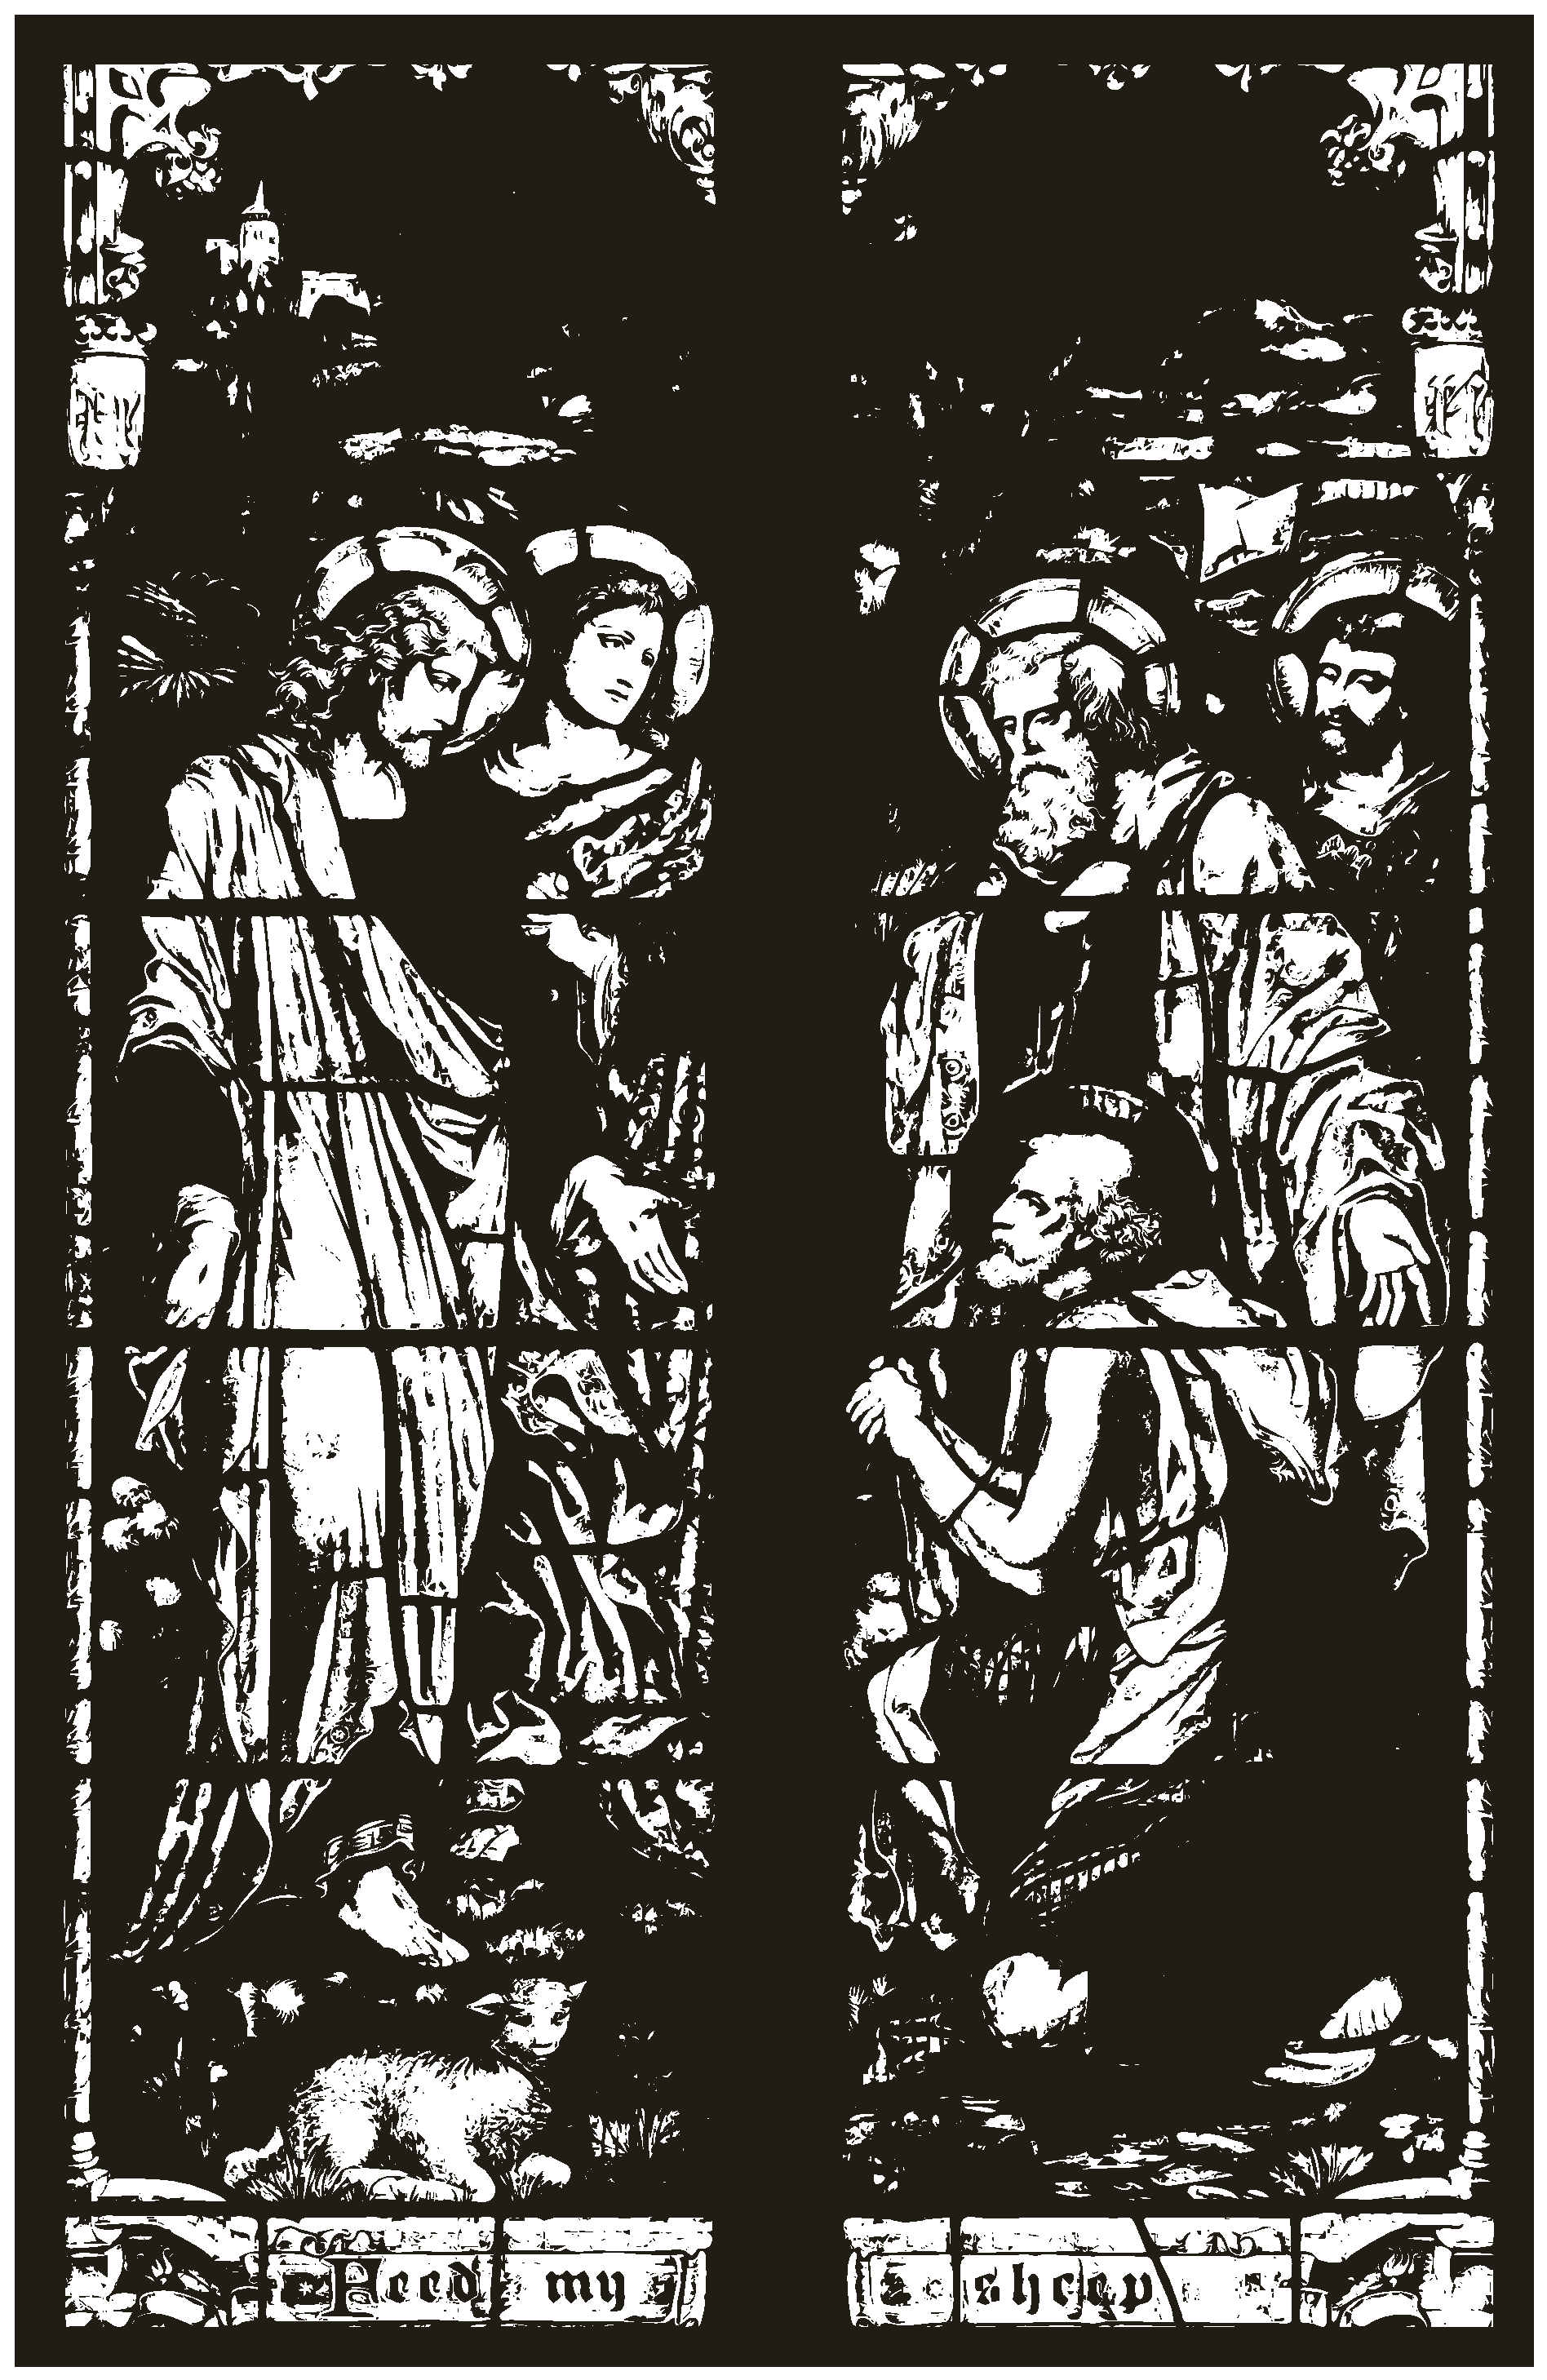
\includegraphics[scale=.25]{PFMS2.eps}
   \par
   \vspace{4ex}
   	\textsc{\Huge{The Pastoral Rites}}
   \end{center}
%\include{pages/Baptism.tex}
%\section{The Sacrament of Confirmation}
\fancyhead[RE,LO]{The Sacrament of Confirmation}

    Bishop. Our help is in the Name of the Lord;
    Answer. Who hath made heaven and earth.
    Bishop. Blessed be the Name of the Lord;
    Answer. Henceforth, world without end.
    Bishop. Lord, hear our prayer.
    Answer. And let our cry come unto thee.

Bishop. Let us pray.

ALMIGHTY and everliving God, who hast vouchsafed to regenerate these thy servants by Water and the Holy Ghost, and hast given unto them forgiveness of all their sins; Strengthen them, we beseech thee, O Lord, with the Holy Ghost, the Comforter, and daily increase in them thy manifold gifts of grace: the spirit of wisdom and under-standing, the spirit of counsel and ghostly strength, the spirit of knowledge and true godliness; and fill them, O Lord, with the spirit of thy holy fear, now and for ever. Amen. 
 

 
¶ Then all of them in order kneeling before the Bishop, he shall lay his hand upon the head of every one severally, saying,

DEFEND, O Lord, this thy Child with thy heavenly grace; that he may continue thine for ever; and daily increase in thy Holy Spirit more and more, until he come unto thy everlasting kingdom. Amen.

¶ Then shall the Bishop say,

Answer. 
The Lord be with you. 
And with thy spirit.
Bishop. Let us pray.

¶ Then shall the Bishop say the Lord's Prayer, the People kneeling and repeating it with him.

OUR Father, who art in heaven, Hallowed be thy Name. Thy kingdom come. Thy will be done, On earth as it is in heaven. Give us this day our daily bread. And forgive us our trespasses, As we forgive those who trespass against us. And lead us not into temptation, But deliver us from evil. For thine is the kingdom, and the power, and the glory, for ever and ever. Amen.

¶ Then shall the Bishop say,

ALMIGHTY and everliving God, who makest us both to will and to do those things which are good, and accept-able unto thy Divine Majesty; We make our humble supplications unto thee for these thy servants, upon whom, after the example of thy holy Apostles, we have now laid our hands, to certify them, by this sign, of thy favour and gracious goodness towards them. Let thy fatherly hand, we beseech thee, ever be over them; let thy Holy Spirit ever be with them; and so lead them in the knowledge and obedience of thy Word, that in the end they may obtain everlasting life; through our Lord Jesus Christ, who with thee and the same Holy Spirit liveth and reigneth ever, one God, world without end. Amen.

O ALMIGHTY Lord, and everlasting God, vouchsafe, we beseech thee, to direct, sanctify, and govern, both our hearts and bodies, in the ways of thy laws, and in the works of thy commandments; that, through thy most mighty protection, both here and ever, we may be pre served in body and soul; through our Lord and Saviour Jesus Christ. Amen.

¶ Then the Bishop shall bless them, saying thus,

THE Blessing of God Almighty, the Father, the Son, and the Holy Ghost, be upon you, and remain with you for ever. Amen.

¶ The Minister shall not omit earnestly to move the Persons confirmed to come, without delay, to the Lord’s Supper.

¶ And there shall none be admitted to the Holy Communion, until such time as he be confirmed, or be ready and desirous to be confirmed.
\section{The Sacrament of Penance}
\fancyhead[RE,LO]{The Sacrament of Penance}
\elcol{}{}
\textit{\scshape Penitent:} Bless me, Father, for I have sinned.\\
\textit{\scshape Priest:} The Lord be in thy heart and upon thy lips so that thou mayest meetly and rightly confess all thy sins: In the Name of the Father, {\ding{64}} and of the Son, and of the Holy Ghost. Amen.
\rub{The Penitent then confesses his sins using the following (or a similar) formula:}
I confess to God Almighty, to blessed Mary ever-Virgin, to blessed Michael the Archangel, to blessed John Baptist, to the holy Apostles Peter and Paul, to all the Saints, and to thee, father, that I have sinned exceedingly in thought, word, deed, and omission; by mine own great fault: since my last confession which was \inrub{indicate time since last confession}, when I received absolution and performed my penance, I have committed these sins: \inrub{indicate one's sins}. For these and all other sins which I cannot now remember, I am heartily sorry; I firmly purpose amendment; and ask pardon of God, and of thee, father, penance, counsel, and absolution.
\rub{Here the Priest gives penance, counsel, and then absolution saying:}

%\include{pages/Theological.tex}
%\section{The 32 Articles of the English Catholic Faith}
\fancyhead[RE,LO]{The 32 Articles}
\subsection{On Faith in the Most Holy Trinity}
\begin{enumerate}
	\item Of God the Father
	\begin{enumerate}[i.]
		\item There is one living and true God, the Father Almighty, everlasting, without body, parts, or passions; of infinite power, wisdom, and goodness; the Maker, and Preserver of all things both visible and invisible.
		\item The Father, himself unoriginate and uncaused, is the fountainhead (principium | ἀρχή) of the Trinity. The Father, being eternally Father, thus eternally, wholly, and perfectly begets his Son, who is the Word (Verbum | λόγος).
		\item Likewise, the Word is never without the Spirit. Therefore, God is Trinity: the Father simultaneously generating his Son and eternally, wholly, and perfectly spirating the Holy Ghost.
	\end{enumerate}
	\item Of God the Son
	\begin{enumerate}[i.]
		\item The Son, the Word of the Father, is begotten from everlasting of the Father, the very and eternal God, and of one substance with the Father.
		\item The Most Holy Trinity is the unique object of worship of the Catholic Church, because out of his infinite kindness and mercy, the Word made himself known to man by uniting human nature to his divine person. He is rightly said to be---as St. Justinian sets forth ---a single divine person who has a divine nature wholly from His Father to which is united, by composition and without division, an immaculate human nature wholly from Mary, his Mother.\fn{``For all the holy fathers in harmony teach us that nature or essence and form is one thing and hypostasis or person another, and that nature or essence and form indicate the universal, while hypostasis or person indicate the individual.''} Through the composite Christ, man is made able to truly partake of the divine nature.
		\item The Son, which is the Word of the Father, begotten from everlasting of the Father, the very and eternal God, and of one substance with the Father, took Man's nature in the womb of the blessed Virgin, of her substance: so that two whole and perfect Natures, that is to say, the Godhead and Manhood, were joined together in one Person, never to be divided, whereof is one Christ, very God, and very Man; who truly suffered, was crucified, dead, and buried, to reconcile his Father to us, and to be a sacrifice, not only for original guilt, but also for actual sins of men.
	\end{enumerate}
	\item Of God the Holy Ghost
	\begin{enumerate}[i.]
		\item The Holy Ghost, as St. John Damascene teaches, ``proceeds from the Father and rests in the Son.''\sn{On the Orthodox Faith I:8} As Sts. John Damascene and Photios teach, since the procession of the Holy Ghost is perfect, whole, and singular, the Father alone is the hypostatic origin (αἰτῐ́ᾱ) of the Holy Ghost.
		\item Likewise, as Sts. Augustine and John Damascene and Athanasius and Basil and Photios teach, the Son and Holy Ghost exist in eternal relationship with each other due to (a) their consubstantiality by their shared origin in the Father, (b) the mutual indwelling (circumincessio | περιχώρησις) of each person in the others, and (c) the unique rest the Holy Ghost has eternally in the Son.
		\item The Holy Ghost is the Gift of the Father for the Son. Therefore, he has the Father as his sole eternal efficient cause and the Son as his sole eternal final cause.
			\begin{enumerate}[a.]
				\item As St. Augustine teaches, it can be rightly said that the Holy Ghost proceeds (procedit) from both the Father and the Son. This understanding of procession indicates not origin but advancement of the Holy Ghost in the life of the Holy Trinity, so that---according to this Latin sense---the Holy Ghost proceeds from the Father as principle (principium, ᾰ̓ρχή),\sn{On the Trinity XV:26:47} from the Son as manifesting the communion between the Father and the Son, and from himself as the one who advances and exists in the eternal love of the Three Divine Persons.
				\item While the Latin sense of procession can be understood in an orthodox manner, as the West did of old, it is neither canonical nor wise for such theological speculation to be inserted into the Creed without the consent of an ecumenical council.
			\end{enumerate}
		\item Therefore, the Holy Ghost is of the same substance, majesty, glory, and operation (ἐνέργειᾰ) with the Father and the Son.
	\end{enumerate}
	\item Of the Unknowability of the Divine Nature
	\begin{enumerate}[i.]
		\item The nature of God is wholly and entirely incomprehensible. As St. Paul teaches, God ``alone has immortality, who dwells in unapproachable light, whom no one has ever seen or can see.''\sn{1 Tim. 6:16} Because of this---as St. John Damascene teaches---we can know the qualities surrounding the divine nature (τᾰ́ περῐ́ τήν φῠ́σῐν) but not the nature itself. Instead, it is only possible to know what the divine nature is not.
		\item Man comes to know God through seeing the co-equal and identical divine work of the three persons. As St. Gregory of Nyssa teaches, since the divine nature ``is exalted above the understanding of the questioners . . . it is absolutely necessary for us to be guided to the investigation of the Divine nature by its operations.''\sn{On the Holy Trinity 6}
		\item As the ecumenical councils---especially Chalcedon and Constantinople II---and St. Justinian teach, nature is not alone but hypostatised. Therefore, three hypostases subsist in the divine nature. Since the Father is not the Son and neither the Holy Ghost, an absolute lack of distinction between nature and person cannot be confessed but rather a true divine simplicity which confesses distinction between the persons themselves and between the persons and their unique common nature.
	\end{enumerate}
\end{enumerate}
\subsection{God's Revelation to Man}
\begin{enumerate}
\setcounter{enumi}{4}
	\item Of God's Knowability
	\begin{enumerate}[i.]
		\item Just as nature never exists alone but is hypostatised, likewise nature is never sterile and lifeless but energetic and operational. Therefore, in God, the incomprehensible divine nature is tri-hypostatised and eternally operating.
		\item This operation of God, just as the nature and hypostases, is truly divine and uncreated. By the Most Holy Trinity's divine operation, he gives himself freely to the regenerate out of divine clemency.
		\item Since the divine nature is incomprehensible, man is united to God through the Holy Ghost working in man so that man might become by grace what God is by nature.
		\item These operations of God---being divine and uncreated---neither divide the Holy Trinity into parts nor compromise the divine simplicity.
	\end{enumerate}
	\item Of the Purpose of the Incarnation
	\begin{enumerate}[i.]
		\item As St. Athanasius teaches, the Word becomes man for the salvation of mankind from sin and death. By the union of mankind and divinity in the person of Jesus Christ. The last Adam recapitulates in Himself wholly, perfectly, and charitably the failed life of the first Adam.
		\item At the Cross, Jesus Christ offers a full, perfect, and sufficient sacrifice as a propitiation to the Most Holy Trinity for the sins of the world. Full, perfect, and sufficient, because the infinite riches of God are offered, so that---unlike the sacrifices of the old covenant---there is nothing lacking in its efficacy, scope, or ability to achieve its purpose (the forgiveness of sins). Sacrifice, because the Victim is offered and suffers death by man unto God. Propitiation, because the sacrifice of the man is of infinite worth and provides for all that is lacking for the reconciliation between guilty man and the infinitely holy God. So that in this sweet exchange, as the Epistle to Diognetus terms it, ``the wickedness of many should be hid in a single righteous One, and that the righteousness of One should justify many transgressors!''
		\item Jesus Christ, receiving the Holy Ghost from his Father, likewise gives freely the Holy Ghost to his Body---the Church.
	\end{enumerate}
	\item Of the going down of Christ into Hell
	\begin{enumerate}[i.]
		\item As Christ died for us, and was buried, so also is it to be believed, that he went down into Hell to preach the Gospel to the souls there.
	\end{enumerate}
	\item Of the Resurrection of Christ
	\begin{enumerate}[i.]
		\item Christ did truly rise again from death, and took again his body, with flesh, bones, and all things appertaining to the perfection of Man's nature; wherewith he ascended into Heaven, and there sits, until he return to judge all Men at the last day.
		\item Human nature is so perfectly united to the Divine Word that all men, by the power of God, will be resurrected on the last day. As the Athanasian Creed confesses, ``At whose coming all men shall rise again with their bodies, and shall give account for their own works. And they that have done good shall go into life everlasting, and they that have done evil into everlasting fire.''
	\end{enumerate}
\item Of the Sufficiency of the Holy Scriptures
	\begin{enumerate}[i.]
		\item As St. Athanasius teaches, ``the sacred and inspired Scriptures are sufficient to declare the truth,''\sn{Against the Heathen 1:1} and contains all things necessary to salvation: so that whatsoever is not read therein, nor may be proved thereby, is not to be required of any man, that it should be believed as an article of the Faith, or be thought requisite or necessary to salvation.
		\item The traditions of the Church continue according to the guidance of the Spirit of Truth. Therefore, the authentic traditions of the Catholic Church cannot be rejected without impiety and error.
		\item As St. Augustine teaches, ``holy Scripture sets a rule to our teaching, that we dare not be wise more than it behooves to be wise . . . Be it not therefore for me to teach you any other thing, save to expound to you the words of the Teacher, and to treat of them as the Lord shall have given to me.''\sn{Of the Good of Widowhood 2}
		\item In the name of the Holy Scripture we do understand those canonical Books of the Old and New Testament, of whose authority was never any doubt in the Church. The Church rightly heeds the command of St. John Damascene to ``observe, further, that there are two and twenty books of the Old Testament, one for each letter of the Hebrew tongue,''\sn{On the Orthodox Faith IV:17}\fn{``For there are twenty-two letters of which five are double, and so they come to be twenty-seven. For the letters Caph, Mem, Nun, Pe , Sade are double. And thus the number of the books in this way is twenty-two, but is found to be twenty-seven because of the double character of five.''} as follows:
	\begin{multicols}{3}
	\begin{enumerate}[1.]
		\item Genesis
		\item Exodus
		\item Leviticus
		\item Numbers
		\item Deuteronomy
		\item Joshua
		\item Judges \& Ruth
		\item 1 \& 2 Samuel
		\item 1 \& 2 Kings
		\item 1 \& 2 Chronicles
		\item Job
		\item Psalms
		\item Proverbs
		\item Ecclesiastes
		\item Songs of Solomon
		\item The Twelve Prophets
		\item Isaiah
		\item Jeremiah
		\item Ezekiel
		\item Daniel
		\item 1 \& 2 Esdras
		\item Esther
	\end{enumerate}
	\end{multicols}
	\begin{multicols}{3}[All the Books of the New Testament, as they are commonly received, we do receive, and account them Canonical, being the following:]
	\begin{enumerate}[1.]
		\item Matthew
		\item Mark
		\item Luke
		\item John
		\item Acts of Apostles
		\item Romans
		\item 1 Corinthians
		\item 2 Corinthians
		\item Galatians
		\item Ephesians
		\item Philippians
		\item Colossians
		\item 1 Thessalonians
		\item 2 Thessalonians
		\item 1 Timothy
		\item 2 Timothy
		\item Titus
		\item Philemon
		\item Hebrews
		\item James
		\item 1 Peter
		\item 2 Peter
		\item 1 John
		\item 2 John
		\item 3 John
		\item Jude
		\item Revelation
	\end{enumerate}
	\end{multicols}
	\begin{multicols}{3}[And the other Books (as St. Jerome teaches) the Church reads for example of life and instruction of manners; but yet it does not apply them to establish any doctrine. These books, called ``Apocrypha'' by St. Jerome and ``Panaretus'' by St. John Damascene, ``are virtuous and noble, but are not counted nor were they placed in the ark,''\sn{On the Orthodox Faith IV:17} such are these following:]
		\begin{enumerate}[1.]
			\item 3 Esdras
			\item 4 Esdras
			\item Tobit
			\item Judith
			\item Psalm 151
			\item The rest of Esther
			\item Wisdom of Solomon
			\item Wisdom of Sirach
			\item Baruch the Prophet
			\item Epistle of Jeremiah
			\item Three Children's Song
			\item Story of Susanna
			\item Bel and the Dragon
			\item Prayer of Manasseh	
			\item 1 Maccabees
			\item 2 Maccabees
			\item 3 Maccabees
			\item 4 Maccabees
		\end{enumerate}
		\end{multicols}
		\item However, due to the catholic consent of the Church in her use of these books, they must be considered, even if not inspired, devoid of all impiety or error regarding faith and morals.
		\item The Sacred Scriptures, having God for its author---as a whole and in all of its parts---being perfectly authored by the same Holy Ghost who guides the Catholic Church, and being reposed within the same Church by the same Spirit, must always be interpreted according to the wisdom of the ecumenical councils and the unanimous consent of the Fathers, for the Catholic Church can never come to the knowledge of God except in a catholic mode.\fn{``It behooves those who preside over the churches, every day but especially on Lord's days, to teach all the clergy and people words of piety and of right religion, gathering out of holy Scripture meditations and determinations of the truth, and not going beyond the limits now fixed, nor varying from the tradition of the God-bearing fathers. And if any controversy in regard to Scripture shall have been raised, let them not interpret it otherwise than as the lights and doctors of the church in their writings have expounded it, and in those let them glory rather than in composing things out of their own heads, lest through their lack of skill they may have departed from what was fitting. For through the doctrine of the aforesaid fathers, the people coming to the knowledge of what is good and desirable, as well as what is useless and to be rejected, will remodel their life for the better, and not be led by ignorance, but applying their minds to the doctrine, they will take heed that no evil befall them and work out their salvation in fear of impending punishment.'' -Canon 19 of the Quinisext Council}
	\end{enumerate}
	\item Of the Old Testament.
	\begin{enumerate}[i.]
		\item The Old Testament is not contrary to the New: for both in the Old and New Testament everlasting life is offered to Mankind by Christ, who is the only Mediator between God and Man, being both God and Man. Wherefore they are not to be heard, which feign that the old Fathers did look only for transitory promises. Although the Law given from God by Moses, as touching Ceremonies and Rites, do not bind Christian men, nor the Civil precepts thereof ought of necessity to be received in any commonwealth; yet notwithstanding, no Christian man whatsoever is free from the obedience of the Commandments which are called Moral.
	\end{enumerate}
\end{enumerate}
\subsection{The Catholic Church}
\begin{enumerate}
\setcounter{enumi}{10}
	\item The Institution \& Mission of the Catholic Church
	\begin{enumerate}[i.]
		\item The Catholic Church is ``the Body of Christ,''\sn{1 Cor. 12:27; Eph. 4:12} because she is his bride, for whom he offers himself.\sn{Eph. 5:25; Rev. 19:7} Likewise, she is rightly called ``the People of God.''\sn{Judg. 20:2, Heb. 4:9} The Catholic Church---guided through the ages from the first Adam unto the last Adam, Jesus Christ, and unto the eschaton---is definitively and perfectly founded by Jesus Christ himself as the congregation of his new, final, and everlasting covenant.
		\item The Catholic Church is rightly called a perfect society (\textit{societas perfecta}). That is, she contains within herself all that is necessary for her purpose. Jesus Christ is the only head of the Catholic Church who governs, teaches, and cares for her.
			\begin{enumerate}[a.]
				\item Each particular church (a catholic bishop and his faithful) is fully a catholic church and the cell of the total society or communion.
			\end{enumerate}
		\item The Catholic Church---founded by Jesus Christ---is, as the West prays in its liturgy, ``firmly established upon the Rock of the Apostolic Confession''\sn{Collect for the Vigil of Sts. Peter \& Paul} by the Most Holy Trinity. Therefore, the apostolic faith is the efficient cause, constitutive element, and rule of the Catholic Church.
		\item The Holy Ghost is rightly called the soul, or animating principle, of the Body of Christ---the Church. The Holy Ghost is promised to be with the Catholic Church always, as the ``Spirit of truth'' who will ``guide you into all the truth.''\sn{Jn 16:12}
		\begin{enumerate}[a.]
			\item Since the Body of Christ is eternal, against which ``the gates of hell shall not prevail,''\sn{Mt 16:18} there can never be a time when the catholic faith is absent from, or abandoned by, the Catholic Church. Necessarily, then, any doctrine which is taught by the Catholic Church and believed, as St. Vincent of Lérins teaches, ``everywhere, always, by all,''\sn{Comm.2:6} cannot fail to be truly the catholic faith.
			\item Therefore, such teaching and reception by the Catholic Church, according to the divine promise in the Scriptures, is infallible.
		\end{enumerate}
		\item The entire work of the Catholic Church, including its liturgies and theology and almsgiving, is in fulfilment of its purpose: the salvation of souls. All its work and activity ultimately terminate in that end.
	\end{enumerate}
	\item Membership in the Catholic Church
	\begin{enumerate}[i.]
		\item The Catholic Church is ``the household of God, built on the foundation of the apostles and prophets, Christ Jesus himself being the cornerstone.''\sn{Eph. 2:19-20}
		\item The Church is rightly called a communion, that is, a joint partnership in the orthodox faith.
		\item A member is incorporated into the Church by Word \& Sacrament. As St. Basil teaches, ``first comes the confession, introducing us to salvation, and baptism follows, setting the seal upon our assent.''\sn{de Spiritu Sancto 12:28}
		\item A member cannot truly be incorporated into the Catholic Church without that catholic faith which is perfected in Baptism.
	\end{enumerate}
	\item The Ministry of the Catholic Church
	\begin{enumerate}[i.]
		\item Jesus Christ is rightly called the Apostle of the Father, for he is sent by the Father with his full authority. Likewise, he is rightly called the King of the Kingdom of God, for he is the natural heir of the kingdom according to his humanity and its rightful head according to his divinity. Furthermore, he is rightly called the ``the Shepherd and Bishop of your souls,''\sn{1 Pet 2:25} for he governs, teaches, and cares for his flock.
		\item Just as the Father sent Jesus Christ with his full authority, so Jesus Christ sent the apostles with his full authority for the governing, teaching, and caring for the particular churches throughout the world.\sn{Jn 20:20-1}
		\item The ministry of bishops (ἐπῐ́σκοποι), in true apostolic succession, continues the shepherding and governing of the churches of God.
		\begin{enumerate}[a.]
			\item As the earliest fathers---such as Sts. Clement and Ignatius---teach, the ministry of the new covenant is the fulfilment of the ministry of the old covenant.
			\item The full episcopal ministry is not contained merely in the Sacrament of Holy Orders. Rather, such sacrament, to be rightly administered, must be accompanied by jurisdiction over a particular church.
			\item The ministry of priests (πρεσβῠ́τεροι) is delegated by the bishops and serves to assist the bishops in their ministry, as delegated.
			\item The ministry of deacons (δῐᾱ́κονοι) is fundamentally a ministry of service at the direction of the bishop.
		\end{enumerate}
		\item According to the infinite wisdom of the Most Holy Trinity in his ordering of human sexuality and each sex's particular and unique and non-interchangeable role and purpose, only men---created by God and born as male---can be ordained into the major orders of bishop, priest, and deacon.
		\item For the good order of the Church, other minor orders, being non-sacramental, are---at different times---created and dissolved.
		\item While the Catholic Church is fully found in each true particular church, the canonical boundaries do not exhaust the Catholic Church.
	\end{enumerate}
	\item The Catholic Church rightly exercises her teaching authority through her bishops and the churches committed to their charge.
			\begin{enumerate}[a.]
				\item The bishops are canonically organised in a hierarchy among each other---in analogy of each particular church---seen most excellently in the Pentarchy of old, when elder Rome, having been orthodox, was truly the archbishop of archbishops.
			\end{enumerate}
		\item Since apostolic succession, in its totality, requires both the sacramental character and true jurisdiction; those who have received the Sacrament of Holy Orders but lack either the orthodox faith or jurisdiction do not have magisterial authority.
		\begin{enumerate}[a.]
			\item These commonly called \textit{episcopi vagantes} do not constitute true heads of particular churches and do not properly form true particular churches of the Catholic Church.
			\item Therefore, the universal teaching and reception of catholic \& orthodox doctrine (to which is ascribed infallibility) is not predicated of either these \textit{episcopi vagantes} or their congregations or any cleric who holds not the orthodox \& catholic faith joined with true \& ordinary jurisdiction.
		\end{enumerate}
	\item On Apostolic Succesion
		\begin{enumerate}[i.]
				\item Just as the old covenant had the high priest, the priests, and the Levites; likewise, in the new covenant is given a ministry of bishops, priests, and deacons.
				\item Jesus Christ is the true sufficient High Priest of the new covenant. He is the primordial high priest, bishop, and shepherd.
				\item Jesus Christ, as high priest, offered the full, perfect, and sufficient sacrifice of atonement in fulfilment of the old covenant shadow of the Feast of the Atonement.
				\item In the new covenant, there continues a need for sanctification (based on that sacrifice and its fruit) and the good order of the Church. Therefore, those sacerdotal and pastoral roles---with the appropriate authority---is held by Christ and delegated to others as his representatives (ᾰ̓πόστολοι).
				\item Therefore, the new covenant ministry can never be considered in addition to Jesus Christ or supplement to Jesus Christ but as the sufficient work of Jesus Christ through the instrument of his ministers.
		\end{enumerate}
	\item Of the Ecumenical Councils
	\begin{enumerate}[i.]
		\item The chief expression of the magisterial authority of the bishops is expressed in the ecumenical councils.
		\item When an ecumenical council teaches the orthodox faith and is received by the Catholic Church, it is rightly considered infallible and authentically ecumenical.
		\item The doctrines and canons of the ecumenical councils are binding upon the Catholic Church.
		\item There have been seven ancient and liturgically commemorated ecumenical councils.
		\begin{enumerate}[1.]
			\item Nicaea I
			\item Constantinople I
			\item Ephesus
			\item Chalcedon
			\item Constantinople II (including the Quinisext Council)
			\item Constantinople III
			\item Nicaea II
		\end{enumerate}
		\item Likewise, there have been others councils which have rightly taught the catholic faith and have been received by the Catholic Church:
		\begin{enumerate}[1.]
		\setcounter{enumiii}{7}
			\item Constantinople IV (879-880)
			\item Constantinople V (1351)
		\end{enumerate}
		\end{enumerate}
	\item Of the Creeds
	\begin{enumerate}[i.]
		\item The Three Creeds, Nicene Creed, Athanasius' Creed, and that which is commonly called the Apostles' Creed ought thoroughly to be received and believed: for they may be proved by most certain warrants of Holy Scripture and through the catholic consent of the Church.
	\end{enumerate}
	\end{enumerate}
\subsection{The Salvation of Man}
\begin{enumerate}
\setcounter{enumi}{18}
	\item Of Original Sin.
	\begin{enumerate}[i.]
		\item As all Mankind, during the state of Innocence, was in Adam; so in him all Men, falling from what he fell, remained in a State of Sin. Wherefore Mankind is become, not only subject unto Sin, but also, on Account of Sin, unto Punishment; which, according to the Sentence pronounced of GOD, was (Gen. 2:17), In the Day that thou eatest of the Tree, thou shalt surely die. And to this the Apostle alludes (Rom. 5:12), Wherefore as by one Man Sin entered into the World, and Death by Sin, and so Death passed upon all Men, for that all have sinned. So that we are conceived in our Mother’s Womb, and born in this Sin, according to the holy Psalmist (Psal. 51:7), Behold, I was shapen in Wickedness, and in Sin hath my Mother conceived me. This is called parental, or original Sin, first, because that, before this, Man was free from all Sin; although the Devil was then corrupt, and fallen, by whose Temptation this parental Sin sprang up in Man; and Adam becoming guilty, we all likewise, who descend from him, become also guilty. Secondly, this is called original Sin, because no Mortal is conceived without this Depravity of Nature.
		\item Original sin standeth not in the following of Adam, (as the Pelagians do vainly talk;) but it is the fault and corruption of the Nature of every man, that naturally is engendered of the offspring of Adam; whereby man is very far gone from original righteousness, and is of his own nature inclined to evil, so that the flesh lusteth always contrary to the Spirit; and therefore in every person born into this world, it deserveth God's wrath and damnation. And this infection of nature doth remain, yea in them that are regenerated; whereby the lust of the flesh, called in Greek, φρονημα σαρκος, (which some do expound the wisdom, some sensuality, some the affection, some the desire, of the flesh), is not subject to the Law of God. And although there is no condemnation for them that believe and are baptized; yet the Apostle doth confess, that concupiscence and lust hath of itself the nature of sin.
	\end{enumerate}
	\item Of Free-Will
	\begin{enumerate}[i.]
		\item The condition of Man after the fall of Adam is such, that he cannot turn and prepare himself, by his own natural strength and good works, to faith; and calling upon God. Wherefore we have no power to do good works pleasant and acceptable to God, without the grace of God by Christ preventing us, that we may have a good will, and working with us, when we have that good will.
	\end{enumerate}
	\item Of the Justification of Man
	\begin{enumerate}[i.]
		\item God, in his mercy, works in man to unite him through the Holy Ghost to Christ in reconciliation with the Father.
		\item This divinisation (θέωσις) begins at justification when man, having true confidence in the divine promises worked in him, is accounted righteous before God, only for the merit of our Lord and Saviour Jesus Christ by Faith, and not for his own works or deservings.
		\item When the Most Holy Trinity declares a man to be righteous, there is both a legal and a true change wrought in the man himself, since the Lord's words can never be without effect.
		\item As attested by the Sacred Scriptures and the Fathers, man is united to Jesus Christ and becomes by grace what he is by nature. However, sin and darkness co-exist with this divinisation as long as faith remains, for---as St. Basil teaches---``what saves us is our faith.''\sn{De Spiritu Sancto 18} And as St. Aelred teaches, ``let faith be for us, then, like the first day on which we believers are separated from unbelievers, as light from darkness,''\sn{Speculum Caritatis I:32:90} even though it is not until the seventh day---the eschaton---that ``all the darkness of error shall be dispersed.''\sn{Speculum Caritatis I:32:94}
		\item Faith (πῐ́στῐς) is not a mere intellectual assent to divinely revealed truths but a confidence and trust in the promises of God which is perfected and quickened by repentance. Mere intellectual assent is not worthy of the name ``faith.''
		\item As St. Basil teaches, divinising faith can exist in man before Baptism through the preaching of the Word, for ``faith is perfected through baptism, baptism is established through faith, and both are completed by the same names.''\sn{De Spiritu Sancto 12}
	\end{enumerate}
	\item Of Sanctification
	\begin{enumerate}[i.]
		\item After justification---or as the fulfilment of justification---the Holy Ghost further divinises the Christian through leading him into greater obedience to, and love of, God. Therefore, faith is necessarily fecund in producing good works, which are the fruits of Faith, and follow after Justification.
		\item Good works, not reconciling man with God as if lively faith was insufficient, heal the effects of sin in broken human nature. Since man is in Christ, and Christ lives in him, good works are pleasing and acceptable to God in Christ, and do spring out necessarily of a true and lively Faith insomuch that by them a lively Faith may be as evidently known as a tree discerned by the fruit.
		\item Therefore, where good works are not seen but, rather, wicked works and neglect of Christ's promises, the Catholic Church rightly judges a wicked man to be faithless and in need of penance.
	\end{enumerate}
	\item Of Glorification
	\begin{enumerate}[i.]
		\item Those elect, chosen ``in him before the foundation of the world,''\sn{Eph 1:4} who are justified and sanctified are, on the last day, reunited with their bodies and glorified.
		\item Such glorification is a full and complete divinisation of the human person.
		\item Before the eschaton, but after death, the full reward and judgement is not given to the faithful but a foretaste in Hades.
		\item Those who die in faith, united to Jesus Christ, do not fear death, for they trust in the promise that ``you will not abandon my soul to Sheol, or let your holy one see corruption.''\sn{Ps 16:10}
	\end{enumerate}
	\item Of Works before Justification
	\begin{enumerate}[i.]
		\item Works done before the grace of Christ, and the Inspiration of his Spirit, are not pleasant to God, forasmuch as they spring not of faith in Jesus Christ; neither do they make men meet to receive grace, or (as the School-authors say) deserve grace of congruity: yea rather, for that they are not done as God hath willed and commanded them to be done, we doubt not but they have the nature of sin.
	\end{enumerate}
	\item Of Christ without Sin
	\begin{enumerate}[i.]
		\item Christ in the truth of our nature was made like unto us in all things, sin only except, from which he was clearly void, both in his flesh, and in his spirit. He came to be the Lamb without spot, who, by sacrifice of himself once made, should take away the sins of the world; and sin (as Saint John says) was not in him. But all we the rest, although baptised and born again in Christ, yet offend in many things; and if we say we have no sin, we deceive ourselves, and the truth is not in us.
		\item Because Our Lord united an immaculate human nature to himself, it must be confessed that the sole source of his human nature, Mary the ever-Virgin Mother of God, also had an immaculate (Παναγία) human nature.
			\begin{enumerate}
				\item The heresy which supposes that the human nature, destined for the Word, could exist unhypostatised and be cleansed in such a supposed-state must be rejected, for by distorting the doctrine of the Mother of God, it distorts the doctrine of the Incarnate God himself.
				\item Likewise, the heresy which supposes that the human nature, united to Divine Word, was made immaculate by such union must also be rejected, for it would demote Christ the unique High Priest down to the level of every other high priest who ``offered for himself and for the people's sins committed in ignorance.''\sn{Heb 9:7}
			\end{enumerate}
	\end{enumerate}
	\item Of Predestination and Election
	\begin{enumerate}[i.]
		\item Predestination to Life is the everlasting purpose of God, whereby (before the foundations of the world were laid) he hath constantly decreed by his counsel secret to us, to deliver from curse and damnation those whom he hath chosen in Christ out of mankind, and to bring them by Christ to everlasting salvation, as vessels made to honour. Wherefore, they which be endued with so excellent a benefit of God, be called according to God's purpose by his Spirit working in due season: they through Grace obey the calling: they be justified freely: they be made sons of God by adoption: they be made like the image of his only-begotten Son Jesus Christ: they walk religiously in good works, and at length, by God's mercy, they attain to everlasting felicity.
		\item As the godly consideration of Predestination, and our Election in Christ, is full of sweet, pleasant, and unspeakable comfort to godly persons, and such as feel in themselves the working of the Spirit of Christ, mortifying the works of the flesh, and their earthly members, and drawing up their mind to high and heavenly things, as well because it doth greatly establish and confirm their faith of eternal Salvation to be enjoyed through Christ as because it doth fervently kindle their love towards God: So, for curious and carnal persons, lacking the Spirit of Christ, to have continually before their eyes the sentence of God's Predestination, is a most dangerous downfall, whereby the Devil doth thrust them either into desperation, or into wretchlessness of most unclean living, no less perilous than desperation.
		\item Furthermore, we must receive God's promises in such wise, as they be generally set forth to us in Holy Scripture: and, in our doings, that Will of God is to be followed, which we have expressly declared unto us in the Word of God.
	\end{enumerate}
	\end{enumerate}
\subsection{Of the Sacraments}
\begin{enumerate}
\setcounter{enumi}{26}
	\item In Our Lord's new covenant, he hath established seven sacraments for our salvation.
	\item Sacraments ordained of Christ be not only badges or tokens of Christian men's profession, but rather they be certain sure witnesses, and effectual signs of grace, and God's good will towards us, by the which he works invisibly in us, and does not only quicken, but also strengthen and confirm our Faith in him.
	\item The Sacraments were not ordained of Christ to be gazed upon, or to be carried about, but that we should duly use them.
	\item It is impious to celebrate or believe in the Sacraments in a manner contrary to the catholic and orthodox witness of the Fathers and the Church.
	\item There are two properly called Sacraments of the Gospel, for they are most illustriously promised by Jesus Christ in the Gospels and are generally necessary for salvation.
	\begin{enumerate}[i.]
		\item Baptism
			\begin{enumerate}[a.]
				\item Baptism is a mystery by which, when the body is washed in water, the soul of the believer is cleansed from sins by the Blood of Christ.
				\item This mystery was ordained by Christ himself, in the command which He gave his disciples.
				\item By means of this visible act he invisibly receives salvation of the soul, according to the promise of Christ.
			\end{enumerate}
		\item Eucharist
			\begin{enumerate}[a.]
				\item The Eucharist, or Communion, is a mystery in which the believer, under the form of bread, receives the Body itself of Christ; and under the form of wine, the Blood itself of Christ; for the remission of sins, and unto eternal life.
				\item Consequently, every true Christian ought to be persuaded that in this sublime mystery he does not receive simple bread and simple wine; but that, under the form of the hallowed bread, he receives the true Body itself of Christ, which was offered as a sacrifice upon the Cross for our salvation, and, like bread, was broken by many sufferings; and that, under the form of the hallowed wine, he receives the true Blood itself of Christ, which was poured forth from his pure side, and became the propitiation for all our sins. For when He gave the bread to his disciples the Lord said: ``This is my Body;'' and giving the wine He said, ``This is my Blood.''
				\item The Cup of the Lord is not to be denied to the Lay-people: for both the parts of the Lord's Sacrament, by Christ's ordinance and commandment, ought to be ministered to all Christian men alike.
			\end{enumerate}
	\end{enumerate}
	\item There are five others properly called Sacraments of the Church, for they are promised by Jesus Christ but revealed in the working of the early church in the Acts of the Apostles and are for the good order of the Catholic Church.
	\begin{enumerate}[i.]
	\setcounter{enumii}{2}
		\item Confirmation
			\begin{enumerate}[a.]
				\item Confirmation is a mystery by which, when the members of the body receive the imposition of hands and are anointed with chrism, there is poured forth upon the baptised person a spiritual unction; that is to say, the gifts of the Holy Ghost.
				\item This mystery is accomplished immediately after Baptism.
				\item By means of this sacred ordinance the Holy Ghost comes upon the baptised person, and seals---that is, confirms---him in the grace which he received at his Baptism; just as He came upon the disciples of Jesus Christ; and as the disciples themselves put their hands after Baptism on the believers, and by this laying on of the hands of the Apostles, those that were baptised received the Holy Ghost.
			\end{enumerate}
		\item Confession
			\begin{enumerate}[a.]
				\item Repentance is a mystery, through which the believer, knowing his sins, and having a firm trust in the mercies of Jesus Christ, receives the forgiveness of sins from God through the priest.
				%\item Not every deadly sin willingly committed after Baptism is sin against the Holy Ghost, and unpardonable. Wherefore the grant of repentance is not to be denied to such as fall into sin after Baptism. After we have received the Holy Ghost, we may depart from grace given, and fall into sin, and by the grace of God we may arise again, and amend our lives. And therefore they are to be condemned, which say, they can no more sin as long as they live here, or deny the place of forgiveness to such as truly repent.
			\end{enumerate}
		\item Unction of the Sick
			\begin{enumerate}[a.]
				\item Unction of the Sick is a mystery, in which the minister of the Church, anointing the sick person with oil, prays God to alleviate his malady and forgive his sins.
			\end{enumerate}
		\item Holy Orders
			\begin{enumerate}[a.]
				\item Priesthood is a mystery in which the Holy Ghost, by the hands of his ministers, ordains them that be rightly chosen to celebrate the mysteries and feed the flock of Christ.
				%\item In the Church, as a well-regulated society, there is a hierarchy; that is, an ecclesiastical government, constituted of the ecclesiastical presidents and rulers. The flock elect these spiritual rulers, and by this means the Lord Himself chooses the fit man.
				\item This ordination is effected by the invocation of the Holy Ghost, and the laying on of hands, at the time of assembly of the Church; which confirms the election.
				\item This ordination, effected by the imposition of hands, has its origin from the Apostles themselves, from whom it has been handed down from one to another, and come to us.
			\end{enumerate}
		\item Matrimony
			\begin{enumerate}[a.]
				\item Holy Matrimony is a mystery in which the minister of the Church crowns two persons to be united, and prays for the divine blessing upon them.
				\item The minister of the church joins them, and with all the Church beseeches God to grant them love, peace, and the blessing of children. And thus, by means of this ceremony, the bond becomes closer, as being confirmed before the altar of the Lord. This yoke can only be entered into between one man and one woman; for the Christian law does not by any means admit of polygamy.
				\item The intention and end of wedlock is the preservation of the human race. The man, as head of this relationship, should heartily love his wife, regarding her as his most faithful helpmate in the care and nourishment of his children; and not treat her harshly or cruelly, but correct her weakness with prudent forbearance. The duty of a woman is, to love and honour her own husband; that is, to accommodate her manners to his pleasure, and to submit even to ill-treatment with meekness of spirit. And they ought both to keep their marriage-bed blameless, and live together until death separates them.
				\item It is sinful, and truly impossible, to separate the purpose of procreation in the marital act from the purpose of mutual care and unity.
			\end{enumerate}
	\end{enumerate}
\end{enumerate}
%\include{pages/Devotions.tex}
 \fancyhead[RE,LO]{}
   \begin{center}
   	\textsc{
   	Most Holy Trinity, Save Us.\\
   	\small{
   	St. Mary Ever-Virgin, Pray for Us.\\
   	St. John the Divine, Pray for Us.\\
   	St. Alban the Martyr, Pray for Us.\\
   	St. Augustine of Canterbury, Pray for Us.\\
   	All Ye Holy Angels \& Saints, Pray for Us.
   	}
   	}
   	\vfill
   	\par
   	\includegraphics[scale=.2]{logo.eps}
			\par
	$\copyright$ 2025 Some Rights Reserved (CC-BY-SA-4.0)\\
	Apologia Anglicana, LLC\\
	\url{www.ApologiaAnglicana.org}
   \end{center}
\end{document}
